% !TEX root = ./Praxisbericht.tex
% https://github.com/James-Yu/LaTeX-Workshop/wiki/Compile
% ------------------------------------------------------------
% LaTeX Template für die DHBW zum Schnellstart!
% Original: https://github.wdf.sap.corp/vtgermany/LaTeX-Template-DHBW
% ------------------------------------------------------------
% ---- Präambel mit Angaben zum Dokument
% !TEX root = ../../Praxisbericht.tex
\documentclass[
    fontsize=12pt,           % Leitlinien sprechen von Schriftgröße 12.
    paper=A4,
    twoside=false,
    listof=totoc,            % Tabellen- und Abbildungsverzeichnis ins Inhaltsverzeichnis
    bibliography=totoc,      % Literaturverzeichnis ins Inhaltsverzeichnis aufnehmen
    titlepage,               % Titlepage-Umgebung anstatt \maketitle
    headsepline,             % horizontale Linie unter Kolumnentitel
    abstract,                % Überschrift einschalten, Abstract muss in {abstract}-Umgebung stehen
    % final,                 % TODO:FINAL_COMPILATION Remove or change to final [final or draft]
]{scrreprt}                  % Verwendung von KOMA-Report
\pdfcompresslevel=0          % TODO:FINAL_COMPILATION Remove
\pdfobjcompresslevel=0       % TODO:FINAL_COMPILATION Remove

\usepackage[T1]{fontenc}     % Ausgabe von westeuropäischen Zeichen (auch Umlaute)
\usepackage{alphabeta}       % Griechische Buchstaben
\usepackage[utf8]{inputenc}  % UTF8 Encoding einschalten
\usepackage[ngerman]{babel}  % Neue deutsche Rechtschreibung
\usepackage{microtype}       % Trennung von Wörtern wird besser umgesetzt
\usepackage{lmodern}         % Nicht-gerasterte Schriftarten (bei MikTeX erforderlich)
\usepackage[draft]{graphicx} % Einbinden von Grafiken erlauben % TODO:FINAL_COMPILATION Remove or change to final [final or draft] single one can be viewed with \includegraphics[draft=false]{image.pdf}
\usepackage{wrapfig}         % Grafiken fließend im Text
\usepackage{setspace}        % Zeilenabstand \singlespacing, \onehalfspaceing, \doublespacing
\usepackage[
    %showframe,                % Ränder anzeigen lassen
    left=2.7cm, right=2.5cm,
    top=2.5cm,  bottom=2.5cm,
    includeheadfoot,
    showframe=false,             % TODO:FINAL_COMPILATION Remove
]{geometry}                      % Seitenlayout einstellen
\usepackage{scrlayer-scrpage}    % Gestaltung von Fuß- und Kopfzeilen
\KOMAoptions{draft=false}        % TODO:FINAL_COMPILATION Change to false
\usepackage{acronym}             % Abkürzungen, Abkürzungsverzeichnis
\usepackage{titletoc}            % Anpassungen am Inhaltsverzeichnis
\contentsmargin{0.75cm}          % Abstand im Inhaltsverzeichnis zw. Punkt und Seitenzahl
\usepackage[                     % Klickbare Links (enth. auch "nameref", "url" Package)
    hidelinks,                     % Blende die "URL Boxen" aus.
    breaklinks=true                % Breche zu lange URLs am Zeilenende um
]{hyperref}
\usepackage[hypcap=true, justification=centering]{caption}% Anker Anpassung für Referenzen
\urlstyle{same}                  % Aktuelle Schrift auch für URLs
% Anpassung von autoref für Gleichungen (ergänzt runde Klammern) und Algorithm.
% Anstatt "Listing" kann auch z.B. "Code-Ausschnitt" verwendet werden. Dies sollte
% jedoch synchron gehalten werden mit \lstlistingname (siehe weiter unten).
\addto\extrasngerman{%
    \def\equationautorefname~#1\null{Gleichung~(#1)\null}
    \def\lstnumberautorefname{Zeile}
    \def\lstlistingautorefname{Listing}
    \def\algorithmautorefname{Algorithmus}
    % Damit einheitlich "Abschnitt 1.2[.3]" verwendet wird und nicht "Unterabschnitt 1.2.3"
    % \def\subsectionautorefname{Abschnitt}
}

% ---- Abstand verkleinern von der Überschrift
\renewcommand*{\chapterheadstartvskip}{\vspace*{.5\baselineskip}}

% Hierdurch werden Schusterjungen und Hurenkinder vermieden, d.h. einzelne Wörter
% auf der nächsten Seite oder in einer einzigen Zeile.
% LaTeX kann diese dennoch erzeugen, falls das Layout ansonsten nicht umsetzbar ist.
% Diese Werte sind aber gute Startwerte.
\widowpenalty10000
\clubpenalty10000

% ---- Für das Quellenverzeichnis
\usepackage[
    backend = biber,                % Verweis auf biber
    language = auto,
    style = numeric,                % Nummerierung der Quellen mit Zahlen
    sorting = none,                 % none = Sortierung nach der Erscheinung im Dokument
    sortcites = true,               % Sortiert die Quellen innerhalb eines cite-Befehls
    block = space,                  % Extra Leerzeichen zwischen Blocks
    hyperref = true,                % Links sind klickbar auch in der Quelle
    %backref = true,                % Referenz, auf den Text an die zitierte Stelle
    bibencoding = auto,
    giveninits = true,              % Vornamen werden abgekürzt
    doi=false,                      % DOI nicht anzeigen
    isbn=false,                     % ISBN nicht anzeigen
    alldates=short                  % Datum immer als DD.MM.YYYY anzeigen
]{biblatex}
\addbibresource{Inhalt/literatur.bib}
\setcounter{biburlnumpenalty}{3000}     % Umbruchgrenze für Zahlen
\setcounter{biburlucpenalty}{6000}      % Umbruchgrenze für Großbuchstaben
\setcounter{biburllcpenalty}{9000}      % Umbruchgrenze für Kleinbuchstaben
\DeclareNameAlias{default}{family-given}  % Nachname vor dem Vornamen
\AtBeginBibliography{\renewcommand{\multinamedelim}{\addslash\space
    }\renewcommand{\finalnamedelim}{\multinamedelim}}  % Schrägstrich zwischen den Autorennamen
\DefineBibliographyStrings{german}{
    urlseen = {Einsichtnahme:},                      % Ändern des Titels von "besucht am"
}
\usepackage[babel,german=quotes]{csquotes}         % Deutsche Anführungszeichen + Zitate


% ---- Für Mathevorlage
\usepackage{amsmath}    % Erweiterung vom Mathe-Satz
\usepackage{amssymb}    % Lädt amsfonts und weitere Symbole
\usepackage{amsfonts}
\usepackage{MnSymbol}   % Für Symbole, die in amssymb nicht enthalten sind.
\usepackage{mathtools}
\usepackage{scrextend}
\setcounter{MaxMatrixCols}{40}

% ---- Für Quellcodevorlage
\usepackage{scrhack}                    % Hack zur Verw. von listings in KOMA-Script
\usepackage{listings}                   % Darstellung von Quellcode
\usepackage[table,xcdraw]{xcolor}       % Einfache Verwendung von Farben
% -- Eigene Farben für den Quellcode
\definecolor{JavaLila}{rgb}{0.4,0.1,0.4}
\definecolor{JavaGruen}{rgb}{0.3,0.5,0.4}
\definecolor{JavaBlau}{rgb}{0.0,0.0,1.0}
\definecolor{ABAPKeywordsBlue}{HTML}{6000ff}
\definecolor{ABAPCommentGrey}{HTML}{808080}
\definecolor{ABAPStringGreen}{HTML}{4da619}
\definecolor{PyKeywordsBlue}{HTML}{0000AC}
\definecolor{PyCommentGrey}{HTML}{808080}
\definecolor{PyStringGreen}{HTML}{008080}
% -- Farben für ABAP CDS
\definecolor{CDSString}{HTML}{FF8C00}
\definecolor{CDSKeywords}{HTML}{6000ff}
\definecolor{CDSAnnotation}{HTML}{00BFFF}
\definecolor{CDSComment}{HTML}{808080}
\definecolor{CDSFunc}{HTML}{FF0000}

% -- Default Listing-Styles

\lstset{
% Das Paket "listings" kann kein UTF-8. Deswegen werden hier
% die häufigsten Zeichen definiert (ä,ö,ü,...)
literate=%
    {á}{{\'a}}1 {é}{{\'e}}1 {í}{{\'i}}1 {ó}{{\'o}}1 {ú}{{\'u}}1
{Á}{{\'A}}1 {É}{{\'E}}1 {Í}{{\'I}}1 {Ó}{{\'O}}1 {Ú}{{\'U}}1
{à}{{\`a}}1 {è}{{\`e}}1 {ì}{{\`i}}1 {ò}{{\`o}}1 {ù}{{\`u}}1
{À}{{\`A}}1 {È}{{\'E}}1 {Ì}{{\`I}}1 {Ò}{{\`O}}1 {Ù}{{\`U}}1
{ä}{{\"a}}1 {ë}{{\"e}}1 {ï}{{\"i}}1 {ö}{{\"o}}1 {ü}{{\"u}}1
{Ä}{{\"A}}1 {Ë}{{\"E}}1 {Ï}{{\"I}}1 {Ö}{{\"O}}1 {Ü}{{\"U}}1
{â}{{\^a}}1 {ê}{{\^e}}1 {î}{{\^i}}1 {ô}{{\^o}}1 {û}{{\^u}}1
{Â}{{\^A}}1 {Ê}{{\^E}}1 {Î}{{\^I}}1 {Ô}{{\^O}}1 {Û}{{\^U}}1
{œ}{{\oe}}1 {Œ}{{\OE}}1 {æ}{{\ae}}1 {Æ}{{\AE}}1 {ß}{{\ss}}1
{ű}{{\H{u}}}1 {Ű}{{\H{U}}}1 {ő}{{\H{o}}}1 {Ő}{{\H{O}}}1
{ç}{{\c c}}1 {Ç}{{\c C}}1 {ø}{{\o}}1 {å}{{\r a}}1 {Å}{{\r A}}1
{€}{{\euro}}1 {£}{{\pounds}}1 {«}{{\guillemotleft}}1
{»}{{\guillemotright}}1 {ñ}{{\~n}}1 {Ñ}{{\~N}}1 {¿}{{?`}}1,
breaklines=true,        % Breche lange Zeilen um
breakatwhitespace=true, % Wenn möglich, bei Leerzeichen umbrechen
% Symbol für Zeilenumbruch einfügen
prebreak=\raisebox{0ex}[0ex][0ex]{\ensuremath{\rhookswarrow}},
postbreak=\raisebox{0ex}[0ex][0ex]{\ensuremath{\rcurvearrowse\space}},
tabsize=4,                                 % Setze die Breite eines Tabs
basicstyle=\ttfamily\small,                % Grundsätzlicher Schriftstyle
columns=fixed,                             % Besseres Schriftbild
numbers=left,                              % Nummerierung der Zeilen
%frame=single,                             % Umrandung des Codes
showstringspaces=false,                    % Keine Leerzeichen hervorheben
keywordstyle=\color{blue},
ndkeywordstyle=\bfseries\color{darkgray},
identifierstyle=\color{black},
commentstyle=\itshape\color{JavaGruen},   % Kommentare in eigener Farbe
stringstyle=\color{JavaBlau},             % Strings in eigener Farbe,
captionpos=b,                             % Bild*unter*schrift
xleftmargin=5.0ex
}

% ---- Eigener JAVA-Style für den Quellcode
\renewcommand{\ttdefault}{pcr}               % Schriftart, welche auch fett beinhaltet
\lstdefinestyle{EigenerJavaStyle}{
    language=Java,                             % Syntax Highlighting für Java
    %frame=single,                             % Umrandung des Codes
    keywordstyle=\bfseries\color{JavaLila},    % Keywords in eigener Farbe und fett
    commentstyle=\itshape\color{JavaGruen},    % Kommentare in eigener Farbe und italic
    stringstyle=\color{JavaBlau}               % Strings in eigener Farbe
}

% ---- Eigener ABAP-Style für den Quellcode
\renewcommand{\ttdefault}{pcr}
\lstdefinestyle{EigenerABAPStyle}{
    language=[R/3 6.10]ABAP,
    morestring=[b]\|,                          % Für Pipe-Strings
    morestring=[b]\`,                          % für Backtick-Strings
    keywordstyle=\bfseries\color{ABAPKeywordsBlue},
    commentstyle=\itshape\color{ABAPCommentGrey},
    stringstyle=\color{ABAPStringGreen},
    tabsize=2,
    morekeywords={
            types,
            @data,
            as,
            lower,
            start,
            selection,
            order,
            by,
            inner,
            join,
            key,
            end,
            cast,
            optional,
            returning,
            badi,
            default,
            standard,
            length,
            begin,
            filters,
            final,
            global,
            friends,
            interfaces,
            endclass,
            endinterface,
            interface,
            implementation,
            eq,
            lt,
            gt,
            index,
            reference,
            symbol,
            assigning
        }
}

% ---- Eigener Python-Style für den Quellcode
\renewcommand{\ttdefault}{pcr}
\lstdefinestyle{EigenerPythonStyle}{
    language=Python,
    columns=flexible,
    keywordstyle=\bfseries\color{PyKeywordsBlue},
    commentstyle=\itshape\color{PyCommentGrey},
    stringstyle=\color{PyStringGreen}
}

%----- ABAP-CDS-View language
\lstdefinelanguage{ABAPCDS}{
    sensitive=false,
    %Keywords
    morekeywords={define,
            view,
            as,
            select,
            from,
            inner,
            join,
            on,
            key,
            case,
            when,
            then,
            else,
            end,
            true,
            false,
            cast,
            where,
            and,
            distinct,
            group,
            by,
            having,
            min,
            sum,
            max,
            count,
            avg
        },
    %Methoden
    morekeywords=[2]{
            div,
            currency\_conversion,
            dats\_days\_between,
            concat\_with\_space,
            dats\_add_days,
            dats\_is\_valid,
            dats\_add\_months,
            unit\_conversion,
            division,
            mod,
            abs,
            floor,
            ceil,
            round,
            concat,
            replace,
            substring,
            left,
            right,
            length
        },
    morecomment=[s][\color{CDSAnnotation}]{@}{:},
    morecomment=[l][\itshape\color{CDSComment}]{//},
    morecomment=[s][\itshape\color{CDSComment}]{/*}{*/},
    morestring=[b][\color{CDSString}]',
    keywordstyle=\bfseries\color{CDSKeywords},
    keywordstyle=[2]\color{CDSFunc}
}

% ---- JavaScript
\lstdefinelanguage{JavaScript}{
    morekeywords=[1]{await, async, break, case, catch, class, const, constructor, continue, debugger, default, delete, do, else, enum, export, extends, finally, for, from, function, if, implements, import, in, instanceof, new, return, super, switch, this, throw, try, typeof, var, void, while, with, yield, get, set, static, of, let, throw, try},
    % Literals, primitive types, and reference types.
    morekeywords=[2]{false, null, true, boolean, number, undefined,
            Array, Boolean, Date, Math, Number, String, Object, NaN, Symbol},
    % Built-ins.
    morekeywords=[3]{eval, parseInt, parseFloat, escape, unescape},
    sensitive=true,
    morecomment=[s]{/*}{*/},
    morecomment=[l]//,
    morecomment=[s]{/**}{*/}, % JavaDoc style comments
    morestring=[b]',
    morestring=[b]",
    morestring=[b]` % Interpolation strings.
}

% ---- TypeScript
\renewcommand{\ttdefault}{pcr}
\lstdefinestyle{Typescript}{
    language=JavaScript,
    morekeywords={
            type,
            interface,
            as,
            implements,
            package,
            namespace,
            private,
            protected,
            public,
            any,
            unknown,
            declare,
            module,
            require,
            from,
            symbol,
            keyof,
            infer,
            abstract
        }
}


\lstdefinelanguage{Rust}{%
  sensitive%
, morecomment=[l]{//}%
, morecomment=[s]{/*}{*/}%
, moredelim=[s][{\itshape\color[rgb]{0,0,0.75}}]{\#[}{]}%
, morestring=[b]{"}%
, alsodigit={}%
, alsoother={}%
, alsoletter={!}%
%
%
% [1] reserve keywords
% [2] traits
% [3] primitive types
% [4] type and value constructors
% [5] identifier
%
, morekeywords={break, continue, else, for, if, in, loop, match, return, while}  % control flow keywords
, morekeywords={as, const, let, move, mut, ref, static}  % in the context of variables
, morekeywords={dyn, enum, fn, impl, Self, self, struct, trait, type, union, use, where}  % in the context of declarations
, morekeywords={crate, extern, mod, pub, super}  % in the context of modularisation
, morekeywords={unsafe}  % markers
, morekeywords={abstract, alignof, become, box, do, final, macro, offsetof, override, priv, proc, pure, sizeof, typeof, unsized, virtual, yield}  % reserved identifiers
%
% grep 'pub trait [A-Za-z][A-Za-z0-9]*' -r . | sed 's/^.*pub trait \([A-Za-z][A-Za-z0-9]*\).*/\1/g' | sort -u | tr '\n' ',' | sed 's/^\(.*\),$/{\1}\n/g' | sed 's/,/, /g'
, morekeywords=[2]{Add, AddAssign, Any, AsciiExt, AsInner, AsInnerMut, AsMut, AsRawFd, AsRawHandle, AsRawSocket, AsRef, Binary, BitAnd, BitAndAssign, Bitor, BitOr, BitOrAssign, BitXor, BitXorAssign, Borrow, BorrowMut, Boxed, BoxPlace, BufRead, BuildHasher, CastInto, CharExt, Clone, CoerceUnsized, CommandExt, Copy, Debug, DecodableFloat, Default, Deref, DerefMut, DirBuilderExt, DirEntryExt, Display, Div, DivAssign, DoubleEndedIterator, DoubleEndedSearcher, Drop, EnvKey, Eq, Error, ExactSizeIterator, ExitStatusExt, Extend, FileExt, FileTypeExt, Float, Fn, FnBox, FnMut, FnOnce, Freeze, From, FromInner, FromIterator, FromRawFd, FromRawHandle, FromRawSocket, FromStr, FullOps, FusedIterator, Generator, Hash, Hasher, Index, IndexMut, InPlace, Int, Into, IntoCow, IntoInner, IntoIterator, IntoRawFd, IntoRawHandle, IntoRawSocket, IsMinusOne, IsZero, Iterator, JoinHandleExt, LargeInt, LowerExp, LowerHex, MetadataExt, Mul, MulAssign, Neg, Not, Octal, OpenOptionsExt, Ord, OsStrExt, OsStringExt, Packet, PartialEq, PartialOrd, Pattern, PermissionsExt, Place, Placer, Pointer, Product, Put, RangeArgument, RawFloat, Read, Rem, RemAssign, Seek, Shl, ShlAssign, Shr, ShrAssign, Sized, SliceConcatExt, SliceExt, SliceIndex, Stats, Step, StrExt, Sub, SubAssign, Sum, Sync, TDynBenchFn, Terminal, Termination, ToOwned, ToSocketAddrs, ToString, Try, TryFrom, TryInto, UnicodeStr, Unsize, UpperExp, UpperHex, WideInt, Write}
, morekeywords=[2]{Send}  % additional traits
%
, morekeywords=[3]{bool, char, f32, f64, i8, i16, i32, i64, isize, str, u8, u16, u32, u64, unit, usize, i128, u128}  % primitive types
%
, morekeywords=[4]{Err, false, None, Ok, Some, true}  % prelude value constructors
% grep 'pub \(type\|struct\|enum\) [A-Za-z][A-Za-z0-9]*' -r . | sed 's/^.*pub \(type\|struct\|enum\) \([A-Za-z][A-Za-z0-9]*\).*/\2/g' | sort -u | tr '\n' ',' | sed 's/^\(.*\),$/{\1}\n/g' | sed 's/,/, /g'
, morekeywords=[3]{AccessError, Adddf3, AddI128, AddoI128, AddoU128, ADDRESS, ADDRESS64, addrinfo, ADDRINFOA, AddrParseError, Addsf3, AddU128, advice, aiocb, Alignment, AllocErr, AnonPipe, Answer, Arc, Args, ArgsInnerDebug, ArgsOs, Argument, Arguments, ArgumentV1, Ashldi3, Ashlti3, Ashrdi3, Ashrti3, AssertParamIsClone, AssertParamIsCopy, AssertParamIsEq, AssertUnwindSafe, AtomicBool, AtomicPtr, Attr, auxtype, auxv, BackPlace, BacktraceContext, Barrier, BarrierWaitResult, Bencher, BenchMode, BenchSamples, BinaryHeap, BinaryHeapPlace, blkcnt, blkcnt64, blksize, BOOL, boolean, BOOLEAN, BoolTrie, BorrowError, BorrowMutError, Bound, Box, bpf, BTreeMap, BTreeSet, Bucket, BucketState, Buf, BufReader, BufWriter, Builder, BuildHasherDefault, BY, BYTE, Bytes, CannotReallocInPlace, cc, Cell, Chain, CHAR, CharIndices, CharPredicateSearcher, Chars, CharSearcher, CharsError, CharSliceSearcher, CharTryFromError, Child, ChildPipes, ChildStderr, ChildStdin, ChildStdio, ChildStdout, Chunks, ChunksMut, ciovec, clock, clockid, Cloned, cmsgcred, cmsghdr, CodePoint, Color, ColorConfig, Command, CommandEnv, Component, Components, CONDITION, condvar, Condvar, CONSOLE, CONTEXT, Count, Cow, cpu, CRITICAL, CStr, CString, CStringArray, Cursor, Cycle, CycleIter, daddr, DebugList, DebugMap, DebugSet, DebugStruct, DebugTuple, Decimal, Decoded, DecodeUtf16, DecodeUtf16Error, DecodeUtf8, DefaultEnvKey, DefaultHasher, dev, device, Difference, Digit32, DIR, DirBuilder, dircookie, dirent, dirent64, DirEntry, Discriminant, DISPATCHER, Display, Divdf3, Divdi3, Divmoddi4, Divmodsi4, Divsf3, Divsi3, Divti3, dl, Dl, Dlmalloc, Dns, DnsAnswer, DnsQuery, dqblk, Drain, DrainFilter, Dtor, Duration, DwarfReader, DWORD, DWORDLONG, DynamicLibrary, Edge, EHAction, EHContext, Elf32, Elf64, Empty, EmptyBucket, EncodeUtf16, EncodeWide, Entry, EntryPlace, Enumerate, Env, epoll, errno, Error, ErrorKind, EscapeDebug, EscapeDefault, EscapeUnicode, event, Event, eventrwflags, eventtype, ExactChunks, ExactChunksMut, EXCEPTION, Excess, ExchangeHeapSingleton, exit, exitcode, ExitStatus, Failure, fd, fdflags, fdsflags, fdstat, ff, fflags, File, FILE, FileAttr, filedelta, FileDesc, FilePermissions, filesize, filestat, FILETIME, filetype, FileType, Filter, FilterMap, Fixdfdi, Fixdfsi, Fixdfti, Fixsfdi, Fixsfsi, Fixsfti, Fixunsdfdi, Fixunsdfsi, Fixunsdfti, Fixunssfdi, Fixunssfsi, Fixunssfti, Flag, FlatMap, Floatdidf, FLOATING, Floatsidf, Floatsisf, Floattidf, Floattisf, Floatundidf, Floatunsidf, Floatunsisf, Floatuntidf, Floatuntisf, flock, ForceResult, FormatSpec, Formatted, Formatter, Fp, FpCategory, fpos, fpos64, fpreg, fpregset, FPUControlWord, Frame, FromBytesWithNulError, FromUtf16Error, FromUtf8Error, FrontPlace, fsblkcnt, fsfilcnt, fsflags, fsid, fstore, fsword, FullBucket, FullBucketMut, FullDecoded, Fuse, GapThenFull, GeneratorState, gid, glob, glob64, GlobalDlmalloc, greg, group, GROUP, Guard, GUID, Handle, HANDLE, Handler, HashMap, HashSet, Heap, HINSTANCE, HMODULE, hostent, HRESULT, id, idtype, if, ifaddrs, IMAGEHLP, Immut, in, in6, Incoming, Infallible, Initializer, ino, ino64, inode, input, InsertResult, Inspect, Instant, int16, int32, int64, int8, integer, IntermediateBox, Internal, Intersection, intmax, IntoInnerError, IntoIter, IntoStringError, intptr, InvalidSequence, iovec, ip, IpAddr, ipc, Ipv4Addr, ipv6, Ipv6Addr, Ipv6MulticastScope, Iter, IterMut, itimerspec, itimerval, jail, JoinHandle, JoinPathsError, KDHELP64, kevent, kevent64, key, Key, Keys, KV, l4, LARGE, lastlog, launchpad, Layout, Lazy, lconv, Leaf, LeafOrInternal, Lines, LinesAny, LineWriter, linger, linkcount, LinkedList, load, locale, LocalKey, LocalKeyState, Location, lock, LockResult, loff, LONG, lookup, lookupflags, LookupHost, LPBOOL, LPBY, LPBYTE, LPCSTR, LPCVOID, LPCWSTR, LPDWORD, LPFILETIME, LPHANDLE, LPOVERLAPPED, LPPROCESS, LPPROGRESS, LPSECURITY, LPSTARTUPINFO, LPSTR, LPVOID, LPWCH, LPWIN32, LPWSADATA, LPWSAPROTOCOL, LPWSTR, Lshrdi3, Lshrti3, lwpid, M128A, mach, major, Map, mcontext, Metadata, Metric, MetricMap, mflags, minor, mmsghdr, Moddi3, mode, Modsi3, Modti3, MonitorMsg, MOUNT, mprot, mq, mqd, msflags, msghdr, msginfo, msglen, msgqnum, msqid, Muldf3, Mulodi4, Mulosi4, Muloti4, Mulsf3, Multi3, Mut, Mutex, MutexGuard, MyCollection, n16, NamePadding, NativeLibBoilerplate, nfds, nl, nlink, NodeRef, NoneError, NonNull, NonZero, nthreads, NulError, OccupiedEntry, off, off64, oflags, Once, OnceState, OpenOptions, Option, Options, OptRes, Ordering, OsStr, OsString, Output, OVERLAPPED, Owned, Packet, PanicInfo, Param, ParseBoolError, ParseCharError, ParseError, ParseFloatError, ParseIntError, ParseResult, Part, passwd, Path, PathBuf, PCONDITION, PCONSOLE, Peekable, PeekMut, Permissions, PhantomData, pid, Pipes, PlaceBack, PlaceFront, PLARGE, PoisonError, pollfd, PopResult, port, Position, Powidf2, Powisf2, Prefix, PrefixComponent, PrintFormat, proc, Process, PROCESS, processentry, protoent, PSRWLOCK, pthread, ptr, ptrdiff, PVECTORED, Queue, radvisory, RandomState, Range, RangeFrom, RangeFull, RangeInclusive, RangeMut, RangeTo, RangeToInclusive, RawBucket, RawFd, RawHandle, RawPthread, RawSocket, RawTable, RawVec, Rc, ReadDir, Receiver, recv, RecvError, RecvTimeoutError, ReentrantMutex, ReentrantMutexGuard, Ref, RefCell, RefMut, REPARSE, Repeat, Result, Rev, Reverse, riflags, rights, rlim, rlim64, rlimit, rlimit64, roflags, Root, RSplit, RSplitMut, RSplitN, RSplitNMut, RUNTIME, rusage, RwLock, RWLock, RwLockReadGuard, RwLockWriteGuard, sa, SafeHash, Scan, sched, scope, sdflags, SearchResult, SearchStep, SECURITY, SeekFrom, segment, Select, SelectionResult, sem, sembuf, send, Sender, SendError, servent, sf, Shared, shmatt, shmid, ShortReader, ShouldPanic, Shutdown, siflags, sigaction, SigAction, sigevent, sighandler, siginfo, Sign, signal, signalfd, SignalToken, sigset, sigval, Sink, SipHasher, SipHasher13, SipHasher24, size, SIZE, Skip, SkipWhile, Slice, SmallBoolTrie, sockaddr, SOCKADDR, sockcred, Socket, SOCKET, SocketAddr, SocketAddrV4, SocketAddrV6, socklen, speed, Splice, Split, SplitMut, SplitN, SplitNMut, SplitPaths, SplitWhitespace, spwd, SRWLOCK, ssize, stack, STACKFRAME64, StartResult, STARTUPINFO, stat, Stat, stat64, statfs, statfs64, StaticKey, statvfs, StatVfs, statvfs64, Stderr, StderrLock, StderrTerminal, Stdin, StdinLock, Stdio, StdioPipes, Stdout, StdoutLock, StdoutTerminal, StepBy, String, StripPrefixError, StrSearcher, subclockflags, Subdf3, SubI128, SuboI128, SuboU128, subrwflags, subscription, Subsf3, SubU128, Summary, suseconds, SYMBOL, SYMBOLIC, SymmetricDifference, SyncSender, sysinfo, System, SystemTime, SystemTimeError, Take, TakeWhile, tcb, tcflag, TcpListener, TcpStream, TempDir, TermInfo, TerminfoTerminal, termios, termios2, TestDesc, TestDescAndFn, TestEvent, TestFn, TestName, TestOpts, TestResult, Thread, threadattr, threadentry, ThreadId, tid, time, time64, timespec, TimeSpec, timestamp, timeval, timeval32, timezone, tm, tms, ToLowercase, ToUppercase, TraitObject, TryFromIntError, TryFromSliceError, TryIter, TryLockError, TryLockResult, TryRecvError, TrySendError, TypeId, U64x2, ucontext, ucred, Udivdi3, Udivmoddi4, Udivmodsi4, Udivmodti4, Udivsi3, Udivti3, UdpSocket, uid, UINT, uint16, uint32, uint64, uint8, uintmax, uintptr, ulflags, ULONG, ULONGLONG, Umoddi3, Umodsi3, Umodti3, UnicodeVersion, Union, Unique, UnixDatagram, UnixListener, UnixStream, Unpacked, UnsafeCell, UNWIND, UpgradeResult, useconds, user, userdata, USHORT, Utf16Encoder, Utf8Error, Utf8Lossy, Utf8LossyChunk, Utf8LossyChunksIter, utimbuf, utmp, utmpx, utsname, uuid, VacantEntry, Values, ValuesMut, VarError, Variables, Vars, VarsOs, Vec, VecDeque, vm, Void, WaitTimeoutResult, WaitToken, wchar, WCHAR, Weak, whence, WIN32, WinConsole, Windows, WindowsEnvKey, winsize, WORD, Wrapping, wrlen, WSADATA, WSAPROTOCOL, WSAPROTOCOLCHAIN, Wtf8, Wtf8Buf, Wtf8CodePoints, xsw, xucred, Zip, zx}
%
, morekeywords=[5]{assert!, assert_eq!, assert_ne!, cfg!, column!, compile_error!, concat!, concat_idents!, debug_assert!, debug_assert_eq!, debug_assert_ne!, env!, eprint!, eprintln!, file!, format!, format_args!, include!, include_bytes!, include_str!, line!, module_path!, option_env!, panic!, print!, println!, select!, stringify!, thread_local!, try!, unimplemented!, unreachable!, vec!, write!, writeln!}  % prelude macros
}%

\lstdefinestyle{colouredRust}%
{ basicstyle=\ttfamily%
, identifierstyle=%
, commentstyle=\color[gray]{0.4}%
, stringstyle=\color[rgb]{0, 0, 0.5}%
, keywordstyle=\bfseries% reserved keywords
, keywordstyle=[2]\color[rgb]{0.75, 0, 0}% traits
, keywordstyle=[3]\color[rgb]{0, 0.5, 0}% primitive types
, keywordstyle=[4]\color[rgb]{0, 0.5, 0}% type and value constructors
, keywordstyle=[5]\color[rgb]{0, 0, 0.75}% macros
, columns=spaceflexible%
, keepspaces=true%
, showspaces=false%
, showtabs=false%
, showstringspaces=true%
}%

\lstdefinestyle{boxed}{
  style=colouredRust%
, numbers=left%
, firstnumber=auto%
, numberblanklines=true%
, frame=trbL%
, numberstyle=\tiny%
, frame=leftline%
, numbersep=7pt%
, framesep=5pt%
, framerule=10pt%
, xleftmargin=15pt%
, backgroundcolor=\color[gray]{0.97}%
, rulecolor=\color[gray]{0.90}%
}  % Weitere Details sind ausgelagert

\usepackage{algorithm}                  % Für Algorithmen-Umgebung (ähnlich wie lstlistings Umgebung)
\usepackage{algpseudocode}              % Für Pseudocode. Füge "[noend]" hinzu, wenn du kein "endif",
% etc. haben willst.

\makeatletter                           % Sorgt dafür, dass man @ in Namen verwenden kann.
% Ansonsten gibt es in der nächsten Zeile einen Compilefehler.
\renewcommand{\ALG@name}{Algorithmus}   % Umbenennen von "Algorithm" im Header der Listings.
\makeatother                            % Zeichen wieder zurücksetzen
\renewcommand{\lstlistingname}{Codeausschnitt} % Erlaubt das Umbenennen von "Listing" in anderen Titel.

% ---- Tabellen
\usepackage{booktabs}  % Für schönere Tabellen. Enthält neue Befehle wie \midrule
\usepackage{multirow}  % Mehrzeilige Tabellen
\usepackage{siunitx}   % Für SI Einheiten und das Ausrichten Nachkommastellen
\sisetup{locale=DE, range-phrase={~bis~}, output-decimal-marker={,}} % Damit ein Komma und kein Punkt verwendet wird.
\usepackage{xfrac} % Für siunitx Option "fraction-function=\sfrac"

% ---- Für Definitionsboxen in der Einleitung
\usepackage{amsthm}                     % Liefert die Grundlagen für Theoreme
\usepackage[framemethod=tikz]{mdframed} % Boxen für die Umrandung
\input{Inhalt/00_Latex/highlightBoxen}  % Weitere Details sind ausgelagert

% ---- Für Todo Notes
\usepackage{todonotes}
\setlength {\marginparwidth }{2cm}      % Abstand für Todo Notizen

% ====================================================== OWN ====================================================== %
% =========================== LIBRARIES =========================== %
\usepackage{tikz}
\usetikzlibrary{shadows,calc}
\usetikzlibrary{shapes.misc, positioning}
\usepackage[T1]{fontenc}% http://ctan.org/pkg/fontenc
\usepackage[export]{adjustbox}
\usepackage{makecell}
\usepackage{comment}
\usepackage{enumitem}
\usepackage{array}
\usepackage{xpatch}
\usepackage{longtable}

% =========================== GENERAL COMMANDS =========================== %
\newcommand{\tikzcircle}[1][red,fill=red]{\tikz[baseline=-0.5ex]\draw[#1,radius=4.5pt] (0,0) circle ;}%

% =========================== RIGHT CAPTION FORMAT =========================== %
% right format for captions. Number with dot (1.) inside table of contents, no dot (1) inside text

% for figures/images (adapted from https://tex.stackexchange.com/questions/27250/remove-dot-after-number-in-figure-captions-while-keeping-the-dot-in-chapter-sect)
\renewcommand*{\figureformat}{%
    \figurename~\thefigure%
    %  \autodot% DELETED
}

% for tables
\renewcommand*{\tableformat}{%
    \tablename~\thetable%
    %  \autodot% DELETED
}

% \renewcommand*{\lstlistingformat}{%
%     \lstlistingname~\thelstlisting
% }
% for code (adapted from https://tex.stackexchange.com/questions/597350/add-dot-after-number-of-listing-in-list-of-listings)
% BUG: does not work
\makeatletter
\xpatchcmd\lst@MakeCaption{\protect\numberline{\thelstlisting}\lst@@caption}{\protect\numberline{\thelstlisting.}\lst@@caption}{}{}
\makeatother

% =========================== FIGURES/IMAGES =========================== %
%  How to add a shadow under a picture: https://latex.org/forum/viewtopic.php?t=18644
% code adapted from https://tex.stackexchange.com/a/11483/3954

% some parameters for customization
\def\shadowshift{1pt,-1pt}
\def\shadowradius{8pt}

\colorlet{innercolor}{black!15}
\colorlet{outercolor}{gray!00}

% this draws a shadow under a rectangle node
\newcommand\drawshadow[1]{
    \begin{pgfonlayer}{shadow}
        \shade[outercolor,inner color=innercolor,outer color=outercolor] ($(#1.south west)+(\shadowshift)+(\shadowradius/2,\shadowradius/2)$) circle (\shadowradius);
        \shade[outercolor,inner color=innercolor,outer color=outercolor] ($(#1.north west)+(\shadowshift)+(\shadowradius/2,-\shadowradius/2)$) circle (\shadowradius);
        \shade[outercolor,inner color=innercolor,outer color=outercolor] ($(#1.south east)+(\shadowshift)+(-\shadowradius/2,\shadowradius/2)$) circle (\shadowradius);
        \shade[outercolor,inner color=innercolor,outer color=outercolor] ($(#1.north east)+(\shadowshift)+(-\shadowradius/2,-\shadowradius/2)$) circle (\shadowradius);
        \shade[top color=innercolor,bottom color=outercolor] ($(#1.south west)+(\shadowshift)+(\shadowradius/2,-\shadowradius/2)$) rectangle ($(#1.south east)+(\shadowshift)+(-\shadowradius/2,\shadowradius/2)$);
        \shade[left color=innercolor,right color=outercolor] ($(#1.south east)+(\shadowshift)+(-\shadowradius/2,\shadowradius/2)$) rectangle ($(#1.north east)+(\shadowshift)+(\shadowradius/2,-\shadowradius/2)$);
        \shade[bottom color=innercolor,top color=outercolor] ($(#1.north west)+(\shadowshift)+(\shadowradius/2,-\shadowradius/2)$) rectangle ($(#1.north east)+(\shadowshift)+(-\shadowradius/2,\shadowradius/2)$);
        \shade[outercolor,right color=innercolor,left color=outercolor] ($(#1.south west)+(\shadowshift)+(-\shadowradius/2,\shadowradius/2)$) rectangle ($(#1.north west)+(\shadowshift)+(\shadowradius/2,-\shadowradius/2)$);
        \filldraw ($(#1.south west)+(\shadowshift)+(\shadowradius/2,\shadowradius/2)$) rectangle ($(#1.north east)+(\shadowshift)-(\shadowradius/2,\shadowradius/2)$);
    \end{pgfonlayer}
}

% create a shadow layer, so that we don't need to worry about overdrawing other things
\pgfdeclarelayer{shadow}
\pgfsetlayers{shadow,main}

\newcommand\shadowimage[2][]{%
    \begin{figure}[!h]
        \centering
        \begin{tikzpicture}
            \centering
            \node[anchor=south west,inner sep=0] (image) at (0,0) {\includegraphics[#1]{#2}};
            \drawshadow{image}
        \end{tikzpicture}
    \end{figure}}

% =========================== TABLES =========================== %
% new column types for multiline + text justify + fixed width
\newcolumntype{L}[1]{>{\raggedright\let\newline\\\arraybackslash\hspace{0pt}}m{#1}}
\newcolumntype{C}[1]{>{\centering\let\newline\\\arraybackslash\hspace{0pt}}m{#1}}
\newcolumntype{R}[1]{>{\raggedleft\let\newline\\\arraybackslash\hspace{0pt}}m{#1}}

% =========================== ITEMIZE/ENUMERATION =========================== %
% item range e.g. 1.-5.
\def\itemrange#1{%
    \addtocounter{enumi}{1}%
    \edef\labelenumi{\theenumi.--\noexpand\theenumi.}%
    \addtocounter{enumi}{-1}%
    \addtocounter{enumi}{#1}%
    \item
    \def\labelenumi{\theenumi.}}

% =========================== ALGORITHM =========================== %
% full line comment
\algnewcommand{\LineComment}[1]{\State \(\triangleright\) #1}

% =========================== TIKZ IMAGES/ICONS =========================== %
\definecolor{colorPositive}{HTML}{30914c}
\definecolor{colorNeutral}{HTML}{e76500}
\definecolor{colorNegative}{HTML}{f53232}

\newcommand\positiveEvaluation{%
    \begin{tikzpicture}[baseline=-0.5ex]
        \coordinate  (a) at (-0.09,-0.02) {};
        \coordinate  (b) at (-0.04,-0.07) {};
        \coordinate  (c) at (0.08,0.04) {};
        \draw[colorPositive,fill=colorPositive,radius=4.5pt] (0,0) circle ;
        \draw[white, line width=0.35mm, line cap=round] (a.center) -- (b.center);
        \draw[white, line width=0.35mm, line cap=round] (b.center) -- (c.center);
    \end{tikzpicture}\hspace{0.25cm}}

\newcommand\neutralEvaluation{%
    \begin{tikzpicture}[baseline=-0.5ex]
        \draw[colorNeutral,fill=colorNeutral,radius=4.5pt] (0,0) circle ;
        % \draw[white,fill=white,radius=0.2mm] (0.075,0.05) circle ;
        % \draw[white,fill=white,radius=0.2mm] (-0.075,0.05) circle ;
        % \draw[rounded corners, white, line width=0.4mm] (-0.15,-0.05) -- (0.15,-0.05) -- cycle;
    \end{tikzpicture}\hspace{0.25cm}}

\newcommand\negativeEvaluation{%
    \begin{tikzpicture}[baseline=-0.5ex]
        \draw[colorNegative,fill=colorNegative,radius=4.5pt] (0,0) circle ;
        \draw[rounded corners, white, line width=0.4mm] (-0.115,0.115) -- (0.115,-0.115) -- cycle;
        \draw[rounded corners, white, line width=0.4mm] (-0.115,-0.115) -- (0.115,0.115) -- cycle;
    \end{tikzpicture}\hspace{0.25cm}}

% =========================== JUPYTER NOTEBOOK =========================== %
\newenvironment{defaultFontSize}
{
    \fontsize{10.95pt}{13.6pt}\selectfont
    % \fontsize{4pt}{4.5pt}\selectfont
}
{
    \fontsize{12}{14.5}\selectfont
}

\AtBeginDocument{%
    \def\PYZsq{\textquotesingle}% Upright quotes in Pygmentized code
}
\usepackage{upquote} % Upright quotes for verbatim code
\usepackage[breakable]{tcolorbox}
\usepackage{fancyvrb} % verbatim replacement that allows latex
\DefineVerbatimEnvironment{Highlighting}{Verbatim}{commandchars=\\\{\}}

\makeatletter
\def\PY@reset{\let\PY@it=\relax \let\PY@bf=\relax%
    \let\PY@ul=\relax \let\PY@tc=\relax%
    \let\PY@bc=\relax \let\PY@ff=\relax}
\def\PY@tok#1{\csname PY@tok@#1\endcsname}
\def\PY@toks#1+{\ifx\relax#1\empty\else%
    \PY@tok{#1}\expandafter\PY@toks\fi}
\def\PY@do#1{\PY@bc{\PY@tc{\PY@ul{%
    \PY@it{\PY@bf{\PY@ff{#1}}}}}}}
\def\PY#1#2{\PY@reset\PY@toks#1+\relax+\PY@do{#2}}

\@namedef{PY@tok@w}{\def\PY@tc##1{\textcolor[rgb]{0.73,0.73,0.73}{##1}}}
\@namedef{PY@tok@c}{\let\PY@it=\textit\def\PY@tc##1{\textcolor[rgb]{0.24,0.48,0.48}{##1}}}
\@namedef{PY@tok@cp}{\def\PY@tc##1{\textcolor[rgb]{0.61,0.40,0.00}{##1}}}
\@namedef{PY@tok@k}{\let\PY@bf=\textbf\def\PY@tc##1{\textcolor[rgb]{0.00,0.50,0.00}{##1}}}
\@namedef{PY@tok@kp}{\def\PY@tc##1{\textcolor[rgb]{0.00,0.50,0.00}{##1}}}
\@namedef{PY@tok@kt}{\def\PY@tc##1{\textcolor[rgb]{0.69,0.00,0.25}{##1}}}
\@namedef{PY@tok@o}{\def\PY@tc##1{\textcolor[rgb]{0.40,0.40,0.40}{##1}}}
\@namedef{PY@tok@ow}{\let\PY@bf=\textbf\def\PY@tc##1{\textcolor[rgb]{0.67,0.13,1.00}{##1}}}
\@namedef{PY@tok@nb}{\def\PY@tc##1{\textcolor[rgb]{0.00,0.50,0.00}{##1}}}
\@namedef{PY@tok@nf}{\def\PY@tc##1{\textcolor[rgb]{0.00,0.00,1.00}{##1}}}
\@namedef{PY@tok@nc}{\let\PY@bf=\textbf\def\PY@tc##1{\textcolor[rgb]{0.00,0.00,1.00}{##1}}}
\@namedef{PY@tok@nn}{\let\PY@bf=\textbf\def\PY@tc##1{\textcolor[rgb]{0.00,0.00,1.00}{##1}}}
\@namedef{PY@tok@ne}{\let\PY@bf=\textbf\def\PY@tc##1{\textcolor[rgb]{0.80,0.25,0.22}{##1}}}
\@namedef{PY@tok@nv}{\def\PY@tc##1{\textcolor[rgb]{0.10,0.09,0.49}{##1}}}
\@namedef{PY@tok@no}{\def\PY@tc##1{\textcolor[rgb]{0.53,0.00,0.00}{##1}}}
\@namedef{PY@tok@nl}{\def\PY@tc##1{\textcolor[rgb]{0.46,0.46,0.00}{##1}}}
\@namedef{PY@tok@ni}{\let\PY@bf=\textbf\def\PY@tc##1{\textcolor[rgb]{0.44,0.44,0.44}{##1}}}
\@namedef{PY@tok@na}{\def\PY@tc##1{\textcolor[rgb]{0.41,0.47,0.13}{##1}}}
\@namedef{PY@tok@nt}{\let\PY@bf=\textbf\def\PY@tc##1{\textcolor[rgb]{0.00,0.50,0.00}{##1}}}
\@namedef{PY@tok@nd}{\def\PY@tc##1{\textcolor[rgb]{0.67,0.13,1.00}{##1}}}
\@namedef{PY@tok@s}{\def\PY@tc##1{\textcolor[rgb]{0.73,0.13,0.13}{##1}}}
\@namedef{PY@tok@sd}{\let\PY@it=\textit\def\PY@tc##1{\textcolor[rgb]{0.73,0.13,0.13}{##1}}}
\@namedef{PY@tok@si}{\let\PY@bf=\textbf\def\PY@tc##1{\textcolor[rgb]{0.64,0.35,0.47}{##1}}}
\@namedef{PY@tok@se}{\let\PY@bf=\textbf\def\PY@tc##1{\textcolor[rgb]{0.67,0.36,0.12}{##1}}}
\@namedef{PY@tok@sr}{\def\PY@tc##1{\textcolor[rgb]{0.64,0.35,0.47}{##1}}}
\@namedef{PY@tok@ss}{\def\PY@tc##1{\textcolor[rgb]{0.10,0.09,0.49}{##1}}}
\@namedef{PY@tok@sx}{\def\PY@tc##1{\textcolor[rgb]{0.00,0.50,0.00}{##1}}}
\@namedef{PY@tok@m}{\def\PY@tc##1{\textcolor[rgb]{0.40,0.40,0.40}{##1}}}
\@namedef{PY@tok@gh}{\let\PY@bf=\textbf\def\PY@tc##1{\textcolor[rgb]{0.00,0.00,0.50}{##1}}}
\@namedef{PY@tok@gu}{\let\PY@bf=\textbf\def\PY@tc##1{\textcolor[rgb]{0.50,0.00,0.50}{##1}}}
\@namedef{PY@tok@gd}{\def\PY@tc##1{\textcolor[rgb]{0.63,0.00,0.00}{##1}}}
\@namedef{PY@tok@gi}{\def\PY@tc##1{\textcolor[rgb]{0.00,0.52,0.00}{##1}}}
\@namedef{PY@tok@gr}{\def\PY@tc##1{\textcolor[rgb]{0.89,0.00,0.00}{##1}}}
\@namedef{PY@tok@ge}{\let\PY@it=\textit}
\@namedef{PY@tok@gs}{\let\PY@bf=\textbf}
\@namedef{PY@tok@ges}{\let\PY@bf=\textbf\let\PY@it=\textit}
\@namedef{PY@tok@gp}{\let\PY@bf=\textbf\def\PY@tc##1{\textcolor[rgb]{0.00,0.00,0.50}{##1}}}
\@namedef{PY@tok@go}{\def\PY@tc##1{\textcolor[rgb]{0.44,0.44,0.44}{##1}}}
\@namedef{PY@tok@gt}{\def\PY@tc##1{\textcolor[rgb]{0.00,0.27,0.87}{##1}}}
\@namedef{PY@tok@err}{\def\PY@bc##1{{\setlength{\fboxsep}{\string -\fboxrule}\fcolorbox[rgb]{1.00,0.00,0.00}{1,1,1}{\strut ##1}}}}
\@namedef{PY@tok@kc}{\let\PY@bf=\textbf\def\PY@tc##1{\textcolor[rgb]{0.00,0.50,0.00}{##1}}}
\@namedef{PY@tok@kd}{\let\PY@bf=\textbf\def\PY@tc##1{\textcolor[rgb]{0.00,0.50,0.00}{##1}}}
\@namedef{PY@tok@kn}{\let\PY@bf=\textbf\def\PY@tc##1{\textcolor[rgb]{0.00,0.50,0.00}{##1}}}
\@namedef{PY@tok@kr}{\let\PY@bf=\textbf\def\PY@tc##1{\textcolor[rgb]{0.00,0.50,0.00}{##1}}}
\@namedef{PY@tok@bp}{\def\PY@tc##1{\textcolor[rgb]{0.00,0.50,0.00}{##1}}}
\@namedef{PY@tok@fm}{\def\PY@tc##1{\textcolor[rgb]{0.00,0.00,1.00}{##1}}}
\@namedef{PY@tok@vc}{\def\PY@tc##1{\textcolor[rgb]{0.10,0.09,0.49}{##1}}}
\@namedef{PY@tok@vg}{\def\PY@tc##1{\textcolor[rgb]{0.10,0.09,0.49}{##1}}}
\@namedef{PY@tok@vi}{\def\PY@tc##1{\textcolor[rgb]{0.10,0.09,0.49}{##1}}}
\@namedef{PY@tok@vm}{\def\PY@tc##1{\textcolor[rgb]{0.10,0.09,0.49}{##1}}}
\@namedef{PY@tok@sa}{\def\PY@tc##1{\textcolor[rgb]{0.73,0.13,0.13}{##1}}}
\@namedef{PY@tok@sb}{\def\PY@tc##1{\textcolor[rgb]{0.73,0.13,0.13}{##1}}}
\@namedef{PY@tok@sc}{\def\PY@tc##1{\textcolor[rgb]{0.73,0.13,0.13}{##1}}}
\@namedef{PY@tok@dl}{\def\PY@tc##1{\textcolor[rgb]{0.73,0.13,0.13}{##1}}}
\@namedef{PY@tok@s2}{\def\PY@tc##1{\textcolor[rgb]{0.73,0.13,0.13}{##1}}}
\@namedef{PY@tok@sh}{\def\PY@tc##1{\textcolor[rgb]{0.73,0.13,0.13}{##1}}}
\@namedef{PY@tok@s1}{\def\PY@tc##1{\textcolor[rgb]{0.73,0.13,0.13}{##1}}}
\@namedef{PY@tok@mb}{\def\PY@tc##1{\textcolor[rgb]{0.40,0.40,0.40}{##1}}}
\@namedef{PY@tok@mf}{\def\PY@tc##1{\textcolor[rgb]{0.40,0.40,0.40}{##1}}}
\@namedef{PY@tok@mh}{\def\PY@tc##1{\textcolor[rgb]{0.40,0.40,0.40}{##1}}}
\@namedef{PY@tok@mi}{\def\PY@tc##1{\textcolor[rgb]{0.40,0.40,0.40}{##1}}}
\@namedef{PY@tok@il}{\def\PY@tc##1{\textcolor[rgb]{0.40,0.40,0.40}{##1}}}
\@namedef{PY@tok@mo}{\def\PY@tc##1{\textcolor[rgb]{0.40,0.40,0.40}{##1}}}
\@namedef{PY@tok@ch}{\let\PY@it=\textit\def\PY@tc##1{\textcolor[rgb]{0.24,0.48,0.48}{##1}}}
\@namedef{PY@tok@cm}{\let\PY@it=\textit\def\PY@tc##1{\textcolor[rgb]{0.24,0.48,0.48}{##1}}}
\@namedef{PY@tok@cpf}{\let\PY@it=\textit\def\PY@tc##1{\textcolor[rgb]{0.24,0.48,0.48}{##1}}}
\@namedef{PY@tok@c1}{\let\PY@it=\textit\def\PY@tc##1{\textcolor[rgb]{0.24,0.48,0.48}{##1}}}
\@namedef{PY@tok@cs}{\let\PY@it=\textit\def\PY@tc##1{\textcolor[rgb]{0.24,0.48,0.48}{##1}}}

\def\PYZbs{\char`\\}
\def\PYZus{\char`\_}
\def\PYZob{\char`\{}
\def\PYZcb{\char`\}}
\def\PYZca{\char`\^}
\def\PYZam{\char`\&}
\def\PYZlt{\char`\<}
\def\PYZgt{\char`\>}
\def\PYZsh{\char`\#}
\def\PYZpc{\char`\%}
\def\PYZdl{\char`\$}
\def\PYZhy{\char`\-}
\def\PYZsq{\char`\'}
\def\PYZdq{\char`\"}
\def\PYZti{\char`\~}
% for compatibility with earlier versions
\def\PYZat{@}
\def\PYZlb{[}
\def\PYZrb{]}
\makeatother

\makeatletter
    \newbox\Wrappedcontinuationbox
    \newbox\Wrappedvisiblespacebox
    \newcommand*\Wrappedvisiblespace {\textcolor{red}{\textvisiblespace}}
    \newcommand*\Wrappedcontinuationsymbol {\textcolor{red}{\llap{\tiny$\m@th\hookrightarrow$}}}
    \newcommand*\Wrappedcontinuationindent {3ex }
    \newcommand*\Wrappedafterbreak {\kern\Wrappedcontinuationindent\copy\Wrappedcontinuationbox}
    % Take advantage of the already applied Pygments mark-up to insert
    % potential linebreaks for TeX processing.
    %        {, <, #, %, $, ' and ": go to next line.
    %        _, }, ^, &, >, - and ~: stay at end of broken line.
    % Use of \textquotesingle for straight quote.
    \newcommand*\Wrappedbreaksatspecials {%
        \def\PYGZus{\discretionary{\char`\_}{\Wrappedafterbreak}{\char`\_}}%
        \def\PYGZob{\discretionary{}{\Wrappedafterbreak\char`\{}{\char`\{}}%
        \def\PYGZcb{\discretionary{\char`\}}{\Wrappedafterbreak}{\char`\}}}%
        \def\PYGZca{\discretionary{\char`\^}{\Wrappedafterbreak}{\char`\^}}%
        \def\PYGZam{\discretionary{\char`\&}{\Wrappedafterbreak}{\char`\&}}%
        \def\PYGZlt{\discretionary{}{\Wrappedafterbreak\char`\<}{\char`\<}}%
        \def\PYGZgt{\discretionary{\char`\>}{\Wrappedafterbreak}{\char`\>}}%
        \def\PYGZsh{\discretionary{}{\Wrappedafterbreak\char`\#}{\char`\#}}%
        \def\PYGZpc{\discretionary{}{\Wrappedafterbreak\char`\%}{\char`\%}}%
        \def\PYGZdl{\discretionary{}{\Wrappedafterbreak\char`\$}{\char`\$}}%
        \def\PYGZhy{\discretionary{\char`\-}{\Wrappedafterbreak}{\char`\-}}%
        \def\PYGZsq{\discretionary{}{\Wrappedafterbreak\textquotesingle}{\textquotesingle}}%
        \def\PYGZdq{\discretionary{}{\Wrappedafterbreak\char`\"}{\char`\"}}%
        \def\PYGZti{\discretionary{\char`\~}{\Wrappedafterbreak}{\char`\~}}%
    }
    % Some characters . , ; ? ! / are not pygmentized.
    % This macro makes them "active" and they will insert potential linebreaks
    \newcommand*\Wrappedbreaksatpunct {%
        \lccode`\~`\.\lowercase{\def~}{\discretionary{\hbox{\char`\.}}{\Wrappedafterbreak}{\hbox{\char`\.}}}%
        \lccode`\~`\,\lowercase{\def~}{\discretionary{\hbox{\char`\,}}{\Wrappedafterbreak}{\hbox{\char`\,}}}%
        \lccode`\~`\;\lowercase{\def~}{\discretionary{\hbox{\char`\;}}{\Wrappedafterbreak}{\hbox{\char`\;}}}%
        \lccode`\~`\:\lowercase{\def~}{\discretionary{\hbox{\char`\:}}{\Wrappedafterbreak}{\hbox{\char`\:}}}%
        \lccode`\~`\?\lowercase{\def~}{\discretionary{\hbox{\char`\?}}{\Wrappedafterbreak}{\hbox{\char`\?}}}%
        \lccode`\~`\!\lowercase{\def~}{\discretionary{\hbox{\char`\!}}{\Wrappedafterbreak}{\hbox{\char`\!}}}%
        \lccode`\~`\/\lowercase{\def~}{\discretionary{\hbox{\char`\/}}{\Wrappedafterbreak}{\hbox{\char`\/}}}%
        \catcode`\.\active
        \catcode`\,\active
        \catcode`\;\active
        \catcode`\:\active
        \catcode`\?\active
        \catcode`\!\active
        \catcode`\/\active
        \lccode`\~`\~
    }
\makeatother

\let\OriginalVerbatim=\Verbatim
\makeatletter
\renewcommand{\Verbatim}[1][1]{%
    %\parskip\z@skip
    \sbox\Wrappedcontinuationbox {\Wrappedcontinuationsymbol}%
    \sbox\Wrappedvisiblespacebox {\FV@SetupFont\Wrappedvisiblespace}%
    \def\FancyVerbFormatLine ##1{\hsize\linewidth
        \vtop{\raggedright\hyphenpenalty\z@\exhyphenpenalty\z@
            \doublehyphendemerits\z@\finalhyphendemerits\z@
            \strut ##1\strut}%
    }%
    % If the linebreak is at a space, the latter will be displayed as visible
    % space at end of first line, and a continuation symbol starts next line.
    % Stretch/shrink are however usually zero for typewriter font.
    \def\FV@Space {%
        \nobreak\hskip\z@ plus\fontdimen3\font minus\fontdimen4\font
        \discretionary{\copy\Wrappedvisiblespacebox}{\Wrappedafterbreak}
        {\kern\fontdimen2\font}%
    }%

    % Allow breaks at special characters using \PYG... macros.
    \Wrappedbreaksatspecials
    % Breaks at punctuation characters . , ; ? ! and / need catcode=\active
    \OriginalVerbatim[#1,codes*=\Wrappedbreaksatpunct]%
}
\makeatother

\definecolor{incolor}{HTML}{303F9F}
\definecolor{outcolor}{HTML}{D84315}
\definecolor{cellborder}{HTML}{CFCFCF}
\definecolor{cellbackground}{HTML}{F7F7F7}

\makeatletter
\newcommand{\boxspacing}{\kern\kvtcb@left@rule\kern\kvtcb@boxsep}
\makeatother
\newcommand{\prompt}[4]{
    {\ttfamily\llap{{\color{#2}[#3]:\hspace{3pt}#4}}\vspace{-\baselineskip}}
}

% =========================== OWN COLORS =========================== %

\definecolor{colorAsyncify}{HTML}{81B2D5}
\definecolor{colorJSPI}{HTML}{FFB777}
\definecolor{colorOptimiertesJSPI}{HTML}{88C988}

\definecolor{colorAsyncifyBG}{HTML}{A6C2D6}
\definecolor{colorJSPIBG}{HTML}{FFCFA6}
\definecolor{colorOptimiertesJSPIBG}{HTML}{A6C9A6}
\definecolor{colorSelected}{HTML}{A6C9A6}

% \includeonly{chapters/02_grundlagen}

% ---- Elektronische Version oder Gedruckte Version?
% ---- Unterschied: Die elektronische Version enthält keinen Platzhalter für die Unterschrift
\usepackage{ifthen}
\newboolean{e-Abgabe}
\setboolean{e-Abgabe}{true}    % false=gedruckte Fassung

% ---- Persönlichen Daten:
\newcommand{\titel}{Mathematische Analyse und prototypische Implementierung einer geeigneten Computerspielengine mithilfe maschinellen Lernens für das Brettspiel Patchwork}
\newcommand{\titelheader}{Computerengines für Patchwork}
\newcommand{\arbeit}{Studienarbeit (T3\_3101)}
\newcommand{\studiengang}{Informatik}
\newcommand{\studienjahr}{2024}
\newcommand{\autor}{Fabian Wolf und Nico Zeitz}
\newcommand{\autorReverse}{Wolf, Fabian und Zeitz, Nico}
\newcommand{\verfassungsort}{Karlsruhe}
\newcommand{\matrikelnr}{9192837 und 4075910}
\newcommand{\kurs}{TINF21B1}
\newcommand{\bearbeitungsmonat}{Mai 2024}
\newcommand{\abgabe}{20. Mai 2024}
\newcommand{\bearbeitungszeitraum}{03.10.2023 - 20.05.2024}
% \newcommand{\firmaName}{SAP SE}
% \newcommand{\firmaStrasse}{Dietmar-Hopp-Allee 16}
% \newcommand{\firmaPlz}{69190 Walldorf, Deutschland}
% \newcommand{\betreuerFirma}{Vorname Nachname}
\newcommand{\betreuerDhbw}{Markus Senger}

\input{Inhalt/00_Latex/kopfundFusszeile}

% ---- Hilfreiches
\newcommand{\zB}{z.\,B. }   % "z.B." mit kleinem Leeraum dazwischen (ohne wäre nicht korrekt)
\newcommand{\dash}{d.\,h. }

\newcommand{\code}[1]{\texttt{#1}} % Ist einfacher zu schreiben als ständig \texttt und erlaubt
% Änderungen im Nachhinein, wenn man z.B. Inline-Code anders stylen möchte.
\makeatletter
\newcommand{\labeltext}[3][]{%
\@bsphack%
\csname phantomsection\endcsname% in case hyperref is used
\def\tst{#1}%
\def\labelmarkup{\emph}% How to markup the label itself
%\def\refmarkup{\labelmarkup}% How to markup the reference
\def\refmarkup{}%
\ifx\tst\empty\def\@currentlabel{\refmarkup{#2}}{\label{#3}}%
\else\def\@currentlabel{\refmarkup{#1}}{\label{#3}}\fi%
\@esphack%
\labelmarkup{\normalfont #2}% visible printed text.
}
\makeatother

% ---- Silbentrennung (falls LaTeX defaults falsch / nicht gewünscht sind)
\hyphenation{HANA}         % anstatt HA-NA
\hyphenation{Graph-Script} % anstatt GraphS-cript
\hyphenation{Platzierungs-möglichkeiten} % anstatt Platzierungsmöglich-keiten

% ---- Beginn des Dokuments
\begin{document}
\setlength{\parindent}{0pt}              % Keine Paragraphen Einrückung.
% Dafür haben wir den Abstand zwischen den Paragraphen.
\setcounter{secnumdepth}{2}              % Nummerierungstiefe fürs Inhaltsverzeichnis
\setcounter{tocdepth}{1}                 % Tiefe des Inhaltsverzeichnisses. Ggf. so anpassen,
% dass das Verzeichnis auf eine Seite passt.
\sffamily                                % Serifenlose Schrift verwenden.

% ---- Vorspann
% ------ Titelseite
\singlespacing
\include{Inhalt/01_Standard/titelseite}  % Titelseite
\newcounter{savepage}
\pagenumbering{Roman}                    % Römische Seitenzahlen
\onehalfspacing

% ------ Erklärung, Sperrvermerk, Abstact
\chapter*{Eidesstattliche Erklärung}
Ich versichere hiermit, dass ich meine \arbeit{} mit dem Thema:
\begin{quote}
	\textit{\titel}
\end{quote}
gemäß § 5 der \enquote{Studien- und Prüfungsordnung DHBW Technik} vom 1. August 2019 selbstständig verfasst und keine anderen als die angegebenen Quellen und Hilfsmittel benutzt habe. Die Arbeit wurde bisher keiner anderen Prüfungsbehörde vorgelegt und auch nicht veröffentlicht.

\vspace{1cm}

\verfassungsort, den \today \\[0.5cm]
\ifthenelse{\boolean{e-Abgabe}}
	{\underline{Gez. \autor}}
	{\makebox[6cm]{\hrulefill}}\\
\autorReverse

% \include{Inhalt/01_Standard/sperrvermerk}
\renewcommand{\abstractname}{Abstract} % Veränderter Name für das Abstract
\begin{abstract}
    \begin{addmargin}[1.5cm]{1.5cm}        % Erhöhte Ränder, für Abstract Look
        \thispagestyle{plain}                  % Seitenzahl auf der Abstract Seite

        \begin{center}
            \small\textit{- English -}             % Angabe der Sprache für das Abstract
        \end{center}

        \vspace{0.25cm}

        This thesis deals with the development of a powerful computer game engine for the board game Patchwork, which works on the basis of a machine learning algorithm to open up the two-player game to the individual player and provide a strategically challenging experience. The work includes a game-theoretical analysis of the board game and the prototypical implementation as a computer game. The algorithms \acl{PVS}, \acl{MCTS} and AlphaZero are used as the basis for the implementation of the various more complex computer game opponents. The computer opponents are then compared with each other and with simpler comparison players, an opponent with random moves and an opponent based on a greedy algorithm. A simple user interface is implemented in the command line as a means of interacting with the computer game, and the concept and design for an intuitive, interactive user interface is described.

    \end{addmargin}
\end{abstract}
\renewcommand{\abstractname}{Abstract} % Veränderter Name für das Abstract
\begin{abstract}
    \begin{addmargin}[1.5cm]{1.5cm}        % Erhöhte Ränder, für Abstract Look
        \thispagestyle{plain}                  % Seitenzahl auf der Abstract Seite

        \begin{center}
            \small\textit{- Deutsch -}             % Angabe der Sprache für das Abstract
        \end{center}

        \vspace{0.25cm}

        Diese Studienarbeit befasst sich mit Entwicklung einer leistungsfähigen Computerspielengine für das Brettspiel Patchwork, welche auf Basis eines Algorithmus aus maschinellem Lernen funktioniert, um das für zwei Personen ausgelegte Spiel dem einzelnen Spieler zu eröffnen und eine strategisch anspruchsvolle Erfahrung zu bieten. Die Arbeit umfasst eine spieltheoretische Analyse des Brettspiels und die prototypische Implementierung als Computerspiel. Als Grundlage für die Umsetzung der unterschiedlichen komplexeren Computerspielgegner werden die Algorithmen \acl{PVS}, \acl{MCTS} und AlphaZero verwendet. Anschließend werden die Computergegner für die Evaluierung untereinander und mit einfacheren Vergleichsspielern, einem Gegner mit zufälligen Zügen und ein Gegner basierend auf einem Greedy-Algorithmus, verglichen. Als Interaktionsmöglichkeit mit dem Computerspiel besteht eine Implementierung einer einfachen Benutzeroberfläche in der Kommandozeile, das Konzept und Design für eine intuitive, interaktive Benutzeroberfläche wird beschrieben.
        
    \end{addmargin}
\end{abstract}

% ------ Inhaltsverzeichnis
\singlespacing
\tableofcontents

% ------ Verzeichnisse
\renewcommand*{\chapterpagestyle}{plain}
\pagestyle{plain}
\chapter*{Formelverzeichnis}
\addcontentsline{toc}{chapter}{Formelverzeichnis} % Hinzufügen zum Inhaltsverzeichnis

\DeclareSIUnit\px{px}

% Definition des neuen Befehls für das Einfügen der Abkürzung der Einheit
\newcommand{\acrounit}[1]{
    % original 18mm
    \acroextra{\makebox[13mm][l]{\si[per-mode=fraction,fraction-function=\sfrac]{#1}}}
}
\def\acrospace{\acroextra{\makebox[14.375mm][l]{}}}

% \begin{acronym}[dmin] % längstes Kürzel wird verw. für den Abstand zw. Kürzel u. Text

\begin{acronym}[WYSISWG] % längstes Kürzel wird verw. für den Abstand zw. Kürzel u. Text

    % Alphabetisch selbst sortieren - nicht verwendete Formeln rausnehmen!
    % Allgemein: \acro{KÜRZEL}[ABKÜRZUNG]{\acrounit{SI-EINHEIT}BESCHREIBUNG}
    % \acro{KiB}[\phantom{KiB}]{\acrounit{KiB}Kibibyte ($2^{10}$ Byte)}

    \acro{SSC}[\ensuremath{\text{SSC}(\mathcal{G})}]{Zustandsraumkomplexität (Space-State Complexity) von Spiel $\mathcal{G}$}
    \acro{GTS}[\ensuremath{\text{GTS}(\mathcal{G})}]{Spielbaumgröße (Game-Tree Size) von Spiel $\mathcal{G}$}
    \acro{GTC}[\ensuremath{\text{GTC}(\mathcal{G})}]{Spielbaumkomplexität (Game-Tree Complexity) von Spiel $\mathcal{G}$}

    \vspace{1.2cm}

    \acro{s}[\ensuremath{s}]{Sekunde}
    \acro{ms}[\ensuremath{ms}]{Millisekunde ($10^{-3}$ Sekunden)}
    \acro{us}[\ensuremath{\mu{}s}]{Mikrosekunde ($10^{-6}$ Sekunden)}
    \acro{ns}[\ensuremath{ns}]{Nanosekunde ($10^{-9}$ Sekunden)}
    \acro{ps}[\ensuremath{ps}]{Pikosekunde ($10^{-12}$ Sekunden)}

    \vspace{1.2cm}

    \acro{MiB}[\acroextra{\si[per-mode=fraction,fraction-function=\sfrac]{MiB}}]{Mebibyte ($2^{20}$ Byte)}
    \acro{GiB}[\acroextra{\si[per-mode=fraction,fraction-function=\sfrac]{GiB}}]{Gibibyte ($2^{30}$ Byte)}

    \vspace{1.2cm}

    \acro{MHz}[\acroextra{\si[per-mode=fraction,fraction-function=\sfrac]{MHz}}]{Megahertz ($10^{6}$ Hertz)}

    \vspace{1.2cm}

    \acro{u8}[\code{u8}]{8-bit vorzeichenlose Ganzzahl}
    \acro{u32}[\code{u32}]{32-bit vorzeichenlose Ganzzahl}
    \acro{u64}[\code{u64}]{64-bit vorzeichenlose Ganzzahl}
    \acro{u128}[\code{u128}]{128-bit vorzeichenlose Ganzzahl}

    \vspace{1.2cm}

    % \acro{n}[\ensuremath{n}]{\acrospace{}Anzahl der Iterationen}
    % \acro{tStart}[\ensuremath{t_{Start}}]{\acrounit{ms}Startzeit}
    % \acro{tEnde}[\ensuremath{t_{Ende}}]{\acrounit{ms}Endzeit}
    % \acro{tLaufzeit}[\ensuremath{t_{Laufzeit}}]{\acrounit{ms}Laufzeit eines Zeitstempels}

    % \vspace{1.2cm}

    % \acro{tLaufzeitAvg}[\ensuremath{\overline{t}_{Laufzeit}}]{\acrounit{ms}Durchschnittliche Laufzeit {\small\color{gray}(Arithmetisches Mittel)}}
    % \acro{tAsyncifyAvg}[\ensuremath{\overline{t}_{Asyncify}}]{\acrounit{ms}Durchschnittliche Laufzeit von Asyncify {\small\color{gray}(Arithmetisches Mittel)}}
    % \acro{tJSPIAvg}[\ensuremath{\overline{t}_{JSPI}}]{\acrounit{ms}Durchschnittliche Laufzeit von einfachem JSPI {\small\color{gray}(Arithmetisches Mittel)}}
    % \acro{tOptimiertesJSPIAvg}[\ensuremath{\overline{t}_{Opt.\ JSPI}}]{\acrounit{ms}Durchschnittliche Laufzeit von optimiertem JSPI {\small\color{gray}(Arithmetisches Mittel)}}

    % \vspace{1.2cm}

    % \acro{tLaufzeitMedian}[\ensuremath{\tilde{t}_{Laufzeit}}]{\acrounit{ms}Durchschnittliche Laufzeit {\small\color{gray}(Median)}}
    % \acro{tAsyncifyMedian}[\ensuremath{\tilde{t}_{Asyncify}}]{\acrounit{ms}Durchschnittliche Laufzeit von Asyncify {\small\color{gray}(Median)}}
    % \acro{tJSPIMedian}[\ensuremath{\tilde{t}_{JSPI}}]{\acrounit{ms}Durchschnittliche Laufzeit von einfachem JSPI {\small\color{gray}(Median)}}
    % \acro{tOptimiertesJSPIMedian}[\ensuremath{\tilde{t}_{Opt.\ JSPI}}]{\acrounit{ms}Durchschnittliche Laufzeit von optimiertem JSPI {\small\color{gray}(Median)}}

    % \vspace{1.2cm}

    % \acro{mAsyncifyAvg}[\ensuremath{\overline{m}_{Asyncify}}]{\acrounit{B}Durchschnittlicher Speicherverbrauch von Asyncify}
    % \acro{mOptimiertesJSPIAvg}[\ensuremath{\overline{m}_{Opt.\ JSPI}}]{\acrounit{B}Durchschnittlicher Speicherverbrauch von optimiertem JSPI}

    % % alternative Darstellungen für den Text
    \acroplural{SSC}[\ensuremath{\text{SSC}}]{SSC im Text ohne Aufruf}
    \acroplural{GTS}[\ensuremath{\text{GTS}}]{GTS im Text ohne Aufruf}
    \acroplural{GTC}[\ensuremath{\text{GTC}}]{GTC im Text ohne Aufruf}
    \acroplural{ms}[\ensuremath{ms}]{Milisekunden}
    \acroplural{MiB}[MiB]{MiB im Text}
    \acroplural{GiB}[GiB]{GiB im Text}
    \acroplural{MHz}[MHz]{MHz im Text}
\end{acronym}

% allow usage with \ac instead of always using \acs
% \acused{KiB}
% \acused{n}
% \acused{tStart}
% \acused{tEnde}
% \acused{tLaufzeit}
% \acused{tLaufzeitAvg}
% \acused{tAsyncifyAvg}
% \acused{tJSPIAvg}
% \acused{tOptimiertesJSPIAvg}
% \acused{tLaufzeitMedian}
% \acused{tAsyncifyMedian}
% \acused{tJSPIMedian}
% \acused{tOptimiertesJSPIMedian}
\chapter*{Abkürzungsverzeichnis}
\addcontentsline{toc}{chapter}{Abkürzungsverzeichnis} % Hinzufügen zum Inhaltsverzeichnis

\begin{acronym}[WYSISWG] % längstes Kürzel wird verw. für den Abstand zw. Kürzel u. Text
    % Alphabetisch selbst sortieren - nicht verwendete Kürzel rausnehmen!
    % abcdefghijklmnopqrstuvwxyz
    % \acro{B1CE}{Business One Cloud Edition}
    % \acro{DevTools}{Chrome Developer Tools}
    % \acro{ERP}{Enterprise Resource Planning}
    % \acro{HTML}{Hyper Text Markup Language}
    % \acro{HTTP}{Hypertext Transfer Protocol}
    % \acro{IDE}{Integrated Development Enviroment}
    % \acro{I/O}{Input/Output}
    % \acro{JS}{JavaScript}
    % \acro{JSPI}{JavaScript Promise Integration}
    % \acro{PoC}{Proof of Concept}
    % \acro{UML}{Unified Modeling Language}
    % \acro{UTF-16} {Unicode Transformation Format (16-Bit)}
    % \acro{WASM}{WebAssembly}
    % \acro{WAT}{\acl{WASM} Text Format}
    % \acro{WWW}{World Wide Web}

    \acro{API}{Application Programming Interface}
    \acro{GLPK}{GNU Linear Programming Kit}
    \acro{IBM}{International Business Machines Corporation}
    \acro{ID}{Identifizierer}
    \acro{ILP}{Integer Lineare Programmierung}
    \acro{JSON}{JavaScript Object Notation}
    \acro{KI}{Künstliche Intelligenz}
    \acro{LMP}{Late Move Pruning}
    \acro{LMR}{Late Move Reduction}
    \acro{LSB}{Least Significant Bit}
    \acro{MCTS}{Monte Carlo Tree Search}
    \acro{MILP}{Mixed-Integer Lineare Programmierung}
    \acro{MVV-LVA}{Most Valuable Victim - Least Valuable Aggressor}
    \acro{MSB}{Most Significant Bit}
    \acro{PV}{Principal Variation}
    \acro{PVS}{Principal Variation Search}
    \acro{SIMD}{Single Instruction Multiple Data}
    \acro{SMP}{Symmetric Multi Processing}
    \acro{UCB}{Upper Confidence Bound}
    \acro{UCT}{Upper Confidence Bounds applied to Trees}
    \acro{ZWS}{Zero Window Search}

    % \acro{ABAP}{Advanced Business Application Programming}
    % \acro{ADT}{\acs{ABAP} Development Tools}
    % \acrodefplural{API}[APIs]{Application Programming Interfaces}
    % \acro{BAdI}{Business Add-In}
    % \acrodefplural{BAdI}[BAdIs]{Business Add-Ins}
    % \acro{BO}{Business Object}
    % \acrodefplural{BO}[BOs]{Business Objects}
    % \acro{BTP}{Business Technology Platform}
    % \acro{CDS}{Core Data Services}
    % \acro{CSS}{Cascading Style Sheets}
    % \acro{EML}{Entity Manipulation Language}
    % \acro{HANA}{High Performance Analytic Appliance}
    % \acro{SQL}{Structured Query Language}
    % \acro{UI}{User Interface}
    % \acro{URL}{Uniform Resource Locator}
    % \acrodefplural{URL}[URLs]{Uniform Resource Locators}
    % \acro{2D}{Zweidimensional}
    % \acro{AJAX}{Asynchronous Javascript and XML}
    % \acro{DOM}{Document Object Model}
    % \acro{HTTPS}{Hypertext Transfer Protocol Secure}
    % \acro{JSX}{JavaScript XML}
    % \acro{MPA}{Multi Page Application}
    % \acro{NaN}{Not a Number}
    % \acro{SAC}{SAP Analytics Cloud}
    % \acro{SPA}{Single Page Application}
    % \acro{VDOM}{Virtual DOM}
    % \acro{ANSI}{American National Standards Institute}
    % \acro{ISBN}{Internationale Standardbuchnummer}
    % \acrodefplural{ISBN}[ISBNs]{Internationale Standardbuchnummern}
\end{acronym}
\listoffigures                          % Erzeugen des Abbildungsverzeichnisses
\listoftables                           % Erzeugen des Tabellenverzeichnisses
\renewcommand{\lstlistlistingname}{Quellcodeverzeichnis}
\lstlistoflistings                      % Erzeugen des Listenverzeichnisses
\setcounter{savepage}{\value{page}}

% ---- Inhalt der Arbeit
\cleardoublepage
\pagenumbering{arabic}                  % Arabische Seitenzahlen für den Hauptteil
\setlength{\parskip}{0.5\baselineskip}  % Abstand zwischen Absätzen
\rmfamily
\renewcommand*{\chapterpagestyle}{scrheadings}
\pagestyle{scrheadings}
\onehalfspacing

% INCLUDE A SINGLE CHAPTER WITH ALL IMAGES LIKE THIS
% {
%     \setkeys{Gin}{draft=false}
%     \chapter{Einleitung}
\label{chapter:einleitung}

TODO:
% }

\chapter{Einleitung}
\label{chapter:einleitung}

TODO:
\chapter{Grundlagen}
\label{chapter:grundlagen}

TODO:
\chapter{Analyse des Brettspiels}
\label{chapter:analyse-des-bretspiels}

Im folgenden Abschnitt werden zuerst die Spielregeln von Patchwork genauer erläutert. Darauf aufbauend wird das Spiel nachfolgend mit verschiedenen Ansätzen aus der Spieltheorie analysiert, was später für die Erstellung der unterschiedlichen Computergegner relevant ist.

\section{Spielregeln}
\label{section:spielregeln}

Bevor der eigentliche Spielverlauf starten kann, muss das Spiel vorbereitet werden. Hierzu erhalten beide Spieler eine der beiden Decken, auch als Ablageplan bezeichnet, den dazugehörigen Zeitstein und jeweils 5 Knöpfe, welche die Währung im Spiel repräsentieren. Anschließend wird der zentrale Zeitplan in die Mitte des Spielfelds gelegt. Der Zeitplan ist beidseitig mit unterschiedlichen Designs bedruckt, da diese jedoch in allen spielrelevanten Belangen gleich sind, ist die gewählte Seite für den Spielverlauf irrelevant. Die kleinen, braunen Spezialflicken werden jetzt auf den dafür vorgesehenen gedruckten Feldern auf den Zeitplan platziert, welche sich zwischen den Spielfeldern befinden. Nun werden die beiden Zeitsteine der Spieler auf das Startfeld des Zeitplans gestellt. Beginnen darf im Spiel nach dem vollständigen Aufbau des Spielfelds, wer zuletzt eine Nähnadel in der Hand hatte. Daraus ergibt sich, dass bei einem Spiel gegen einen in dieser Arbeit beschriebenen Computergegner, der menschliche Spieler immer mit dem Spiel beginnen muss, da dieser Computergegner noch keine Nähnadeln halten können. Alle Flicken werden nun in einem Kreis oder einer Ellipse um den Zeitplan herum zufällig verteilt und die Spielfigur zwischen dem kleinsten Flicken, der nur zwei Felder auf einem Ablageplan einnimmt, und dem im Uhrzeigersinn folgenden Flicken gesetzt. In der Abbildung \ref{fig:spielaufbau} ist der initialen Spielaufbau des Zeitplans mit reduzierter Flickenanzahl für bessere Übersichtlichkeit zu sehen. Die übrig gebliebenen Knöpfe werden zusammen mit dem Sonderplättchen $7\times7$ als Vorrat bereitgelegt. \cite{2014.PatchworkSpielanleitung}

\pagebreak

\begin{figure}[!ht]
    \centering
    \begin{tikzpicture}
        \node [inner sep=0pt,,outer sep=0pt,clip,rounded corners=0.15cm] (image) at (0,0) {\includegraphics[width=0.8\textwidth]{res/pictures/game-structure.jpg}};
        \drawshadow{image}
    \end{tikzpicture}
    \caption{Spielaufbau mit reduzierter Flickenanzahl}
    \label{fig:spielaufbau}
\end{figure}

Jetzt kann das Spiel beginnen. Gegensätzlich zu klassischen Spielen sind bei Patchwork die beiden Spieler nicht unbedingt immer abwechselnd an der Reihe. Es ist immer derjenige Spieler an der Reihe, dessen Zeitstein hinter oder auf dem Zeitstein des anderen Spielers steht. Das heißt, wenn der Zug eines Spielers auf dem Feld endet, auf welchem der Zeitstein des anderen Spielers steht, ist der Spieler, welcher soeben gezogen hat, noch einmal an der Reihe. \cite{2014.PatchworkSpielanleitung}

Wenn ein Spieler an der Reihe ist, hat er die Auswahl zwischen zwei verschiedenen Aktionen:

\begin{itemize}
    \item \textbf{Vorrücken und Knöpfe erhalten} \cite{2014.PatchworkSpielanleitung}
    \item \textbf{Flicken nehmen und einfügen} \cite{2014.PatchworkSpielanleitung}
\end{itemize}

Bei der Aktion \textbf{Vorrücken und Knöpfe erhalten} setzt der Spieler seinen Zeitstein so viele Felder vor, bis er sich auf dem Feld vor dem Zeitstein des anderen Spielers befindet. Für jedes Feld erhält der Spieler einen Knopf vom Vorrat. \cite{2014.PatchworkSpielanleitung}

Die Aktion \textbf{Flicken nehmen und einfügen} besteht aus fünf Schritten, welche in der folgenden Reihenfolge durchgeführt werden müssen:

\begin{enumerate}
    \item \textbf{Flicken auswählen}: Der Spieler hat die Auswahl zwischen den nächsten drei Flicken im Uhrzeigersinn nach der Spielfigur. \cite{2014.PatchworkSpielanleitung}
    \item \textbf{Spielfigur setzen}: Der Spieler setzt die Spielfigur neben den ausgewählten Flicken. \cite{2014.PatchworkSpielanleitung}
    \item \textbf{Flicken bezahlen und nehmen}: Der Spieler bezahlt die auf dem Etikett des Flickens angegebene Knopfzahl (in Abbildung \ref{fig:patch-explanation} zu sehen) an den Vorrat und legt den Flicken zu seinem Ablageplan. \cite{2014.PatchworkSpielanleitung}
    \item \textbf{Flicken platzieren}: Der Spieler platziert den Flicken auf seinen Ablageplan mit beliebiger Rotation und Spiegelung. Jedoch dürfen nur freie Felder belegt werden und der Flicken muss vollständig auf dem Ablageplan liegen, sie dürfen also nicht über den Rand des Plans hinausragen. \cite{2014.PatchworkSpielanleitung}
    \item \textbf{Zeitstein ziehen}: Der Spieler zieht seinen Zeitstein so viele Felder nach vorne, wie auf dem Etikett des eben abgelegten Flickens abgebildet sind (in Abbildung \ref{fig:patch-explanation} zu sehen). Ist das letzte Feld des Zuges jenes Feld, auf welchem schon der andere Spieler steht, wird der Zeitstein auf den des anderen Spielers gestellt. \cite{2014.PatchworkSpielanleitung}
\end{enumerate}

\begin{figure}[!ht]
    \centering
    \includegraphics[width=0.3\textwidth]{res/pictures/annotated-patch.png}
    \caption{Flicken mit erklärender Beschriftung}
    \label{fig:patch-explanation}
\end{figure}

Während des Spielverlaufs rücken die Zeitstein der beiden Spieler immer weiter auf der Zeitleiste auf dem Zeitplan vor. Dort sind zwei Markierungen denen Beachtung geschenkt werden muss. Zum einen sind dort die Spezialflicken zu finden, welche der Spieler, der zuerst seinen Zeitstein über einen Spezialflicken zieht, für seinen Ablageplan verwenden und dort ablegen muss. Zum anderen sind Knöpfe auf der Zeitleiste zu erkennen. Wenn ein Zeitstein über ein solchen Knopf gezogen wird, bekommt derjenige Spieler ein Knopfeinkommen vom Vorrat in Höhe der Summe der Knöpfe, welche auf den Flicken auf seinem Ablageplan zu sehen sind. Ein Spieler, der nur den in Abbildung \ref{fig:patch-explanation} zu sehenden Flicken auf seinem Ablageplan liegen hat, würde somit ein Einkommen von 2 Knöpfen erhalten. \cite{2014.PatchworkSpielanleitung}

\pagebreak

\begin{wrapfigure}{r}{0.20\textwidth}
    \centering
    \includegraphics[width=0.18\textwidth]{res/pictures/assets/special-tile.png}
    % \vspace{-10pt}
    % Das folgende ist ein Trick, um "Abbilgung x.y" in eine
    % eigene Zeile zu packen. Der Text zwischen [ und ] steht
    % im Abbildungsverzeichnis. Der Text darunter wird
    % tatsächlich angezeigt.
    \caption[Sonderplättchen $7\times7$]{\unskip}
    Sonderplättchen $7\times7$
    \label{fig:special-tile}
\end{wrapfigure}

Bei dem Vorrat liegt das Sonderplättchen $7\times7$, in Abbildung \ref{fig:special-tile} zu sehen, welches der Spieler bekommt, der zuerst ein vollständig ausgefülltes $7\times7$-Quadrat aus Feldern auf seinem Ablageplan hat. Bei der Wertung am Ende des Spiels bringt dieses Sonderplättchen 7 Punkte. \cite{2014.PatchworkSpielanleitung}

Das Spiel endet, wenn die Zeitsteine der beiden Spieler das Zielfeld der Zeitleiste erreicht haben. Dabei verfallen überzählige Schritte und werden bei der Aktion \textbf{Vorrücken und Knöpfe erhalten} nicht ausgezahlt. \cite{2014.PatchworkSpielanleitung}

Zur Bestimmung des Gewinners müssen beide Spieler ihrer Knopfguthaben zählen, welches die Basis für ihren Punktestand darstellt. Falls das Sonderplättchen $7\times7$ ausgegeben wurde, wird dies auf den Punktestand des Spielers addiert. Vom Punktestand des Spielers werden nun für jedes freie Feld auf dem eigenen Ablageplan zwei Punkte abgezogen werden. Der Spieler mit der höchsten Gesamtpunktzahl ist Gewinner, bei Gleichstand gewinnt der Spieler, welcher zuerst das Zielfeld erreicht hat. \cite{2014.PatchworkSpielanleitung}

\subsection*{Ungenauigkeiten der Spielregeln}

In der Spielanleitung ist nicht genau beschrieben, was geschehen soll, wenn ein Spieler eine Spezialflicken legen muss, er jedoch auf seinem Ablageplan kein Feld mehr frei hat. Die Regel wird im Konsens so erweitert, dass falls dieser Fall eintrifft, der Spieler den Spezialflicken aus dem Spiel nimmt und neben sein Ablageplan legt. Auf die Wertung hat dies keinen Einfluss. \cite{2014.DiscussionSpecialPatch}

Außerdem wird in der Spielanleitung geschrieben, dass der Spieler, welcher \enquote{zuerst ein Quadrat von mindestens $7\times7$ Feldern auf seinem Ablageplan vollständig belegt hat} \cite{2014.PatchworkSpielanleitung}, das Sonderplättchen bekommt. Hier wird nicht ganz deutlich, wie genau diese Regel auszulegen ist. Die Regel wird im Konsens wie folgt interpretiert: Es muss kein vollständiges Quadrat ($8\times8$, $9\times9$) das $7\times7$-Quadrat umschließen, es reicht aus, wenn $7\times7$-Felder vollständig von Flicken bedeckt sind. Somit ist erlaubt, dass neben dem $7\times7$-Quadrat weitere Felder ausgefüllt sind und die gesamte Form auf dem Ablageplan kein Quadrat sein muss. \cite{2014.Discussion7x7}

\section{Spieltheoretische Analyse}

Patchwork ist ein \hyperref[text:game-theory-sequenziell]{\emph{sequentielles}}, \hyperref[text:game-theory-kompetitiv]{\emph{kompetitives}} 2\textendash{}Spieler\textendash{}Brettspiel. Außerdem ist Patchwork ein Spiel mit \hyperref[text:game-theory-perfekte-information]{\emph{perfekter}} sowie \hyperref[text:game-theory-vollkommene-information]{\emph{vollkommener Information}}.Des Weiteren ist Patchwork ein \hyperref[text:game-theory-strategiespiel]{\emph{Strategiespiel}}. Wie für viele Strategiespiele typisch, enthält Patchwork auch keinen Zufall während des Spielablaufes. Die einzige Ausnahme ist vor dem Spielbeginn, da dort die Flicken in einer zufälligen Reihenfolge ausgelegt werden. Da beide Spieler in dem Brettspiel versuchen einen Sieg zu erreichen, handelt es sich weiterhin um ein \hyperref[text:game-theory-nullsummenspiel]{\emph{Nullsummenspiel}}. Bei Nullsummenspielen wird der Gewinn für einen Spieler als Verlust des anderen Spielers angesehen. Auch wenn das in Patchwork für einen einzelnen Spielzug nicht unbedingt der Fall sein muss, geht es bei Nullsummenspielen aber nur um das Gewinnen oder Verlieren des gesamten Spiels. Da der Ablageplan immer nur weiter befüllt werden kann bzw. die Zeitsteine immer nur vorrücken können und es dafür immer weniger Möglichkeiten gibt, \hyperref[text:game-theory-konvergenz]{\emph{konvergiert}} Patchwork, was automatisch auch bedeutet, dass die Spiellänge begrenzt ist.

\subsection*{Anzahl der möglichen Startpositionen}

Das Brettspiel ist bis auf die Startposition der Spielteile deterministisch. Der einzige Zufallsfaktor beim Start ist das Auslegen der einzelnen Flicken im Kreis. Es gibt insgesamt 33 Flicken, welche ausgelegt werden müssen. Jedoch ist der kleinste Flicken, welcher nur 2 Felder auf einem Ablageplan einnimmt ($2\times1$ bzw. $1\times2$), immer an der gleichen Position direkt hinter der Spielfigur. Somit gibt es nur noch 32 Flicken, dessen Positionen angeordnet werden müssen. Eine solche Anordnung aller 32 Flicken auf 32 mögliche Positionen wird als \emph{Permutation} bezeichnet und besitzt $32! = 263.130.836.933.693.530.167.218.012.160.000.000$ Möglichkeiten. Somit gibt es $\approx 2{,}6 \cdot 10^{35}$ mögliche Startpositionen.

\subsection*{Isomorphie der Zeitpläne}

Wie bereits in »\nameref{section:spielregeln}« erläutert, existieren zwei verschiedene Zeitpläne, welche jedoch nur anders gestaltet sind. Somit sind beide Zeitpläne isomorph zueinander, \dash sie weisen dieselbe Struktur auf, obwohl der konkrete Aufbau verschieden ist. Diese innere Struktur ist zusammen mit den beiden Zeitplänen in \ref{tabelle:isomorphie-zeitplan} veranschaulicht.

\begin{table}[!ht]
    \centering
    \begin{tabular}[t]{cc}
        \adjustbox{center, width=0.4735\textwidth, valign=m, margin=0 1ex 0 0}{\begin{tikzpicture}
                                                                                       \node [inner sep=0pt,,outer sep=0pt,clip,rounded corners=0.15cm] (image) at (0,0) {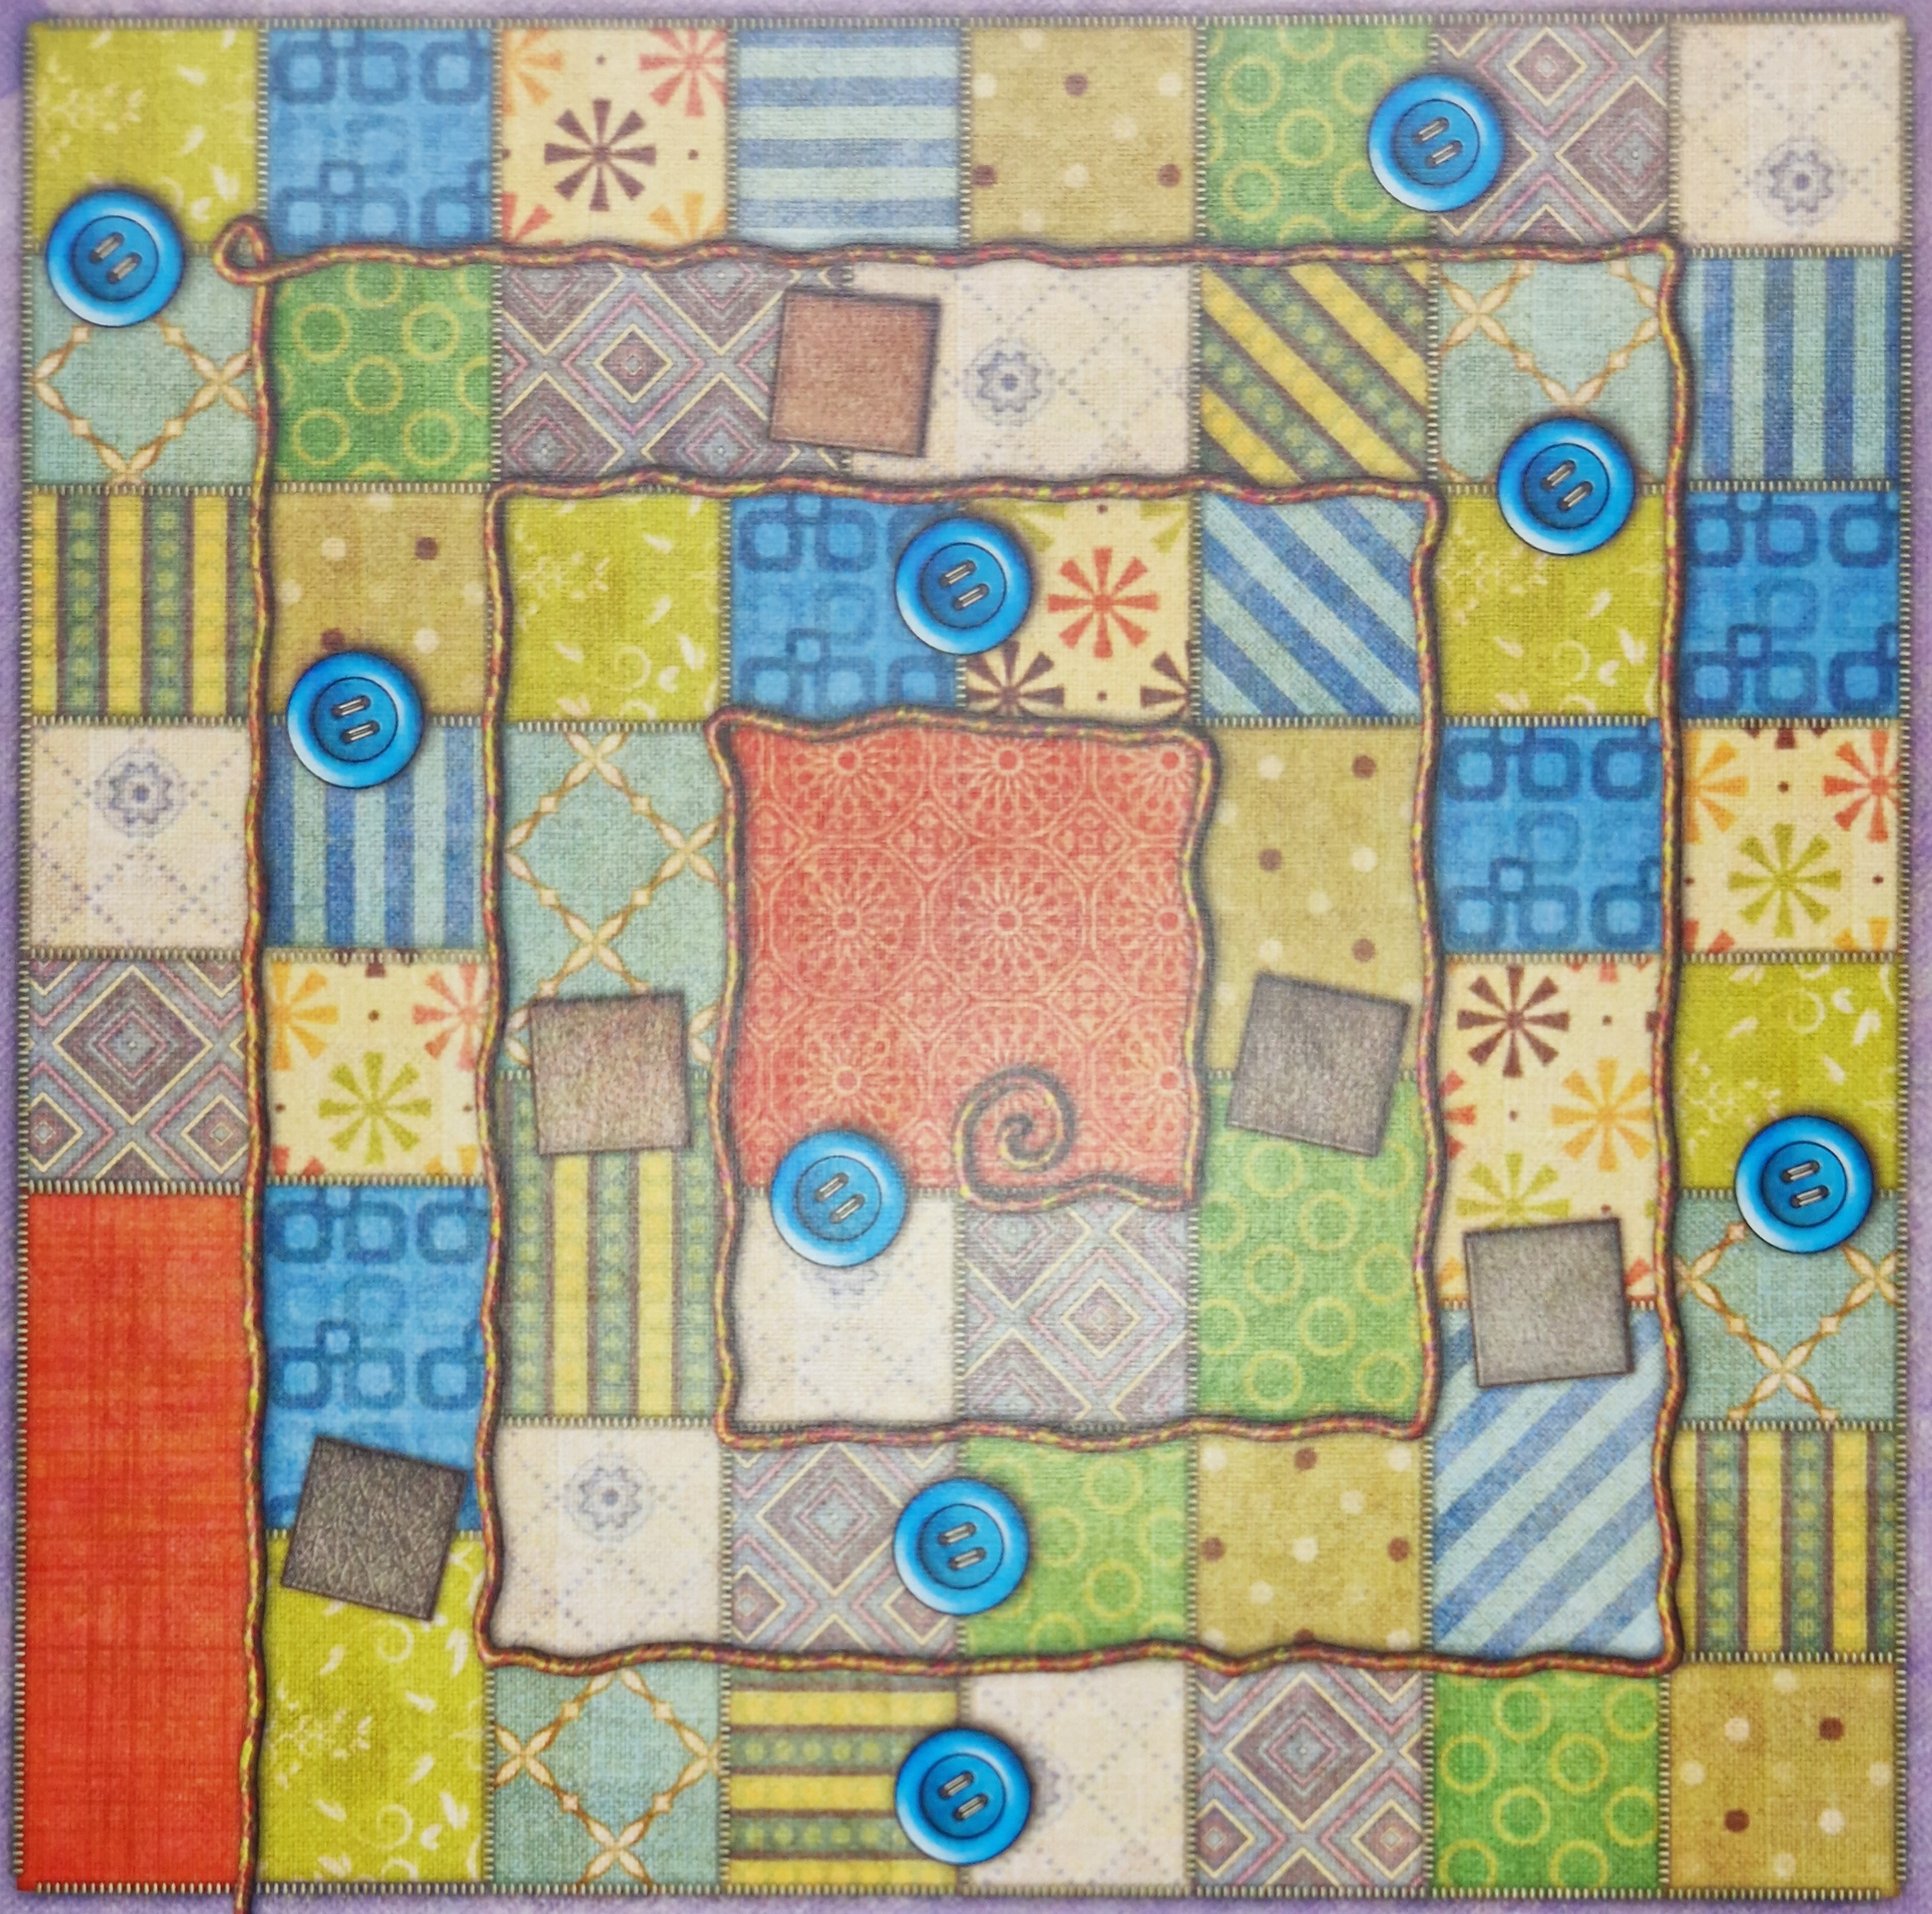
\includegraphics[width=0.625\textwidth]{res/pictures/assets/time-board-side-1.png}};
                                                                                       \drawshadow{image}
                                                                                   \end{tikzpicture}} &
        \adjustbox{center, width=0.4735\textwidth, valign=m, margin=0 1ex 0 0}{\begin{tikzpicture}
                                                                                       \node [inner sep=0pt,,outer sep=0pt,clip,rounded corners=0.15cm] (image) at (0,0) {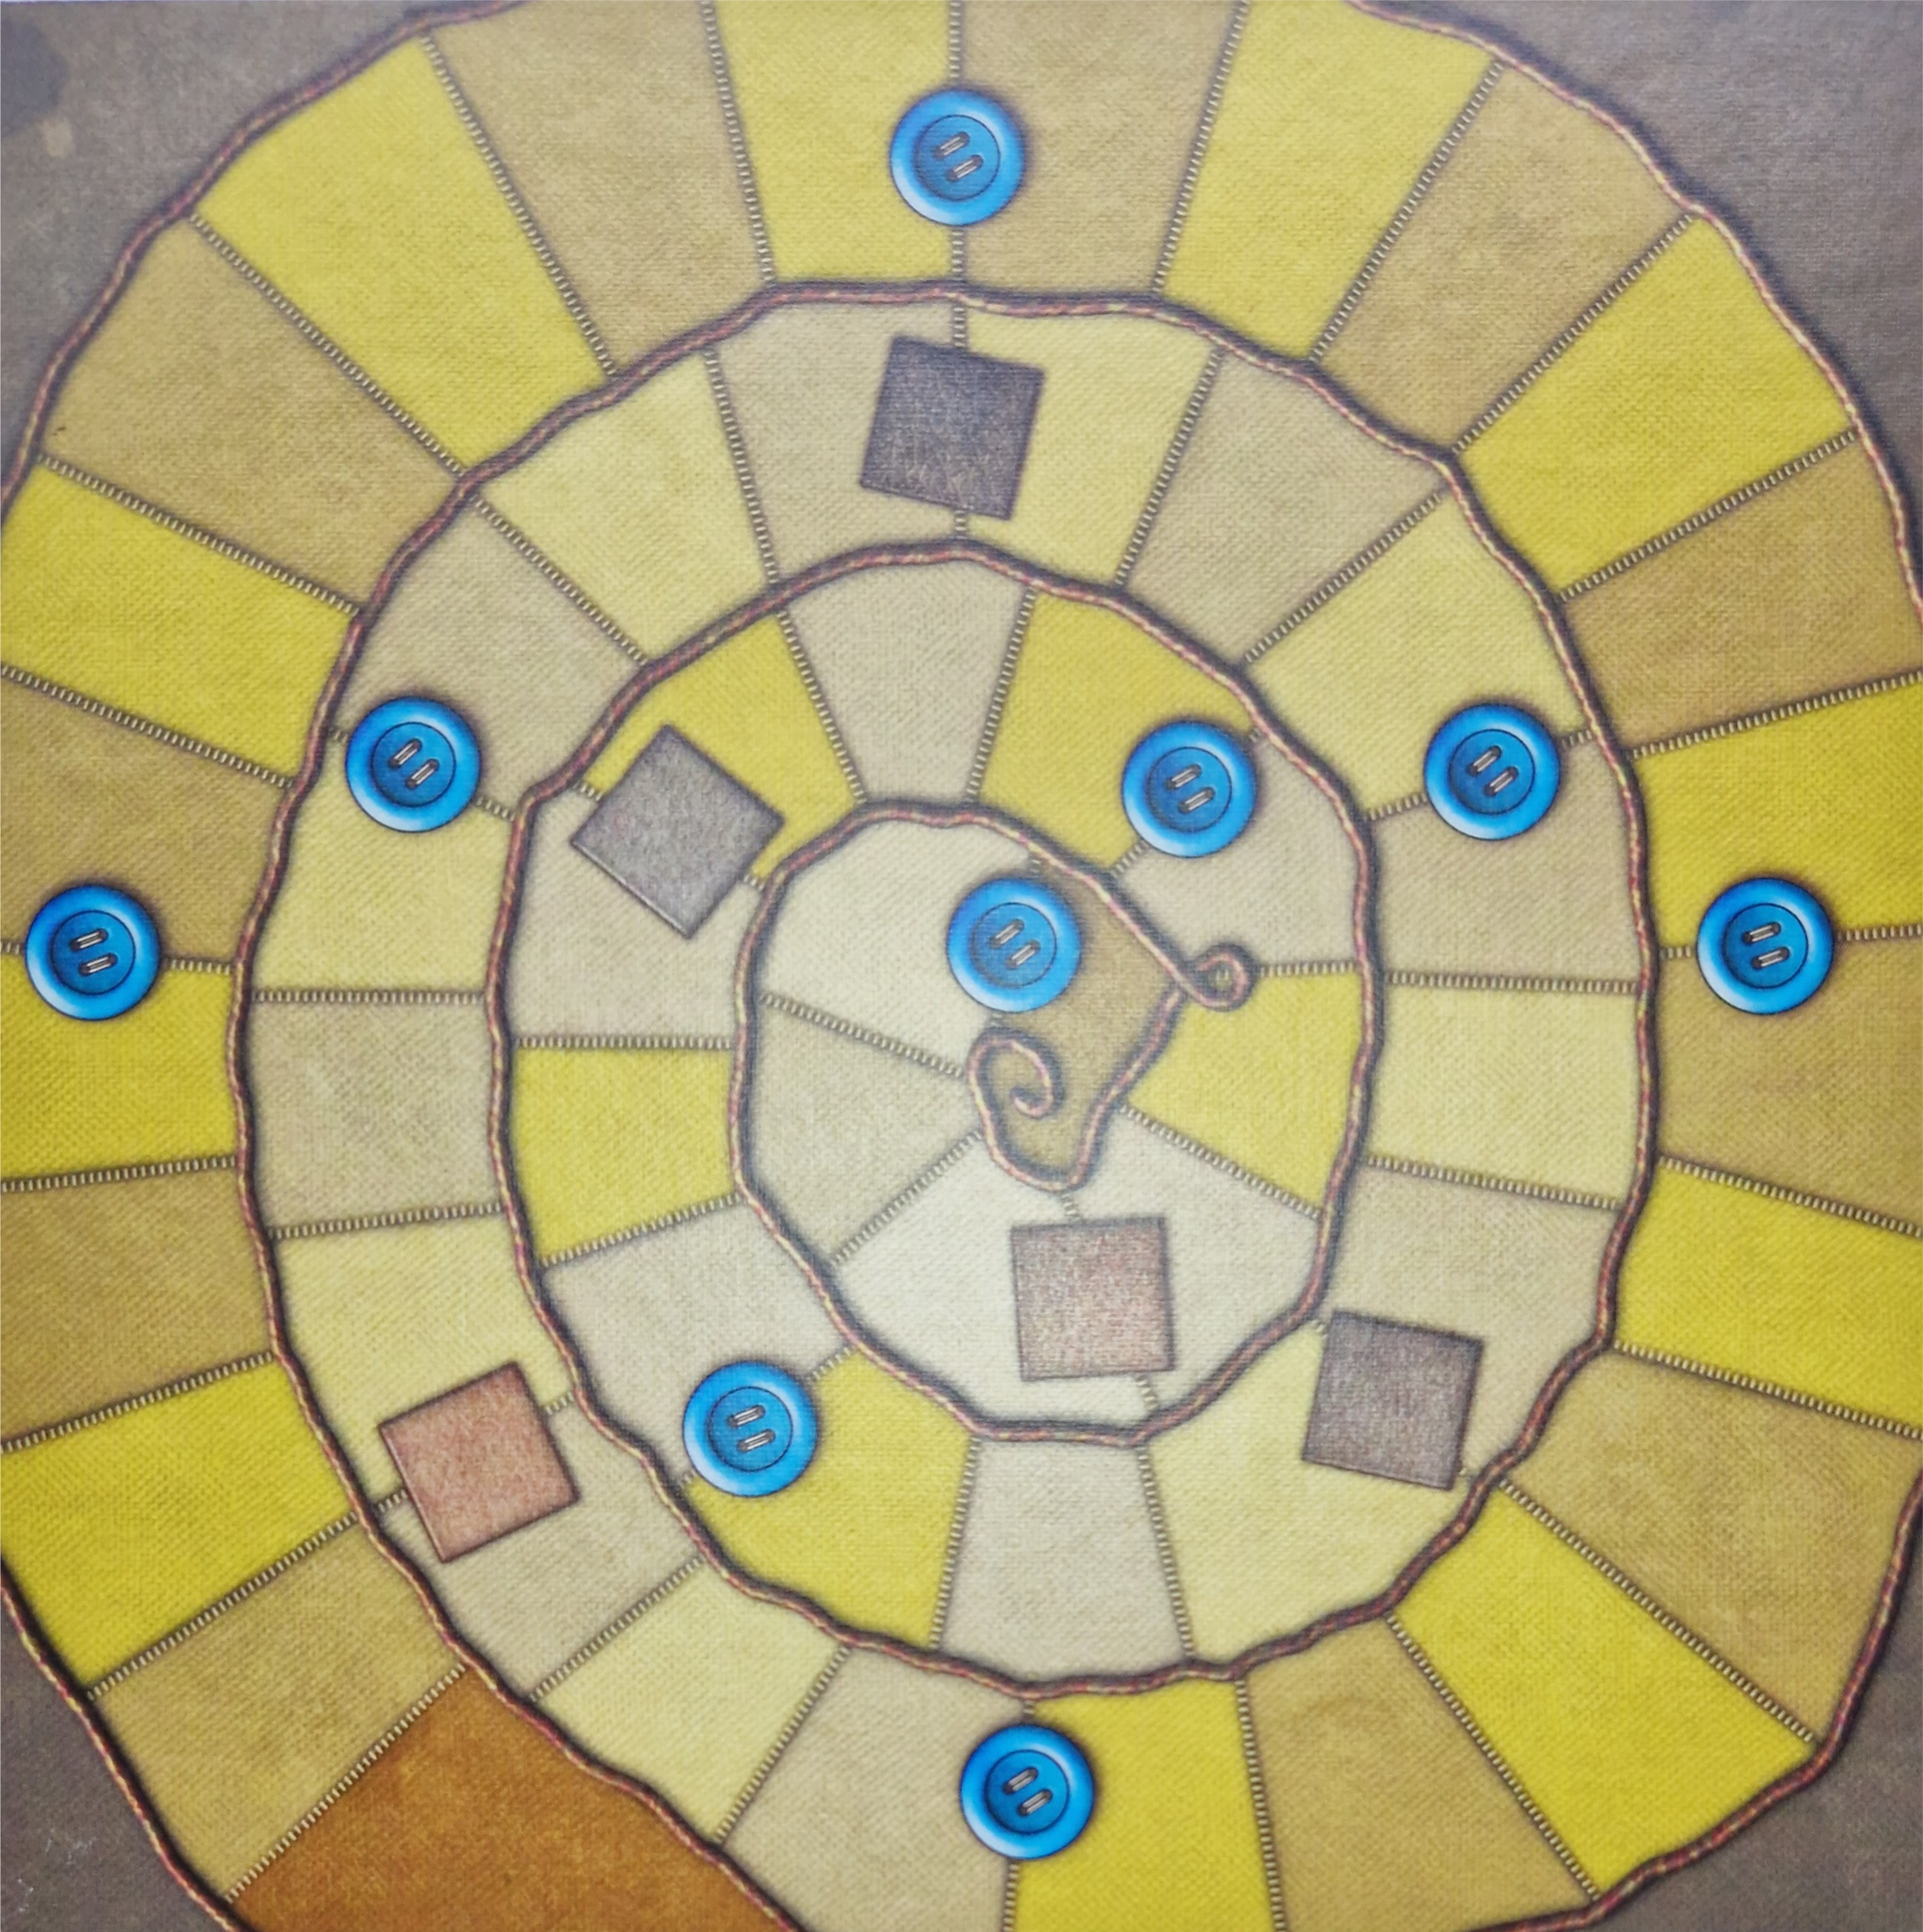
\includegraphics[width=0.625\textwidth]{res/pictures/assets/time-board-side-2.png}};
                                                                                       \drawshadow{image}
                                                                                   \end{tikzpicture}} \\
        \multicolumn{2}{c}{\adjustbox{valign=m, margin=0 2ex 0 2ex}{Zugrundeliegende Struktur des Zeitplans:}}                                                                            \\
        \multicolumn{2}{c}{\adjustbox{width=0.97\textwidth}{\includegraphics{res/pictures/time-board-structure.pdf}}}                                                                     \\
    \end{tabular}
    \vspace{5pt}
    \caption{Die Zeitpläne zusammen mit der zugrundeliegenden Struktur}
    \label{tabelle:isomorphie-zeitplan}
\end{table}

Aus diesem Grund kann Patchwork nachfolgend als ein Spiel betrachtet werden, da die Auswahl eines konkreten Zeitplans keinen Unterschied für die Betrachtung ausmacht.

\subsection*{Länge des Spiels}
\label{subsection:analyse-laenge-des-spiels}

In der Spieltheorie ist der Begriff eines Spielzuges nicht eindeutig. Ein Spielzug könnte eine einzelne Aktion eines Spielers sein, \zB das Auswählen und Legen eines Flickens in Patchwork von einem Spieler. Jedoch kann ein Spielzug auch so verstanden werden, dass beide Spieler eine Aktion machen müssen. So wird beispielsweise in rundenbasierten Spielen wie Schach ein Spielzug oft so angesehen, dass einmal die weiße und einmal die schwarze Seite gezogen haben müssen. Aufgrund dieser Zweideutigkeit wird ein Spielzug in der Spieltheorie mit einem \hyperref[text:ply]{\emph{Ply}} genauer definiert.

\begin{defStrich}[Ply]
    Ein Spielzug, welcher von einem Spieler gezogen wird, und stellt die kleinste mögliche Aktion in einem Spiel dar. \cite[S. 213]{1959.GameTheoryStudiesCheckers}
\end{defStrich}
\label{text:ply}
\vspace{-0.2cm}

Durch diese Definition kann genau definiert werden, was mögliche \hyperref[text:ply]{\emph{Plys}} in Patchwork sind. Die obige Definition für einen Spielzug, bei dem beide Spieler gezogen haben müssen, ist in Patchwork sowieso schwierig umzusetzen, da ein Spieler mehrere \hyperref[text:ply]{\emph{Plys}} hintereinander ausführen kann. Insgesamt gibt es drei mögliche Arten von \hyperref[text:ply]{\emph{Plys}} in Patchwork:

\begin{itemize}
    \item Vorrücken des Zeitsteins und Knöpfe erhalten
    \item Einen Flicken nehmen und auf dem Ablageplan platzieren
    \item Das Legen eines Spezialflicken auf den Ablageplan
\end{itemize}

Immer wenn ein Spieler an der Reihe ist, kann er zwischen dem Vorrücken und dem Platzieren von drei Flicken unterscheiden. Die Aktion einen Spezialflicken auf die Decke zu legen, kommt im Spiel immer genau fünfmal vor.

Patchwork endet, sobald beide Zeitsteine der Spieler das Zielfeld auf der Zeitleiste erreicht haben. Um ein möglichst langes Spiel zu spielen, muss also die Anzahl der Felder, die ein Spieler mit seinem Zeitstein pro \hyperref[text:ply]{\emph{Ply}} vorzieht, minimiert werden.

Für die Aktion \enquote{Einen Flicken nehmen und auf der Decke platzieren} ist die Anzahl der Felder immer durch den ausgewählten Flicken vorgegeben und beträgt mindestens 1 und maximal 6 (vgl. Zeitkosten in Anhang \ref{anhang:section-patchwork-patches}).

\pagebreak

Die Anzahl der Felder bei der Aktion \enquote{Vorrücken des Zeitsteins und Knöpfe erhalten} ist abhängig von der relativen Position der einzelnen Zeitsteine zueinander. Die maximale Anzahl an Feldern, die ein Zeitstein in einem Zug vorrücken kann, beträgt 7. Da immer ein Spielerwechsel stattfindet, sobald der Zeitstein des derzeitigen Spielers weiter vorrangeschritten ist als der Zeitstein des Gegners, muss für eine maximale Anzahl die Distanz zwischen den Zeitsteinen möglichst groß sein. Ein Zeitstein kann sich von dem anderem Zeitstein nur um maximal 6 Felder entfernen. Das ist der Fall, wenn ein Flicken mit Zeitkosten 6 ausgewählt wird, während sich beide Zeitsteine auf demselben Feld befinden. Nach dieser Aktion ist der andere Spieler an der Reihe, welche sein Zeitstein um 7 Felder fortbewegen kann (Distanz von 6 Feldern $+$ 1 Feld, um weiter vorrangeschritten zu sein als der andere Zeitstein). Die minimale Anzahl an Felder bei der Vorrücken-Aktion beträgt 1 und kann bei drei Spielzuständen auftreten. Zuerst ist es möglich, dass beide Zeitsteine auf demselben Feld sind, sodass der Spieler, welcher an der Reihe ist, seinen Zeitstein nur 1 Feld vorrückt. Weiterhin ist es möglich, dass ein Zeitstein auf dem Feld vor dem Ziel ist, während der andere Spieler bereits im Ziel ist. In dieser Situation darf der Zeitstein auch nur um ein Feld vorgerückt werden. Zuletzt existiert noch die Situation am Spielanfang. Da hier auch beide Zeitsteine auf demselben Feld \textemdash{} dem Startfeld des Zeitplans \textemdash{} sind, darf der Startspieler den Zeitstein auch nur um ein Feld vorrücken.

Um die Länge des Spiels zu maximieren, sollte jeder Spieler so wenige Felder wie möglich vorrücken. Nutzt jeder Spieler immer die \enquote{Vorrücken des Zeitsteins und Knöpfe erhalten} Aktion, so gibt es insgesamt 54 \hyperref[text:ply]{\emph{Plys}}, da auf dem Zeitplan insgesamt 53 Felder sowie ein Start- und ein Zielfeld existieren. Während beim ersten und letzen \hyperref[text:ply]{\emph{Ply}} der Erste bzw. Zweite Spieler seinen Zeitstein nur um 1 Feld vorrückt, muss der Zeitstein während des Spiels immer 2 Felder vorgerückt werden, da die vorherige Aktion \textemdash{} auch eine \enquote{Vorrücken des Zeitsteins und Knöpfe erhalten} Aktion \textemdash{} impliziert, dass der Zeitstein des Gegners genau 1 Feld vor dem eigenen Zeitstein liegt. Die Zeitkosten bei der Aktion \enquote{Einen Flicken nehmen und auf der Decke platzieren} sind immer fest, wobei es insgesamt neun Flicken gibt, bei denen die Zeitkosten auch 2 betragen. So können optimal 9 Vorrücken-Aktionen durch die Auswahl dieser Flicken ersetzt werden. Weiterhin gibt es aber auch noch die vier in \ref{tabelle:flicken-mit-zeitkosten-1} dargestellten Flicken, welche nur Zeitkosten von 1 besitzen. Wird nun ein Vorrücken-\hyperref[text:ply]{\emph{Ply}} mit 2 Zeitkosten durch eine Kombination aus Flicken mit Zeitkosten 1 auswählen und auf der Decke Platzieren und anschließend ein Vorrücken-\hyperref[text:ply]{\emph{Ply}} mit Zeitkosten 1 ersetzt, ist das Spiel um 4 weitere \hyperref[text:ply]{\emph{Plys}} verlängert.

\begin{table}[!ht]
    \centering
    \resizebox{\textwidth}{!}{
        \begin{tabular}[t]{c|c|c|c}
            \adjustbox{valign=t, raise=-16.25ex}{\includegraphics[width=0.2\textwidth]{res/pictures/assets/00-front.png}} &
            \adjustbox{valign=t, raise=0ex}{\includegraphics[width=0.3\textwidth]{res/pictures/assets/06-front.png}}      &
            \adjustbox{valign=t, raise=-9.05ex}{\includegraphics[width=0.2\textwidth]{res/pictures/assets/21-front.png}}  &
            \adjustbox{valign=t, raise=-16.25ex}{\includegraphics[width=0.5\textwidth]{res/pictures/assets/27-front.png}}   \\
        \end{tabular}
    }
    \vspace{5pt}
    \caption{Die vier Flicken mit Zeitkosten 1}
    \label{tabelle:flicken-mit-zeitkosten-1}
    \vspace*{-0.35cm}
\end{table}

Das ist möglich, da wie oben beschrieben der Zeitstein des derzeitigen Spielers immer direkt hinter dem Zeitstein des Gegners ist. Wird nun ein Flicken mit Zeitkosten 1 ausgewählt, befindet sich der Zeitstein des derzeitigen Spielers auf dem Zeitstein des Gegners. So kann ein Vorrücken-\hyperref[text:ply]{\emph{Ply}} mit Zeitkosten von 1 anstatt 2 ausgeführt werden. Da alle anderen Flicken höhere Zeitkosten verlangen, ist keine weitere Optimierung des Spiels hinsichtlich der der maximalen Länge mehr möglich.

Die maximale Länge des Brettspiels ergibt sich somit aus der Kombination der 54 Vorrücken-\hyperref[text:ply]{\emph{Plys}} zusammen mit den 4 zusätzlich gewonnenen \hyperref[text:ply]{\emph{Plys}} durch das Legen von Flicken mit Zeitkosten 1. Weiterhin kommen noch die fünf \hyperref[text:ply]{\emph{Plys}} für das Legen von Spezialflicken hinzu. Somit beträgt die maximale Länge von Patchwork \textbf{63} \hyperref[text:ply]{\emph{Plys}}.

\subsection*{Maximale Anzahl aufeinanderfolgender \hyperref[text:ply]{Plys} eines Spielers}

Neben der Gesamtlänge des Spiels kann auch betrachtet werden, wie oft ein Spieler maximal hintereinander ziehen kann. Wie oben erläutert, kann der Zeitstein des Gegners maximal 6 Felder vor dem eigenen Zeitstein liegen. Zuerst können in 4 \hyperref[text:ply]{Plys} die vier Flicken mit Zeitkosten 1 genommen und platziert werden. Danach kann noch ein Flicken mit Zeitkosten 2 erworben werden, sodass sich der Zeitstein auf demselben Feld wie der Gegner befindet. In einem weiteren \hyperref[text:ply]{Ply} kann der Spieler noch durch laufen bzw. Flicken platzieren an dem Gegner vorbeiziehen. Zuletzt ist es möglich, dass der Spieler dabei einen Spezialflicken passiert und diesen in einem weiteren \hyperref[text:ply]{Ply} legen muss\footnote{Da der Spieler maximal 6 Felder auf dem Zeitplan auf einmal vorrücken kann, ist es nicht möglich 2 Spezialflicken zu passieren, da diese auch immer genau 6 Felder voneinander entfernt sind.}. Somit kann ein Spieler maximal \textbf{7} \hyperref[text:ply]{Plys} hintereinander ausführen.

\subsection*{Minimum und Maximum für die Anzahl an möglichen Aktionen}

Um die Komplexität von Patchwork zu untersuchen, ist es auch interessant zu betrachten, wie viele Auswahlmöglichkeiten einem Spieler bei seinem Zug zur Verfügung stehen.

Ist ein Spieler am Zug, kann er immer die Aktion \enquote{Vorrücken des Zeitsteins und Knöpfe erhalten} auswählen. Somit beträgt die minimale Anzahl an Aktionen mindestens 1. Dabei handelt es sich auch um das Minimum, da der derzeitige Spieler weniger Knöpfe in seinem Vorrat haben kann, als jede der ersten 3 Flicken nach der Spielfigur an Knöpfen kostet. Somit kann der Spieler sich keinen der Flicken leisten und muss automatisch seinen Zeitstein vorrücken.

Eine obere Schranke für die maximal mögliche Anzahl an Aktionen ergibt sich als:

\vspace*{-0.45cm}
\begin{equation}
    \text{Obere Schranke}_{\text{Aktionen}} = \:
    \underset{\mathclap{\substack{\rotatebox[origin=c]{90}{\(\{ \)} \mathstrut \\ \text{Vorrücken}}}}{1}
    + \:
    \overset{\mathclap{\substack{\text{maximale Auswahlanzahl} \mathstrut \\ \text{Flicken} \mathstrut \\ \rotatebox[origin=c]{-90}{\(\{ \)}}}}{3} \:
    \times \:
    \max\limits_{\mathclap{\substack{\phantom{\text{\tiny m}} \\ f\, \in\, \text{Flicken}}}} \:\,
    \left\lvert\, \text{Platziermöglichkeiten}\left( f \right)\, \right\rvert
\end{equation}
\vspace*{-0.15cm}

Dabei ist eine $+1$ für die Aktion \enquote{Vorrücken des Zeitsteins und Knöpfe erhalten} vorhanden. Weiterhin gibt es für einen Spieler die Möglichkeit aus maximal 3 Flicken einen Flicken auszuwählen. Diese Anzahl wird multipliziert mit der maximalen Anzahl an Möglichkeiten, mit dem ein Flicken auf dem Ablageplatz platziert werden kann.

Um die maximale Anzahl an Platzierungsmöglichkeiten festzulegen, muss zuerst betrachtet werden, auf wie viele Arten ein Flicken auf die Ablagedecke gelegt werden kann. Die Operationen, welche vor dem Platzieren auf einen Flicken angewendet werden können, sind Drehungen und Spiegelungen, wodurch die Flicken identisch zur Diedergruppe $D_4$ sind. Die Gruppe besteht aus 8 Elementen \cite[S. 33]{2015.AbstractAlgebra}, was somit gleichzeigt die maximale Anzahl an Transformationen für ein Flicken ist. Jedoch muss beachtet werden, dass die Flicken die maximale Anzahl nicht erreichen müssen. Zum Beispiel existiert ein $2\times2$ Flicken, welcher im Sinne der Diedergruppe 8 Ausprägungen besitzt, jedoch auf der Ablagedecke mit allen Drehungen und Spiegelungen immer genau dieselben Felder bedeckt. Für die maximale Platzierungsanzahl ist aber nur relevant, dass ein Flicken existiert, welcher bei allen 8 Transformationen eine andere Anordnung aufweist. Dieser Flicken existiert und ist in Abbildung \ref{fig:diedergruppe} dargestellt.

\pagebreak

\vspace*{-0.85cm}
\begin{figure}[!ht]
    \centering
    \includegraphics[width=0.835\textwidth]{res/pictures/dihedral-group.png}
    \vspace*{-0.23cm}
    \caption{Flicken mit 8 verschiedenen Transformationen}
    \label{fig:diedergruppe}
    \vspace*{-0.22cm}
\end{figure}

Weiterhin gibt es verschiedene Möglichkeiten den transformierten Flicken auf den $9\times9$ Felder großen Ablageplan zu legen. Die Möglichkeiten lassen sich dabei einfach wie in Term \ref{eqn:ablagefeld-platzierungen} in Abhängigkeit von der Breite und Höhe des Flickens sowie der Anzahl der unterschiedlichen Transformationen berechnen.

\vspace*{-0.28cm}
\vspace*{-0.4cm}
\begin{equation}
    \label{eqn:ablagefeld-platzierungen}
    \left( 9 - \text{Höhe}  + 1 \right) \cdot
    \left( 9 - \text{Breite} + 1 \right) \cdot
    \left\lvert\, \text{Transformationen} \,\right\rvert
    \vspace*{-0.28cm}
\end{equation}

Die Anzahl der Platzierungsmöglichkeiten für den in \ref{fig:diedergruppe} dargestellten $3\times 2$ großen Flicken beträgt somit $\left( 9 - 3 + 1 \right) \cdot \left( 9 - 2 + 1 \right) \cdot 8 = 448$. Jedoch muss für die Platzierungsmöglichkeiten beachtet werden, dass sich die Anzahl reduziert, je größer ein Flicken ist. Somit muss für alle Flicken, dessen Höhe $\le 3$ und Breite $\le 2$ ist \textemdash{} wobei mindestens eine der beiden Ungleichungen strikt (also $<$) sein muss \textemdash{} überprüft werden, ob mehr Platzierungsmöglichkeiten bestehen als bei dem Flicken von \ref{fig:diedergruppe}. Es existieren nur 3 Flicken dieser Art, welche in Tabelle \ref{tabelle:kleine-flicken} dargestellt sind. Jeder dieser Flicken weißt dabei durch die geringere Anzahl an verschiedenen Transformationsmöglichkeiten insgesamt weniger Platzierungsmöglichkeiten auf als der Flicken in \ref{fig:diedergruppe}.

\vspace*{-0.35cm}
\begin{table}[!ht]
    \centering
    \begin{tabular}[t]{c|c|c|c}
        \raisebox{0pt}[0.35ex][0.35ex]{Flicken} & \adjustbox{valign=m}{\includegraphics[width=0.1525\textwidth]{res/pictures/assets/00-front.png}} & \adjustbox{valign=m}{\includegraphics[width=0.1525\textwidth]{res/pictures/assets/09-front.png}} & \adjustbox{valign=m}{\includegraphics[width=0.1525\textwidth]{res/pictures/assets/21-front.png}} \\ \hline
        \makecell{Platzierungs-                                                                                                                                                                                                                                                                                                                          \\möglichkeiten} & $9 \cdot 8 \cdot 2 = 144$                                                                      & $8 \cdot 8 \cdot 1 = 64$                                                                       & $8 \cdot 8 \cdot 4 = 256$                                                                      \\
    \end{tabular}
    \vspace{2pt}
    \caption{Platzierungsmöglichkeiten der kleineren Flicken}
    \label{tabelle:kleine-flicken}
\end{table}
\vspace*{-4.5cm}

\pagebreak

\begin{wrapfigure}{r}{0.25\textwidth}
    \vspace*{-0.1cm}
    \centering
    \includegraphics[width=0.12\textwidth]{res/pictures/assets/08-front.png}

    \includegraphics[width=0.12\textwidth]{res/pictures/assets/14-front.png}

    \includegraphics[width=0.18\textwidth]{res/pictures/assets/19-front.png}
    % \vspace{-10pt}
    % Das folgende ist ein Trick, um "Abbilgung x.y" in eine
    % eigene Zeile zu packen. Der Text zwischen [ und ] steht
    % im Abbildungsverzeichnis. Der Text darunter wird
    % tatsächlich angezeigt.
    \caption[Alle Flicken mit 448 Platzierungsmöglichkeiten]{\unskip}
    Alle Flicken mit 448 Platzierungsmöglichkeiten
    \label{fig:flicken-mit-448}
    \vspace*{-0.1cm}
\end{wrapfigure}

Um sicherzustellen, dass die maximale Platzierungsmöglichkeit auf dem Ablageplan auch tatsächlich für die drei zur Verfügung stehenden Flicken auftreten kann, müssen mindestens drei unterschiedliche Flicken mit einer Größe von $3 \times 2$ bzw. $2 \times 3$ existieren, welche 448 Möglichkeiten zur Platzierung auf dem Ablageplan besitzen. Das ist der Fall, wie die Flicken in Abbildung \ref{fig:flicken-mit-448} zeigen.

Um die maximale Anzahl an möglichen Aktionen festzustellen, muss zuletzt noch das Platzieren von Spezialflicken als Sonderfall betrachtet werden. Da alle Spezialflicken eine Größe von $1 \times 1$ besitzen, unterscheiden sich die Transformationen nicht hinsichtlich der Platzierung auf dem Ablageplan. Somit gibt es $9 \cdot 9 \cdot 1 = 81$ mögliche Aktionen einen Spezialflicken auf dem Ablageplan zu platzieren.

Das tatsächliche Maximum für die mögliche Anzahl an Aktionen ergibt sich dann als das Maximum der normalen Aktionen und der Aktion \enquote{Legen eines Spezialflicken} wie in \ref{eqn:max-aktionen} dargestellt ist:

\vspace*{-0.4cm}
\begin{equation}
    \label{eqn:max-aktionen}
    \text{Maximum}_{\text{Aktionen}} = \max \left\{ 1 + 3 \cdot 448\, ,\, 81 \right\} = 1345
\end{equation}

Dabei ist anzumerken, dass die maximale Anzahl an Platzierungsmöglichkeiten für normale sowie Spezialflicken nur genau dann möglich ist, wenn der Ablageplan noch leer ist. Weiterhin kann die maximale Auswahlmöglichkeit auch bereits direkt am Anfang des Spiels geschehen, da alle Flicken in \ref{fig:flicken-mit-448} mit dem Startbudget von 5 Knöpfen gekauft werden können.

\subsection*{Obere und untere Schranke für die Wertung eines Spielers}

In dieser Sektion wird eine obere und eine untere Schranke für die Wertung eines Spielers am Ende des Spiels festgesetzt. Da sich die Wertung aus dem am Ende vorhandenen Vorrat an Knopf-Plättchen und der Anzahl der Lücken im eigenen Spielbrett zusammensetzt, werden zunächst die maximal möglichen Werte für diese beiden Komponenten bestimmt. Anschließend werden die Schranken für die Wertung eines Spielers am Ende des Spiels festgesetzt.

% Reference for this paragraph: /code/patchwork/transposition_table/src/zobrist_hash.rs

Ein Spieler hat 2 Möglichkeiten bei der Wertung möglichst viele positive Punkte zu sammeln. Erstens kann der Spieler das $7 \times 7$ Sonderplättchen erhalten, was die Wertung um 7 Punkte erhöht. Weiterhin zählt jeder Knopf in seinem Vorrat einen Punkt. Zu Beginn erhält jeder Spieler 5 Knöpfe. Der Knopfvorrat kann nur durch die 9 Knopf-Wertungen auf der Zeitleiste erhöht werden. Dabei ist die Erhöhung des Knopfvorrates abhängig von den Flicken auf dem Ablageplan. Da der Ablageplan eine feste Größe besitzt, existiert somit auch eine Obergrenze für das zusätzliche Knopfeinkommen und die Anzahl der positiven Punkte für die Wertung ist von oben begrenzt. Die einfache Obergrenze für den positiven Anteil bei der Endbewertung ist daher $5+7+81\cdot 9=741$.

Diese Obergrenze würde aber erfordern, dass alle Flicken auf dem Ablageplan mindestens die gleiche Anzahl an Knopfeinkommen haben, wie die Anzahl der Felder, die sie bedecken. Diese Annahme gilt für keinen der Flicken in Patchwork. Für eine realistischere Obergrenze werden alle Flicken nach dem prozentualen Anteil des Knöpfeinkommens im Verhältnis zur Anzahl der Felder, die sie bedecken, sortiert (Siehe Anhang \ref{anhang:section-patchwork-patches}). Werden nun alle Flicken ausgewählt, bis die Grenze von 81 kombinierten Feldern erreicht ist, ergibt sich eine neue Obergrenze für das maximale Knopfeinkommen durch den Ablageplan von 32. Eine beispielhafte Anordnung dieser Flicken ist in Abbildung \ref{fig:quilt-board-max-button-income} zu sehen. Dabei bleiben 2 Felder auf dem Ablageplan frei. Jedoch können alle Flicken mit 2 oder weniger Feldern kein Knopfeinkommen generieren, wodurch dies kein Problem darstellt.

\begin{figure}[!ht]
    \centering
    \begin{minipage}{.48\textwidth}
        \centering
        \begin{tikzpicture}
            \node [inner sep=0pt,,outer sep=0pt,clip,rounded corners=0.15cm] (image) at (0,0) {\includegraphics[width=0.765\linewidth]{res/pictures/max-button-income.jpg}};
            \drawshadow{image}
        \end{tikzpicture}
        \captionsetup{format=plain, singlelinecheck=false}
        \setcapindent{0pt}
        \caption[Anordnung von Flicken mit einem Knopfeinkommen von 32]{Anordnung von Flicken mit einem Knopfeinkommen von 32 \\ \phantom{und Zeitkosten von 66}}
        \label{fig:quilt-board-max-button-income}
    \end{minipage}
    \hfill
    \begin{minipage}{.48\textwidth}
        \centering
        \begin{tikzpicture}
            \node [inner sep=0pt,,outer sep=0pt,clip,rounded corners=0.15cm] (image) at (0,0) {\includegraphics[width=0.765\linewidth]{res/pictures/real-max-button-income.jpg}};
            \drawshadow{image}
        \end{tikzpicture}
        \captionsetup{format=plain, singlelinecheck=false}
        \setcapindent{0pt}
        \caption[Anordnung von Flicken mit Zeitkosten von 58]{Anordnung von Flicken mit einem Knopfeinkommen von 30 \\ und Zeitkosten von 58}
        \label{fig:quilt-board-real-max-button-income}
    \end{minipage}
\end{figure}

Jedoch betragen die benötigten Zeitkosten bei dieser Anordnung $66$, wodurch diese Anordnung im tatsächlichen Spiel nicht auftreten kann. Aus diesem Grund muss für die Bewertung eines Flickens noch die benötigte Zeit wie in Term \ref{eqn:patch-value-for-max-button-income} einfließen.

\begin{equation}
    \label{eqn:patch-value-for-max-button-income}
    \frac{\text{Knopfeinkommen}}{\text{Felder}\, \cdot\, \text{Zeitkosten}}
\end{equation}

Somit ergibt sich eine neue Sortierung und Anordnung der Flicken auf dem Ablageplan, wie in Abbildung \ref{fig:quilt-board-real-max-button-income}. Das maximale Knopfeinkommen beträgt dabei $30$ Knöpfe und die benötigte Zeit beträgt $58$. Auf dem Zeitplan selbst, existieren nur $54$ Felder. Ein Spieler kann aber auf dem letzten Feld vor dem Ziel noch einen Flicken nehmen und läuft \emph{immer genau $1$} Feld. Somit kann der Spieler hier auch ein Flicken mit den maximalen Zeitkosten von $6$ nehmen. Da $58 - 6 = 52 < 54$ ist die Anordnung in \ref{fig:quilt-board-real-max-button-income} also auch tatsächlich während des Spiels erreichbar. Eine obere Schranke für das Knopfeinkommen durch den Ablageplan im gesamten Spiel ist somit die Anzahl der Knopf-Wertungen auf dem Zeitplan ($9$) multipliziert mit dem maximalen Knopfeinkommen pro Knopf-Wertung ($30$) $= 270$.

Der Spieler bekommt bei der Wertung am Ende nur Punkte abgezogen, wenn nicht alle Felder auf seinem Ablageplan bedeckt sind. Es gibt mehrere Möglichkeiten solch einen vollen Ablageplan im Spielverlauf zu erhalten (ein Beispiel hierfür ist in Anhang \ref{anhang:section-ablageplan-81} zu sehen). Somit kann für eine Obergrenze bei der Wertung mit einem Punktabzug von 0 gerechnet werden. Zusammen mit dem Ablageplan von \ref{fig:quilt-board-real-max-button-income} würde sich somit mit $5 + 7 + 30 \cdot 9 - 0 = \boldsymbol{282}$ eine neue Obergrenze für die maximale Wertung eines Spielers ergeben.

Nun kann sich der minimal erreichbaren Wertung eines Spielers zugewendet werden. Eine sehr einfache Untergrenze für die minimale Wertung eines Spielers ist $-162$, \dash ein leerer Ablageplan und 0 Knöpfe im Knopfvorrat. Diese Wertung kann jedoch offensichtlich nicht erreicht werden, da die einzige Möglichkeit Knöpfe aus dem Vorrat abzugeben gleichzeitig darin besteht, den Ablageplan zu füllen und jeder Spieler mit mindestens 5 Knöpfen startet.

Aus der einfachen Abschätzung lässt sich leicht erkennen, dass jeder Spieler mit einer Wertung von $5 - 2 * 81 = -157$ startet. Nun kann für jede Aktion eine Value-Funktion $V_{\alpha}\left(A\right)$ definiert werden, die aufzeigt, wie sich dieser Startwert durch die Aktion ändert. Um die minimale Wertung am Ende zu erreichen, muss nun die Summe aller im Spiel getätigten Aktionen wie in \ref{eqn:patch-value-minimize-objective} minimiert werden.

\begin{align}
    \label{eqn:patch-value-minimize-objective}
    \operatorname{minimiere} \sum V\left(A\right)
\end{align}

Die Value-Funktion für \enquote{Vorrücken und Knöpfe erhalten} ist für ein Feld immer Konstant $V(Walk) = 1$, \dash jede Vorrücken-Aktion erhöht zwangsweise das Endergebnis um 1.

Auch für die Aktion \enquote{Flicken nehmen und einfügen} lässt sich die Value-Funktion definieren. Diese hängt von mehreren Faktoren ab. Zuerst wird die Endwertung für jedes bedeckte Feld um 2 erhöht. Weiterhin wird die Endwertung um die Knopfkosten des Flickens verringert. Zuletzt muss noch das Knopfeinkommen auf die Wertung addiert werden. Dieses hängt dabei von einem Parameter $\alpha$ ab, was die Anzahl der noch ausstehenden Knopf-Wertungen auf dem Zeitplan darstellt. Da sich die letzte Knopf-Wertung direkt vor dem Ziel befindet, ist $\alpha$ immer größer gleich 1.Die Value-Funktion für Flicken ist in Gleichung \ref{eqn:patch-value-for-min-value} abgebildet.

\vspace*{-0.2cm}
\begin{align}
    \label{eqn:patch-value-for-min-value}
    V_{\alpha}\left(F\right) = 2 \cdot Felder_F - \text{Knopfkosten}_F + \text{Knopfeinkommen}_F \cdot \alpha
    \intertext{\begin{flushright} \vspace*{-1.25cm} wobei $\alpha \ge 1$ die Anzahl der noch ausstehenden Knopf-Wertungen ist \end{flushright}} \vspace*{-1cm} \notag
\end{align}
\vspace*{-2.2cm}

\begin{wrapfigure}{r}{0.21\textwidth}
    \vspace*{-0.5cm}
    \centering
    \includegraphics[width=0.2\textwidth]{res/pictures/assets/04-front.png}
    \vspace{-10pt}
    % Das folgende ist ein Trick, um "Abbilgung x.y" in eine
    % eigene Zeile zu packen. Der Text zwischen [ und ] steht
    % im Abbildungsverzeichnis. Der Text darunter wird
    % tatsächlich angezeigt.
    \caption[Flicken mit $V_1\left(F\right) = -2$]{\unskip}
    Flicken mit $V_1\left(F\right) = -2$
    \label{fig:negative-value-patch}
    \vspace*{-0.375cm}
\end{wrapfigure}

Nach Einsetzen aller Flicken in die Value-Funktion ergeben sich für alle Flicken und alle $\alpha > 1$ im Vergleich zu der Laufen-Aktion Werte größer gleicht 1. Somit sind alle \enquote{Flicken nehmen und einfügen} Aktionen vor der vorletzten Knopf-Wertung äquivalent oder öfters der Fall besser als \enquote{Vorrücken und Knöpfe erhalten}. Für $\alpha = 1$ gibt es für den Vergleich $ V_1\left(F\right) - V\left(Walk\right)$ insgesamt 6 Flicken mit dem Ergebnis $\le 0$. Somit kann kurz vor dem Ziel ein Flicken gekauft werden, mit dem Resultat, dass das Endergebnis schlechter ausfällt als nur zu laufen. Da die Summe der Zeitkosten von je 2 dieser 6 Flicken größer als 6 ist, kann jedoch nur genau einer dieser Flicken gekauft werden. Dabei muss darauf geachtet werden, dass auf dem Zeitplan auch genauso viele Felder gelaufen werden, wie der Flicken vorgibt und keine Zeitkosten mit in das Ziel genommen werden. Der in Abbildung \ref{fig:negative-value-patch} dargestellte Flicken besitzt als einziger der Sechs eine Value-Funktion von $-2$ bei $\alpha = 1$ und minimiert somit die Endwertung.

Für Spezialflicken ist die Value-Funktion Konstant $V\left(\text{Spezialflicken}\right) = 2$, da immer genau ein Feld auf dem Ablageplan befüllt wird. Da sich die Wertung somit durch einen Spezialflicken erhöhen würde, sollten für die minimale Wertung keine Spezialflicken eingesammelt werden.

Um nun die minimale Wertung am Ende zu erhalten kann ein Spieler also 47-mal hintereinander laufen und zuletzt den in \ref{fig:negative-value-patch} dargestellten Flicken kaufen. Dadurch ergibt sich für die minimale Wertung am Ende des Spiels eine Wertung von $5 - 2 \cdot 81 + 47 - 7 + 2 \cdot 4 + 3 = \boldsymbol{-106}$ Punkten. Im Gegensatz dazu bringt ein Spielverlauf, bei dem ein Spieler nur läuft eine Endwertung ovn $-104$ Punkten.

\subsection*{Maximale Wertung als Optimierungsproblem}

Die Schätzung im vorherigen Abschnitt für die maximale Wertung eines Spielers ist an einigen Stellen problematisch. Das größte Problem ist hierbei, dass angenommen wird, dass der Ablageplan bereits bei der ersten Knopf-Wertung komplett befüllt ist und somit das maximalen Knopfeinkommen von $30$ generiert. Somit handelt es sich bei der Obergrenze um eine viel zu große Schätzung. Um einen exakten Wert für die maximale Knopfwertung am Ende eines Spiels zu erhalten, kann das Problem als ein \ac{ILP}-Optimierungsproblem formuliert werden. Im ersten Schritt werden dazu für das Problem relevante Konstanten und Variablen definiert. Diese werden anschließend zur Definition der zu maximierenden Zielfunktion, sowie den Ungleichungen, welche erfüllt sein müssen, verwendet. Zuletzt kann das lineare Optimierungsproblem mit einem Programm gelöst werden.

\textbf{Konstanten}

Nachfolgend fünf für die maximalen Wertung in Patchwork relevante Konstanten. Die ersten vier Konstanten bilden dabei für jeden Flicken in Patchwork genau einen Wert ab. Als bijektive Abbildung zwischen Flicken und Zeile wird dabei die Tabelle in Anhang \ref{anhang:section-patchwork-patches} verwendet.

\renewcommand{\arraystretch}{0.6666}

\begin{addmargin}[1em]{0em}
    Knopfkosten der Flicken (\emph{cost}) \vspace*{-10pt}
    \begin{fleqn}
        \begin{align*}
            \begingroup
            \setlength\arraycolsep{1.5pt}
            c = \begin{bmatrix}
                    2 & 10 & 5 & 8 & 7 & 4 & 2 & 2 & 2 & 6 & 2 & 1 & 7 & 10 & 4 & 7 & 1 & 5 & 10 & 4 & 1 & 1 & 1 & 3 & 2 & 2 & 3 & 7 & 3 & 5 & 3 & 3 & 0
                \end{bmatrix}^\mathsf{T}
            \endgroup \in \mathbb{N}_0^{33} &
        \end{align*}
    \end{fleqn}
    Zeitkosten der Flicken (\emph{time}) \vspace*{-10pt}
    \begin{fleqn}
        \begin{align*}
            \begingroup
            \setlength\arraycolsep{1.5pt}
            t = \begin{bmatrix}
                    1 & 4 & 3 & 6 & 6 & 2 & 1 & 3 & 2 & 5 & 3 & 2 & 2 & 5 & 6 & 4 & 5 & 4 & 3 & 2 & 4 & 3 & 2 & 1 & 2 & 2 & 2 & 1 & 3 & 5 & 6 & 4 & 3
                \end{bmatrix}^\mathsf{T}
            \endgroup \in \mathbb{N}^{33}
        \end{align*}
    \end{fleqn}
    Knopfeinkommen der Flicken (\emph{profit}) \vspace*{-10pt}
    \begin{fleqn}
        \begin{align*}
            \begingroup
            \setlength\arraycolsep{1.5pt}
            p = \begin{bmatrix}
                    0 & 3 & 1 & 3 & 3 & 0 & 0 & 0 & 0 & 2 & 1 & 0 & 2 & 3 & 2 & 2 & 1 & 2 & 2 & 1 & 1 & 0 & 0 & 0 & 0 & 0 & 1 & 1 & 1 & 2 & 2 & 1 & 1
                \end{bmatrix}^\mathsf{T}
            \endgroup \in \mathbb{N}_0^{33}
        \end{align*}
    \end{fleqn}
    Fläche der Flicken (\emph{area}) \vspace*{-10pt}
    \begin{fleqn}
        \begin{align*}
            \begingroup
            \setlength\arraycolsep{1.5pt}
            a = \begin{bmatrix}
                    2 & 5 & 8 & 6 & 4 & 6 & 6 & 7 & 5 & 4 & 5 & 6 & 6 & 6 & 4 & 6 & 6 & 5 & 5 & 4 & 7 & 3 & 5 & 3 & 4 & 3 & 4 & 5 & 4 & 5 & 6 & 5 & 6
                \end{bmatrix}^\mathsf{T}
            \endgroup \in \mathbb{N}^{33}
        \end{align*}
    \end{fleqn}
    Index der Felder vor den Knopf-Wertungen auf dem Zeitplan \vspace*{-10pt} % 0 - 53
    \begin{fleqn}
        \begin{align*}
            \begingroup
            \setlength\arraycolsep{1.5pt}
            b = \begin{bmatrix}
                    4 & 10 & 16 & 22 & 28 & 34 & 40 & 46 & 52
                \end{bmatrix}^\mathsf{T}
            \endgroup \in \mathbb{N}^{9}
        \end{align*}
    \end{fleqn}
\end{addmargin}

\textbf{Variablen}

\begin{align*}
    X       & = \begin{bmatrix}
                    x_{1,1}  & \dots  & x_{1,9}  \\
                    \vdots   & \ddots & \vdots   \\
                    x_{33,1} & \dots  & x_{33,9}
                \end{bmatrix} & X       & \in \{0,1\}^{33 \times 9}                                                 \\
    Y       & = \begin{bmatrix}
                    y_{1,1}  & \dots  & y_{1,9}  \\
                    \vdots   & \ddots & \vdots   \\
                    y_{33,1} & \dots  & y_{33,9}
                \end{bmatrix} & Y       & \in \{0,1\}^{33 \times 9}                                                 \\
    \psi    & = \begin{bmatrix}
                    \psi_1 & \dots & \psi_9
                \end{bmatrix}^\mathsf{T}        & \psi    & \in \mathbb{N}_0^{9} \text{ insbesondere } \psi_i \ge 0 \\
    \phi    & = \begin{bmatrix}
                    \phi_1 & \dots & \phi_9
                \end{bmatrix}^\mathsf{T}        & \phi    & \in \{0,1\}^{9}                                         \\
    \xi     & = \begin{bmatrix}
                    \xi_1 & \dots & \xi_8
                \end{bmatrix}^\mathsf{T}        & \xi     & \in \mathbb{N}_0^{8} \text{ insbesondere } \xi_i \ge 0  \\
    \lambda &                                 & \lambda & \in \{0,1\}                                               \\
\end{align*}

\vspace*{-1cm}

$X$ stellt dabei eine Matrix mit den ausgewählten Flicken dar. Im gesamten Optimierungsproblem wird an verschiedenen Stellten nicht nur die finale Auswahl, sondern auch der Zustand direkt vor dem Überschreiten einer Knopf-Wertung benötigt. Aus diesem Grund enthält die Matrix $9$ Spalten, eine für jede Knopf-Wertung, startend bei der ersten und endend bei der letzten. Die letzte Spalte enthält somit gleichzeitig auch die am Ende des Spiels ausgewählten Flicken. Ist ein Flicken ausgewählt, so enthält der entsprechende Eintrag der Matrix eine $1$ ansonsten eine $0$.

$Y$ ist eine Matrix bestehend aus One-Hot-Kodierten Spaltenvektoren, \dash jede Spalte besitzt maximal genau einen Eintrag, welcher 1 ist. Das ist genau dann der Fall, wenn es sich dabei um einen Flicken handelt, welcher zum entsprechenden Zeitpunkt ausgewählt wurde und gleichzeitig so gekauft wurde, dass durch das Ablaufen der Zeitkosten eine Knopf-Wertung überschritten wird. Durch diese Matrix können in den Nebenbedingungen mehrere \enquote{schwache} Ungleichungen erfüllt werden, die erfordern, das ein Zustand vor einer Knopf-Wertung erreicht wird, aber gleichzeitig das Überschreiten dieser Knopf-Wertung erlauben.

Die Laufaktionen werden durch den Vektor $\psi$ dargestellt. Dabei wird in jedem Eintrag die Anzahl der gelaufenen Felder zwischen je zwei Knopf-Wertungen notiert.

$\phi$ dient ähnlich wie $Y$ dazu das Überschreiten einer Knopf-Wertung für genau eine Laufaktion zu erlauben.

$\xi$ ist eine Hilfsvariable, die in den Nebenbedingungen das Maximum von den Positionen der Knopf-Wertungen und der tatsächlichen Position, die durch die gespielten Positionen erreicht wurden, repräsentiert.

Der Skalar $\lambda$ ist eine Indikatorvariable, die bei der Zielfunktion steuert, dass die Fläche auf dem Ablageplan ab einem bestimmten Zeitpunkt nicht weiter optimiert wird, da die Spezialflicken den restlichen Platz füllen können.

\textbf{Zielfunktion}

\begin{align*}
    \smash{\displaystyle{\maximize_{X,Y,\lambda,\psi}}}\qquad & 5 \tag{\text{Startknöpfe}}                                                                                         \\[2pt]
                                                              & + 7 \tag{\text{Sonderplättchen}}                                                                                   \\[2pt]
                                                              & - 2 \cdot 81 \tag{\text{Ablageplanabzug}}                                                                          \\[2pt]
                                                              & + p^\mathsf{T}X\vec{1} \tag{\text{Knopfeinkommen maximieren}}                                                      \\[2pt]
                                                              & + 2 \cdot \left(\lambda\cdot 81 + (1 - \lambda) \cdot a^\mathsf{T}X\vec{e_9}\right) \tag{\text{Fläche maximieren}} \\[2pt]
                                                              & - c^\mathsf{T}X\vec{e_9} \tag{\text{Kosten minimieren}}                                                            \\[2pt]
                                                              & + \psi^\mathsf{T}\vec{1} \tag{\text{Laufen einberechnen}}                                                          \\[2pt]
    \intertext{\hspace{7cm} wobei $\vec{1}$ der Vektor bestehend aus Einsen ist \newline \hspace*{7.3cm} und $\vec{e_i}$ ein kanonischer Einheitsvektor ist.}
\end{align*}

\vspace*{-1cm}

\emph{Das Skalarprodukt eines Vektors mit dem $\vec{1}$-Vektor entspricht der Aufsummierung aller Einträge. Durch eine Multiplikation einer Matrix mit dem $i$-tem Einheitsvektor ($e_9 = \left[0,0,0,0,0,0,0,0,1\right]^\mathsf{T}$) wird die i-te Spalte der Matrix extrahiert.}

Die Zielfunktion bildet alle Terme ab, welche die Endwertung eines Spielers verändern. Terme, die maximiert werden sollen, gehen dabei mit einem positiven Einfluss in die Zielfunktion ein, wohingegen negative Terme zu minimieren sind. Die Zielfunktion setzt sich dabei aus 7 Termen zusammen:

\pagebreak

\begin{enumerate}
    \item \emph{Startknöpfe}: Die Anzahl der Knöpfe, die ein Spieler zum Start erhält
    \item \vspace*{-0.175cm} \emph{Sonderplättchen}: Wenn der Spieler perfekt spielt, wird er den Ablageplan füllen und somit auch das $7\times 7$-Sonderplättchen erhalten
    \item \vspace*{-0.175cm} \emph{Ablageplanabzug}: Der leere Ablageplan am Start führt bei jedem Feld zu Punktabzug
    \item \vspace*{-0.175cm} \emph{Knopfeinkommen maximieren}: Das über den Spielverlauf durch gekaufte Flicken generierte Knopfeinkommen sollte möglichst hoch sein. Ein Flicken generiert so oft Knopfeinkommen, wie die Anzahl der zu seinem Kauf auf dem Zeitplan noch ausstehenden Knopf-Wertungen. Deswegen wird jede Spalte der Matrix $X$ mit dem entsprechenden Knopf-Einkommen multipliziert und danach werden alle Einträge des Ergebnisses aufsummiert.
    \item \vspace*{-0.175cm} \emph{Fläche maximieren}: Der Punktabzug auf dem Ablageplan kann durch die Fläche von gekauften Flicken kompensiert werden. Dabei werden alle final ausgewählten Flicken ($X\vec{e_9}$) mit ihrer entsprechenden Fläche multipliziert. Nach 76 gefüllten Feldern wird der Parameter $\lambda$ aktiviert, da davon ausgegangen wird, dass die restlichen Felder mit Spezialflicken gefüllt werden können und somit keine weitere Optimierung der Fläche nötig und möglich ist.
    \item \vspace*{-0.175cm} \emph{Kosten minimieren}: Die Knopfkosten der gekauften Flicken soll minimiert werden. Deshalb werden alle final ausgewählten Flicken mit ihren entsprechenden Knopfkosten multipliziert.
    \item \vspace*{-0.175cm} \emph{Laufen einberechnen}: Die durch laufen generierten Knöpfe müssen mit einberechnet werden. Dies entspricht der Aufsummierung aller Einträge des $\psi$ Vektors bzw. der Summe der einzelnen Laufaktionen zwischen den Knopf-Wertungen.
\end{enumerate}

\textbf{Nebenbedingungen}

Um nicht nur die Zielfunktion von Patchwork sondern alle Gegebenheiten des Spiels in das \ac{ILP}-Optimierungsproblem zu übertragen, müssen auch noch einige weitere Anforderungen für eine Lösung erfüllt sein. Aus diesem Grund werden neben dem zulässigen Definitionsbereich der Variablen noch folgende Nebenbedingungen formuliert:
%

\begingroup
\allowdisplaybreaks
\begin{align*}
    a^\mathsf{T}X\vec{e_9}                                                                             & \le 81                     &                                                                                                                                                                                                                                                                                                                                                                                                                                                                                                                                                                   \\
    a^\mathsf{T}X\vec{e_9} - 76 + 1                                                                    & \le 1000 \cdot \lambda     & \text{bzw. } a^\mathsf{T}X\vec{e_9} - 76 < 1000 \cdot \lambda \hspace*{1.25cm}                                                                                                                                                                                                                                                                                                                                                                                                                                                                                    \\
    76 \lambda                                                                                         & \le a^\mathsf{T}X\vec{e_9}                                                                                                                                                                                                                                                                                                                                                                                                                                                                                                                                                                     \\
    \intertext{\begin{addmargin}[1em]{0em}
                       Die durch gekaufte Flicken auf dem Ablageplan ausgefüllte Fläche muss kleiner gleich $81$ sein (Ungleichung 1). Weiterhin sorgt Ungleichung 2 dafür, dass $\lambda$ ab 76 gefüllten Feldern anspringt und somit die Optimierung in der Zielfunktion für die Fläche ab diesem Zeitpunkt ausstellt. In Ungleichung 3 wird dafür gesorgt, dass $\lambda$ nur dann anspringen kann, wenn die durch Flicken ausgefüllte Fläche auf dem Ablageplan auch tatsächlich 76 erreicht hat.
                   \end{addmargin}} \noalign{\vskip10pt}
    \left(X\vec{e_1}\ \phantom{ - X\vec{e}_{j-1} } - Y\vec{e_1} \right)^\mathsf{T}t + \psi_1 - \phi_1  & \le b_1                                                                                                                                                                                                                                                                                                                                                                                                                                                                                                                                                                                        \\
    \ \xi_{j-1} + \left(X\vec{e_j} - X\vec{e}_{j-1} - Y\vec{e_j} \right)^\mathsf{T}t + \psi_j - \phi_1 & \le b_j                    & j=2,\dots,9
    \intertext{\begin{addmargin}[1em]{0em}
                       \vspace*{-10pt} Bis zu jeder Knopf-Wertung ($b_j$) dürfen nur so viele Flicken gekauft werden, wie durch die aufsummierten Zeitkosten ermöglicht wird. Dazu wird in der ersten Ungleichung der Basisfall vor der ersten Knopf-Wertung definiert. Die durch Flicken entstandenen Zeitkosten müssen zusammen mit den durch Laufen verursachten Zeitkosten kleiner gleich dem Feld vor der ersten Knopf-Wertung sein. Dabei kann mit dem $Y\vec{e_1}$ Vektor genau einer der Flicken ignoriert werden, da es möglich ist mit diesem Flicken die Knopf-Wertungsbegrenzung zu übertreten. Falls in $Y\vec{e_1}$ kein Eintrag aktiv ist, kann auch die Laufaktion mit $\phi_1$ ignoriert werden. Aufbauend auf dem Basisfall folgt in Ungleichung 2 der Rekursionsschritt, der die erste Formel so erweitert, dass auf die zuvor erreichten Zeitkosten ($\xi_{j-1}$) die neuen Zeitkosten aufaddiert werden. Weiterhin wird nun die Differenz zwischen $X\vec{e_j}$ und $X\vec{e}_{j-1}$ verwendet, um nur die neu dazugekauften Flicken mit einzuberechnen. Der letzte Fall der zweiten Ungleichung prüft auch, dass die Gesamtzeitkosten der Aktionen $52$ nicht überschreiten, wobei ab $52$ wieder noch genau ein weiterer Flicken gekauft oder 1 Feld gelaufen werden kann.
                   \end{addmargin}} \noalign{\vskip10pt}
    b_j + 1                                                                                            & \le \xi_j                  & j=1,\dots,8                                                                                                                                                                                                                                                                                                                                                                                                                                                                                                                                                       \\
    t^\mathsf{T}X\vec{e_1} + \psi_1                                                                    & \le \xi_1                                                                                                                                                                                                                                                                                                                                                                                                                                                                                                                                                                                      \\
    \xi_{j-1} + t^\mathsf{T}\left(X\vec{e_j} - X\vec{e}_{j-1}\right) + \psi_j                          & \le \xi_j                  & j=2,\dots,8                                                                                                                                                                                                                                                                                                                                                                                                                                                                                                                                                       \\
    \intertext{\begin{addmargin}[1em]{0em}
                       \vspace*{-10pt} Um die an $\xi$ gestellten Anforderungen zu erfüllen, werden die obigen drei Ungleichungen verwendet. Zuerst wird sichergestellt, dass der vorherige Zug mindestens bis zur Knopf-Wertung gekommen ist. Die Weiteren Ungleichungen fordern, dass $\xi$ größer als durch die vergangenen Aktionen entstandenen Zeitkosten ist. Da $\xi$ im Optimierungsproblem für die maximale Zielfunktion minimiert werden muss, nimmt $\xi$ somit immer das Maximum beider Werte an. \vspace*{-2cm} \pagebreak
                   \end{addmargin}} \noalign{\vskip10pt}                                                                                                                                                                         \\
    \left(Y\vec{e_j}\right)^\mathsf{T}\vec{1}                                                          & \le 1                      & j=1,\dots,9                                                                                                                                                                                                                                                                                                                                                                                                                                                                                                                                                       \\
    Y_{i,j}                                                                                            & \le X_{i,j}                & i=1,\dots,33\quad j=1\phantom{,\dots,9}                                                                                                                                                                                                                                                                                                                                                                                                                                                                                                                           \\
    Y_{i,j}                                                                                            & \le X_{i,j} - X_{i,j-1}    & i=1,\dots,33\quad j=2,\dots,9                                                                                                                                                                                                                                                                                                                                                                                                                                                                                                                                     \\
    \phi_j                                                                                             & \le \psi_j                 & j=1,\dots,9                                                                                                                                                                                                                                                                                                                                                                                                                                                                                                                                                       \\
    \phi_j + \left(Y\vec{e_j}\right)^\mathsf{T}\vec{1}                                                 & \le 1                      & j=1,\dots,9
    \intertext{\begin{addmargin}[1em]{0em}
                       \vspace*{-10pt} Weiterhin müssen noch die Anforderungen an $Y$ und $\phi$ erfüllt werden. Zuerst wird sichergestellt, dass innerhalb einer Spalte von $Y$ immer nur genau ein Flicken ausgewählt werden kann, der nicht in die Überschreitung der Zeitkosten mit eingeht. Außerdem muss der weggelassene Flicken im derzeitigen Bereich ausgewählt wurden sein. Dies wird durch die zwei darauffolgenden Ungleichungen sichergestellt. In Ungleichung 4 wird sichergestellt, dass die Laufaktion nur weggelassen werden darf, wenn auch tatsächlich gelaufen wurde. Die letzte Ungleichung stellt sicher, dass jeweils entweder die Laufaktion oder eine Flickenlegeaktion aber nicht beide weggelassen werden können.
                   \end{addmargin}} \noalign{\vskip10pt}
    5 + \sum_{k=1}^{j-1} p^\mathsf{T}X\vec{e_k} + \sum_{k=1}^{j} \psi_k                                & \ge c^\mathsf{T}X\vec{e_j} & j=1,\dots,9
    \intertext{\begin{addmargin}[1em]{0em}
                       \vspace*{-10pt} Der Knopfvorrat des Spielers muss immer größer gleich $0$ betragen. Diese Überprüfung immer kann direkt vor einer Knopf-Wertung stattfinden. Das ist der Fall, da eine Knopf-Wertung der einzige Zeitpunkt ist, bei dem der Knopfvorrat von einem negativen Stand wieder in einen positiven Stand wechseln könnte. Die Ungleichung vergleicht hierzu die Knopfeinnahmen (linke Seite) mit den Knopfausgaben (rechte Seite). Die Einnahmen setzen sich aus den 5 Startknöpfen, den Knopfeinkommen aller vergangenen Knopf-Wertungen sowie der Summe aller Laufaktionen zusammen. Die einzigen Knopfausgaben sind die Kosten aller bis zur Knopf-Wertung gekauften Flicken.
                   \end{addmargin}} \\
    X_{i,j}                                                                                            & \le X_{i,j+1}              & i=1,\dots,33\quad j=1,\dots,8                                                                                                                                                                                                                                                                                                                                                                                                                                                                                                                                     \\
    b_j - t^\mathsf{T}X\vec{e_j} - \sum_{k=1}^{j-1} \psi_k                                             & \le \psi_j                 & j=1,\dots,9
    \intertext{\begin{addmargin}[1em]{0em}
                       Hinzu kommen noch zwei weitere Bedingungen, die absichern, dass sich die Variablen $X$ und $\psi$ wie gefordert verhalten. So muss der $i$-te Eintrag einer Spalte in $X$ größer gleich dem Eintrag in der vorherigen Spalte sein, was absichert, dass sobald ein Flicken genommen wurde, dieser auch im späteren Verlauf noch ausgewählt ist. Außerdem soll $\psi$ die Anzahl der Laufaktionen zwischen zwei Knopf-Wertungen widerspiegeln. Dazu werden einfach die Zeitkosten der ausgewählten Flicken sowie die bisherigen Laufaktionen von der Position der nächsten Knopf-Wertung abgezogen.
                   \end{addmargin}} \noalign{\vskip10pt}
    \omega_i                                                                                           & \le X_{i,9}                & i=1,\dots,33                                                                                                                                                                                                                                                                                                                                                                                                                                                                                                                                                      \\
    \omega^\mathsf{T}\vec{1}                                                                           & \le 33 \cdot \lambda                                                                                                                                                                                                                                                                                                                                                                                                                                                                                                                                                                           \\
    X_{i,9} + \lambda - 1                                                                              & \le \omega_i               & i=1,\dots,33                                                                                                                                                                                                                                                                                                                                                                                                                                                                                                                                                      \\
\end{align*}
\vspace*{-1.75cm}
\begin{addmargin}[1em]{0em}
    Zuletzt besteht noch das Problem, dass die Zielfunktion nicht linear ist. Der Term $2 \cdot \left(1 - \lambda\right) \cdot a^\mathsf{T}X\vec{e_9}$ ist bezüglich der Variablen $\lambda$ und $X$ quadratisch, was für Lineare Optimierung nicht erlaubt ist. Da es sich bei $\lambda$ sowie $X$ um binäre Entscheidungsvariablen handelt, kann die Multiplikation jedoch durch einen weitere Hilfsvariable $\omega \in \{0,1\}^{33}$ mit entsprechenden Nebenbedingungen ersetzt werden \cite[S. 7]{2017.MIPFormulation}. Die ersten beiden Ungleichungen fordern, dass $\omega$ immer $0$ ist, wenn eine der beiden Variablen $0$ ist. Mit der dritten Ungleichung wird sichergestellt, dass wenn beide Variablen $1$ sind auch $\omega = 1$ gilt.
\end{addmargin}
\begin{align*}
                           & 2 \cdot \left(\lambda\cdot 81 + (1 - \lambda) \cdot a^\mathsf{T}X\vec{e_9}\right)                                                   \\
    \Leftrightarrow  \quad & 2 \cdot 81 \cdot \lambda + 2 \cdot a^\mathsf{T}X\vec{e_9} - 2 \cdot a^\mathsf{T}\smash{\underbrace{X\vec{e_9}\cdot \lambda}_\omega} \\
    \Leftrightarrow  \quad & 162\lambda + 2a^\mathsf{T}X\vec{e_9} - 2a^\mathsf{T}\omega                                                                          \\
\end{align*}
\vspace*{-1.65cm}
\begin{addmargin}[1em]{0em}
    Zuletzt muss noch der entsprechende Term in der Zielfunktion angepasst werden. Nach der Ausmultiplikation entstehen 3 neue Terme, wobei ein Term von $\omega$ abhängt. Die angepasste Zielfunktion sieht wie folgt aus:
\end{addmargin}
\vspace*{-0.4cm}
\begin{align*}
    \smash{\displaystyle{\maximize_{X,Y,\lambda,\psi,\omega}}}\qquad & 5 +7 - 2 \cdot 81 + p^\mathsf{T}X\vec{1}          \\
                                                                     & + 162\lambda                                      \\
                                                                     & + 2a^\mathsf{T}X\vec{e_9}                         \\
                                                                     & - 2a^\mathsf{T}\omega                             \\
                                                                     & - c^\mathsf{T}X\vec{e_9} + \psi^\mathsf{T}\vec{1}
\end{align*}
\endgroup

% \vspace*{-1.65cm}

\textbf{Lösung des Optimierungsproblems}

\begin{wrapfigure}{r}{0.25\textwidth}
    \centering
    \vspace*{-1.5cm}
    % \vspace*{-0.985cm}
    \begin{align*}
        \hat{x} = \begin{bmatrix}
                      \operatorname{vec}\left(X\right) \\[2pt]
                      \operatorname{vec}\left(Y\right) \\[2pt]
                      \psi                             \\[2pt]
                      \phi                             \\[2pt]
                      \xi                              \\[2pt]
                      \lambda                          \\[2pt]
                      \omega
                  \end{bmatrix} \in \mathbb{N}_0^{654}
    \end{align*}
    \vspace*{-1.25cm}
    % \vspace*{-2cm}
\end{wrapfigure}

Um das Optimierungsproblem zu lösen, müssen zuerst alle Variablen wie rechts zu sehen zusammengefasst werden und die Formeln in die Standardform überführt werden. Dazu kann eine Programmierbibliothek wie CVXPY verwendet werden \cite{2016.CVXPY} \cite{2018.CVXPYRewrite}. Anschließend können für die Variablen des $654$-dimensionalen Problems optimale Werte mithilfe einer Lösungssoftware wie dem \ac{GLPK} gefunden werden. Der vollständige Programmcode für das Optimierungsproblem ist in Anhang \ref{anhang:section-integer-linear-program} abgebildet.

\renewcommand{\arraystretch}{1}

% parallel
%     take 17, take 32
%     take 32, take 17
% take 10
% take 20
% walk 2
% take 4
% take 3
% take 1
% take 12
% take 30
% take 26
% parallel
%     walk 2,  take 11, walk 1
%     take 11, walk 3
%     walk 1, take 11, walk 2 (skip special patch)
%     walk 3, take 11 (skip special patch)
% parallel
%     take 6, walk 2, take 22
%     take 6, take 22, walk 2
%     take 22, take 1, walk 2
%     take 22, walk 2, take 6
%     walk 2, take 6, take 22 (skip special patch)
%     walk 2, take 22, take 6 (skip special patch)
% take 16
\begin{figure}[!ht]
    \centering
    \begin{adjustbox}{width=\textwidth,keepaspectratio}
        \begin{tikzpicture}[
                arrow/.style={->, very thick, shorten >=2pt, shorten <=2pt}
            ]

            \tikzset{
                take/.style={inner sep=0,outer sep=0, label=below:#1 nehmen},
            }

            % start
            \node[draw, circle, inner sep=2pt, label=below:Start] (start) at (0,0) {};

            % parallel
            %     a) take 32, take 17
            \node[take=32, above right = 1cm and 2cm of start] (take32a) {\includegraphics[width=20mm]{res/pictures/assets/32-front.png}};
            \node[take=17, right = of take32a] (take17a)  {\includegraphics[width=15mm]{res/pictures/assets/17-front.png}};
            \draw[arrow] (start) -|- (take32a);
            \draw[arrow] (take32a) -- (take17a);

            %     b) take 17, take 32
            \node[take=17, below right = 1cm and 2cm of start] (take17b)  {\includegraphics[width=15mm]{res/pictures/assets/17-front.png}};
            \node[take=32, right = of take17b] (take32b) {\includegraphics[width=20mm]{res/pictures/assets/32-front.png}};
            \draw[arrow] (start) -|- (take17b);
            \draw[arrow] (take17b) -- (take32b);

            % take 10
            \node[take=10, right = 3cm of start -| take17a] (take10) {\includegraphics[width=10mm]{res/pictures/assets/10-front.png}};
            \draw[arrow] (take17a) -|- (take10);
            \draw[arrow] (take32b) -|- (take10);

            % take 20
            \node[take=20, right = of take10] (take20) {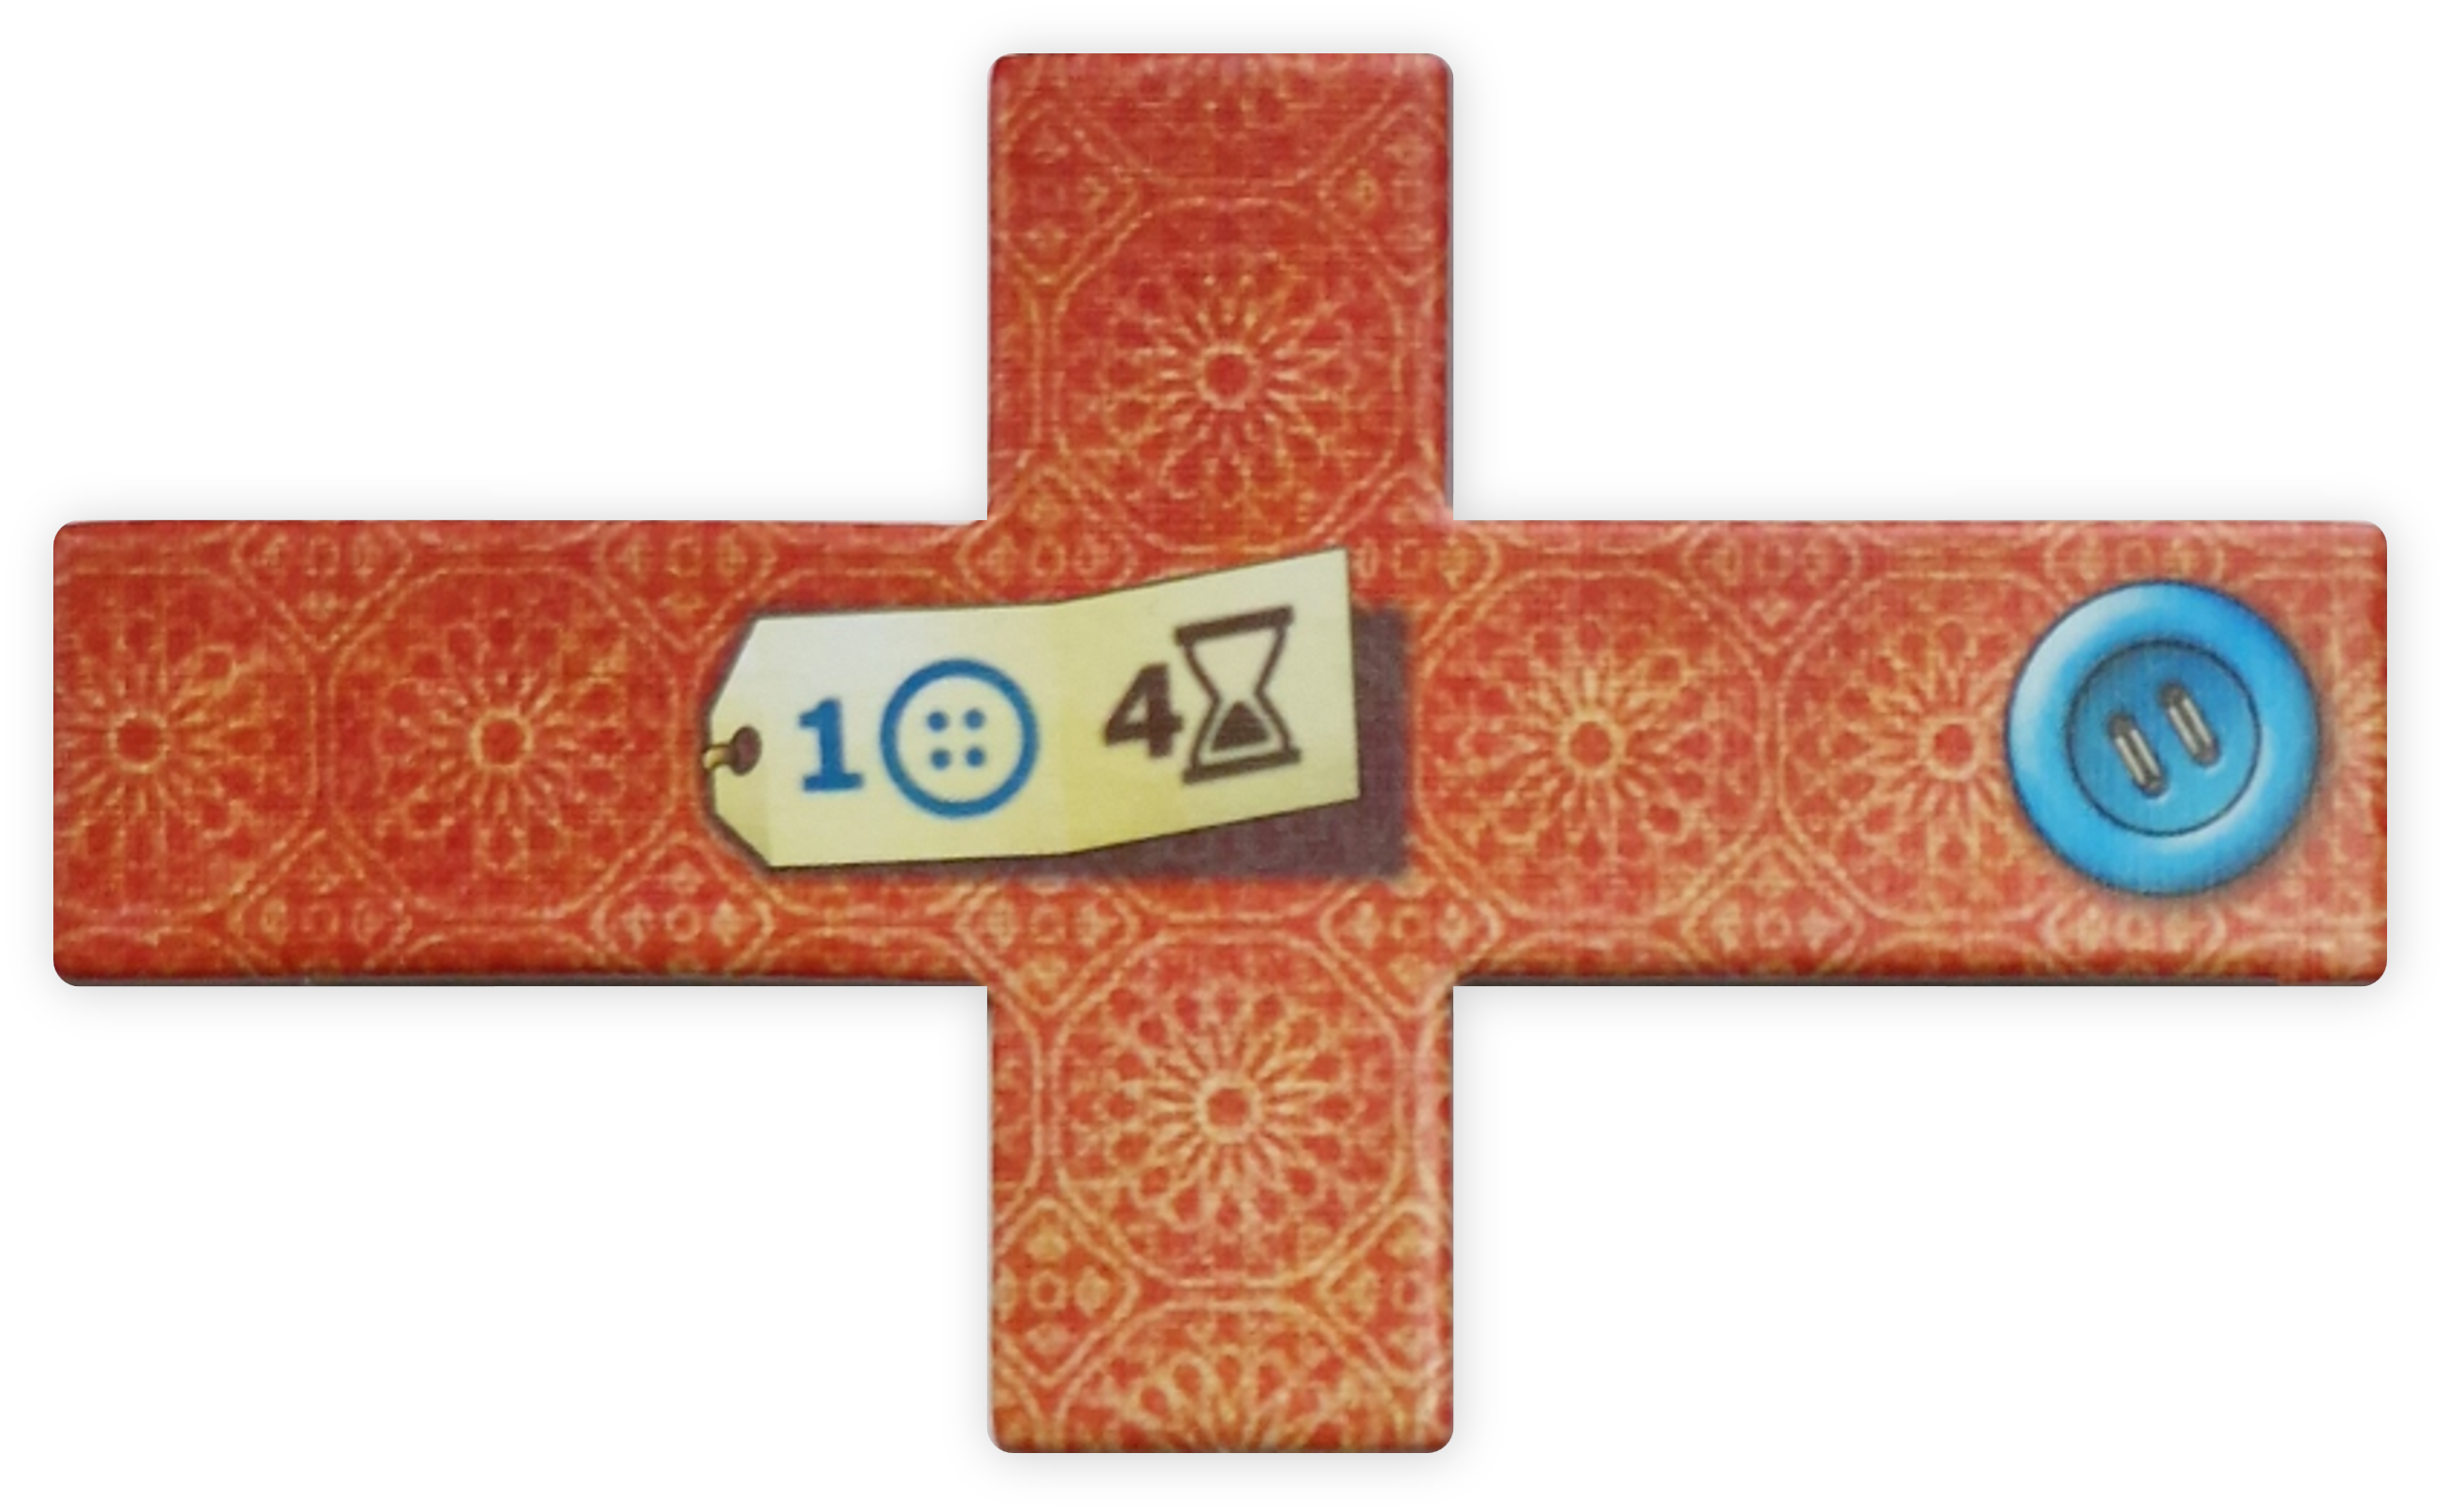
\includegraphics[width=25mm]{res/pictures/assets/20-front.png}};
            \draw[arrow] (take10) -- (take20);

            % walk 2
            \node[right = of take20] (walk2a) {2 laufen};
            \draw[arrow] (take20) -- (walk2a);

            % take 4
            \node[take=4, right = of walk2a] (take04) {\includegraphics[width=15mm]{res/pictures/assets/04-front.png}};
            \draw[arrow] (walk2a) -- (take04);

            % take 3
            \node[take=3, right = of take04] (take03) {\includegraphics[width=15mm]{res/pictures/assets/03-front.png}};
            \draw[arrow] (take04) -- (take03);

            % take 1
            \node[take=1, right = of take03] (take01) {\includegraphics[width=15mm]{res/pictures/assets/01-front.png}};
            \draw[arrow] (take03) -- (take01);

            % take 12
            \node[take=12, right = of take01] (take12) {\includegraphics[width=15mm]{res/pictures/assets/12-front.png}};
            \draw[arrow] (take01) -- (take12);

            % take 30
            \node[take=30, right = of take12] (take30) {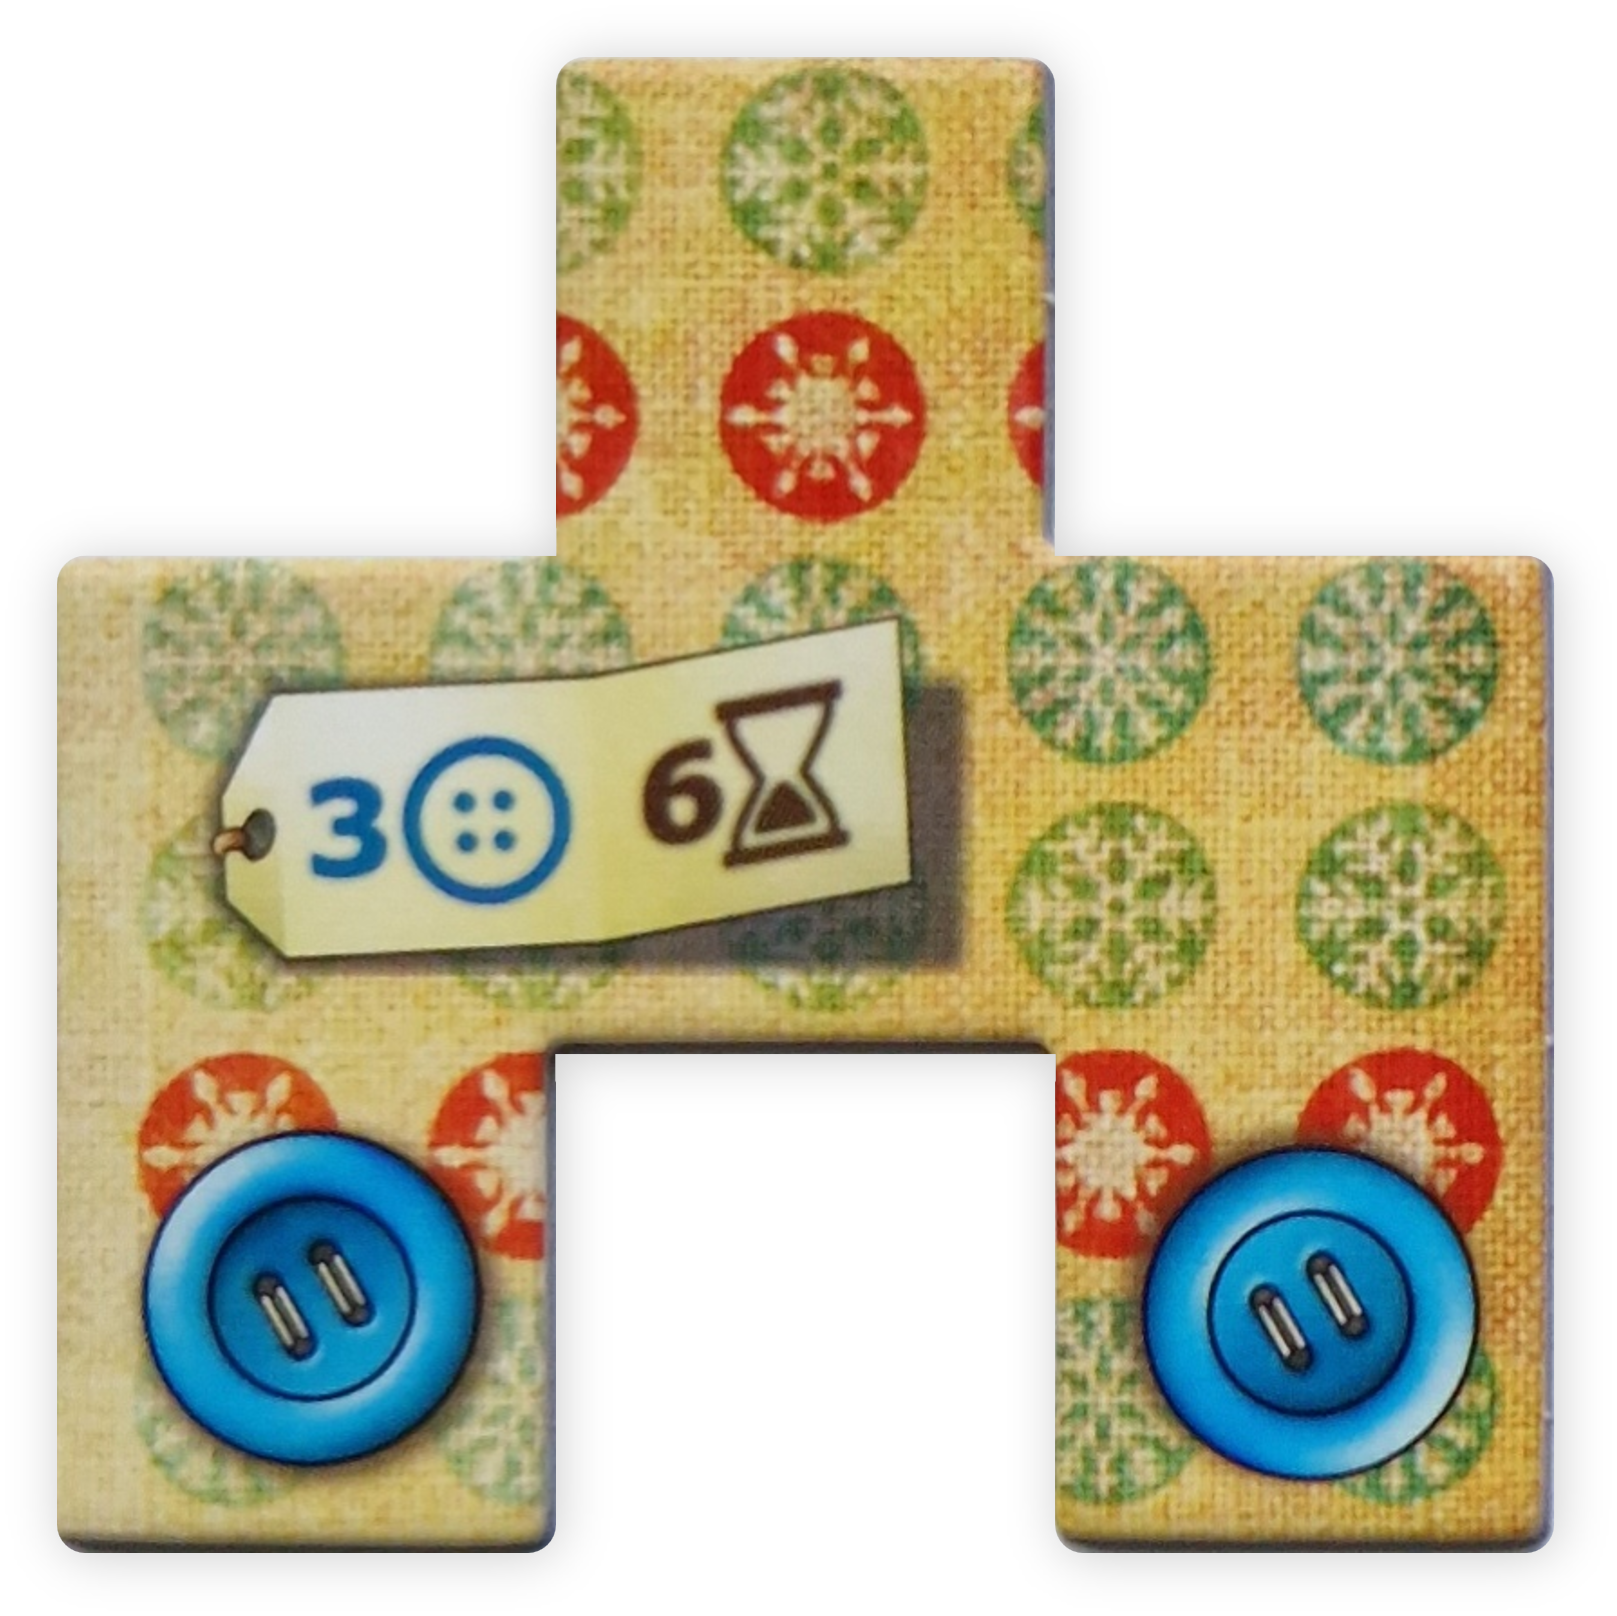
\includegraphics[width=15mm]{res/pictures/assets/30-front.png}};
            \draw[arrow] (take12) -- (take30);

            % take 26
            \node[take=26, below = 5.5cm of take32b -| take30] (take26) {\includegraphics[width=10mm]{res/pictures/assets/26-front.png}};
            \draw[arrow, shorten <=20pt] (take30) -- (take26);

            % parallel
            %     a) walk 2,  take 11, walk 1
            \node[above left = 1cm and 2cm of take26] (walk2p1) {2 laufen};
            \node[take=11, left = of walk2p1] (take11a) {\includegraphics[width=20mm]{res/pictures/assets/11-front.png}};
            \node[left = of take11a] (walk1p1) {1 laufen};
            \draw[arrow] (take26) -|- (walk2p1);
            \draw[arrow] (walk2p1) -- (take11a);
            \draw[arrow] (take11a) -- (walk1p1);
            %     b) take 11, walk 1, walk 2
            \node[take=11, below left = 1cm and 2cm of take26] (take11b) {\includegraphics[width=20mm]{res/pictures/assets/11-front.png}};
            \node[left = of take11b] (walk1p2) {1 laufen};
            \node[left = of walk1p2] (walk2p2) {2 laufen};
            \draw[arrow] (take26) -|- (take11b);
            \draw[arrow] (take11b) -- (walk1p2);
            \draw[arrow] (walk1p2) -- (walk2p2);
            %     c) walk 1, take 11, walk 2 (skip special patch)
            %     d) walk 3, take 11 (skip special patch)

            \coordinate[draw=none, inner sep=0,outer sep=0, left = 2.5cm of take26 -| walk1p1] (dummy) {};
            \coordinate[draw=none, inner sep=0, outer sep=0, left = 0.25cm of dummy] (dummy1) {};
            \coordinate[draw=none, inner sep=0, outer sep=0, right = 0.25cm of dummy] (dummy2) {};
            \draw[very thick, shorten >=2pt] (walk1p1) -|- (dummy);
            \draw[very thick, shorten >=2pt] (walk2p2) -|- (dummy);
            \draw[very thick] (dummy1) -- (dummy2);

            % parallel
            %     b) take 6, take 22, walk 2
            \node[take=6, above left = 0.3cm and 2cm of dummy] (take06b) {\includegraphics[width=15mm]{res/pictures/assets/06-front.png}};
            \node[take=22, left = of take06b] (take22b) {\includegraphics[width=15mm]{res/pictures/assets/22-front.png}};
            \node[left = of take22b] (walk2b) {2 laufen};
            \draw[->, very thick, shorten <=2pt] (dummy) -|-[ratio=.5] (take06b);
            \draw[arrow] (take06b) -- (take22b);
            \draw[arrow] (take22b) -- (walk2b);
            %     a) take 6, walk 2, take 22
            \node[take=6, above = 0.9cm of take06b] (take06a) {\includegraphics[width=15mm]{res/pictures/assets/06-front.png}};
            \node[left = of take06a] (walk2a) {2 laufen};
            \node[take=22, left = of walk2a] (take22a) {\includegraphics[width=15mm]{res/pictures/assets/22-front.png}};
            \draw[->, very thick, shorten <=2pt] (dummy) -|-[ratio=.5] (take06a);
            \draw[arrow] (take06a) -- (walk2a);
            \draw[arrow] (walk2a) -- (take22a);
            %     c) take 22, take 6, walk 2
            \node[take=22, below left = 0.3cm and 2cm of dummy] (take22c) {\includegraphics[width=15mm]{res/pictures/assets/22-front.png}};
            \node[take=6, left = of take22c] (take06c) {\includegraphics[width=15mm]{res/pictures/assets/06-front.png}};
            \node[left = of take06c] (walk2c) {2 laufen};
            \draw[->, very thick, shorten <=2pt] (dummy) -|-[ratio=.5] (take22c);
            \draw[arrow] (take22c) -- (take06c);
            \draw[arrow] (take06c) -- (walk2c);
            %     d) take 22, walk 2, take 6
            \node[take=22, below=1.1cm of take22c] (take22d) {\includegraphics[width=15mm]{res/pictures/assets/22-front.png}};
            \node[left = of take22d] (walk2d) {2 laufen};
            \node[take=6, left = of walk2d] (take06d) {\includegraphics[width=15mm]{res/pictures/assets/06-front.png}};
            \draw[->, very thick, shorten <=2pt] (dummy) -|-[ratio=.5] (take22d);
            \draw[arrow] (take22d) -- (walk2d);
            \draw[arrow] (walk2d) -- (take06d);
            %     e) walk 2, take 6, take 22 (skip special patch)
            %     f) walk 2, take 22, take 6 (skip special patch)

            % take 16
            \node[take=16, left = 4.5cm of dummy -| take06d] (take16) {\includegraphics[width=10mm]{res/pictures/assets/16-front.png}};
            \draw[arrow] (take22a) -|- (take16);
            \draw[arrow] (walk2b) -|- (take16);
            \draw[arrow] (walk2c) -|- (take16);
            \draw[arrow] (take06d) -|- (take16);

            % end
            \node[draw, circle, inner sep=2pt, label=below:Ende] (end) at (start |- take16)  {};
            \draw[arrow] (take16) -- (end);
        \end{tikzpicture}
    \end{adjustbox}
    % \vspace*{-0.5cm}
    \caption{Perfektes Patchwork Spiel}
    \label{fig:max-score-turns}
\end{figure}

Der sich aus dem Optimierungsproblem ergebene perfekte Spielverlauf eines Spielers ist in Grafik \ref{fig:max-score-turns} zu sehen. Zuerst werden Flicken gekauft, die zu ihren vergleichsweißen geringen Kosten viel Knopfeinkommen generieren. Zusammen mit einer Laufaktion kann so im frühem Spielverlauf so viel Knopfeinkommen generiert werden, dass anschließend mehrere Flicken gekauft werden, die das Knopfeinkommen früh deutlich erhöhen. Im weiteren Verlauf des Spiels nimmt die Anzahl der Knopfeinkommen auf den gekauften Flicken immer weiter ab. Das ist wahrscheinlich der Fall, da das noch zu generierende Knopfeinkommen den höheren Preis solcher Flicken im späteren Spielstadium nicht mehr kompensieren kann.

Im spätem Spielverlauf wird nur noch die auf dem Ablageplan gefüllte Fläche vollständig ausgefüllt und alle übrigen \enquote{freien} Aktionen dazu verwendet, durch Laufen den Knopfvorrat weiter zu erhöhen. Als letzte Aktion wird noch der Flicken Nummer 16 genommen, da dieser eine relative große Fläche ausfüllt, ein Knopfeinkommen generiert und nur einen Knopf kostet. Da anschließend direkt das Ziel erreicht wird, sind die großen Zeitkosten von 5 zu vernachlässigen. Am Ende ergibt sich für den Spieler eine maximale Wertung von $\boldsymbol{84}$ Punkten.

\begin{wrapfigure}{r}{0.45\textwidth}
    \vspace*{-0.75cm}
    \centering
    \begin{tikzpicture}
        \node [inner sep=0pt,outer sep=0pt,clip,rounded corners=0.15cm] (image) at (0,0) {\includegraphics[width=0.375\textwidth]{res/pictures/perfect-game.jpg}};
        \drawshadow{image}
    \end{tikzpicture}
    \caption[Ablageplan beim perfekten Spiel]{\unskip}
    Ablageplan beim perfekten Spiel
    \label{fig:max-score-quilt-board}
    \vspace*{-0.75cm}
\end{wrapfigure}

Um zu zeigen, dass es sich bei den $84$ Punkten auch tatsächlich um die maximale Wertung handelt, müssen alle Flicken auch auf dem Ablageplan platzierbar sein. Eine mögliche Kombination hierfür ist in Abbildung \ref{fig:max-score-quilt-board} zu sehen.

Besonders anzumerken ist hierbei, dass der Gegenspieler genau einen der Spezialflicken aufsammeln muss, da der Spieler den fünften Spezialflicken ansonsten auf seinem Ablageplan platzieren müsse und somit keinen Platz mehr für den letzten Flicken hätte. Somit ergibt sich automatisch, dass innerhalb eines Spiels nicht gleichzeitig die maximale Wertung bei einem Spieler und die minimale Wertung bei einem anderen Spieler auftreten kann. Das ist sowieso der Fall, da ein Spieler für die minimale als auch die maximale Wertung den Flicken mit der Nummer 4 kaufen muss.

Weiterhin ist für ein perfektes Spiel eines Spielers neben dem Glück, dass die Flicken am Anfang richtig liegen auch besonders die Kooperation des zweiten Spielers notwendig, sodass alle Aktionen bis zum Ende genauso wie vorgegeben möglich sind. Das ist im Normalfall des kompetitiven Spiels sehr unwahrscheinlich. Jedoch muss aber sichergestellt werden, dass der zweite Spieler genau so agieren kann, dass die oben gezeigten Aktionen des ersten Spielers generell möglich sind. Die Verifikation hierfür wird dem Leser als Übung überlassen. Zuletzt ist noch anzumerken, dass die hier gezeigte Lösung nicht eindeutig ist. Zwei Alternative Spielverläufe, die auch mit einer Wertung von $85$ Punkten enden, sind in Anhang \ref{anhang:section-bilder-spielverlaeufe} gezeigt.

\pagebreak

\section{Auswertung empirischer Daten}

Um die vorangegangenen Betrachtungen genauer einordnen zu können und um gleichzeitig eine realistischere Betrachtung von Patchwork zu erhalten, werden 10 Millionen Spiele von Patchwork aufgenommen und ausgewertet. Dabei treten 2 Computer gegeneinander an, welche für ihren Zug immer eine zufällige Aktion aus allen möglichen Aktionen auswählen (siehe Kapitel \ref{section:erstellung-ansatz-a}). So sollten die 10 Millionen Spiele eine möglichst unverzerrte Datenverteilung enthalten, bei der keine bestimmte Spielkonfiguration bevorzugt wird.

% MEAN: 42.8176
% MEDIAN: 43.0
% MIN: 34 (Count: 4000)
% MAX: 54 (Count: 2000)
% VAR: 8.031931043193113
% STDEV: 2.834066167751401
\begin{figure}[!ht]
    \centering
    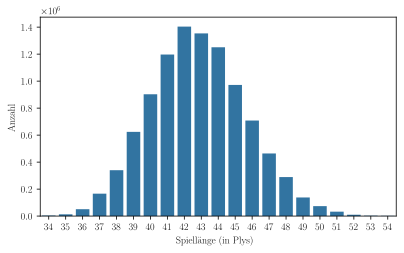
\includegraphics[width=0.7\textwidth]{res/pictures/plots/game_lengths.pdf}
    % \vspace*{-0.5cm}
    \caption{Spiellänge der 10 Millionen Spiele in \hyperref[text:ply]{\emph{Plys}}}
    \label{fig:plot-game-length-10-million}
\end{figure}

Die durchschnittliche Spiellänge, gemessen in \hyperref[text:ply]{\emph{Plys}}, beträgt ${\approx}42{,}8176$. Die kürzesten Spiele der Messung sind nach 34 \hyperref[text:ply]{\emph{Plys}} beendet. Das bedeutet nicht, dass es keine Spiele geben kann, welche kürzer gehen, sondern dass diese in der Messung nicht vorhanden sind. Zu sehen ist das an der maximalen Länge. Hier wurden nur Spiele bis zu einer Länge von 54 \hyperref[text:ply]{\emph{Plys}} erreicht, während wie in »\nameref{subsection:analyse-laenge-des-spiels}« gezeigt auch ein Spielverlauf mit bis zu 63 \hyperref[text:ply]{\emph{Plys}} möglich ist. Die gesamte Verteilung der Spiellänge der empirischen Messung ist in Diagramm \ref{fig:plot-game-length-10-million} zu sehen.

\pagebreak

% MEAN: 83.65933586478253
% MEDIAN: 11.0
% MIN: 1 (Count: 130760000)
% MAX: 1345 (Count: 2000)
% VAR: 22351.213723901034
% STDEV: 149.50322312211543
\begin{wrapfigure}{r}{0.55\textwidth}
    % \vspace*{-0.75cm}
    \centering
    \includegraphics[width=0.549\textwidth]{res/pictures/plots/available_actions.pdf}
    \vspace{-7pt}
    \caption[Verteilung der verfügbare Aktionen]{\unskip}
    Verteilung der verfügbare Aktionen
    \label{fig:plot-available-actions-10-million}
    \vspace{-7pt}
    % \vspace*{-0.85cm}
\end{wrapfigure}

Im Gegensatz zu der normalverteilten Spiellänge, ist die Verteilung der verfügbaren Aktionen, wie in Diagramm \ref{fig:plot-available-actions-10-million} dargestellt ist, stark rechtsschief. Im Diagramm sind dabei keine Aktionen für das Platzieren von Spezialflicken aufgenommen und die Aktionen sind in einer logarithmischen Skala dargestellt. Es existieren deutlich mehr Aktionen mit weniger Möglichkeiten und die durchschnittliche Anzahl an verfügbaren Aktionen liegt bei ${\approx}83{,}66$. Diese rechtsschiefe lässt sich auch leicht erklären: Sobald ein Flicken zu viele Knöpfe kostet oder auf dem Ablageplan keinen Platz findet, fallen auf einen Schlag ungefähr $\sfrac{1}{3}$ der Aktionen weg. Weiterhin fallen immer mehr Platzierungsmöglichkeiten weg, je voller der Ablageplan eines Spielers ist.

\section{Betrachtung der Spiel-Komplexität}

Nachdem nun einige Betrachtungen zu konkreten Wertungen, Aktionen und Spielverläufen von Patchwork gemacht sowie empirische Daten analysiert wurden, wird nachfolgend die spieltheoretische Komplexität untersucht, um eine genauere Vorstellung über die Komplexität von Patchwork im Vergleich zu anderen Spielen zu erhalten.

\subsubsection*{Zustandsraum-Komplexität}

Eine Spieler kann im Spiel aus maximal $3 \cdot 448 + 1 = 1345$ Aktionen wählen und das längste Patchwork-Spiel geht 63 \hyperref[text:ply]{\emph{Plys}}. Somit lässt sich eine einfache obere Schätzung für die Zustandsraum-Komplexität formulieren:

% \vspace*{-1cm}
\begin{align}
    \label{eqn:ssc-patchwork-easy}
    \text{\acsp{SSC}}(Patchwork) & \approx 1345^{63} \approx 1{,}28677884782552 \cdot 10^{197}
\end{align}

Diese Schätzung geht davon aus, dass von der Initialposition immer alle Aktionen möglich sind, das längste Spiel erreicht wird und das der Zustandsraum nach jeder Aktion einzigartig im Vergleich zu allen anderen Zuständen im gesamten Spielbaum ist. Obwohl diese Annahmen sehr unrealistisch sind, werden bei der Komplexitätsbetrachtung oft solche Vereinfachungen zugelassen, die auch nichtexistierende Zustände mitzählen, da dadurch leichter Obergrenzen gefunden werden können. Dadurch, dass jeder Zustand als einzigartig angenommen wird, ist \ref{eqn:ssc-patchwork-easy} auch gleichzeitig eine Obergrenze für die Anzahl der Knoten im Spielbaum, sowie der Anzahl der Blattknoten im Spielbaum / Spielbaumgröße. Somit dürfen alle nachfolgenden Komplexitätsbetrachtungen diese Zahl nicht überschreiten.

Für den Zustandsraum lässt sich auch eine genauere Schätzung verfassen. Ein Spieler besitzt einen Ablageplan mit $81$ Feldern. Diese Felder können immer genau 2 Zustände besitzen, also $2^{81}$. Hinzu kommen $54$ mögliche Positionen, Knopfeinkommen auf dem Ablageplan von $0$ bis $30$ inklusive sowie $184$ Möglichkeiten für die Anzahl der Knöpfe im Knopfvorrat ($\left[-106,\dots,77\right]$). Alle diese Werte wurden zuvor in diesem Kapitel erläutert. Da 2 Spieler existieren, müssen alle diese Werte hoch $2$ genommen werden. Weiterhin gibt es 3 Möglichkeiten für die Vergabe des $7\times 7$ Sonderplättchen (nicht vergeben, Spieler 1 und Spieler 2). Somit ergibt sich als Schätzung für den Zustandsraum von Patchwork:

\begin{align}
    \label{eqn:ssc-patchwork}
    \text{\acsp{SSC}}(Patchwork) & \approx \left(2^{81} \cdot 54 \cdot 31 \cdot 184\right)^{2}\cdot 3 \approx 1{,}66 \cdot 10^{60}
\end{align}

Somit ist es wahrscheinlich, dass es in Patchwork mehr Möglichkeiten für die Platzierung von Flicken, Zeitsteinen und Knöpfen gibt, als Positionen in Schach. Hierfür wurde von S. Chinchalkar eine Obergrenze von $1{,}78\cdot 10^{46}$ berechnet \cite[S. 182]{1996.ChessPositions}. Jedoch ist anzumerken, dass gedrehte und gespiegelte Versionen des Ablageplans als mehrere verschiedene Zustände gelten, obwohl sich dadurch die Komplexität des Spiels nicht vergrößert.

\subsubsection*{Komplexitätstheoretischer Rechenaufwand}

Der komplexitätstheoretische Rechenaufwand für Patchwork ist, wie auch für TicTacToe oder Schach, $\mathcal{O}(1)$, da das Spiel eine feste Brettgröße besitzt und somit nur endlich viele Zustände zulässt. Somit ist es theoretisch möglich eine Tabelle zu konstruieren, bei der zu jedem Zustand angegeben wird, was die beste Aktion ist. Praktisch ist dies aber im Gegensatz zu TicTacToe durch die große Menge an Zuständen nicht umsetzbar.

Oft wird der komplexitätstheoretische Rechenaufwand für Spiele so verallgemeinert, dass die Entwicklung der $\mathcal{O}$-Notation mit beliebig großen Spielfeldern betrachtet wird. Da in dieser Arbeit aber nur Computergegner für das originale Patchwork-Spiel umgesetzt werden, wird dies an dieser Stelle nicht genauer betrachtet.

\subsubsection*{Spielbaumkomplexität}

Mit den empirischen Daten aus dem vorherigem Abschnitt lässt sich eine grobe Schätzung für die Komplexität des Spielbaums in Patchwork erstellen, wobei der durchschnittliche Verzweigungsfaktor mit der durchschnittlichen Spiellänge potenziert wird \cite[S. 160]{1194.SearchAndAiInGames}.

% \vspace*{-1cm}
\begin{align}
    \label{eqn:gtc-patchwork-branch-estimation}
    \text{\acsp{GTC}}(Patchwork) & \approx b^d \approx {83{,}6593}^{42{,}8176} \approx 2{,}08 \cdot 10^{82} \\[2pt]
    \tag*{$\text{mit }           b = \text{durchschnittlicher Verzweigungsfaktor}$}                         \\
    \tag*{$\phantom{\text{mit }} d = \text{durchschnittliche\phantom{r} \rlap{Spiellänge}\phantom{Verzweigungsfaktor}}$}
\end{align}

Die in \ref{eqn:gtc-patchwork-branch-estimation} resultierende Schätzung von $2{,}08 \cdot 10^{82}$ ist dabei jedoch wahrscheinlich zu groß. Der Median der verfügbaren Aktionen beträgt im Gegensatz zum Durchschnitt bei den empirischen Daten nur $11$. Durch einzelne Zustände mit sehr vielen verfügbaren Aktionen wird der Durchschnitt angehoben, obwohl in den meisten Zuständen nur eine oder wenige Aktionen möglich sind.

\subsubsection*{Spielbaumgröße}

Für die Größe des Spielbaums lässt sich nach A. und D. Yong eine recht genaue Schätzung finden. Dazu wird ein Spiel mit $N$ \hyperref[text:ply]{\emph{Plys}} gespielt, wobei die einzelnen Aktionen mittels einer Gleichverteilung ausgewählt werden. In jedem \hyperref[text:ply]{\emph{Ply}} $i$ werden dabei die Anzahl der möglichen Aktionen $c_i(g)$ gespeichert. Aus der Multiplikation all dieser Verzweigungen ergibt sich die Zufallsvariable $X(g)$ als Schätzung für die Größe des Spielbaums. Um nun eine möglichst akkurate Schätzung zu erhalten, wird dieser Prozess in vielen unabhängigen Durchläufen wiederholt und der Mittelwert wie in Formel \ref{eqn:gts-patchwork-avg-estimation} gebildet. Mit $n \to \infty$ nähert sich diese Schätzung immer mehr der tatsächlichen Größe des Spielbaums an. \cite{2019.GameTreeComplexityEstimation}

\begin{equation}
    \label{eqn:gts-patchwork-avg-estimation}
    \begin{aligned}
        X(g)                         & = \prod\nolimits_{j=1}^{N} c_j(g)         \\[15pt]
        \text{\acsp{GTS}}(Patchwork) & \approx \frac{1}{n} \sum_{i=1}^{n} X(g_i) \\[1pt]
                                     & \approx 1{,}68 \cdot 10^{38}
    \end{aligned}
\end{equation}

Als unabhängige Stichproben der Zufallsvariable $X$ können die aufgenommenen 10 Millionen Spiele eingesetzt werden. Somit ergibt sich eine Schätzung der Spielbaumgröße von $1{,}68 \cdot 10^{38}$.

Die Spielbaumkomplexität ist definiert als die Anzahl der Blattknoten im Lösungs-Suchbaum des Startzustandes. Da dieser Lösungs-Suchbaum immer ein Teilbaum des gesamten Spielbaums ist, gilt immer:

\begin{equation}
    \label{eqn:gts-greater-equal-gtc}
    \begin{aligned}
        \forall \mathcal{G} \in \text{Spiele}:\quad \text{\acsp{GTS}}(\mathcal{G}) \geq \text{\acsp{GTC}}(\mathcal{G})
    \end{aligned}
\end{equation}

Somit kann \textendash{} wenn es sich bei \ref{eqn:gts-patchwork-avg-estimation} um eine genügend genaue Schätzung handelt \textendash{} angenommen werden, dass die tatsächliche Spielbaumkomplexität von Patchwork auch unterhalb der $1{,}68 \cdot 10^{38}$ liegt. Diese Schätzung ist höher als die Komplexität von \emph{TicTacToe} mit $255168$ \cite{2024.TicTacToe} oder von \emph{Vier gewinnt} mit $8{,}34 \cdot 10^{28}$ \cite[S. 3]{2019.GameTreeComplexityEstimation} aber geringer als beispielsweise \emph{Othello} mit $6{,}47 \cdot 10^{54}$ \cite[S. 4]{2019.GameTreeComplexityEstimation}. Diese Vergleichswerte für andere Spiele legen nahe, dass Patchwork sich eher der Klasse der komplexeren Spiele zuordnen lässt, sich dabei jedoch eher im unteren Spektrum einordnet. Dieser Umstand wird auch deutlich, wenn man die einfache Schätzung der Spielbaumkomplexität in \ref{eqn:gtc-patchwork-branch-estimation} mit einer äquivalenten Schätzung für Schach mit $10^{120}$ von Shannon vergleicht \cite[S. 4]{1950.ChessShannon}. Patchwork ist zwar insgesamt weniger komplex, jedoch immer noch viel zu komplex als dass das gesamte Spielgeschehen vorhergesehen werden kann oder Brute-Force-Algorithmen alles vorausberechnen können. Das wird vor allem dann ersichtlich, wenn man die Spielbaumkomplexität mit der großen Zustandsraum-Komplexität kombiniert. Patchwork lässt sich zusammen mit anderen Spielen in einem 2-dimensionalen-Koordinatensystem mit den Achsen \emph{$\log_{10} \log_{10} \text{Zustandsraum-Komplexität}$} und \emph{$\log_{10} \log_{10} \text{Spielbaumkomplexität}$} plotten (Abbildung \ref{fig:game-complexity-coordinate-system})\footnote{Die Komplexitätswerte der anderen Spiele sind dabei von Quelle \cite[S. 300]{2002.GamesSolved} übernommen}. Dabei reiht sich Patchwork zusammen mit Schach oder Hex ein.

\begin{figure}[!ht]
    \centering
    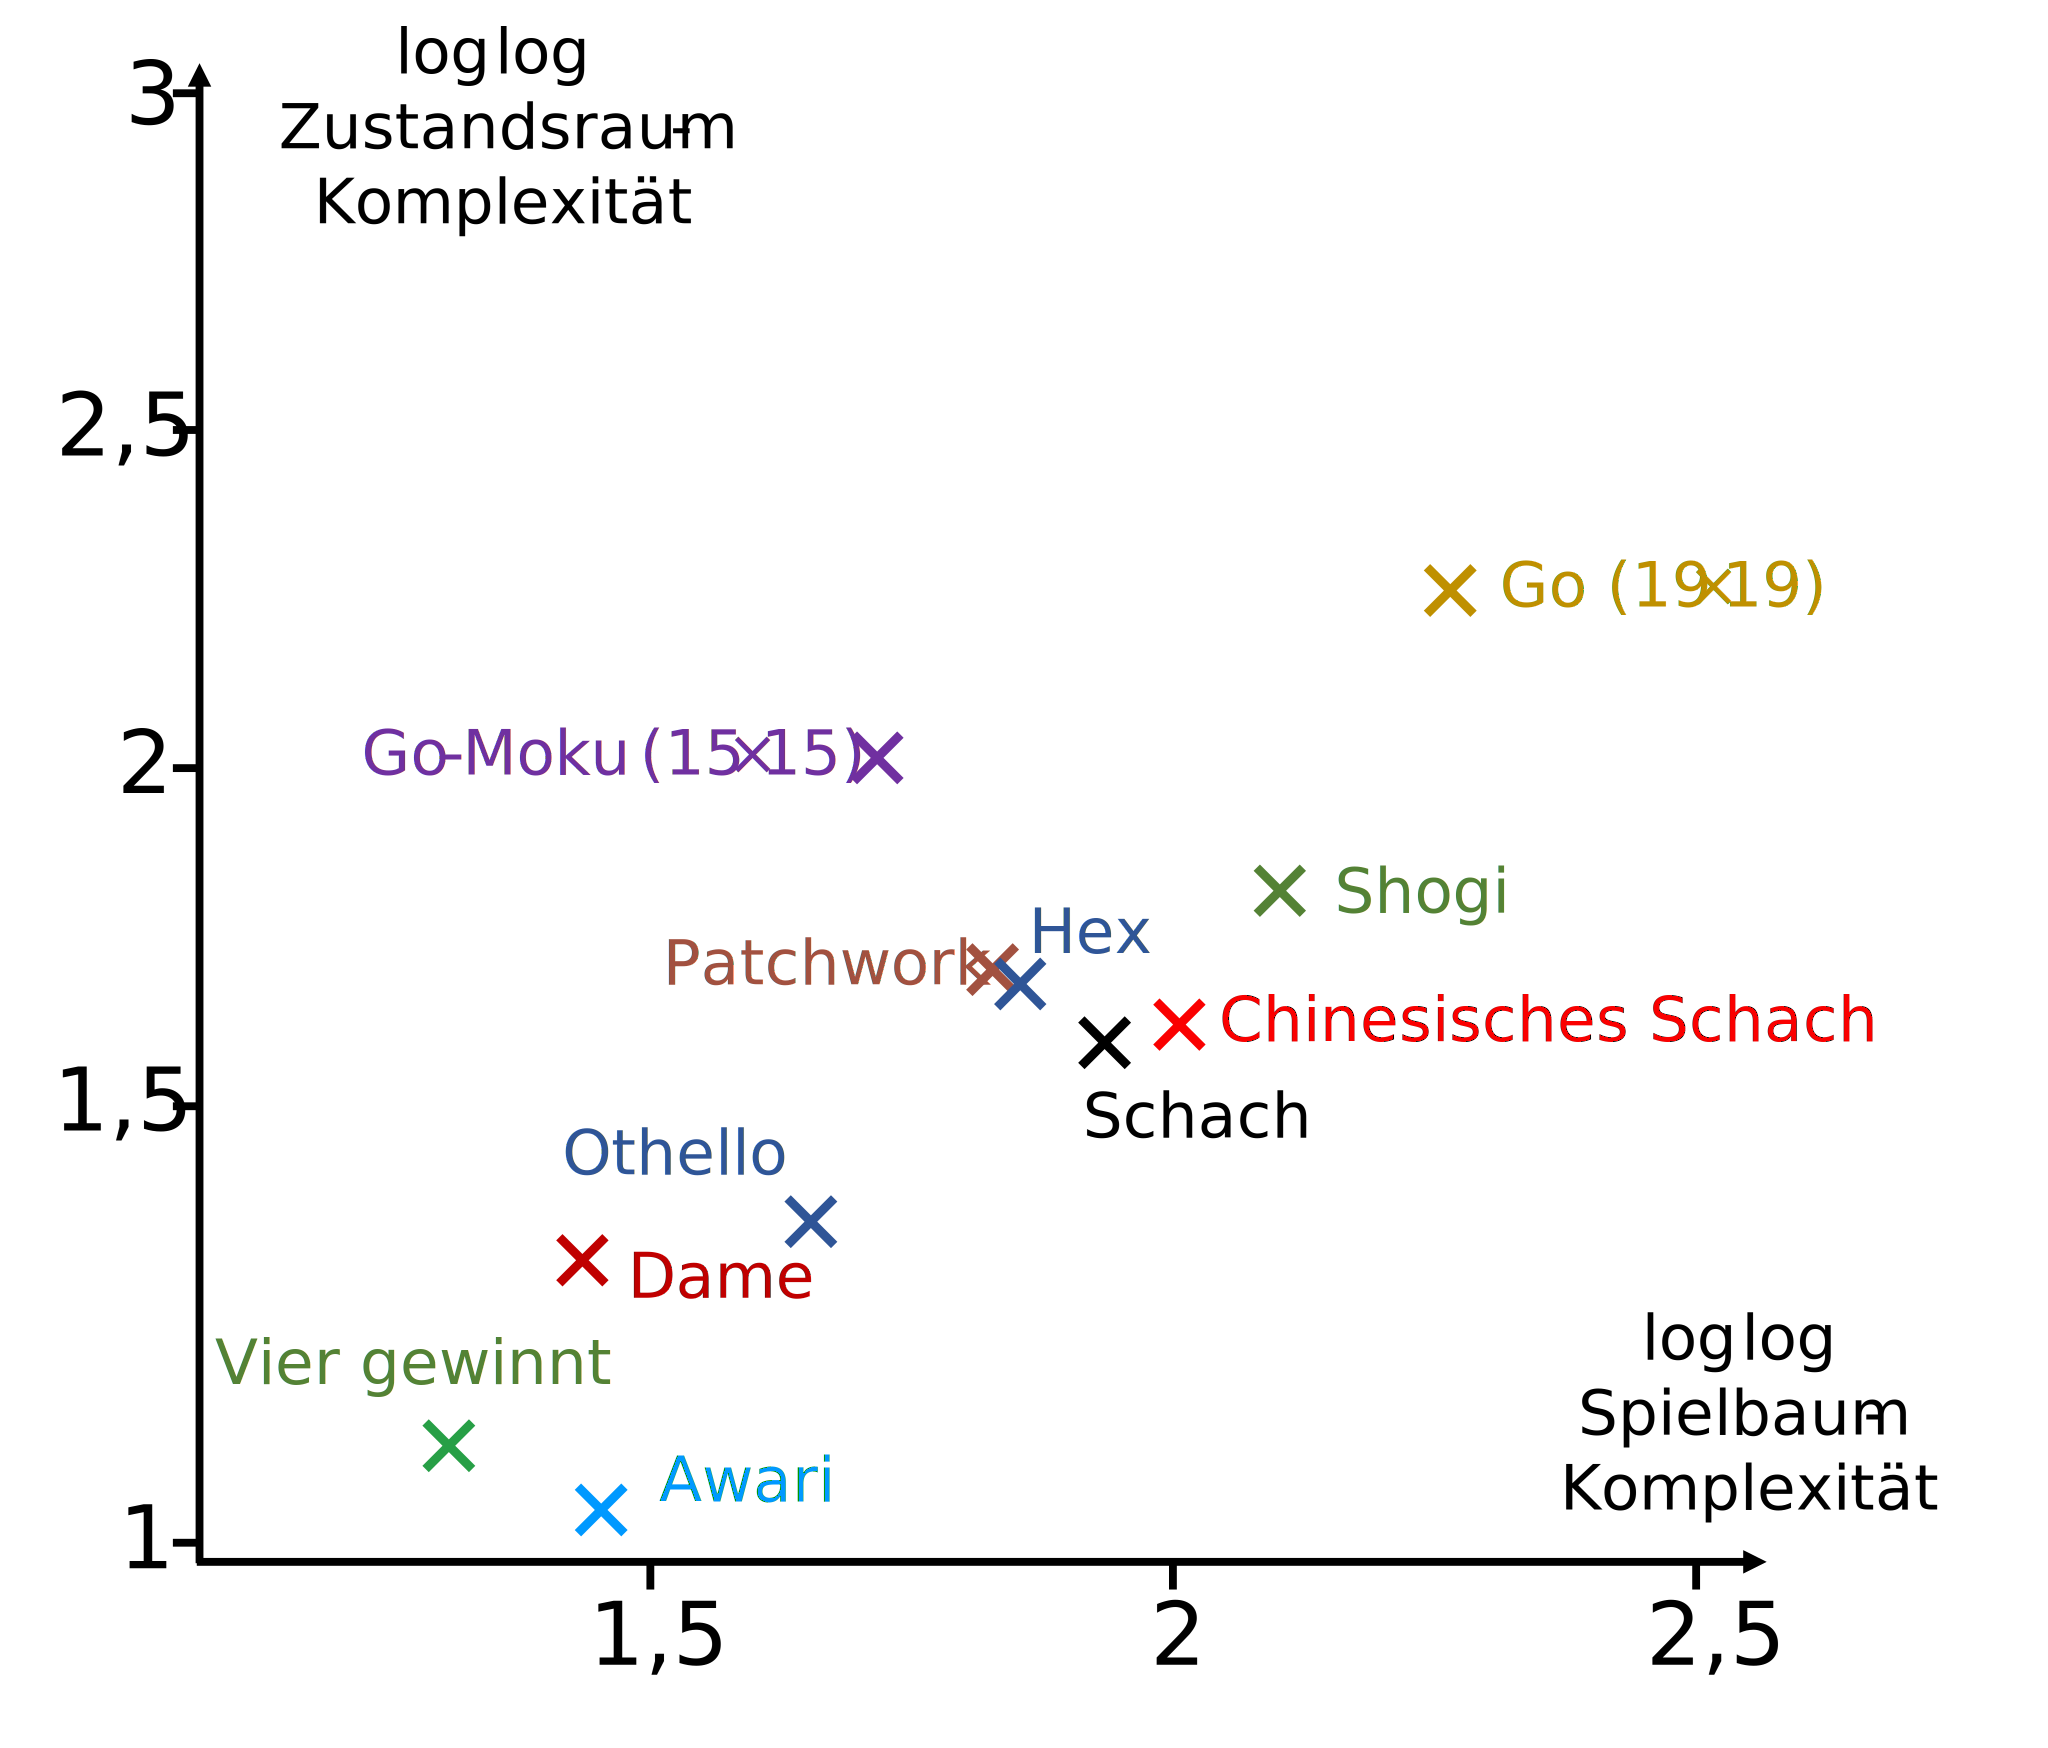
\includegraphics[width=0.85\textwidth]{res/pictures/game-complexity-coordinate-system.pdf}
    \caption{Patchwork in der doppelten Dichotomie des Spielraums}
    \label{fig:game-complexity-coordinate-system}
\end{figure}

\vfill
\vspace*{100cm}

% sum k=1 to n of P(n, k) = n! / (n-k)! = 36! / (36-k)! = 36! / (36-36)! = 36! / 0! = 36!

% import math
% result = 0
% for k in range(1, n+1):
%     result += math.factorial(36) // math.factorial(36 - k)
% print(result)

% P(3) = 15
% P(2) = 6
% P(1) = 3

% 1*6+3*2+3*1=15

% (1,2,3) * 3!
% (1,2) * 2!
% (1,3) * 2!
% (2,3) * 2!
% (1) * 1!
% (2) * 1!
% (3) * 1!
% ()  * 0!

\chapter[Modellierung als Computerprogramm]{Modellierung von Patchwork als Computerprogramm}
\label{chapter:modellierung-von-patchwork-als-computerprogramm}

Ein wesentlicher Schritt in der Entwicklung von Computerspielengines besteht in der Modellierung und Umsetzung des Spiels als Computerprogramm. Da Engines in der Regel darauf basieren mehrere zehntausende von Aktionen vorrausschauen \cite{2018.AlphaZero}, muss die zugrundeliegende Implementierung so effizient wie möglich sein. Eine erste prototypische Implementierung von Patchwork in Python führte zu Zuggenerierungszeiten von ca. $100\acs{ms}$, was in 10 Sekunden aber gerade mal die Analyse von 100 möglichen Zügen bedeutet. Aus diesem Grund wird Patchwork mit der Programmiersprache \emph{Rust} \cite{2014.Rust} umgesetzt. Rust hat Performance als ein Hauptziel und zeichnet sich durch eine schnelle und speichereffiziente Ausführung aus \cite{2024.Rust}. Zusammen mit weiteren Effizienzoptimierungen führt dies zu Ausführungszeiten im Mirkosekundenbereich (Tabelle \ref{tabelle:patchwork-methods}).

\lstinputlisting[
    label={code:patchwork-state},
    caption={Patchwork-Zustand},
    captionpos=b,
    language=Rust,
    firstline=0,
]{res/code/patchwork-state.rs}

Der gesamte Zustand von Patchwork wird zu jeder Zeit durch die in Codeausschnitt \ref{code:patchwork-state} dargestellte Struktur \code{Patchwork} repräsentiert. Alle noch verfügbaren Flicken werden in \code{patches} in der Reihenfolge gespeichert, wie sie vor der Spielfigur liegen. Der \code{turn\_type} zeigt an, ob es sich bei den derzeit verfügbaren Aktionen um eine normale Aktion handelt oder ob ein Spezialflicken gelegt werden muss. Der derzeitige Spieler, der Inhaber des $7\times 7$ Sonderplättchens und der Spieler, welcher als erstes das Ziel erreicht hat, werden im Bitfeld \code{status\_flags} festgehalten, sofern vorhanden. Letzteres ist relevant, um bei einem beendeten Spiel mit gleicher Punktzahl den Gewinner identifizieren zu können.

Der Zeitplan wird mittels der \code{TimeBoard}-Struktur modelliert. Diese hält intern nur ein einfache \ac{u8}-Array der Länge 54. Bei jedem Eintrag des Arrays handelt es sich wiederrum um ein Bitfeld. Dieses kann signalisieren, ob sich Spieler 1 und 2, ein Knopfeinkommen oder ein Spezialflicken auf ihrem Feld befindet. Knopfeinkommen und Spezialflicken befinden sich im originalen Spiel zwischen 2 Feldern. Im Array werden sie einfach in dem Feld nach ihrer Originalposition gespeichert. Sobald solch ein Feld von einem Spieler erreich wird, tritt der Effekt ein, was zu gleichem Verhalten wie im Brettspiel führt.

Zuletzt existiert für jeden Spieler noch ein Zustand in der Patchwork-Struktur. Der Zustand jeden Spielers setzt sich dabei aus 3 Komponenten zusammen. Zuerst wird hier auch die Position des Spielers gespeichert, um Zugriff in konstanter Zeit zu ermöglichen. Weiterhin wird der derzeitig verfügbare Knopfvorrat des Spielers gespeichert. Zuletzt wird noch auf eine weitere Struktur, das \code{QuiltBoard}, verwiesen.

\section{Aufbau des Ablageplans}

\lstinputlisting[
    label={code:quilt-board-definition},
    caption={Definition der QuiltBoard-Struktur},
    captionpos=b,
    language=Rust,
    firstline=0,
]{res/code/quilt-board-definition.rs}
\vspace*{-0.3cm}

Die in Codeausschnitt \ref{code:quilt-board-definition} definierte Struktur \code{QuiltBoard} modelliert den Ablageplan eines Spielers. Dabei existieren nur 2 Attribute. Zuerst wird das Knopfeinkommen mit \code{button\_income} gespeichert, was durch die auf dem Ablageplan liegenden Flicken beim Passieren einer Knopf-Wertung generiert wird. Das zweite Attribut \code{tiles} dient dazu, den Status der einzelnen Felder auf dem Ablageplan zu speichern. Der Ablageplan besteht aus 81 Feldern, die in 9 Zeilen und 9 Spalten angeordnet sind, und für die jeweils gespeichert werden muss, ob das Feld belegt ist oder nicht. Da alle Abfragen bezüglich Status der Felder so schnell wie möglich sein sollen, kommt hier anstatt eines üblichen 2-dimensionalen Arrays eine \ac{u128} zum Einsatz. Da nur zwei Zustände existieren, kann für jedes Feld ein Bit verwendet werden. Weiterhin werden alle Felder des Ablageplans zeilenweise wie in Abbildung \ref{fig:quilt-board-storage} in einer Ganzzahl nacheinander abgelegt.

\vspace*{-5cm}
\pagebreak

\begin{figure}[!ht]
    \centering
    \rlap{{\color{white}\acf{LSB} \acf{MSB}}} \vspace*{-\baselineskip}
    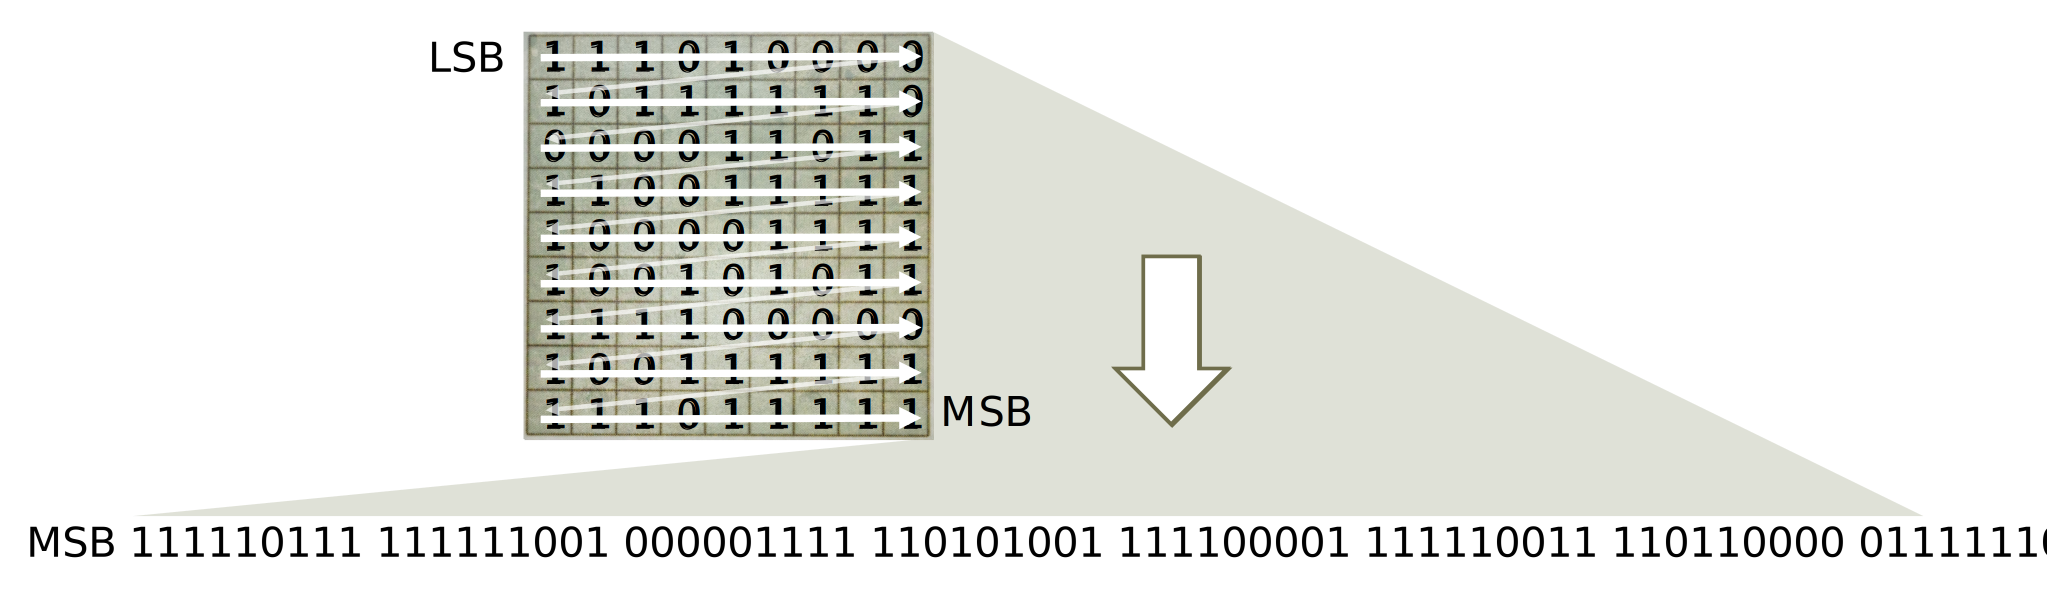
\includegraphics[width=\textwidth]{res/pictures/quilt-board-storage.pdf}
    \caption{Zeilenweise Anordnung der Felder des Ablageplans}
    \label{fig:quilt-board-storage}
\end{figure}

Da der Ablageplan 81 Felder umfasst, muss $2^7=128$ Bit als Ganzzahldatentyp verwendet werden. Dieser wird von Rust nativ unterstützt und für 64 Bit Rechner in mehrere Operationen kompiliert. Die oberen Bits der Zahl sind dabei immer auf 0 gesetzt. Durch die effiziente Speicherung des Ablageplans in einem \ac{u128}, können Abfragen bezüglich Befüllung oder Überlagerung von Feldern in konstanter Zeit durch Bitmasken und Bitoperationen durchgeführt werden. Als Beispiel lässt sich hier die Methode zum Überprüfen der notwendigen Bedingung zur Erhaltung des $7\times 7$ Sonderplättchen anführen (Anhang \ref{code:quilt-board-special-tile-condition}).

Besonders anzumerken ist, dass die Flicken und ihre Transformationen, wie sie auf dem Ablageplan liegen, nicht gespeichert werden. Da einige Computergegner wie beispielsweise der \ac{MCTS}-Spieler den Spielstand sehr oft kopieren müssen und die genaue Position der Flicken für die Generierung und Ausführung von Aktionen nicht benötigt wird, würde diese Extrainformation nur zu unnötig erhöhtem Speicherverbrauch führen.

\section{Modellierung der Aktionen}

Wie in Codeauschnitt \ref{code:action} zu sehen, sind die Spielzüge von Patchwork für das Computerspiel als \code{enum} umgesetzt, das folgende Aktionen definiert:
\begin{itemize}
    \item Die Aktion \code{Walking} beschreibt die Laufaktion eines Spielers startend vom Feld \code{starting\_index}.
    \item Die Aktion \code{PatchPlacement} beschriebt das Platzieren des Flickens mit der einzigartigen \ac{ID} \code{patch\_id}. Der Flicken muss einer der drei durch den aktuellen Spieler auswählbaren Flicken sein und wird unter diesen mit dem \code{patch\_index} identifiziert. In \code{patch\_transformation\_index} wird die jegliche Transformation des Flickens gespeichert, d.h. wie der Flicken gespiegelt, rotiert und wo er auf dem Spielfeld abgelegt wurde. Ob im vorigen Zug Spieler 1 an der Reihe war, wird im Attribut \code{previous\_player\_was\_1} gespeichert.
    \item Bei der Aktion \code{SpecialPatchPlacement} wird ein Spezialflicken auf das Spielfeld auf die Position des \code{quilt\_board\_index} gelegt.
    \item Die Aktion \code{Phantom} beschriebt einen Spielzug, indem der Spieler nichts tut. Diese Aktion kann im normalen Spielverlauf nicht vorkommen, wird allerdings für einige \ac{KI}-Gegner benötigt. Dies ist der Fall, in dem ein erzwungener Spielerwechsel stattfinden soll, also für die Situation in der eigentlich Spieler 1 an der Reihe wäre, aber Spieler 2 jetzt ziehen soll.
    \item Die Aktion \code{Null} kennzeichnet einen illegalen Zug.
\end{itemize}

\lstinputlisting[
    label={code:action},
    caption={Definition des Tagged-Union \code{Action}},
    captionpos=b,
    language=Rust,
    firstline=0,
]{res/code/action.rs}

Um diese Aktionen kompakter zu speichern und die effizientere Verarbeitung mit einem Computer zu ermöglichen, existiert die Struktur \code{ActionId}, welche aus einer Variablen mit dem Typ \ac{u32} besteht. In dieser einen Zahl der folgenden Ganzzahl-Intervalle werden alle Aktionen als Surrogat eindeutig codiert und wie folgt gespeichert:
\begin{itemize}
    \item Eine \ac{ID} aus $[0, 52]$ beschreibt die Laufaktion, wobei die Zahl das Startfeld repräsentiert.
    \item Eine \ac{ID} aus $[53, 133]$ beschreibt den Ablageort eines Spezialflickens, die Zahl repräsentiert die Position mittels Spielfeldindex.
    \item Eine \ac{ID} aus $[134, 88.837]$ beschreibt eine Flickenplatzierung, wobei dieselben Information wie bei dem vorher beschriebenen \code{Action}-Enum codiert gespeichert werden.
    \item Die Zahl 88.838 repräsentiert die Phantom-Aktion und folgende Zahl 88.839 die Null-Aktion.
\end{itemize}
Während die \code{ActionId} sehr gut für die Spielimplementierung geeignet ist, eignet sich diese aber nicht für die Ausgabe eines neuronalen Netzes. Ein Computernetzwerk sollte immer entscheiden, welche der ersten drei Flicken platziert werden soll. Die \code{ActionId} besitzt für diese Aufgabe durch ihren großen Zahlenbereich von ca. 90.000 Werten zu viel Overhead. So werden unter anderem für die Entscheidung unnötige Informationen wie der genaue Transformationsindex in der \code{ActionId} gespeichert. Aus diesem Grund existiert noch die \code{NaturalActionId}, welche als \ac{u64} Zahl kodiert ist. Hierbei wird mit der \ac{ID} 0 die Laufaktion codiert. Von 1 bis 81 werden die Platzierung für Spezialflicken mit Zeilen- und Spalteninformation codiert. Im Gegensatz zur \code{ActionId} werden danach alle weiteren Aktionen, die Flickenplatzierungen, im Bereich von 82 bis 2.025 codiert, indem nur gespeichert wird, welcher der ersten drei Flicken gewählt wurde und in welcher Reihe, Spalte, Rotation und Orientierung der Flicken platziert wurde. Die letzten beiden Zahlen codieren wieder die Phantom-Aktion (2.026) und die Null-Aktion (2.027).

Die oberen Bits der \code {NaturalActionId} werden zur Speicherung von Informationen verwendet, welche für die Umwandlung zurück in eine \code{ActionId} benötigt werden. Für die Ausgabe eines neuronalen Netzes sind diese Bits nicht relevant.

\section{Flicken}

Die Speicherung der Flicken im Computerprogramm ist aufwendiger. Der \code{PatchManager} übernimmt die Verwaltung der Flicken und stellt eine zentrale Zugriffmöglichkeit auf alle Flicken in der gesamten Applikation dar. So kann über den PatchManager beispielsweise die zufällige initiale Flickenreihenfolge zum Spielstart generiert werden oder ein Index auf dem Zeitplan zu einem konkretem Spezialflicken bidirektional zugeordnet werden. Um sicherzustellen, dass es immer nur genau eine Instanz des PatchManagers existiert, wird dabei das Entwurfsmuster Singleton implementiert \cite[S. 127]{2000.Gamma}.

Ein Flicken wird im Code als Patch bezeichnet und besteht aus einem eindeutigen Identifizierter, Knopf- und Zeitkosten sowie Knopfeinkommen. Der PatchManager speichert alle Patches in einem Array und erlaubt den Zugriff auf diese. Neben diesen einfachen Patch-Strukturen erlaubt der PatchManager aber auch noch Zugriff auf die sogenannten PatchTransformationen für jeden Flicken. Da der Ablageplan als eine einzige 81-bit lange Zahl abgespeichert ist, sind das Erkennen von Überlappungen und das Legen von Flicken in konstanter Zeit durch Und- sowie Oder-Bitoperationen möglich. Dafür muss nur für jeden Flicken und jede Platzierungsmöglichkeit die passende Zahl nach der gleichen Anordnung wie beim Ablageplan generiert werden. Die Erzeugung solch einer Zahl zur Laufzeit dauert jedoch im Vergleich zu anderen Operationen viel zu lange. Da die Anzahl der Flicken und ihrer Platzierungsmöglichkeiten aber begrenzt sind, kann für jeden Flicken bereits jede Mögliche Platzierungslage als \ac{u128} vorausberechnet werden. Der PatchManager hält dann alle diese vorausberechneten Transformationen in einer Liste. Eine Transformation besteht dabei neben der vorausberechneten Zahl noch aus dem genauen Platzierungsort mit Zeile, Spalte und der Transformation (Drehung sowie Spiegelung). Zuletzt speichert der PatchManager noch die genauen Felder der Flicken als $m\times n$-Matrix zu Darstellungszwecken. Alle drei Datentypen sind auch in Codeauschnitt \ref{code:patch} dargestellt.

\lstinputlisting[
    label={code:patch},
    caption={\code{PatchManager}, \code{Patch} und \code{PatchTransformation}},
    captionpos=b,
    language=Rust,
    escapeinside={<*}{*>},
    firstline=0,
]{res/code/patch.rs}
\begin{tikzpicture}[
        remember picture,
        overlay
    ]
    \draw[->] (pic cs:patch-line-2-first) ++(-0.25cm,.5ex) -| ++(-1cm,-2.6cm);
    \draw[->] (pic cs:patch-line-4-end) ++(0,-1ex) -| ++(0,-1.1cm);
\end{tikzpicture}
\vspace*{-1cm}

Für die Generierung aller Flicken werden funktionsähnliche Prozedurale Makros von Rust verwendet. Diese erlauben zu Kompilierungszeit das Entgegennehmen von Tokens und generieren aus diesen validen Rust Code \cite[S. 673]{2023.RustBook}. Um die Flicken zu erzeugen, wird das Makro \code{generate\_patches!} verwendet, welches eine eigengeschriebene Funktion ist, von Rust zur Kompilierungszeit aufgerufen wird und alle Flicken, Transformationen und Felder erzeugt. So können alle Flicken ergonomisch wie in \code{code:patch-macro} definiert werden. Das Makro berechnet dann alle Werte und fügt sie in die passenden Attribute im PatchManager ein, sodass am Ende ein vollständig befüllter PatchManager mit allen Flicken zurückgegeben wird. So kann während der Laufzeit mittels Indices auf die statisch in die Applikation eingebetteten Werte zugegriffen werden.

\lstinputlisting[
    label={code:patch-macro},
    caption={Definition eines Flicken mittels Makro},
    captionpos=b,
    language=Rust,
    escapeinside={<*}{*>},
    firstline=0,
]{res/code/patch-macro.rs}

\section{Zugmöglichkeiten}

Die Methode \code{get\_valid\_actions} existiert, um die verschiedenen verfügbaren Aktionen zu generieren. In dieser Methode wird zuerst überprüft, ob sich der Spielzustand in einem Phantomzustand befindet. Ist dies der Fall, wird die Phantom-Aktion zurückgegeben. Weiterhin wird überprüft, ob sich der Spielzustand in \emph{SpecialPatchPlacement} befindet. In diesem Zustand wurde zuletzt ein Spezialflicken eingesammelt und muss nun gelegt werden. Deshalb wird beim Ablageplan des derzeitigen Spielers passende Methode aufgerufen, welche für jedes freie Feld auf dem Ablageplan eine Aktion zurückgibt. In allen anderen Fällen handelt es sich um einen normalen Spielzug, bei dem eine Liste an Aktionen erstellt wird. In dieser Liste befindet sich immer die Lauf-Aktion. Weiterhin wird für jeden der 3 verfügbaren Flicken die Methode \code{get\_valid\_actions\_for\_patch} auf dem Ablageplan des derzeitigen Spielers aufgerufen. Die in \ref{code:quilt-board-valid-actions} dargestellte Methode kann aufgrund der Speicherart des Ablageplans und der transformierten Flicken einfache Bitoperationen durchführen um alle validen Aktionen eines Flicken zu generieren.

\lstinputlisting[
    label={code:quilt-board-valid-actions},
    caption={[Aktionsgenerierung auf dem Ablageplan]Generierung der möglichen Aktionen auf dem Ablageplan},
    captionpos=b,
    language=Rust,
    firstline=0,
]{res/code/quilt-board-get-valid-actions-for-patch.rs}

Um die Implementierung dennoch so schnell wie möglich zu gestalten, werden vor dem Methodenaufruf im Ablageplan noch zwei einfache Bedingungen überprüft:

\begin{itemize}
    \item Sind die Knopfkosten des Flickens höher als der Knopfvorrat des derzeitigen Spielers?
    \item Sind auf dem Ablageplan des derzeitigen Spielers weniger Felder frei, als der Flicken groß ist?
\end{itemize}

Beide diese Bedingungen können durch schnellen Zugriff auf bereits vorhandene Attribute implementiert werden. Ist eine dieser Bedingungen falsch, so müssen für den jeweiligen Flicken keine validen Aktionen auf dem Ablageplan generiert werden, \dash es wird Zeit eingespart.

\section{Spielverlauf}

Nachdem nun die grundlegenden Bausteine der Implementierung erklärt sind, kann sich dem Spielverlauf zugewendet werden. Der grundlegende Aufbau eines Spielverlaufes ist in Pseudocode \ref{algo:spielverlauf} dargestellt.

\refstepcounter{lstlisting}
\addcontentsline{lol}{lstlisting}{\protect\numberline{\thelstlisting}Pseudocode für einen Spielverlauf}

\begin{algorithm}
    \caption{Pseudocode für einen Spielverlauf}
    \label{algo:spielverlauf}
    \begin{algorithmic}[1]
        \Function{game\_loop}{}
        \State $state \gets Patchwork::\Call{get\_initial\_state}$
        \While{not $state.\Call{is\_terminated}$}
        \If{current player is 1}
        \State $action \gets player1.\Call{get\_action}$
        \Else
        \State $action \gets player2.\Call{get\_action}$
        \EndIf
        \State $state \gets state.\Call{do\_action}{action}$
        \EndWhile
        \State $result \gets state.\Call{get\_termination\_result}$
        \EndFunction
    \end{algorithmic}
\end{algorithm}

Jedes Spiel beginnt zuerst damit, dass der Startzustand geladen wird (Anhang \ref{code:get-initial-state}). Dabei werden wie vorgegeben jedem Spieler 5 Knöpfe und ein leerer Ablageplan zugewiesen sowie ein Zeitplan im initialen Zustand erstellt. Weiterhin gibt der PatchManager eine zufällig gemischte Liste an allen Flicken zurück. Dann wiederholen sich die Spielzüge bis zum Ende des Spiels. In jedem Spielzug muss der derzeitige Spieler, bei dem es sich sowohl um einen menschlichen Spieler als auch eine Computerengine handeln kann, eine Aktion auswählen. Die Auswahl einer Aktion wird im \hyperref[chapter:erstellung-der-computerspielengines]{5. Kapitel} genauer beschrieben. Anschließend wird die Action mittels der Methode \code{do\_action} ausgeführt. Die Methode führt dabei einfach die in den Spielregeln beschriebenen Schritte aus (Anhang \ref{code:do-action}). So wird zum Beispiel bei dem Legen eines Flickens der Ablageplan gefüllt, die Knopfkosten vom Knopfvorrat des Spielers abgezogen und der Zeitstein um die Zeitkosten des Flickens vorbewegt. Zuletzt wird noch überprüft, ob eine Knopf-Wertung oder ein Spezialflicken passiert wurde und welcher Spieler als nächstes dran ist. Um ein Flicken auf dem Ablageplan abzulegen, wird einfach die passende Transformation aus dem PatchManager geladen und mittels einer Oder-Bitoperation auf den bestehenden Ablageplan gelegt.

Ein Spiel ist im Endzustand angelangt, wenn $Player\, 1\, Position \ge \max\, Zeitplan\, Position$ $\wedge\, Player\, 2\, Position \ge\, \max\, Zeitplan\, Position$, also beide Spieler im Ziel sind. Nach dem Spiel lässt sich das Ergebnis über \code{get\_termination\_result} Abfragen. Diese Methode gibt neben dem Gewinner noch die Wertungen der beiden Spieler am Spielende zurück (Anhang \ref{code:get-termination-result}). Die Wertung des Gewinners ist immer größer gleich der Wertung des Verlierers, kann aber nach den Spielregeln auch gleich sein.

In Tabelle \ref{tabelle:patchwork-methods} sind abschließend einige der wichtigsten Methoden für die Umsetzung von Patchwork als Computerspiel aufgelistet zusammen mit ihrer Komplexität im $\mathcal{O}$-Kalkül und der durchschnittlich benötigten Zeit.

Die benötigte Zeit der Methoden wurde dabei mittels Benchmarks ermittelt. Für die Benchmarks wird \enquote{Criterion.rs} verwendet. Criterion ist eine extra für Mikro-Benchmarking zwecke entwickelte Bibliothek, welche versucht unter anderem mittels statistischer Methoden möglichst akkurate Ergebnisse zu erzeugen \cite{2018.Criterion}. Dazu werden alle Benchmarks vor der Zeitmessung zuerst mehrmals hintereinander in einer Warmup-Phase ausgeführt und dann so lange wiederholt, bis ein stabiles Ergebnis zustande kommt \cite{2018.CriterionAnalysis}. Aus den aufgenommenen Ausführungen der Benchmarks wird dann neben einem Punktschätzer, der Mittelwert der Ausführungen, auch ein Konfidenzintervall gebildet, in welchem das tatsächliche Ergebnis mit einer 95\%-igen Wahrscheinlichkeit liegt \cite{2019.CriterionOutput}. Um bei den Zeitmessungen dennoch so verlässliche Werte wie möglich zu erhalten, wurden diese bereits sehr stabilen Benchmarks zu verschiedenen Zeitpunkten insgesamt 10-mal wiederholt. In Tabelle \ref{tabelle:patchwork-methods} ist der Median der Punktschätzer all dieser Durchläufe abgebildet. Der Quellcode für die Performance-Benchmarks befindet sich in Anhang \ref{anhang:section-quellcode-performance-benchmarks} und alle Ergebnisse sind in Anhang \ref{anhang:section-tabellen-benchmark} aufgelistet.

Es wurde auch an verschiedenen Stellen versucht, die benötigte Zeit noch weiter zu reduzieren. So gab es neben der jetzigen Implementierung auch eine manuelle \ac{SIMD} Implementierung der \code{get\_valid\_actions\_for\_patch}, bei der mehrere Flickentransformationen in einer Iteration getestet wurden. Jedoch ist die in Codeausschnitt \ref{code:quilt-board-valid-actions} dargestellte Implementierung mittels Standard-Rust Iteratormethodenaufrufen schneller als diese \ac{SIMD} Implementierung. Dies könnte unter anderem daran liegen, dass der Rust Compiler an vielen Stellen solche Funktionen von Iteratoren durch Auto-Vektorisierung selbst in \ac{SIMD} Instruktionen umschreiben kann \cite{2020.RustAutoVectorization}. Generell ist der größte Performancegewinn der Spielimplementierung das Verwenden von Bitoperationen und vorausberechneten \ac{u128} Bitfolgen für die Transformationen und das Legen von Flicken. Im Vergleich dazu war die vorherige Implementierung mit $9\times 9$ Boolean-Arrays und einer dynamischen Berechnung der Platzierungsmöglichkeiten der Flicken zur Laufzeit um den Faktor 10 langsamer. Sicherlich sind aber noch weitere Performanceoptimierungen in der Zukunft möglich.

\begin{table}[H]
    \centering
    \resizebox{\textwidth}{!}{\begin{tabular}{|l|r|c|l|}
            \hline
            \multicolumn{1}{|c|}{Methode}                                                 & \multicolumn{1}{|c|}{Zeit}      & $\mathcal{O}$-Kalkül        & \multicolumn{1}{|c|}{Bemerkungen}                                  \\ \hline
            \code{game.get\_initial\_state}                                               & $472{,}11\,\acs{ns}$            & $\mathcal{O}\left(n\right)$ & {\footnotesize $n$ aufgrund Mischen der Flicken }                  \\  \hline
            \code{game.get\_valid\_actions}                                               & $8{,}91\,\acs{us}$              & $\mathcal{O}\left(n\right)$ & {\footnotesize $3\times$Aufruf von Ablageplan Aktionen generieren} \\  \hline
            \code{game.get\_random\_action}                                               & $9{,}22\,\acs{us}$              & $\mathcal{O}\left(n\right)$ & {\footnotesize Aufruf von \code{get\_valid\_actions} }             \\  \hline
            \code{game.do\_action}                                                        & $280{,}00\,\acs{ns}$            & $\mathcal{O}\left(1\right)$ &                                                                    \\  \hline
            \code{game.undo\_action}                                                      & $286{,}78\,\acs{ns}$            & $\mathcal{O}\left(1\right)$ &                                                                    \\  \hline
            \code{game.clone}                                                             & $1{,}36\,\acs{us}$              & $\mathcal{O}\left(1\right)$ & $\hat{=}$ \code{memcpy}                                            \\  \hline
            \code{game.is\_terminated}                                                    & $84{,}79\,\acs{ns}$             & $\mathcal{O}\left(1\right)$ &                                                                    \\  \hline
            {\footnotesize \code{action\_id.from\_natural\_action\_id} }                  & $42{,}44\,\acs{ns}$             & $\mathcal{O}\left(1\right)$ &                                                                    \\  \hline
            {\footnotesize \code{natural\_action\_id.from\_surrogate\_action\_id} }       & $45{,}97\,\acs{ns}$             & $\mathcal{O}\left(1\right)$ &                                                                    \\  \hline
            \code{patch\_manager.get\_patch}                                              & $1{,}87\,\acs{ns}$              & $\mathcal{O}\left(1\right)$ &                                                                    \\  \hline
            \code{patch\_manager.get\_special\_patch}                                     & $3{,}70\,\acs{ns}$              & $\mathcal{O}\left(1\right)$ &                                                                    \\  \hline
            \code{patch\_manager.get\_transformation}                                     & $2{,}57\,\acs{ns}$              & $\mathcal{O}\left(1\right)$ &                                                                    \\  \hline
            \code{player.get\_position}                                                   & $41{,}93\,\acs{ns}$             & $\mathcal{O}\left(1\right)$ &                                                                    \\  \hline
            \code{quilt\_board.is\_full}                                                  & $561{,}16\,\acs{ps}$            & $\mathcal{O}\left(1\right)$ &                                                                    \\  \hline
            {\footnotesize \code{quilt\_board.is\_special\_tile\_condition\_reached} }    & $523{,}76\,\acs{ps}$            & $\mathcal{O}\left(1\right)$ &                                                                    \\  \hline
            \code{quilt\_board.do\_action}                                                & $46{,}90\,\acs{ns}$             & $\mathcal{O}\left(1\right)$ &                                                                    \\  \hline
            \code{quilt\_board.undo\_action}                                              & $47{,}18\,\acs{ns}$             & $\mathcal{O}\left(1\right)$ &                                                                    \\  \hline
            {\footnotesize \code{quilt\_board.get\_valid\_actions\_for\_patch} }          & $1{,}27\,\acs{us}$              & $\mathcal{O}\left(n\right)$ &                                                                    \\  \hline
            {\footnotesize \code{quilt\_board.get\_valid\_actions\_for\_special\_patch} } & $855{,}98\,\acs{ns}$            & $\mathcal{O}\left(n\right)$ &                                                                    \\  \hline
            Getter\textendash{} und Setter\textendash{}Methoden                           & \multicolumn{1}{|c|}{$\diagup$} & $\mathcal{O}\left(1\right)$ &                                                                    \\  \hline
        \end{tabular}}
    \vspace{3pt}
    \caption[Verfügbaren Methoden der Patchwork\textendash{}Implementierung]{Übersicht über die verfügbaren Methoden in der Patchwork\textendash{}Implementierung}
    \label{tabelle:patchwork-methods}
\end{table}
{
    \setkeys{Gin}{draft=false}
    \chapter{Erstellung der Computerspielengines}
\label{chapter:erstellung-der-computerspielengines}

TODO:

\section{Ansatz A: Zufallsauswahl der Spielzüge}
\label{section:erstellung-ansatz-a}

TODO:

\section{Ansatz B: Minimax-Algorithmus}
\label{section:erstellung-ansatz-b}

TODO:

\begin{itemize}
    \item NegaMax-Algorithmus
    \item Principal Variation Search (PVS)
    \item Iterative Deepening
    \item Aspiration Windows
    \item Transposition Table With Zobrist Hashing
    \item Search Extension
    \item Move Ordering
    \item Late Move Reduction
    \item Late Move Pruning
\end{itemize}

\section{Ansatz C: Monte Carlo Tree Search}
\label{section:erstellung-ansatz-c}

TODO:

\section{Ansatz D: AlphaZero}
\label{section:erstellung-ansatz-d}

TODO:

    \chapter{Umsetzung der interaktiven Benutzeroberfläche}
\label{chapter:umsetzung-der-interaktiven-benutzeroberfläche}

TODO:

{\color{white}
\begin{myverbbox}{\patchworkCLI}
The board game Patchwork implemented in Rust with different AI players. Type "help" for more information.
> console
Player 1: Human(name: Anonymer Modelleisenbahnliebhaber)
Player 2: Greedy
────────────────────────────────────────────────── TURN 1 ───────────────────────────────────────────────────
Current player is 1
...
────────────────────────────────────────────────── TURN 13 ──────────────────────────────────────────────────
Current player is 1
Player (button balance: 10): │ Player (button balance: 1):
  ▓▓▓█████▓⬜  │   ▓▓▓▓▓▓▓▓▓
  ███████▓▓⬜  │   ▓▓▓▓▓▓███
  █▓▓██▓▓▓▓⬜  │   ▓▓▓▓████▓
  ▓▓▓▓█▓▓▓▓⬜  │   ▓▓██████▓
  ▓▓▓▓▓▓▓▓▓⬜  │   ▓▓███████
  ▓▓▓▓▓▓▓▓▓⬜  │   ▓▓██████▓
  ▓▓▓▓▓▓▓▓▓⬜  │   ▓▓▓█▓▓█▓▓
  ▓▓▓▓▓▓▓▓▓⬜  │   ▓▓▓▓▓▓▓▓▓
  ▓▓▓▓▓▓▓▓▓⬜  │   ▓▓▓▓▓▓▓▓▓
      Button income: 0       │      Button income: 3
Time board:
┌─┬─┬─┬─┬─┬─┬─┬─┬─┬─┬─┬─┬─┬─┬─┬─┬─┬─┬─┬─┬─┬─┬─┬─┬─┬─┬─┬─┬─┬─┬─┬─┬─┬─┬─┬─┬─┬─┬─┬─┬─┬─┬─┬─┬─┬─┬─┬─┬─┬─┬─┬─┬─┬─┐
│ │ │ │ │ │B│ │ │ │ │ │B│ │ │ │1│2│B│ │ │ │ │ │B│ │ │P│ │ │B│ │ │P│ │ │B│ │ │P│ │ │B│ │ │P│ │ │B│ │ │P│ │ │B│
└─┴─┴─┴─┴─┴─┴─┴─┴─┴─┴─┴─┴─┴─┴─┴─┴─┴─┴─┴─┴─┴─┴─┴─┴─┴─┴─┴─┴─┴─┴─┴─┴─┴─┴─┴─┴─┴─┴─┴─┴─┴─┴─┴─┴─┴─┴─┴─┴─┴─┴─┴─┴─┴─┘
Next 6 patches (can only take first 3):
⬜█⬜⬜        ⬜⬜⬜⬜        ⬜⬜⬜⬜        █⬜⬜⬜        ██
⬜█⬜⬜        ⬜⬜⬜⬜        ⬜⬜⬜⬜        █⬜⬜⬜        ██
⬜█⬜⬜        █⬜⬜⬜        ██⬜⬜        ██⬜⬜        ⬜█⬜⬜         ⬜█
███⬜        ███⬜        ██⬜⬜        █⬜⬜⬜        ⬜█⬜⬜         ██
Id: 12            Id: 19            Id: 9             Id: 10            Id: 13             Id: 21
Income: 2         Income: 1         Income: 2         Income: 1         Income: 3          Income: 0
Button cost: 7    Button cost: 4    Button cost: 6    Button cost: 2    Button cost: 10    Button cost: 1
Time cost: 2      Time cost: 2      Time cost: 5      Time cost: 3      Time cost: 5       Time cost: 3
'Anonymer Modelleisenbahnliebhaber' can choose one of the actions: 'take 1', 'take 2', 'take 3', 'walk'.
> Please enter the action: take 2
You chose to place the following patch:
   █⬜⬜   Id: 19       Button cost: 4
   ███   Income: 1    Time cost: 2
> Please enter the  rotation (0, 90, 180, 270) and orientation (if flipped: y/n) of the patch: 0,n
> Please enter the row and column of the patch (row, column): 5,5
Player 'HumanPlayer(name: Anonymer Modelleisenbahnliebhaber)' chose action:
Action 402 - Patch(12) placement (index 0) at (4, 4) with (R 0°, O normal) (P12I0═4‖4↻0↔0P1) after 15.95s
\end{myverbbox}
}

\definecolor{maximizeWindowColor}{HTML}{f5df09}
\definecolor{minimizeWindowColor}{HTML}{56bd73}
\definecolor{closeWindowColor}{HTML}{ea4f44X}

\begin{figure}[!ht]
    \centering
    \resizebox{\textwidth}{!}{\begin{tikzpicture}
            \node [text=white,inner sep=0pt,,outer sep=0pt,clip,rounded corners=0.15cm] (cli) at (0,0) {\sffamily \patchworkCLI};
            \node[circle,fill=closeWindowColor, minimum size = 0.15cm, above right = 0.3cm and -0.3cm of cli] (close) {};
            \node[circle,fill=maximizeWindowColor, minimum size = 0.15cm, left = 0.15cm of close] (maximize) {};
            \node[circle, fill=minimizeWindowColor, minimum size = 0.15cm, left = 0.15cm of maximize] {};
            \node[text=white] at ($ (cli.north) + (0,0.45) $) {\sffamily \textbf{Patchwork 1.0.0 (Release Build) | Fabian Wolf \& Nico Zeitz}} ;
            \begin{pgfonlayer}{back}
                \filldraw[fill=black,draw=black,rounded corners=0.15cm] ($ (cli.north west) + (-0.25,0.85) $) rectangle ($ (cli.south east) + (0.25,-0.25) $);
            \end{pgfonlayer}
            \begin{pgfonlayer}{shadow}
                \shade[outercolor,inner color=innercolor,outer color=outercolor] ($(cli.south west)+(-0.25,0.25)+(\shadowshift)+(\shadowradius/2,\shadowradius/2)$) circle (\shadowradius);
                \shade[outercolor,inner color=innercolor,outer color=outercolor] ($(cli.north west)+(-0.25,0.85)+(\shadowshift)+(\shadowradius/2,-\shadowradius/2)$) circle (\shadowradius);
                \shade[outercolor,inner color=innercolor,outer color=outercolor] ($(cli.south east)+(0.25,0.25)+(\shadowshift)+(-\shadowradius/2,\shadowradius/2)$) circle (\shadowradius);
                \shade[outercolor,inner color=innercolor,outer color=outercolor] ($(cli.north east)+(0.25,0.85)+(\shadowshift)+(-\shadowradius/2,-\shadowradius/2)$) circle (\shadowradius);
                \shade[top color=innercolor,bottom color=outercolor] ($(cli.south west)+(-0.25,0.25)+(\shadowshift)+(\shadowradius/2,-\shadowradius/2)$) rectangle ($(cli.south east)+(0.25,0.25)+(\shadowshift)+(-\shadowradius/2,\shadowradius/2)$);
                \shade[left color=innercolor,right color=outercolor] ($(cli.south east)+(0.25,0.25)+(\shadowshift)+(-\shadowradius/2,\shadowradius/2)$) rectangle ($(cli.north east)+(0.25,0.85)+(\shadowshift)+(\shadowradius/2,-\shadowradius/2)$);
                \shade[bottom color=innercolor,top color=outercolor] ($(cli.north west)+(-0.25,0.85)+(\shadowshift)+(\shadowradius/2,-\shadowradius/2)$) rectangle ($(cli.north east)+(0.25,0.85)+(\shadowshift)+(-\shadowradius/2,\shadowradius/2)$);
                \shade[outercolor,right color=innercolor,left color=outercolor] ($(cli.south west)+(-0.25,0.25)+(\shadowshift)+(-\shadowradius/2,\shadowradius/2)$) rectangle ($(cli.north west)+(-0.25,0.85)+(\shadowshift)+(\shadowradius/2,-\shadowradius/2)$);
                \filldraw ($(cli.south west)+(-0.25,0.25)+(\shadowshift)+(\shadowradius/2,\shadowradius/2)$) rectangle ($(cli.north east)+(0.25,0.85)+(\shadowshift)-(\shadowradius/2,\shadowradius/2)$);
            \end{pgfonlayer}
        \end{tikzpicture}}
    \caption[CLI Schnittstelle des Patchwork Spiels]{\acs{CLI} Schnittstelle des Patchwork Spiels}
    \label{fig:patchwork-console-ui}
\end{figure}

TODO:

\begin{figure}[!ht]
    \centering
    \resizebox{\textwidth}{!}{\begin{tikzpicture}
        \node [inner sep=0pt,,outer sep=0pt,clip,rounded corners=0.15cm] (image) at (0,0) {
            \includegraphics[width=\textwidth]{res/pictures/desig_main_ui.pdf}};
        \drawshadow{image}
    \end{tikzpicture}}
    \caption{Designentwurf vom Hauptmenü des Computerspiel}
    \label{fig:design-main-ui}
\end{figure}

\begin{figure}[!ht]
    \centering
    \resizebox{\textwidth}{!}{\begin{tikzpicture}
        \node [inner sep=0pt,,outer sep=0pt,clip,rounded corners=0.15cm] (image) at (0,0) {
            \includegraphics[width=\textwidth]{res/pictures/design_game_ui.pdf}};
        \drawshadow{image}
    \end{tikzpicture}}
    \caption{Designentwurf der grafische Benutzeroberfläche des Computerspiel}
    \label{fig:design-game-ui}
\end{figure}



\begin{figure}[!ht]
    \centering
    \resizebox{\textwidth}{!}{\begin{tikzpicture}
        \node [inner sep=0pt,,outer sep=0pt,clip,rounded corners=0.15cm] (image) at (0,0) {
            \includegraphics[width=\textwidth]{res/pictures/final_main_ui.png}};
        \drawshadow{image}
    \end{tikzpicture}}
    \caption{Umsetzung des Hauptmenü des Computerspiel}
    \label{fig:final-main-ui}
\end{figure}



\begin{figure}[!ht]
    \centering
    \resizebox{\textwidth}{!}{\begin{tikzpicture}
        \node [inner sep=0pt,,outer sep=0pt,clip,rounded corners=0.15cm] (image) at (0,0) {
            \includegraphics[width=\textwidth]{res/pictures/final_game_ui.png}};
        \drawshadow{image}
    \end{tikzpicture}}
    \caption{Umsetzung der grafische Benutzeroberfläche des Computerspiel}
    \label{fig:final-game-ui}
\end{figure}
    \chapter{Evaluation}
\label{chapter:evaluation}

TODO:

Bewertungssystem

\cite{2022.Glicko2}
\cite{2024.ChessRatingSystems}

}
\chapter{Fazit}
\label{chapter:fazit}

Im Rahmen der vorliegenden Studienarbeit konnte das Brettspiel Patchwork spieltheoretisch analysiert werden und darauf aufbauend das Spiel als Computerspiel erfolgreich realisiert werden. Das Brettspiel besitzt sehr viele mögliche Spielzüge und Spielzustände, wodurch eine optimale beziehungsweise sehr schnelle Implementierung der Computergegner im Computerspiel schwer zu erreichen ist. Fast alle Computerspielengines funktionieren entsprechend der Erwartungen an dieselben, allerdings existieren einige Einschränkungen. Der \ac{PVS} Spieler schneidet deutlich schlechter ab als der \ac{MCTS} Spieler und dieser Vorsprung ist durch die Verbesserungen, welche an der Spielengine gemacht werden können, schwer aufzuholen da bei der \ac{MCTS} Spielengine im gleichen Maße noch Optimierungen stattfinden können. Die Ausnahme macht der PatchZero Spieler, da er die Erwartungen verfehlt. Bei der Spielengine fehlt vermutlich noch weiteres und längeres Training des neuronalen Netzes, um durch kontinuierliche Evaluation bei besseren Trainingsständen den Spieler besser einzuschätzen. In der Zukunft könnten weitere Computergegner-Typen, Variationen oder Verbesserungen der bestehenden Computergegner umgesetzt werden und auf Tauglichkeit für das Computerspiel getestet werden. Außerdem sollten für eine bessere Evaluation aller Computerspielengines die Anzahl der Spiele untereinander signifikant erhöht werden, um eine statistische Sicherheit bei der Bewertung der Spieler zu erhalten.

Das Ziel der Umsetzung des Computerspiels als interaktives System mit intuitiver Benutzeroberfläche wurde nicht erreicht. Zwar wurde das Brettspiel auf ein digitales Medium übertragen und das Spiel lässt sich als einzelner Spieler spielen, allerdings ist zum jetzigen Zeitpunkt nur eine Interaktion mit der \ac{CLI} Schnittstelle möglich, da die Benutzeroberfläche noch nicht finalisiert wurde. Dementsprechend kann nicht bewertet werden, inwieweit die nahtlose Transformation des Brettspiels zum Computerspiel gelungen ist.

Als weiteren Ausblick für die Zukunft der Studienarbeit könnte in der grundlegenden Umsetzung von Patchwork als Computerspiel weiterreichend nach Optimierungsmöglichkeiten gesucht werden, um durch Optimierung die Performance des Computerspiels zu verbessern. Außerdem könnte das neu erschlossene digitalen Medium des Computerspiels dazu verwendet werden, die Unabhängigkeit der Entfernung auszunutzen, um das ehemalige Brettspiel in ein kompetitives Online-Mehrspieler-Spiel umzuwandeln.

% ---- Literaturverzeichnis
\cleardoublepage
\renewcommand*{\chapterpagestyle}{plain}
\pagestyle{plain}
\pagenumbering{Roman}                   % Römische Seitenzahlen
\setcounter{page}{\numexpr\value{savepage}+1}
\printbibliography[title=Literaturverzeichnis]

% ---- Anhang
\appendix
\clearpage
\pagenumbering{Roman}  % römische Seitenzahlen für Anhang
\chapter{Quellcode}
\label{anhang:chapter-quellcode}

\section{Lösungsprogramm für Optimierungsproblem}

% somewhere\mambaforge\share\jupyter\nbconvert\templates\hide_header
% jupyter nbconvert --to pdf --LatexPreprocessor.title="" --LatexPreprocessor.date="" .\integer_linear_programming_cvxpy.ipynb --template hide_header
% jupyter nbconvert --to latex --LatexPreprocessor.title="" --LatexPreprocessor.date="" .\integer_linear_programming_cvxpy.ipynb --template hide_header
% latexmk .\integer_linear_programming_cvxpy.tex

% change font to fit with Jupyter notebook convert export
\renewcommand{\encodingdefault}{OT1}
\renewcommand{\rmdefault}{cmr}
\renewcommand{\sfdefault}{cmss}
\renewcommand{\ttdefault}{cmtt}
\fontfamily{cmr}\selectfont
\fontsize{10.95}{13.6}\selectfont
\linespread{0.9}\selectfont

\begin{tcolorbox}[breakable, size=fbox, boxrule=1pt, pad at break*=1mm,colback=cellbackground, colframe=cellborder]
    \prompt{In}{incolor}{1}{\boxspacing}
    \begin{Verbatim}[commandchars=\\\{\}]
\PY{k+kn}{import} \PY{n+nn}{cvxpy} \PY{k}{as} \PY{n+nn}{cp}
\PY{k+kn}{import} \PY{n+nn}{numpy} \PY{k}{as} \PY{n+nn}{np}
\PY{k+kn}{from} \PY{n+nn}{timeit} \PY{k+kn}{import} \PY{n}{default\PYZus{}timer} \PY{k}{as} \PY{n}{timer}
\PY{k+kn}{from} \PY{n+nn}{itertools} \PY{k+kn}{import} \PY{n}{product}
    \end{Verbatim}
\end{tcolorbox}

\begin{tcolorbox}[breakable, size=fbox, boxrule=1pt, pad at break*=1mm,colback=cellbackground, colframe=cellborder]
    \prompt{In}{incolor}{2}{\boxspacing}
    \begin{Verbatim}[commandchars=\\\{\}]
\PY{n}{cost} \PY{o}{=} \PY{n}{np}\PY{o}{.}\PY{n}{array}\PY{p}{(}\PY{p}{[}\fontsize{9}{10}\selectfont\PY{l+m+mi}{2}\PY{p}{,}\PY{l+m+mi}{10}\PY{p}{,}\PY{l+m+mi}{5}\PY{p}{,}\PY{l+m+mi}{8}\PY{p}{,}\PY{l+m+mi}{7}\PY{p}{,}\PY{l+m+mi}{4}\PY{p}{,}\PY{l+m+mi}{2}\PY{p}{,}\PY{l+m+mi}{2}\PY{p}{,}\PY{l+m+mi}{2}\PY{p}{,}\PY{l+m+mi}{6}\PY{p}{,}\PY{l+m+mi}{2}\PY{p}{,}\PY{l+m+mi}{1}\PY{p}{,}\PY{l+m+mi}{7}\PY{p}{,}\PY{l+m+mi}{10}\PY{p}{,}\PY{l+m+mi}{4}\PY{p}{,}\PY{l+m+mi}{7}\PY{p}{,}\PY{l+m+mi}{1}\PY{p}{,}\PY{l+m+mi}{5}\PY{p}{,}\PY{l+m+mi}{10}\PY{p}{,}\PY{l+m+mi}{4}\PY{p}{,}\PY{l+m+mi}{1}\PY{p}{,}\PY{l+m+mi}{1}\PY{p}{,}\PY{l+m+mi}{1}\PY{p}{,}\PY{l+m+mi}{3}\PY{p}{,}\PY{l+m+mi}{2}\PY{p}{,}\PY{l+m+mi}{2}\PY{p}{,}\PY{l+m+mi}{3}\PY{p}{,}\PY{l+m+mi}{7}\PY{p}{,}\PY{l+m+mi}{3}\PY{p}{,}\PY{l+m+mi}{5}\PY{p}{,}\PY{l+m+mi}{3}\PY{p}{,}\PY{l+m+mi}{3}\PY{p}{,}\PY{l+m+mi}{0}\fontsize{11}{13}\selectfont\PY{p}{]}\PY{p}{)}
\PY{n}{time} \PY{o}{=} \PY{n}{np}\PY{o}{.}\PY{n}{array}\PY{p}{(}\PY{p}{[}\fontsize{9}{10}\selectfont\PY{l+m+mi}{1}\PY{p}{,}\PY{l+m+mi}{4}\PY{p}{,}\PY{l+m+mi}{3}\PY{p}{,}\PY{l+m+mi}{6}\PY{p}{,}\PY{l+m+mi}{6}\PY{p}{,}\PY{l+m+mi}{2}\PY{p}{,}\PY{l+m+mi}{1}\PY{p}{,}\PY{l+m+mi}{3}\PY{p}{,}\PY{l+m+mi}{2}\PY{p}{,}\PY{l+m+mi}{5}\PY{p}{,}\PY{l+m+mi}{3}\PY{p}{,}\PY{l+m+mi}{2}\PY{p}{,}\PY{l+m+mi}{2}\PY{p}{,}\PY{l+m+mi}{5}\PY{p}{,}\PY{l+m+mi}{6}\PY{p}{,}\PY{l+m+mi}{4}\PY{p}{,}\PY{l+m+mi}{5}\PY{p}{,}\PY{l+m+mi}{4}\PY{p}{,}\PY{l+m+mi}{3}\PY{p}{,}\PY{l+m+mi}{2}\PY{p}{,}\PY{l+m+mi}{4}\PY{p}{,}\PY{l+m+mi}{3}\PY{p}{,}\PY{l+m+mi}{2}\PY{p}{,}\PY{l+m+mi}{1}\PY{p}{,}\PY{l+m+mi}{2}\PY{p}{,}\PY{l+m+mi}{2}\PY{p}{,}\PY{l+m+mi}{2}\PY{p}{,}\PY{l+m+mi}{1}\PY{p}{,}\PY{l+m+mi}{3}\PY{p}{,}\PY{l+m+mi}{5}\PY{p}{,}\PY{l+m+mi}{6}\PY{p}{,}\PY{l+m+mi}{4}\PY{p}{,}\PY{l+m+mi}{3}\fontsize{11}{13}\selectfont\PY{p}{]}\PY{p}{)}
\PY{n}{profit} \PY{o}{=} \PY{n}{np}\PY{o}{.}\PY{n}{array}\PY{p}{(}\PY{p}{[}\fontsize{9}{10}\selectfont\PY{l+m+mi}{0}\PY{p}{,}\PY{l+m+mi}{3}\PY{p}{,}\PY{l+m+mi}{1}\PY{p}{,}\PY{l+m+mi}{3}\PY{p}{,}\PY{l+m+mi}{3}\PY{p}{,}\PY{l+m+mi}{0}\PY{p}{,}\PY{l+m+mi}{0}\PY{p}{,}\PY{l+m+mi}{0}\PY{p}{,}\PY{l+m+mi}{0}\PY{p}{,}\PY{l+m+mi}{2}\PY{p}{,}\PY{l+m+mi}{1}\PY{p}{,}\PY{l+m+mi}{0}\PY{p}{,}\PY{l+m+mi}{2}\PY{p}{,}\PY{l+m+mi}{3}\PY{p}{,}\PY{l+m+mi}{2}\PY{p}{,}\PY{l+m+mi}{2}\PY{p}{,}\PY{l+m+mi}{1}\PY{p}{,}\PY{l+m+mi}{2}\PY{p}{,}\PY{l+m+mi}{2}\PY{p}{,}\PY{l+m+mi}{1}\PY{p}{,}\PY{l+m+mi}{1}\PY{p}{,}\PY{l+m+mi}{0}\PY{p}{,}\PY{l+m+mi}{0}\PY{p}{,}\PY{l+m+mi}{0}\PY{p}{,}\PY{l+m+mi}{0}\PY{p}{,}\PY{l+m+mi}{0}\PY{p}{,}\PY{l+m+mi}{1}\PY{p}{,}\PY{l+m+mi}{1}\PY{p}{,}\PY{l+m+mi}{1}\PY{p}{,}\PY{l+m+mi}{2}\PY{p}{,}\PY{l+m+mi}{2}\PY{p}{,}\PY{l+m+mi}{1}\PY{p}{,}\PY{l+m+mi}{1}\fontsize{11}{13}\selectfont\PY{p}{]}\PY{p}{)}
\PY{n}{area} \PY{o}{=} \PY{n}{np}\PY{o}{.}\PY{n}{array}\PY{p}{(}\PY{p}{[}\fontsize{9}{10}\selectfont\PY{l+m+mi}{2}\PY{p}{,}\PY{l+m+mi}{5}\PY{p}{,}\PY{l+m+mi}{8}\PY{p}{,}\PY{l+m+mi}{6}\PY{p}{,}\PY{l+m+mi}{4}\PY{p}{,}\PY{l+m+mi}{6}\PY{p}{,}\PY{l+m+mi}{6}\PY{p}{,}\PY{l+m+mi}{7}\PY{p}{,}\PY{l+m+mi}{5}\PY{p}{,}\PY{l+m+mi}{4}\PY{p}{,}\PY{l+m+mi}{5}\PY{p}{,}\PY{l+m+mi}{6}\PY{p}{,}\PY{l+m+mi}{6}\PY{p}{,}\PY{l+m+mi}{6}\PY{p}{,}\PY{l+m+mi}{4}\PY{p}{,}\PY{l+m+mi}{6}\PY{p}{,}\PY{l+m+mi}{6}\PY{p}{,}\PY{l+m+mi}{5}\PY{p}{,}\PY{l+m+mi}{5}\PY{p}{,}\PY{l+m+mi}{4}\PY{p}{,}\PY{l+m+mi}{7}\PY{p}{,}\PY{l+m+mi}{3}\PY{p}{,}\PY{l+m+mi}{5}\PY{p}{,}\PY{l+m+mi}{3}\PY{p}{,}\PY{l+m+mi}{4}\PY{p}{,}\PY{l+m+mi}{3}\PY{p}{,}\PY{l+m+mi}{4}\PY{p}{,}\PY{l+m+mi}{5}\PY{p}{,}\PY{l+m+mi}{4}\PY{p}{,}\PY{l+m+mi}{5}\PY{p}{,}\PY{l+m+mi}{6}\PY{p}{,}\PY{l+m+mi}{5}\PY{p}{,}\PY{l+m+mi}{6}\fontsize{11}{13}\selectfont\PY{p}{]}\PY{p}{)}
\PY{n}{button\PYZus{}income} \PY{o}{=} \PY{n}{np}\PY{o}{.}\PY{n}{array}\PY{p}{(}\PY{p}{[}\PY{l+m+mi}{4}\PY{p}{,} \PY{l+m+mi}{10}\PY{p}{,} \PY{l+m+mi}{16}\PY{p}{,} \PY{l+m+mi}{22}\PY{p}{,} \PY{l+m+mi}{28}\PY{p}{,} \PY{l+m+mi}{34}\PY{p}{,} \PY{l+m+mi}{40}\PY{p}{,} \PY{l+m+mi}{46}\PY{p}{,} \PY{l+m+mi}{52}\PY{p}{]}\PY{p}{)}
    \end{Verbatim}
\end{tcolorbox}

\fontsize{10.95}{13.6}\selectfont

\begin{tcolorbox}[breakable, size=fbox, boxrule=1pt, pad at break*=1mm,colback=cellbackground, colframe=cellborder]
    \prompt{In}{incolor}{3}{\boxspacing}
    \begin{Verbatim}[commandchars=\\\{\}]
\PY{n}{X} \PY{o}{=} \PY{n}{cp}\PY{o}{.}\PY{n}{Variable}\PY{p}{(}\PY{p}{(}\PY{l+m+mi}{33}\PY{p}{,} \PY{l+m+mi}{9}\PY{p}{)}\PY{p}{,} \PY{n}{boolean}\PY{o}{=}\PY{k+kc}{True}\PY{p}{)}
\PY{n}{Y} \PY{o}{=} \PY{n}{cp}\PY{o}{.}\PY{n}{Variable}\PY{p}{(}\PY{p}{(}\PY{l+m+mi}{33}\PY{p}{,} \PY{l+m+mi}{9}\PY{p}{)}\PY{p}{,} \PY{n}{boolean}\PY{o}{=}\PY{k+kc}{True}\PY{p}{)}
\PY{n}{z} \PY{o}{=} \PY{n}{cp}\PY{o}{.}\PY{n}{Variable}\PY{p}{(} \PY{l+m+mi}{33}\PY{p}{,}     \PY{n}{boolean}\PY{o}{=}\PY{k+kc}{True}\PY{p}{)}
\PY{n}{ψ} \PY{o}{=} \PY{n}{cp}\PY{o}{.}\PY{n}{Variable}\PY{p}{(}  \PY{l+m+mi}{9}\PY{p}{,}     \PY{n}{integer}\PY{o}{=}\PY{k+kc}{True}\PY{p}{)}
\PY{n}{ξ} \PY{o}{=} \PY{n}{cp}\PY{o}{.}\PY{n}{Variable}\PY{p}{(}  \PY{l+m+mi}{8}\PY{p}{,}     \PY{n}{integer}\PY{o}{=}\PY{k+kc}{True}\PY{p}{)}
\PY{n}{λ} \PY{o}{=} \PY{n}{cp}\PY{o}{.}\PY{n}{Variable}\PY{p}{(}  \PY{l+m+mi}{1}\PY{p}{,}     \PY{n}{boolean}\PY{o}{=}\PY{k+kc}{True}\PY{p}{)}
\PY{n}{ω} \PY{o}{=} \PY{n}{cp}\PY{o}{.}\PY{n}{Variable}\PY{p}{(} \PY{l+m+mi}{33}\PY{p}{,}     \PY{n}{boolean}\PY{o}{=}\PY{k+kc}{True}\PY{p}{)}
    \end{Verbatim}
\end{tcolorbox}

\begin{tcolorbox}[breakable, size=fbox, boxrule=1pt, pad at break*=1mm,colback=cellbackground, colframe=cellborder]
    \prompt{In}{incolor}{4}{\boxspacing}
    \begin{Verbatim}[commandchars=\\\{\}]
\PY{k}{def} \PY{n+nf}{col}\PY{p}{(}\PY{n}{matrix}\PY{p}{,} \PY{n}{col}\PY{p}{)}\PY{p}{:}
    \PY{k}{return} \PY{n}{matrix}\PY{p}{[}\PY{p}{:}\PY{p}{,} \PY{n}{col} \PY{o}{\PYZhy{}} \PY{l+m+mi}{1}\PY{p}{]}

\PY{k}{def} \PY{n+nf}{idx}\PY{p}{(}\PY{n}{matrix}\PY{p}{,} \PY{n}{axis1}\PY{p}{,} \PY{n}{axis2}\PY{o}{=}\PY{k+kc}{None}\PY{p}{)}\PY{p}{:}
    \PY{k}{if} \PY{n}{axis2} \PY{o+ow}{is} \PY{k+kc}{None}\PY{p}{:}
        \PY{k}{return} \PY{n}{matrix}\PY{p}{[}\PY{n}{axis1} \PY{o}{\PYZhy{}} \PY{l+m+mi}{1}\PY{p}{]}

    \PY{k}{return} \PY{n}{matrix}\PY{p}{[}\PY{n}{axis1} \PY{o}{\PYZhy{}} \PY{l+m+mi}{1}\PY{p}{]}\PY{p}{[}\PY{n}{axis2} \PY{o}{\PYZhy{}} \PY{l+m+mi}{1}\PY{p}{]}

\PY{k}{def} \PY{n+nf}{range\PYZus{}index}\PY{p}{(}\PY{n}{matrix}\PY{p}{,} \PY{n}{start}\PY{p}{,} \PY{n}{end}\PY{p}{)}\PY{p}{:}
    \PY{k}{return} \PY{n}{matrix}\PY{p}{[}\PY{n}{start} \PY{o}{\PYZhy{}} \PY{l+m+mi}{1}\PY{p}{:}\PY{n}{end}\PY{p}{]}

\PY{k}{def} \PY{n+nf}{vec}\PY{p}{(}\PY{n}{number}\PY{p}{,} \PY{n}{amount}\PY{p}{)}\PY{p}{:}
    \PY{k}{return} \PY{n}{np}\PY{o}{.}\PY{n}{repeat}\PY{p}{(}\PY{n}{number}\PY{p}{,} \PY{n}{amount}\PY{p}{)}

\PY{k}{def} \PY{n+nf}{irange}\PY{p}{(}\PY{n}{start}\PY{p}{,} \PY{n}{end}\PY{p}{)}\PY{p}{:}
    \PY{k}{return} \PY{n+nb}{range}\PY{p}{(}\PY{n}{start}\PY{p}{,} \PY{n}{end} \PY{o}{+} \PY{l+m+mi}{1}\PY{p}{)}
    \end{Verbatim}
\end{tcolorbox}

\pagebreak

\begin{tcolorbox}[breakable, size=fbox, boxrule=1pt, pad at break*=1mm,colback=cellbackground, colframe=cellborder]
    \prompt{In}{incolor}{5}{\boxspacing}
    \begin{Verbatim}[commandchars=\\\{\}]
\PY{n}{constraints} \PY{o}{=} \PY{p}{[}
    \PY{c+c1}{\PYZsh{} Variable Constraints}
    \PY{n}{ψ} \PY{o}{\PYZgt{}}\PY{o}{=} \PY{l+m+mi}{0}\PY{p}{,}
    \PY{n}{ξ} \PY{o}{\PYZgt{}}\PY{o}{=} \PY{l+m+mi}{0}\PY{p}{,}

    \PY{c+c1}{\PYZsh{} Area Constraints}
    \PY{n}{area} \PY{o}{@} \PY{n}{col}\PY{p}{(}\PY{n}{X}\PY{p}{,} \PY{l+m+mi}{9}\PY{p}{)} \PY{o}{\PYZlt{}}\PY{o}{=} \PY{l+m+mi}{81}\PY{p}{,}
    \PY{n}{area} \PY{o}{@} \PY{n}{col}\PY{p}{(}\PY{n}{X}\PY{p}{,} \PY{l+m+mi}{9}\PY{p}{)} \PY{o}{\PYZhy{}} \PY{l+m+mi}{76} \PY{o}{+} \PY{l+m+mi}{1} \PY{o}{\PYZlt{}}\PY{o}{=} \PY{l+m+mi}{1000} \PY{o}{*} \PY{n}{λ}\PY{p}{,}
    \PY{l+m+mi}{76} \PY{o}{*} \PY{n}{λ} \PY{o}{\PYZlt{}}\PY{o}{=} \PY{n}{area} \PY{o}{@} \PY{n}{col}\PY{p}{(}\PY{n}{X}\PY{p}{,} \PY{l+m+mi}{9}\PY{p}{)}\PY{p}{,}

    \PY{c+c1}{\PYZsh{} Time Constraints}
    \PY{n}{time} \PY{o}{@} \PY{p}{(}\PY{n}{col}\PY{p}{(}\PY{n}{X}\PY{p}{,} \PY{l+m+mi}{9}\PY{p}{)} \PY{o}{\PYZhy{}} \PY{n}{z}\PY{p}{)} \PY{o}{+} \PY{n}{ψ} \PY{o}{@} \PY{n}{vec}\PY{p}{(}\PY{l+m+mi}{1}\PY{p}{,} \PY{l+m+mi}{9}\PY{p}{)} \PY{o}{\PYZlt{}}\PY{o}{=} \PY{l+m+mi}{52}\PY{p}{,}
    \PY{n}{z} \PY{o}{@} \PY{n}{vec}\PY{p}{(}\PY{l+m+mi}{1}\PY{p}{,} \PY{l+m+mi}{33}\PY{p}{)} \PY{o}{\PYZlt{}}\PY{o}{=} \PY{l+m+mi}{1}\PY{p}{,}
\PY{o}{*}\PY{p}{(}  \PY{n}{idx}\PY{p}{(}\PY{n}{z}\PY{p}{,} \PY{n}{i}\PY{p}{)} \PY{o}{\PYZlt{}}\PY{o}{=} \PY{n}{idx}\PY{p}{(}\PY{n}{X}\PY{p}{,} \PY{n}{i}\PY{p}{,} \PY{l+m+mi}{9}\PY{p}{)} \PY{o}{\PYZhy{}} \PY{n}{idx}\PY{p}{(}\PY{n}{X}\PY{p}{,} \PY{n}{i}\PY{p}{,} \PY{l+m+mi}{8}\PY{p}{)} \PY{k}{for} \PY{n}{i} \PY{o+ow}{in} \PY{n}{irange}\PY{p}{(}\PY{l+m+mi}{1}\PY{p}{,} \PY{l+m+mi}{33}\PY{p}{)}  \PY{p}{)}\PY{p}{,}

    \PY{c+c1}{\PYZsh{} Button Income Constraints}
    \PY{p}{(}\PY{n}{col}\PY{p}{(}\PY{n}{X}\PY{p}{,} \PY{l+m+mi}{1}\PY{p}{)} \PY{o}{\PYZhy{}} \PY{n}{col}\PY{p}{(}\PY{n}{Y}\PY{p}{,} \PY{l+m+mi}{1}\PY{p}{)}\PY{p}{)} \PY{o}{@} \PY{n}{time} \PY{o}{+} \PY{n}{idx}\PY{p}{(}\PY{n}{ψ}\PY{p}{,} \PY{l+m+mi}{1}\PY{p}{)} \PY{o}{\PYZlt{}}\PY{o}{=} \PY{n}{idx}\PY{p}{(}\PY{n}{button\PYZus{}income}\PY{p}{,} \PY{l+m+mi}{1}\PY{p}{)}\PY{p}{,}
\PY{o}{*}\PY{p}{(}  \PY{n}{idx}\PY{p}{(}\PY{n}{ξ}\PY{p}{,} \PY{n}{j}\PY{o}{\PYZhy{}}\PY{l+m+mi}{1}\PY{p}{)} \PY{o}{+} \PY{p}{(}\PY{n}{col}\PY{p}{(}\PY{n}{X}\PY{p}{,} \PY{n}{j}\PY{p}{)} \PY{o}{\PYZhy{}} \PY{n}{col}\PY{p}{(}\PY{n}{X}\PY{p}{,} \PY{n}{j}\PY{o}{\PYZhy{}}\PY{l+m+mi}{1}\PY{p}{)} \PY{o}{\PYZhy{}} \PY{n}{col}\PY{p}{(}\PY{n}{Y}\PY{p}{,} \PY{n}{j}\PY{p}{)}\PY{p}{)} \PY{o}{@} \PY{n}{time}
        \PY{o}{+} \PY{n}{idx}\PY{p}{(}\PY{n}{ψ}\PY{p}{,} \PY{n}{j}\PY{p}{)} \PY{o}{\PYZlt{}}\PY{o}{=} \PY{n}{idx}\PY{p}{(}\PY{n}{button\PYZus{}income}\PY{p}{,} \PY{n}{j}\PY{p}{)}
        \PY{k}{for}  \PY{n}{j} \PY{o+ow}{in} \PY{n}{irange}\PY{p}{(}\PY{l+m+mi}{2}\PY{p}{,}\PY{l+m+mi}{9}\PY{p}{)}  \PY{p}{)}\PY{p}{,}
    \PY{n}{idx}\PY{p}{(}\PY{n}{ξ}\PY{p}{,} \PY{l+m+mi}{1}\PY{p}{)} \PY{o}{\PYZgt{}}\PY{o}{=} \PY{n}{time} \PY{o}{@} \PY{n}{col}\PY{p}{(}\PY{n}{X}\PY{p}{,} \PY{l+m+mi}{1}\PY{p}{)} \PY{o}{+} \PY{n}{idx}\PY{p}{(}\PY{n}{ψ}\PY{p}{,} \PY{l+m+mi}{1}\PY{p}{)}\PY{p}{,}
\PY{o}{*}\PY{p}{(}  \PY{n}{idx}\PY{p}{(}\PY{n}{ξ}\PY{p}{,} \PY{n}{j}\PY{p}{)} \PY{o}{\PYZgt{}}\PY{o}{=} \PY{n}{idx}\PY{p}{(}\PY{n}{ξ}\PY{p}{,} \PY{n}{j}\PY{o}{\PYZhy{}}\PY{l+m+mi}{1}\PY{p}{)} \PY{o}{+} \PY{n}{time} \PY{o}{@} \PY{p}{(}\PY{n}{col}\PY{p}{(}\PY{n}{X}\PY{p}{,} \PY{n}{j}\PY{p}{)} \PY{o}{\PYZhy{}} \PY{n}{col}\PY{p}{(}\PY{n}{X}\PY{p}{,} \PY{n}{j}\PY{o}{\PYZhy{}}\PY{l+m+mi}{1}\PY{p}{)}\PY{p}{)} \PY{o}{+} \PY{n}{idx}\PY{p}{(}\PY{n}{ψ}\PY{p}{,} \PY{n}{j}\PY{p}{)}
        \PY{k}{for} \PY{n}{j} \PY{o+ow}{in} \PY{n}{irange}\PY{p}{(}\PY{l+m+mi}{2}\PY{p}{,}\PY{l+m+mi}{8}\PY{p}{)}  \PY{p}{)}\PY{p}{,}
\PY{o}{*}\PY{p}{(}  \PY{n}{idx}\PY{p}{(}\PY{n}{ξ}\PY{p}{,} \PY{n}{j}\PY{p}{)} \PY{o}{\PYZgt{}}\PY{o}{=} \PY{n}{idx}\PY{p}{(}\PY{n}{button\PYZus{}income}\PY{p}{,} \PY{n}{j}\PY{p}{)} \PY{k}{for} \PY{n}{j} \PY{o+ow}{in} \PY{n}{irange}\PY{p}{(}\PY{l+m+mi}{1}\PY{p}{,}\PY{l+m+mi}{8}\PY{p}{)}  \PY{p}{)}\PY{p}{,}
\PY{o}{*}\PY{p}{(}  \PY{n}{col}\PY{p}{(}\PY{n}{Y}\PY{p}{,} \PY{n}{j}\PY{p}{)} \PY{o}{@} \PY{n}{vec}\PY{p}{(}\PY{l+m+mi}{1}\PY{p}{,} \PY{l+m+mi}{33}\PY{p}{)} \PY{o}{\PYZlt{}}\PY{o}{=} \PY{l+m+mi}{1} \PY{k}{for} \PY{n}{j} \PY{o+ow}{in} \PY{n}{irange}\PY{p}{(}\PY{l+m+mi}{1}\PY{p}{,}\PY{l+m+mi}{9}\PY{p}{)}  \PY{p}{)}\PY{p}{,}
\PY{o}{*}\PY{p}{(}  \PY{n}{idx}\PY{p}{(}\PY{n}{Y}\PY{p}{,} \PY{n}{i}\PY{p}{,} \PY{l+m+mi}{1}\PY{p}{)} \PY{o}{\PYZlt{}}\PY{o}{=} \PY{n}{idx}\PY{p}{(}\PY{n}{X}\PY{p}{,} \PY{n}{i}\PY{p}{,} \PY{l+m+mi}{1}\PY{p}{)} \PY{k}{for} \PY{n}{i} \PY{o+ow}{in} \PY{n}{irange}\PY{p}{(}\PY{l+m+mi}{1}\PY{p}{,} \PY{l+m+mi}{33}\PY{p}{)}  \PY{p}{)}\PY{p}{,}
\PY{o}{*}\PY{p}{(}  \PY{n}{idx}\PY{p}{(}\PY{n}{Y}\PY{p}{,} \PY{n}{i}\PY{p}{,} \PY{n}{j}\PY{p}{)} \PY{o}{\PYZlt{}}\PY{o}{=} \PY{n}{idx}\PY{p}{(}\PY{n}{X}\PY{p}{,} \PY{n}{i}\PY{p}{,} \PY{n}{j}\PY{p}{)} \PY{o}{\PYZhy{}} \PY{n}{idx}\PY{p}{(}\PY{n}{X}\PY{p}{,} \PY{n}{i}\PY{p}{,} \PY{n}{j}\PY{o}{\PYZhy{}}\PY{l+m+mi}{1}\PY{p}{)}
        \PY{k}{for} \PY{p}{(}\PY{n}{i}\PY{p}{,} \PY{n}{j}\PY{p}{)} \PY{o+ow}{in} \PY{n}{product}\PY{p}{(}\PY{n}{irange}\PY{p}{(}\PY{l+m+mi}{1}\PY{p}{,} \PY{l+m+mi}{33}\PY{p}{)}\PY{p}{,} \PY{n}{irange}\PY{p}{(}\PY{l+m+mi}{2}\PY{p}{,}\PY{l+m+mi}{9}\PY{p}{)}\PY{p}{)}  \PY{p}{)}\PY{p}{,}

    \PY{c+c1}{\PYZsh{} Button Balance >= 0 Constraints}
\PY{o}{*}\PY{p}{(}  \PY{l+m+mi}{5} \PY{o}{+} \PY{n+nb}{sum}\PY{p}{(}\PY{n}{profit} \PY{o}{@} \PY{n}{col}\PY{p}{(}\PY{n}{X}\PY{p}{,} \PY{n}{k}\PY{p}{)} \PY{o}{+} \PY{n}{idx}\PY{p}{(}\PY{n}{ψ}\PY{p}{,} \PY{n}{k}\PY{p}{)} \PY{k}{for} \PY{n}{k} \PY{o+ow}{in} \PY{n}{irange}\PY{p}{(}\PY{l+m+mi}{1}\PY{p}{,} \PY{n}{j}\PY{o}{\PYZhy{}}\PY{l+m+mi}{1}\PY{p}{)}\PY{p}{)}
    \PY{o}{\PYZgt{}}\PY{o}{=} \PY{n}{cost} \PY{o}{@} \PY{n}{col}\PY{p}{(}\PY{n}{X}\PY{p}{,} \PY{n}{j}\PY{p}{)} \PY{k}{for} \PY{n}{j} \PY{o+ow}{in} \PY{n}{irange}\PY{p}{(}\PY{l+m+mi}{1}\PY{p}{,}\PY{l+m+mi}{9}\PY{p}{)}  \PY{p}{)}\PY{p}{,}

    \PY{c+c1}{\PYZsh{} Further Constraints}
\PY{o}{*}\PY{p}{(}  \PY{n}{idx}\PY{p}{(}\PY{n}{X}\PY{p}{,} \PY{n}{i}\PY{p}{,} \PY{n}{j}\PY{p}{)} \PY{o}{\PYZlt{}}\PY{o}{=} \PY{n}{idx}\PY{p}{(}\PY{n}{X}\PY{p}{,} \PY{n}{i}\PY{p}{,} \PY{n}{j} \PY{o}{+} \PY{l+m+mi}{1}\PY{p}{)}
        \PY{k}{for} \PY{p}{(}\PY{n}{i}\PY{p}{,} \PY{n}{j}\PY{p}{)} \PY{o+ow}{in} \PY{n}{product}\PY{p}{(}\PY{n}{irange}\PY{p}{(}\PY{l+m+mi}{1}\PY{p}{,}\PY{l+m+mi}{33}\PY{p}{)}\PY{p}{,} \PY{n}{irange}\PY{p}{(}\PY{l+m+mi}{1}\PY{p}{,}\PY{l+m+mi}{8}\PY{p}{)}\PY{p}{)}  \PY{p}{)}\PY{p}{,}
\PY{o}{*}\PY{p}{(}  \PY{n}{idx}\PY{p}{(}\PY{n}{ψ}\PY{p}{,} \PY{n}{j}\PY{p}{)} \PY{o}{\PYZgt{}}\PY{o}{=} \PY{n}{idx}\PY{p}{(}\PY{n}{button\PYZus{}income}\PY{p}{,} \PY{n}{j}\PY{p}{)} \PY{o}{\PYZhy{}} \PY{n}{time} \PY{o}{@} \PY{n}{col}\PY{p}{(}\PY{n}{X}\PY{p}{,} \PY{n}{j}\PY{p}{)}
        \PY{k}{for} \PY{n}{j} \PY{o+ow}{in} \PY{n}{irange}\PY{p}{(}\PY{l+m+mi}{1}\PY{p}{,} \PY{l+m+mi}{9}\PY{p}{)}  \PY{p}{)}\PY{p}{,}

    \PY{c+c1}{\PYZsh{} Omega Multiplication}
\PY{o}{*}\PY{p}{(}  \PY{n}{idx}\PY{p}{(}\PY{n}{ω}\PY{p}{,} \PY{n}{i}\PY{p}{)} \PY{o}{\PYZgt{}}\PY{o}{=} \PY{n}{idx}\PY{p}{(}\PY{n}{X}\PY{p}{,} \PY{n}{i}\PY{p}{,} \PY{l+m+mi}{9}\PY{p}{)} \PY{k}{for} \PY{n}{i} \PY{o+ow}{in} \PY{n}{irange}\PY{p}{(}\PY{l+m+mi}{1}\PY{p}{,}\PY{l+m+mi}{33}\PY{p}{)}  \PY{p}{)}\PY{p}{,}
    \PY{n}{ω} \PY{o}{@} \PY{n}{vec}\PY{p}{(}\PY{l+m+mi}{1}\PY{p}{,} \PY{l+m+mi}{33}\PY{p}{)} \PY{o}{\PYZlt{}}\PY{o}{=} \PY{l+m+mi}{33} \PY{o}{*} \PY{n}{λ}\PY{p}{,}
\PY{o}{*}\PY{p}{(}  \PY{n}{idx}\PY{p}{(}\PY{n}{ω}\PY{p}{,} \PY{n}{i}\PY{p}{)} \PY{o}{\PYZgt{}}\PY{o}{=} \PY{n}{idx}\PY{p}{(}\PY{n}{X}\PY{p}{,} \PY{n}{i}\PY{p}{,} \PY{l+m+mi}{9}\PY{p}{)} \PY{o}{+} \PY{n}{λ} \PY{o}{\PYZhy{}} \PY{l+m+mi}{1} \PY{k}{for} \PY{n}{i} \PY{o+ow}{in} \PY{n}{irange}\PY{p}{(}\PY{l+m+mi}{1}\PY{p}{,} \PY{l+m+mi}{33}\PY{p}{)}  \PY{p}{)}\PY{p}{,}
\PY{p}{]}
    \end{Verbatim}
\end{tcolorbox}

\pagebreak

\begin{tcolorbox}[breakable, size=fbox, boxrule=1pt, pad at break*=1mm,colback=cellbackground, colframe=cellborder]
    \prompt{In}{incolor}{6}{\boxspacing}
    \begin{Verbatim}[commandchars=\\\{\}]
\PY{n}{objective} \PY{o}{=} \PY{n}{cp}\PY{o}{.}\PY{n}{Maximize}\PY{p}{(}
    \PY{o}{+} \PY{l+m+mi}{5}
    \PY{o}{+} \PY{l+m+mi}{7}
    \PY{o}{\PYZhy{}} \PY{l+m+mi}{81} \PY{o}{*} \PY{l+m+mi}{2}
    \PY{o}{+} \PY{n}{profit} \PY{o}{@} \PY{n}{X} \PY{o}{@} \PY{n}{vec}\PY{p}{(}\PY{l+m+mi}{1}\PY{p}{,} \PY{l+m+mi}{9}\PY{p}{)}
    \PY{o}{+} \PY{l+m+mi}{2} \PY{o}{*} \PY{l+m+mi}{81} \PY{o}{*} \PY{n}{λ}
    \PY{o}{+} \PY{l+m+mi}{2} \PY{o}{*} \PY{n}{area} \PY{o}{@} \PY{n}{col}\PY{p}{(}\PY{n}{X}\PY{p}{,} \PY{l+m+mi}{9}\PY{p}{)}
    \PY{o}{\PYZhy{}} \PY{l+m+mi}{2} \PY{o}{*} \PY{n}{area} \PY{o}{@} \PY{n}{ω}
    \PY{o}{\PYZhy{}} \PY{n}{cost} \PY{o}{@} \PY{n}{col}\PY{p}{(}\PY{n}{X}\PY{p}{,} \PY{l+m+mi}{9}\PY{p}{)}
    \PY{o}{+} \PY{n}{ψ} \PY{o}{@} \PY{n}{vec}\PY{p}{(}\PY{l+m+mi}{1}\PY{p}{,}\PY{l+m+mi}{9}\PY{p}{)}
\PY{p}{)}
    \end{Verbatim}
\end{tcolorbox}

\begin{tcolorbox}[breakable, size=fbox, boxrule=1pt, pad at break*=1mm,colback=cellbackground, colframe=cellborder]
    \prompt{In}{incolor}{7}{\boxspacing}
    \begin{Verbatim}[commandchars=\\\{\}]
\PY{n}{problem} \PY{o}{=} \PY{n}{cp}\PY{o}{.}\PY{n}{Problem}\PY{p}{(}\PY{n}{objective}\PY{p}{,} \PY{n}{constraints}\PY{p}{)}

\PY{n}{start} \PY{o}{=} \PY{n}{timer}\PY{p}{(}\PY{p}{)}
\PY{n}{result} \PY{o}{=} \PY{n}{problem}\PY{o}{.}\PY{n}{solve}\PY{p}{(}\PY{n}{verbose}\PY{o}{=}\PY{k+kc}{True}\PY{p}{)}
\PY{n}{end} \PY{o}{=} \PY{n}{timer}\PY{p}{(}\PY{p}{)}

\PY{n+nb}{print}\PY{p}{(}\PY{l+s+sa}{f}\PY{l+s+s2}{\PYZdq{}}\PY{l+s+s2}{Problem status: }\PY{l+s+s2}{\PYZsq{}}\PY{l+s+si}{\PYZob{}}\PY{n}{problem}\PY{o}{.}\PY{n}{status}\PY{l+s+si}{\PYZcb{}}\PY{l+s+s2}{\PYZsq{}}\PY{l+s+s2}{, Value: }\PY{l+s+si}{\PYZob{}}\PY{n}{result}\PY{l+s+si}{\PYZcb{}}\PY{l+s+s2}{\PYZdq{}}\PY{p}{)}
\PY{n+nb}{print}\PY{p}{(}\PY{n}{problem}\PY{o}{.}\PY{n}{solver\PYZus{}stats}\PY{p}{)}
\PY{n+nb}{print}\PY{p}{(}\PY{l+s+sa}{f}\PY{l+s+s1}{\PYZsq{}}\PY{l+s+s1}{Solver took }\PY{l+s+si}{\PYZob{}}\PY{n}{end}\PY{+w}{ }\PY{o}{\PYZhy{}}\PY{+w}{ }\PY{n}{start}\PY{l+s+si}{\PYZcb{}}\PY{l+s+s1}{s}\PY{l+s+s1}{\PYZsq{}}\PY{p}{)}
    \end{Verbatim}
\end{tcolorbox}

\begin{Verbatim}[commandchars=\\\{\}]
===============================================================================
CVXPY
v1.4.2
===============================================================================
(CVXPY) 05:00:46 PM: Your problem has 678 variables, 720 constraints, and
0 parameters.
(CVXPY) 05:00:46 PM: It is compliant with the following grammars: DCP,
DQCP
(CVXPY) 05:00:46 PM: (If you need to solve this problem multiple times,
but with different data, consider using parameters.)
(CVXPY) 05:00:46 PM: CVXPY will first compile your problem; then, it will
invoke a numerical solver to obtain a solution.
(CVXPY) 05:00:46 PM: Your problem is compiled with the CPP
canonicalization backend.
-------------------------------------------------------------------------------
Compilation
-------------------------------------------------------------------------------
(CVXPY) 05:00:46 PM: Compiling problem (target solver=GLPK\_MI).
(CVXPY) 05:00:46 PM: Reduction chain: FlipObjective -> Dcp2Cone ->
CvxAttr2Constr -> ConeMatrixStuffing -> GLPK\_MI
(CVXPY) 05:00:46 PM: Applying reduction FlipObjective
(CVXPY) 05:00:46 PM: Applying reduction Dcp2Cone
(CVXPY) 05:00:46 PM: Applying reduction CvxAttr2Constr
(CVXPY) 05:00:46 PM: Applying reduction ConeMatrixStuffing
(CVXPY) 05:00:47 PM: Applying reduction GLPK\_MI
(CVXPY) 05:00:47 PM: Finished problem compilation (took 9.297e-01
seconds).
-------------------------------------------------------------------------------
Numerical solver
-------------------------------------------------------------------------------
(CVXPY) 05:00:47 PM: Invoking solver GLPK\_MI  to obtain a solution.
-------------------------------------------------------------------------------
Summary
-------------------------------------------------------------------------------
(CVXPY) 05:01:32 PM: Problem status: optimal
(CVXPY) 05:01:32 PM: Optimal value: 8.400e+01
(CVXPY) 05:01:32 PM: Compilation took 9.297e-01 seconds
(CVXPY) 05:01:32 PM: Solver (including time spent in interface) took
4.494e+01 seconds
Problem status: 'optimal', Value: 84.0
SolverStats(solver\_name='GLPK\_MI', solve\_time=None, setup\_time=None,
num\_iters=None, extra\_stats=None)
Solver took 46.063112500007264s
\end{Verbatim}

\begin{tcolorbox}[breakable, size=fbox, boxrule=1pt, pad at break*=1mm,colback=cellbackground, colframe=cellborder]
    \prompt{In}{incolor}{8}{\boxspacing}
    \begin{Verbatim}[commandchars=\\\{\}]
\PY{n+nb}{print}\PY{p}{(}\PY{l+s+sa}{f}\PY{l+s+s2}{\PYZdq{}}\PY{l+s+s2}{Value = }\PY{l+s+si}{\PYZob{}}\PY{n}{result}\PY{l+s+si}{\PYZcb{}}\PY{l+s+s2}{\PYZdq{}}\PY{p}{)}
\PY{n+nb}{print}\PY{p}{(}\PY{l+s+sa}{f}\PY{l+s+s2}{\PYZdq{}}\PY{l+s+s2}{   Start    = }\PY{l+s+si}{\PYZob{}}\PY{l+m+mi}{5}\PY{l+s+si}{\PYZcb{}}\PY{l+s+s2}{\PYZdq{}}\PY{p}{)}\PY{p}{;}
\PY{n+nb}{print}\PY{p}{(}\PY{l+s+sa}{f}\PY{l+s+s2}{\PYZdq{}}\PY{l+s+s2}{   SpecTile = }\PY{l+s+si}{\PYZob{}}\PY{l+m+mi}{7}\PY{l+s+si}{\PYZcb{}}\PY{l+s+s2}{\PYZdq{}}\PY{p}{)}\PY{p}{;}
\PY{n+nb}{print}\PY{p}{(}\PY{l+s+sa}{f}\PY{l+s+s2}{\PYZdq{}}\PY{l+s+s2}{   Profit   = }\PY{l+s+si}{\PYZob{}}\PY{n}{profit}\PY{+w}{ }\PY{o}{@}\PY{+w}{ }\PY{n}{X}\PY{o}{.}\PY{n}{value}\PY{+w}{ }\PY{o}{@}\PY{+w}{ }\PY{n}{vec}\PY{p}{(}\PY{l+m+mi}{1}\PY{p}{,}\PY{l+m+mi}{9}\PY{p}{)}\PY{l+s+si}{\PYZcb{}}\PY{l+s+s2}{\PYZdq{}}\PY{p}{)}
\PY{n+nb}{print}\PY{p}{(}\PY{l+s+sa}{f}\PY{l+s+s2}{\PYZdq{}}\PY{l+s+s2}{   Std Area = }\PY{l+s+si}{\PYZob{}}\PY{o}{\PYZhy{}}\PY{l+m+mi}{2}\PY{+w}{ }\PY{o}{*}\PY{+w}{ }\PY{l+m+mi}{81}\PY{l+s+si}{\PYZcb{}}\PY{l+s+s2}{\PYZdq{}}\PY{p}{)}\PY{p}{;}
\PY{n+nb}{print}\PY{p}{(}\PY{l+s+sa}{f}\PY{l+s+s2}{\PYZdq{}}\PY{l+s+s2}{   Area     = }\PY{l+s+si}{\PYZob{}}\PY{l+m+mi}{2}\PY{+w}{ }\PY{o}{*}\PY{+w}{ }\PY{l+m+mi}{81}\PY{+w}{ }\PY{o}{*}\PY{+w}{ }\PY{n}{λ}\PY{o}{.}\PY{n}{value}\PY{o}{.}\PY{n}{item}\PY{p}{(}\PY{p}{)}\PY{+w}{ }\PY{o}{+}\PY{+w}{ }\PY{l+m+mi}{2}\PY{+w}{ }\PY{o}{*}\PY{+w}{ }\PY{n}{area}\PY{+w}{ }\PY{o}{@}\PY{+w}{ }\PY{n}{col}\PY{p}{(}\PY{n}{X}\PY{o}{.}\PY{n}{value}\PY{p}{,}\PY{+w}{ }\PY{l+m+mi}{9}\PY{p}{)}\PY{+w}{ }\PY{o}{\PYZhy{}}\PY{+w}{ }\PY{l+m+mi}{2}\PY{+w}{ }\PY{o}{*}\PY{+w}{ }\PY{n}{area}\PY{+w}{ }\PY{o}{@}\PY{+w}{ }\PY{n}{ω}\PY{o}{.}\PY{n}{value}\PY{l+s+si}{\PYZcb{}}\PY{l+s+s2}{\PYZdq{}}\PY{p}{)}
\PY{n+nb}{print}\PY{p}{(}\PY{l+s+sa}{f}\PY{l+s+s2}{\PYZdq{}}\PY{l+s+s2}{       Area1    = }\PY{l+s+si}{\PYZob{}}\PY{l+m+mi}{2}\PY{+w}{ }\PY{o}{*}\PY{+w}{ }\PY{l+m+mi}{81}\PY{+w}{ }\PY{o}{*}\PY{+w}{ }\PY{n}{λ}\PY{o}{.}\PY{n}{value}\PY{o}{.}\PY{n}{item}\PY{p}{(}\PY{p}{)}\PY{l+s+si}{\PYZcb{}}\PY{l+s+s2}{\PYZdq{}}\PY{p}{)}
\PY{n+nb}{print}\PY{p}{(}\PY{l+s+sa}{f}\PY{l+s+s2}{\PYZdq{}}\PY{l+s+s2}{       Area2    = }\PY{l+s+si}{\PYZob{}}\PY{l+m+mi}{2}\PY{+w}{ }\PY{o}{*}\PY{+w}{ }\PY{n}{area}\PY{+w}{ }\PY{o}{@}\PY{+w}{ }\PY{n}{col}\PY{p}{(}\PY{n}{X}\PY{o}{.}\PY{n}{value}\PY{p}{,}\PY{+w}{ }\PY{l+m+mi}{9}\PY{p}{)}\PY{l+s+si}{\PYZcb{}}\PY{l+s+s2}{\PYZdq{}}\PY{p}{)}
\PY{n+nb}{print}\PY{p}{(}\PY{l+s+sa}{f}\PY{l+s+s2}{\PYZdq{}}\PY{l+s+s2}{       Area3    = }\PY{l+s+si}{\PYZob{}}\PY{o}{\PYZhy{}}\PY{+w}{ }\PY{l+m+mi}{2}\PY{+w}{ }\PY{o}{*}\PY{+w}{ }\PY{n}{area}\PY{+w}{ }\PY{o}{@}\PY{+w}{ }\PY{n}{ω}\PY{o}{.}\PY{n}{value}\PY{l+s+si}{\PYZcb{}}\PY{l+s+s2}{\PYZdq{}}\PY{p}{)}
\PY{n+nb}{print}\PY{p}{(}\PY{l+s+sa}{f}\PY{l+s+s2}{\PYZdq{}}\PY{l+s+s2}{   Cost     = }\PY{l+s+si}{\PYZob{}}\PY{o}{\PYZhy{}}\PY{+w}{ }\PY{n}{cost}\PY{+w}{ }\PY{o}{@}\PY{+w}{ }\PY{n}{col}\PY{p}{(}\PY{n}{X}\PY{o}{.}\PY{n}{value}\PY{p}{,}\PY{+w}{ }\PY{l+m+mi}{9}\PY{p}{)}\PY{l+s+si}{\PYZcb{}}\PY{l+s+s2}{\PYZdq{}}\PY{p}{)}
\PY{n+nb}{print}\PY{p}{(}\PY{l+s+sa}{f}\PY{l+s+s2}{\PYZdq{}}\PY{l+s+s2}{   Walk     = }\PY{l+s+si}{\PYZob{}}\PY{n}{ψ}\PY{o}{.}\PY{n}{value}\PY{+w}{ }\PY{o}{@}\PY{+w}{ }\PY{n}{vec}\PY{p}{(}\PY{l+m+mi}{1}\PY{p}{,}\PY{l+m+mi}{9}\PY{p}{)}\PY{l+s+si}{\PYZcb{}}\PY{l+s+s2}{\PYZdq{}}\PY{p}{)}

\PY{n}{area\PYZus{}cost} \PY{o}{=} \PY{n}{col}\PY{p}{(}\PY{n}{X}\PY{o}{.}\PY{n}{value}\PY{p}{,} \PY{l+m+mi}{9}\PY{p}{)} \PY{o}{*} \PY{n}{area}\PY{p}{;}
\PY{n}{time\PYZus{}cost} \PY{o}{=} \PY{n}{col}\PY{p}{(}\PY{n}{X}\PY{o}{.}\PY{n}{value}\PY{p}{,} \PY{l+m+mi}{9}\PY{p}{)} \PY{o}{*} \PY{n}{time}\PY{p}{;}
\PY{n}{button\PYZus{}cost} \PY{o}{=} \PY{n}{col}\PY{p}{(}\PY{n}{X}\PY{o}{.}\PY{n}{value}\PY{p}{,} \PY{l+m+mi}{9}\PY{p}{)} \PY{o}{*} \PY{n}{cost}\PY{p}{;}
\PY{n+nb}{print}\PY{p}{(}\PY{l+s+sa}{f}\PY{l+s+s2}{\PYZdq{}}\PY{l+s+s2}{patches             = }\PY{l+s+si}{\PYZob{}}\PY{n}{np}\PY{o}{.}\PY{n}{argwhere}\PY{p}{(}\PY{n}{col}\PY{p}{(}\PY{n}{X}\PY{o}{.}\PY{n}{value}\PY{p}{,}\PY{+w}{ }\PY{l+m+mi}{9}\PY{p}{)}\PY{p}{)}\PY{o}{.}\PY{n}{squeeze}\PY{p}{(}\PY{p}{)}\PY{l+s+si}{\PYZcb{}}\PY{l+s+s2}{\PYZdq{}}\PY{p}{)}
\PY{n+nb}{print}\PY{p}{(}\PY{l+s+sa}{f}\PY{l+s+s2}{\PYZdq{}}\PY{l+s+s2}{patches area        = }\PY{l+s+si}{\PYZob{}}\PY{n}{area\PYZus{}cost}\PY{p}{[}\PY{n}{area\PYZus{}cost}\PY{+w}{ }\PY{o}{\PYZgt{}}\PY{+w}{ }\PY{l+m+mi}{0}\PY{p}{]}\PY{l+s+si}{\PYZcb{}}
    \PY{l+s+s2}{ (sum = }\PY{l+s+si}{\PYZob{}}\PY{n}{area\PYZus{}cost}\PY{p}{[}\PY{n}{area\PYZus{}cost}\PY{+w}{ }\PY{o}{\PYZgt{}}\PY{+w}{ }\PY{l+m+mi}{0}\PY{p}{]}\PY{o}{.}\PY{n}{sum}\PY{p}{(}\PY{p}{)}\PY{l+s+si}{\PYZcb{}}\PY{l+s+s2}{)}\PY{l+s+s2}{\PYZdq{}}\PY{p}{)}
\PY{n+nb}{print}\PY{p}{(}\PY{l+s+sa}{f}\PY{l+s+s2}{\PYZdq{}}\PY{l+s+s2}{patches time cost   = }\PY{l+s+si}{\PYZob{}}\PY{n}{time\PYZus{}cost}\PY{p}{[}\PY{n}{time\PYZus{}cost}\PY{+w}{ }\PY{o}{\PYZgt{}}\PY{+w}{ }\PY{l+m+mi}{0}\PY{p}{]}\PY{l+s+si}{\PYZcb{}}
    \PY{l+s+s2}{ (sum = }\PY{l+s+si}{\PYZob{}}\PY{n}{time\PYZus{}cost}\PY{p}{[}\PY{n}{time\PYZus{}cost}\PY{+w}{ }\PY{o}{\PYZgt{}}\PY{+w}{ }\PY{l+m+mi}{0}\PY{p}{]}\PY{o}{.}\PY{n}{sum}\PY{p}{(}\PY{p}{)}\PY{l+s+si}{\PYZcb{}}\PY{l+s+s2}{)}\PY{l+s+s2}{\PYZdq{}}\PY{p}{)}
\PY{n+nb}{print}\PY{p}{(}\PY{l+s+sa}{f}\PY{l+s+s2}{\PYZdq{}}\PY{l+s+s2}{patches button cost = }\PY{l+s+si}{\PYZob{}}\PY{n}{button\PYZus{}cost}\PY{p}{[}\PY{n}{button\PYZus{}cost}\PY{+w}{ }\PY{o}{\PYZgt{}}\PY{+w}{ }\PY{l+m+mi}{0}\PY{p}{]}\PY{l+s+si}{\PYZcb{}}
    \PY{l+s+s2}{ (sum = }\PY{l+s+si}{\PYZob{}}\PY{n}{button\PYZus{}cost}\PY{p}{[}\PY{n}{button\PYZus{}cost}\PY{+w}{ }\PY{o}{\PYZgt{}}\PY{+w}{ }\PY{l+m+mi}{0}\PY{p}{]}\PY{o}{.}\PY{n}{sum}\PY{p}{(}\PY{p}{)}\PY{l+s+si}{\PYZcb{}}\PY{l+s+s2}{)}\PY{l+s+s2}{\PYZdq{}}\PY{p}{)}
\PY{n+nb}{print}\PY{p}{(}\PY{l+s+sa}{f}\PY{l+s+s2}{\PYZdq{}}\PY{l+s+s2}{patches [1]         = }\PY{l+s+si}{\PYZob{}}\PY{n}{np}\PY{o}{.}\PY{n}{argwhere}\PY{p}{(}\PY{n}{col}\PY{p}{(}\PY{n}{X}\PY{o}{.}\PY{n}{value}\PY{p}{,}\PY{+w}{ }\PY{l+m+mi}{1}\PY{p}{)}\PY{p}{)}\PY{o}{.}\PY{n}{squeeze}\PY{p}{(}\PY{p}{)}\PY{l+s+si}{\PYZcb{}}\PY{l+s+s2}{\PYZdq{}}\PY{p}{)}
\PY{n+nb}{print}\PY{p}{(}\PY{l+s+sa}{f}\PY{l+s+s2}{\PYZdq{}}\PY{l+s+s2}{patches [2]         = }\PY{l+s+si}{\PYZob{}}\PY{n}{np}\PY{o}{.}\PY{n}{argwhere}\PY{p}{(}\PY{n}{col}\PY{p}{(}\PY{n}{X}\PY{o}{.}\PY{n}{value}\PY{p}{,}\PY{+w}{ }\PY{l+m+mi}{2}\PY{p}{)}\PY{p}{)}\PY{o}{.}\PY{n}{squeeze}\PY{p}{(}\PY{p}{)}\PY{l+s+si}{\PYZcb{}}\PY{l+s+s2}{\PYZdq{}}\PY{p}{)}
\PY{n+nb}{print}\PY{p}{(}\PY{l+s+sa}{f}\PY{l+s+s2}{\PYZdq{}}\PY{l+s+s2}{patches [3]         = }\PY{l+s+si}{\PYZob{}}\PY{n}{np}\PY{o}{.}\PY{n}{argwhere}\PY{p}{(}\PY{n}{col}\PY{p}{(}\PY{n}{X}\PY{o}{.}\PY{n}{value}\PY{p}{,}\PY{+w}{ }\PY{l+m+mi}{3}\PY{p}{)}\PY{p}{)}\PY{o}{.}\PY{n}{squeeze}\PY{p}{(}\PY{p}{)}\PY{l+s+si}{\PYZcb{}}\PY{l+s+s2}{\PYZdq{}}\PY{p}{)}
\PY{n+nb}{print}\PY{p}{(}\PY{l+s+sa}{f}\PY{l+s+s2}{\PYZdq{}}\PY{l+s+s2}{patches [4]         = }\PY{l+s+si}{\PYZob{}}\PY{n}{np}\PY{o}{.}\PY{n}{argwhere}\PY{p}{(}\PY{n}{col}\PY{p}{(}\PY{n}{X}\PY{o}{.}\PY{n}{value}\PY{p}{,}\PY{+w}{ }\PY{l+m+mi}{4}\PY{p}{)}\PY{p}{)}\PY{o}{.}\PY{n}{squeeze}\PY{p}{(}\PY{p}{)}\PY{l+s+si}{\PYZcb{}}\PY{l+s+s2}{\PYZdq{}}\PY{p}{)}
\PY{n+nb}{print}\PY{p}{(}\PY{l+s+sa}{f}\PY{l+s+s2}{\PYZdq{}}\PY{l+s+s2}{patches [5]         = }\PY{l+s+si}{\PYZob{}}\PY{n}{np}\PY{o}{.}\PY{n}{argwhere}\PY{p}{(}\PY{n}{col}\PY{p}{(}\PY{n}{X}\PY{o}{.}\PY{n}{value}\PY{p}{,}\PY{+w}{ }\PY{l+m+mi}{5}\PY{p}{)}\PY{p}{)}\PY{o}{.}\PY{n}{squeeze}\PY{p}{(}\PY{p}{)}\PY{l+s+si}{\PYZcb{}}\PY{l+s+s2}{\PYZdq{}}\PY{p}{)}
\PY{n+nb}{print}\PY{p}{(}\PY{l+s+sa}{f}\PY{l+s+s2}{\PYZdq{}}\PY{l+s+s2}{patches [6]         = }\PY{l+s+si}{\PYZob{}}\PY{n}{np}\PY{o}{.}\PY{n}{argwhere}\PY{p}{(}\PY{n}{col}\PY{p}{(}\PY{n}{X}\PY{o}{.}\PY{n}{value}\PY{p}{,}\PY{+w}{ }\PY{l+m+mi}{6}\PY{p}{)}\PY{p}{)}\PY{o}{.}\PY{n}{squeeze}\PY{p}{(}\PY{p}{)}\PY{l+s+si}{\PYZcb{}}\PY{l+s+s2}{\PYZdq{}}\PY{p}{)}
\PY{n+nb}{print}\PY{p}{(}\PY{l+s+sa}{f}\PY{l+s+s2}{\PYZdq{}}\PY{l+s+s2}{patches [7]         = }\PY{l+s+si}{\PYZob{}}\PY{n}{np}\PY{o}{.}\PY{n}{argwhere}\PY{p}{(}\PY{n}{col}\PY{p}{(}\PY{n}{X}\PY{o}{.}\PY{n}{value}\PY{p}{,}\PY{+w}{ }\PY{l+m+mi}{7}\PY{p}{)}\PY{p}{)}\PY{o}{.}\PY{n}{squeeze}\PY{p}{(}\PY{p}{)}\PY{l+s+si}{\PYZcb{}}\PY{l+s+s2}{\PYZdq{}}\PY{p}{)}
\PY{n+nb}{print}\PY{p}{(}\PY{l+s+sa}{f}\PY{l+s+s2}{\PYZdq{}}\PY{l+s+s2}{patches [8]         = }\PY{l+s+si}{\PYZob{}}\PY{n}{np}\PY{o}{.}\PY{n}{argwhere}\PY{p}{(}\PY{n}{col}\PY{p}{(}\PY{n}{X}\PY{o}{.}\PY{n}{value}\PY{p}{,}\PY{+w}{ }\PY{l+m+mi}{8}\PY{p}{)}\PY{p}{)}\PY{o}{.}\PY{n}{squeeze}\PY{p}{(}\PY{p}{)}\PY{l+s+si}{\PYZcb{}}\PY{l+s+s2}{\PYZdq{}}\PY{p}{)}
\PY{n+nb}{print}\PY{p}{(}\PY{l+s+sa}{f}\PY{l+s+s2}{\PYZdq{}}\PY{l+s+s2}{patches [9]         = }\PY{l+s+si}{\PYZob{}}\PY{n}{np}\PY{o}{.}\PY{n}{argwhere}\PY{p}{(}\PY{n}{col}\PY{p}{(}\PY{n}{X}\PY{o}{.}\PY{n}{value}\PY{p}{,}\PY{+w}{ }\PY{l+m+mi}{9}\PY{p}{)}\PY{p}{)}\PY{o}{.}\PY{n}{squeeze}\PY{p}{(}\PY{p}{)}\PY{l+s+si}{\PYZcb{}}\PY{l+s+s2}{\PYZdq{}}\PY{p}{)}
\PY{n+nb}{print}\PY{p}{(}\PY{l+s+sa}{f}\PY{l+s+s2}{\PYZdq{}}\PY{l+s+s2}{X\PYZca{}T =}\PY{l+s+se}{\PYZbs{}n}\PY{l+s+si}{\PYZob{}}\PY{n}{X}\PY{o}{.}\PY{n}{value}\PY{o}{.}\PY{n}{T}\PY{l+s+si}{\PYZcb{}}\PY{l+s+s2}{\PYZdq{}}\PY{p}{)}
\PY{n+nb}{print}\PY{p}{(}\PY{l+s+sa}{f}\PY{l+s+s2}{\PYZdq{}}\PY{l+s+s2}{Y\PYZca{}T =}\PY{l+s+se}{\PYZbs{}n}\PY{l+s+si}{\PYZob{}}\PY{n}{Y}\PY{o}{.}\PY{n}{value}\PY{o}{.}\PY{n}{T}\PY{l+s+si}{\PYZcb{}}\PY{l+s+s2}{\PYZdq{}}\PY{p}{)}
\PY{n+nb}{print}\PY{p}{(}\PY{l+s+sa}{f}\PY{l+s+s2}{\PYZdq{}}\PY{l+s+s2}{z = }\PY{l+s+si}{\PYZob{}}\PY{n}{z}\PY{o}{.}\PY{n}{value}\PY{l+s+si}{\PYZcb{}}\PY{l+s+s2}{\PYZdq{}}\PY{p}{)}
\PY{n+nb}{print}\PY{p}{(}\PY{l+s+sa}{f}\PY{l+s+s2}{\PYZdq{}}\PY{l+s+s2}{ψ = }\PY{l+s+si}{\PYZob{}}\PY{n}{ψ}\PY{o}{.}\PY{n}{value}\PY{l+s+si}{\PYZcb{}}\PY{l+s+s2}{\PYZdq{}}\PY{p}{)}
\PY{n+nb}{print}\PY{p}{(}\PY{l+s+sa}{f}\PY{l+s+s2}{\PYZdq{}}\PY{l+s+s2}{ξ = }\PY{l+s+si}{\PYZob{}}\PY{n}{ξ}\PY{o}{.}\PY{n}{value}\PY{l+s+si}{\PYZcb{}}\PY{l+s+s2}{\PYZdq{}}\PY{p}{)}
\PY{n+nb}{print}\PY{p}{(}\PY{l+s+sa}{f}\PY{l+s+s2}{\PYZdq{}}\PY{l+s+s2}{λ = }\PY{l+s+si}{\PYZob{}}\PY{n}{λ}\PY{o}{.}\PY{n}{value}\PY{l+s+si}{\PYZcb{}}\PY{l+s+s2}{\PYZdq{}}\PY{p}{)}
\PY{n+nb}{print}\PY{p}{(}\PY{l+s+sa}{f}\PY{l+s+s2}{\PYZdq{}}\PY{l+s+s2}{ω = }\PY{l+s+si}{\PYZob{}}\PY{n}{ω}\PY{o}{.}\PY{n}{value}\PY{l+s+si}{\PYZcb{}}\PY{l+s+s2}{\PYZdq{}}\PY{p}{)}
    \end{Verbatim}
\end{tcolorbox}

% documentclass 11pt font sizes
% \fontsize{6}{6.12}\selectfont % tiny
\fontsize{8}{8.5}\selectfont % scriptsize
% \fontsize{9}[10.8]\selectfont % footnotesize
% \fontsize{10}{12}\selectfont % small
% \fontsize{10.95}{113.6}\selectfont % normalsize

\begin{Verbatim}[commandchars=\\\{\}]
Value = 84.0
   Start    = 5
   SpecTile = 7
   Profit   = 119.0
   Std Area = -162
   Area     = 162.0
      Area1    = 162.0
      Area2    = 152.0
      Area3    = -152.0
   Cost     = -54.0
   Walk     = 7.0
patches             = [ 1  3  4  6 10 11 12 16 17 19 20 26 30 32]
patches area        = [5. 6. 4. 6. 5. 6. 6. 6. 5. 4. 7. 4. 6. 6.] (sum = 76.0)
patches time cost   = [4. 6. 6. 1. 3. 2. 2. 5. 4. 2. 4. 2. 6. 3.] (sum = 50.0)
patches button cost = [10.  8.  7.  2.  2.  1.  7.  1.  5.  4.  1.  3.  3.] (sum = 54.0)
patches [1]         = [17 32]
patches [2]         = [17 30 32]
patches [3]         = [ 4 17 30 32]
patches [4]         = [ 3  4 17 30 32]
patches [5]         = [ 1  3  4 17 30 32]
patches [6]         = [ 1  3  4 10 12 17 30 32]
patches [7]         = [ 1  3  4 10 12 17 19 20 26 30 32]
patches [8]         = [ 1  3  4  6 10 11 12 17 19 20 26 30 32]
patches [9]         = [ 1  3  4  6 10 11 12 16 17 19 20 26 30 32]
\end{Verbatim}

\vspace*{-0.5cm}

\fontsize{10}{12}\selectfont % small

{
    \definecolor{gray}{HTML}{9da6a3}
    \setlength\arraycolsep{1.5pt}
    \begin{align*}
        X^\mathsf{T} &= \begin{bmatrix}
            \color{gray} 0 & \color{gray} 0 & \color{gray} 0 & \color{gray} 0 & \color{gray} 0 & \color{gray} 0 & \color{gray} 0 & \color{gray} 0 & \color{gray} 0 & \color{gray} 0 & \color{gray} 0 & \color{gray} 0 & \color{gray} 0 & \color{gray} 0 & \color{gray} 0 & \color{gray} 0 & \color{gray} 0 & 1 & \color{gray} 0 & \color{gray} 0 & \color{gray} 0 & \color{gray} 0 & \color{gray} 0 & \color{gray} 0 & \color{gray} 0 & \color{gray} 0 & \color{gray} 0 & \color{gray} 0 & \color{gray} 0 & \color{gray} 0 & \color{gray} 0 & \color{gray} 0 & 1 \\
            \color{gray} 0 & \color{gray} 0 & \color{gray} 0 & \color{gray} 0 & \color{gray} 0 & \color{gray} 0 & \color{gray} 0 & \color{gray} 0 & \color{gray} 0 & \color{gray} 0 & \color{gray} 0 & \color{gray} 0 & \color{gray} 0 & \color{gray} 0 & \color{gray} 0 & \color{gray} 0 & \color{gray} 0 & 1 & \color{gray} 0 & \color{gray} 0 & \color{gray} 0 & \color{gray} 0 & \color{gray} 0 & \color{gray} 0 & \color{gray} 0 & \color{gray} 0 & \color{gray} 0 & \color{gray} 0 & \color{gray} 0 & \color{gray} 0 & 1 & \color{gray} 0 & 1 \\
            \color{gray} 0 & \color{gray} 0 & \color{gray} 0 & \color{gray} 0 & 1 & \color{gray} 0 & \color{gray} 0 & \color{gray} 0 & \color{gray} 0 & \color{gray} 0 & \color{gray} 0 & \color{gray} 0 & \color{gray} 0 & \color{gray} 0 & \color{gray} 0 & \color{gray} 0 & \color{gray} 0 & 1 & \color{gray} 0 & \color{gray} 0 & \color{gray} 0 & \color{gray} 0 & \color{gray} 0 & \color{gray} 0 & \color{gray} 0 & \color{gray} 0 & \color{gray} 0 & \color{gray} 0 & \color{gray} 0 & \color{gray} 0 & 1 & \color{gray} 0 & 1 \\
            \color{gray} 0 & \color{gray} 0 & \color{gray} 0 & 1 & 1 & \color{gray} 0 & \color{gray} 0 & \color{gray} 0 & \color{gray} 0 & \color{gray} 0 & \color{gray} 0 & \color{gray} 0 & \color{gray} 0 & \color{gray} 0 & \color{gray} 0 & \color{gray} 0 & \color{gray} 0 & 1 & \color{gray} 0 & \color{gray} 0 & \color{gray} 0 & \color{gray} 0 & \color{gray} 0 & \color{gray} 0 & \color{gray} 0 & \color{gray} 0 & \color{gray} 0 & \color{gray} 0 & \color{gray} 0 & \color{gray} 0 & 1 & \color{gray} 0 & 1 \\
            \color{gray} 0 & 1 & \color{gray} 0 & 1 & 1 & \color{gray} 0 & \color{gray} 0 & \color{gray} 0 & \color{gray} 0 & \color{gray} 0 & \color{gray} 0 & \color{gray} 0 & \color{gray} 0 & \color{gray} 0 & \color{gray} 0 & \color{gray} 0 & \color{gray} 0 & 1 & \color{gray} 0 & \color{gray} 0 & \color{gray} 0 & \color{gray} 0 & \color{gray} 0 & \color{gray} 0 & \color{gray} 0 & \color{gray} 0 & \color{gray} 0 & \color{gray} 0 & \color{gray} 0 & \color{gray} 0 & 1 & \color{gray} 0 & 1 \\
            \color{gray} 0 & 1 & \color{gray} 0 & 1 & 1 & \color{gray} 0 & \color{gray} 0 & \color{gray} 0 & \color{gray} 0 & \color{gray} 0 & 1 & \color{gray} 0 & 1 & \color{gray} 0 & \color{gray} 0 & \color{gray} 0 & \color{gray} 0 & 1 & \color{gray} 0 & \color{gray} 0 & \color{gray} 0 & \color{gray} 0 & \color{gray} 0 & \color{gray} 0 & \color{gray} 0 & \color{gray} 0 & \color{gray} 0 & \color{gray} 0 & \color{gray} 0 & \color{gray} 0 & 1 & \color{gray} 0 & 1 \\
            \color{gray} 0 & 1 & \color{gray} 0 & 1 & 1 & \color{gray} 0 & \color{gray} 0 & \color{gray} 0 & \color{gray} 0 & \color{gray} 0 & 1 & \color{gray} 0 & 1 & \color{gray} 0 & \color{gray} 0 & \color{gray} 0 & \color{gray} 0 & 1 & \color{gray} 0 & 1 & 1 & \color{gray} 0 & \color{gray} 0 & \color{gray} 0 & \color{gray} 0 & \color{gray} 0 & 1 & \color{gray} 0 & \color{gray} 0 & \color{gray} 0 & 1 & \color{gray} 0 & 1 \\
            \color{gray} 0 & 1 & \color{gray} 0 & 1 & 1 & \color{gray} 0 & 1 & \color{gray} 0 & \color{gray} 0 & \color{gray} 0 & 1 & 1 & 1 & \color{gray} 0 & \color{gray} 0 & \color{gray} 0 & \color{gray} 0 & 1 & \color{gray} 0 & 1 & 1 & \color{gray} 0 & \color{gray} 0 & \color{gray} 0 & \color{gray} 0 & \color{gray} 0 & 1 & \color{gray} 0 & \color{gray} 0 & \color{gray} 0 & 1 & \color{gray} 0 & 1 \\
            \color{gray} 0 & 1 & \color{gray} 0 & 1 & 1 & \color{gray} 0 & 1 & \color{gray} 0 & \color{gray} 0 & \color{gray} 0 & 1 & 1 & 1 & \color{gray} 0 & \color{gray} 0 & \color{gray} 0 & 1 & 1 & \color{gray} 0 & 1 & 1 & \color{gray} 0 & \color{gray} 0 & \color{gray} 0 & \color{gray} 0 & \color{gray} 0 & 1 & \color{gray} 0 & \color{gray} 0 & \color{gray} 0 & 1 & \color{gray} 0 & 1 \\
        \end{bmatrix} \\
        Y^\mathsf{T} &= \begin{bmatrix}
            \color{gray} 0 & \color{gray} 0 & \color{gray} 0 & \color{gray} 0 & \color{gray} 0 & \color{gray} 0 & \color{gray} 0 & \color{gray} 0 & \color{gray} 0 & \color{gray} 0 & \color{gray} 0 & \color{gray} 0 & \color{gray} 0 & \color{gray} 0 & \color{gray} 0 & \color{gray} 0 & \color{gray} 0 & 1 & \color{gray} 0 & \color{gray} 0 & \color{gray} 0 & \color{gray} 0 & \color{gray} 0 & \color{gray} 0 & \color{gray} 0 & \color{gray} 0 & \color{gray} 0 & \color{gray} 0 & \color{gray} 0 & \color{gray} 0 & \color{gray} 0 & \color{gray} 0 & \color{gray} 0 \\
            \color{gray} 0 & \color{gray} 0 & \color{gray} 0 & \color{gray} 0 & \color{gray} 0 & \color{gray} 0 & \color{gray} 0 & \color{gray} 0 & \color{gray} 0 & \color{gray} 0 & \color{gray} 0 & \color{gray} 0 & \color{gray} 0 & \color{gray} 0 & \color{gray} 0 & \color{gray} 0 & \color{gray} 0 & \color{gray} 0 & \color{gray} 0 & \color{gray} 0 & \color{gray} 0 & \color{gray} 0 & \color{gray} 0 & \color{gray} 0 & \color{gray} 0 & \color{gray} 0 & \color{gray} 0 & \color{gray} 0 & \color{gray} 0 & \color{gray} 0 & 1 & \color{gray} 0 & \color{gray} 0 \\
            \color{gray} 0 & \color{gray} 0 & \color{gray} 0 & \color{gray} 0 & 1 & \color{gray} 0 & \color{gray} 0 & \color{gray} 0 & \color{gray} 0 & \color{gray} 0 & \color{gray} 0 & \color{gray} 0 & \color{gray} 0 & \color{gray} 0 & \color{gray} 0 & \color{gray} 0 & \color{gray} 0 & \color{gray} 0 & \color{gray} 0 & \color{gray} 0 & \color{gray} 0 & \color{gray} 0 & \color{gray} 0 & \color{gray} 0 & \color{gray} 0 & \color{gray} 0 & \color{gray} 0 & \color{gray} 0 & \color{gray} 0 & \color{gray} 0 & \color{gray} 0 & \color{gray} 0 & \color{gray} 0 \\
            \color{gray} 0 & \color{gray} 0 & \color{gray} 0 & 1 & \color{gray} 0 & \color{gray} 0 & \color{gray} 0 & \color{gray} 0 & \color{gray} 0 & \color{gray} 0 & \color{gray} 0 & \color{gray} 0 & \color{gray} 0 & \color{gray} 0 & \color{gray} 0 & \color{gray} 0 & \color{gray} 0 & \color{gray} 0 & \color{gray} 0 & \color{gray} 0 & \color{gray} 0 & \color{gray} 0 & \color{gray} 0 & \color{gray} 0 & \color{gray} 0 & \color{gray} 0 & \color{gray} 0 & \color{gray} 0 & \color{gray} 0 & \color{gray} 0 & \color{gray} 0 & \color{gray} 0 & \color{gray} 0 \\
            \color{gray} 0 & 1 & \color{gray} 0 & \color{gray} 0 & \color{gray} 0 & \color{gray} 0 & \color{gray} 0 & \color{gray} 0 & \color{gray} 0 & \color{gray} 0 & \color{gray} 0 & \color{gray} 0 & \color{gray} 0 & \color{gray} 0 & \color{gray} 0 & \color{gray} 0 & \color{gray} 0 & \color{gray} 0 & \color{gray} 0 & \color{gray} 0 & \color{gray} 0 & \color{gray} 0 & \color{gray} 0 & \color{gray} 0 & \color{gray} 0 & \color{gray} 0 & \color{gray} 0 & \color{gray} 0 & \color{gray} 0 & \color{gray} 0 & \color{gray} 0 & \color{gray} 0 & \color{gray} 0 \\
            \color{gray} 0 & \color{gray} 0 & \color{gray} 0 & \color{gray} 0 & \color{gray} 0 & \color{gray} 0 & \color{gray} 0 & \color{gray} 0 & \color{gray} 0 & \color{gray} 0 & 1 & \color{gray} 0 & \color{gray} 0 & \color{gray} 0 & \color{gray} 0 & \color{gray} 0 & \color{gray} 0 & \color{gray} 0 & \color{gray} 0 & \color{gray} 0 & \color{gray} 0 & \color{gray} 0 & \color{gray} 0 & \color{gray} 0 & \color{gray} 0 & \color{gray} 0 & \color{gray} 0 & \color{gray} 0 & \color{gray} 0 & \color{gray} 0 & \color{gray} 0 & \color{gray} 0 & \color{gray} 0 \\
            \color{gray} 0 & \color{gray} 0 & \color{gray} 0 & \color{gray} 0 & \color{gray} 0 & \color{gray} 0 & \color{gray} 0 & \color{gray} 0 & \color{gray} 0 & \color{gray} 0 & \color{gray} 0 & \color{gray} 0 & \color{gray} 0 & \color{gray} 0 & \color{gray} 0 & \color{gray} 0 & \color{gray} 0 & \color{gray} 0 & \color{gray} 0 & \color{gray} 0 & 1 & \color{gray} 0 & \color{gray} 0 & \color{gray} 0 & \color{gray} 0 & \color{gray} 0 & \color{gray} 0 & \color{gray} 0 & \color{gray} 0 & \color{gray} 0 & \color{gray} 0 & \color{gray} 0 & \color{gray} 0 \\
            \color{gray} 0 & \color{gray} 0 & \color{gray} 0 & \color{gray} 0 & \color{gray} 0 & \color{gray} 0 & \color{gray} 0 & \color{gray} 0 & \color{gray} 0 & \color{gray} 0 & \color{gray} 0 & 1 & \color{gray} 0 & \color{gray} 0 & \color{gray} 0 & \color{gray} 0 & \color{gray} 0 & \color{gray} 0 & \color{gray} 0 & \color{gray} 0 & \color{gray} 0 & \color{gray} 0 & \color{gray} 0 & \color{gray} 0 & \color{gray} 0 & \color{gray} 0 & \color{gray} 0 & \color{gray} 0 & \color{gray} 0 & \color{gray} 0 & \color{gray} 0 & \color{gray} 0 & \color{gray} 0 \\
            \color{gray} 0 & \color{gray} 0 & \color{gray} 0 & \color{gray} 0 & \color{gray} 0 & \color{gray} 0 & \color{gray} 0 & \color{gray} 0 & \color{gray} 0 & \color{gray} 0 & \color{gray} 0 & \color{gray} 0 & \color{gray} 0 & \color{gray} 0 & \color{gray} 0 & \color{gray} 0 & 1 & \color{gray} 0 & \color{gray} 0 & \color{gray} 0 & \color{gray} 0 & \color{gray} 0 & \color{gray} 0 & \color{gray} 0 & \color{gray} 0 & \color{gray} 0 & \color{gray} 0 & \color{gray} 0 & \color{gray} 0 & \color{gray} 0 & \color{gray} 0 & \color{gray} 0 & \color{gray} 0 \\
        \end{bmatrix} \\
        z &= \begin{bmatrix}
            \color{gray} 0 & \color{gray} 0 & \color{gray} 0 & \color{gray} 0 & \color{gray} 0 & \color{gray} 0 & \color{gray} 0 & \color{gray} 0 & \color{gray} 0 & \color{gray} 0 & \color{gray} 0 & \color{gray} 0 & \color{gray} 0 & \color{gray} 0 & \color{gray} 0 & \color{gray} 0 & 1 & \color{gray} 0 & \color{gray} 0 & \color{gray} 0 & \color{gray} 0 & \color{gray} 0 & \color{gray} 0 & \color{gray} 0 & \color{gray} 0 & \color{gray} 0 & \color{gray} 0 & \color{gray} 0 & \color{gray} 0 & \color{gray} 0 & \color{gray} 0 & \color{gray} 0 & \color{gray} 0
        \end{bmatrix} \\
        ψ &= \begin{bmatrix}
            \color{gray} 0 & 2 & \color{gray} 0 & \color{gray} 0 & \color{gray} 0 & \color{gray} 0 & \color{gray} 0 & 1 & 4
        \end{bmatrix} \\
        ξ &= \begin{bmatrix}
            7 & 15 & 21 & 27 & 31 & 36 & 44 & 48
        \end{bmatrix} \\
        λ &= 1 \\
        ω &= \begin{bmatrix}
            \color{gray} 0 & 1 & \color{gray} 0 & 1 & 1 & \color{gray} 0 & 1 & \color{gray} 0 & \color{gray} 0 & \color{gray} 0 & 1 & 1 & 1 & \color{gray} 0 & \color{gray} 0 & \color{gray} 0 & 1 & 1 & \color{gray} 0 & 1 & 1 & \color{gray} 0 & \color{gray} 0 & \color{gray} 0 & \color{gray} 0 & \color{gray} 0 & 1 & \color{gray} 0 & \color{gray} 0 & \color{gray} 0 & 1 & \color{gray} 0 & 1
        \end{bmatrix} \\
    \end{align*}
    \definecolor{gray}{HTML}{949698}
}

% change font back to normal
\renewcommand{\encodingdefault}{T1}
\renewcommand{\rmdefault}{lmr}
\renewcommand{\sfdefault}{lmss}
\renewcommand{\ttdefault}{lmtt}
\fontfamily{lmr}\selectfont
\fontsize{12}{14.5pt}\selectfont
\linespread{1}\selectfont

\pagebreak
\chapter{Tabellen}
\label{anhang:chapter-tabellen}

\section{Performance Benchmark Ergebnisse}
\label{anhang:section-tabellen-benchmark}

TODO: Criterion results Text

11 th Gen Intel(R) Core(TM) i5-1135G7
16GB Ram

% game.get_initial_state
% [340.22 ns 341.77 ns 343.50 ns]
% [397.24 ns 410.75 ns 425.19 ns]
% [515.60 ns 541.87 ns 568.65 ns]
% [544.07 ns 583.12 ns 621.70 ns]
% [397.78 ns 410.09 ns 423.47 ns]
% [497.10 ns 534.98 ns 572.63 ns]
% [447.41 ns 473.48 ns 498.91 ns]
% [388.37 ns 403.36 ns 419.75 ns]
% [453.85 ns 470.74 ns 490.08 ns]
% [518.31 ns 551.15 ns 584.15 ns]

% game.get_valid_actions
% [5.0992 µs 5.1205 µs 5.1443 µs]
% [6.9992 µs 7.3798 µs 7.7823 µs]
% [8.0215 µs 8.4844 µs 8.9704 µs]
% [9.9747 µs 10.647 µs 11.311 µs]
% [9.8704 µs 10.353 µs 10.825 µs]
% [8.8967 µs 9.3366 µs 9.8033 µs]
% [10.479 µs 10.848 µs 11.225 µs]
% [7.3655 µs 7.6822 µs 8.0101 µs]
% [6.9752 µs 7.2367 µs 7.5142 µs]
% [9.7290 µs 10.314 µs 10.939 µs]

% game.get_random_action
% [5.1063 µs 5.1288 µs 5.1573 µs]
% [34.720 µs 35.917 µs 37.176 µs]
% [8.4523 µs 8.9635 µs 9.5163 µs]
% [9.6541 µs 10.107 µs 10.551 µs]
% [8.9644 µs 9.4879 µs 10.018 µs]
% [34.663 µs 36.132 µs 37.668 µs]
% [9.1164 µs 9.5508 µs 10.011 µs]
% [7.1846 µs 7.4959 µs 7.8395 µs]
% [6.1895 µs 6.3739 µs 6.5660 µs]
% [7.0904 µs 7.3568 µs 7.6352 µs]

% game.do_action
% [139.78 ns 141.48 ns 143.42 ns]
% [229.35 ns 247.70 ns 266.60 ns]
% [304.16 ns 333.22 ns 363.80 ns]
% [289.65 ns 313.01 ns 338.07 ns]
% [339.63 ns 355.67 ns 370.78 ns]
% [353.42 ns 376.51 ns 399.74 ns]
% [237.13 ns 250.28 ns 263.96 ns]
% [295.12 ns 309.73 ns 324.34 ns]
% [193.72 ns 204.26 ns 215.55 ns]
% [172.38 ns 180.42 ns 189.41 ns]

% game.undo_action
% [142.62 ns 145.02 ns 148.07 ns]
% [323.37 ns 341.65 ns 361.30 ns]
% [440.52 ns 477.63 ns 516.75 ns]
% [425.54 ns 462.08 ns 499.30 ns]
% [319.83 ns 339.41 ns 359.98 ns]
% [270.95 ns 292.80 ns 316.62 ns]
% [265.25 ns 280.76 ns 295.80 ns]
% [194.55 ns 205.19 ns 215.82 ns]
% [213.01 ns 228.92 ns 248.13 ns]
% [202.25 ns 213.25 ns 225.53 ns]

% game.clone
% [861.81 ns 874.75 ns 887.61 ns]
% [1.3809 µs 1.4480 µs 1.5198 µs]
% [1.4181 µs 1.4541 µs 1.4917 µs]
% [1.2356 µs 1.2940 µs 1.3551 µs]
% [1.3571 µs 1.4170 µs 1.4790 µs]
% [3.4007 µs 3.5513 µs 3.7016 µs]
% [2.6441 µs 2.7308 µs 2.8269 µs]
% [1.0429 µs 1.0721 µs 1.1034 µs]
% [1.1402 µs 1.1758 µs 1.2138 µs]
% [1.2512 µs 1.2922 µs 1.3348 µs]

% game.is_terminated
% [77.795 ns 80.705 ns 83.765 ns]
% [139.03 ns 149.84 ns 161.53 ns]
% [81.884 ns 87.659 ns 94.234 ns]
% [148.99 ns 158.35 ns 168.26 ns]
% [90.594 ns 96.916 ns 103.46 ns]
% [96.700 ns 103.63 ns 110.43 ns]
% [76.445 ns 81.916 ns 87.448 ns]
% [60.886 ns 63.488 ns 66.164 ns]
% [65.852 ns 70.007 ns 74.775 ns]
% [59.635 ns 62.569 ns 65.745 ns]

% action_id.from_natural_action_id
% [27.190 ns 27.318 ns 27.472 ns]
% [43.708 ns 46.408 ns 49.111 ns]
% [38.842 ns 40.817 ns 42.831 ns]
% [44.773 ns 47.826 ns 50.933 ns]
% [44.155 ns 46.896 ns 49.735 ns]
% [41.110 ns 44.074 ns 47.419 ns]
% [42.181 ns 44.551 ns 47.072 ns]
% [31.736 ns 32.804 ns 33.907 ns]
% [33.215 ns 34.542 ns 35.962 ns]
% [30.980 ns 31.810 ns 32.634 ns]

% natural_action_id.from_surrogate_action_id
% [27.740 ns 27.806 ns 27.882 ns]
% [45.620 ns 49.160 ns 52.739 ns]
% [42.700 ns 44.906 ns 47.254 ns]
% [45.038 ns 48.071 ns 51.140 ns]
% [46.265 ns 49.063 ns 51.833 ns]
% [44.655 ns 48.160 ns 51.760 ns]
% [44.070 ns 47.034 ns 50.095 ns]
% [32.389 ns 33.522 ns 34.737 ns]
% [35.410 ns 36.923 ns 38.461 ns]
% [31.666 ns 32.572 ns 33.555 ns]

% patch_manager.get_patch
% [1.0617 ns 1.0698 ns 1.0779 ns]
% [1.7532 ns 1.8557 ns 1.9616 ns]
% [1.9058 ns 2.0358 ns 2.1668 ns]
% [1.7809 ns 1.9056 ns 2.0302 ns]
% [1.9746 ns 2.1434 ns 2.3039 ns]
% [1.8663 ns 1.9944 ns 2.1199 ns]
% [1.7462 ns 1.8768 ns 2.0090 ns]
% [1.2505 ns 1.3002 ns 1.3523 ns]
% [1.2800 ns 1.3332 ns 1.3882 ns]
% [1.1950 ns 1.2475 ns 1.3031 ns]

% patch_manager.get_special_patch
% [2.2227 ns 2.2341 ns 2.2492 ns]
% [3.8351 ns 4.0991 ns 4.3672 ns]
% [3.5781 ns 3.7835 ns 3.9914 ns]
% [3.8178 ns 4.0870 ns 4.3524 ns]
% [3.8673 ns 4.1054 ns 4.3452 ns]
% [3.6414 ns 3.8831 ns 4.1247 ns]
% [3.4182 ns 3.6265 ns 3.8505 ns]
% [2.7003 ns 2.7952 ns 2.8965 ns]
% [2.7496 ns 2.8793 ns 3.0174 ns]
% [2.6815 ns 2.7689 ns 2.8595 ns]

% patch_manager.get_transformation
% [1.5109 ns 1.5293 ns 1.5544 ns]
% [2.3748 ns 2.4915 ns 2.6190 ns]
% [2.7103 ns 2.8617 ns 3.0169 ns]
% [2.5698 ns 2.7313 ns 2.8924 ns]
% [2.8653 ns 3.0731 ns 3.2925 ns]
% [2.7031 ns 2.8924 ns 3.0846 ns]
% [2.5045 ns 2.6563 ns 2.8141 ns]
% [1.8240 ns 1.8828 ns 1.9466 ns]
% [1.9292 ns 2.0323 ns 2.1409 ns]
% [1.8800 ns 1.9668 ns 2.0567 ns]

% player.get_position
% [26.126 ns 26.208 ns 26.298 ns]
% [37.937 ns 40.488 ns 43.194 ns]
% [40.266 ns 43.381 ns 46.613 ns]
% [44.709 ns 47.815 ns 51.181 ns]
% [54.272 ns 57.361 ns 60.383 ns]
% [42.394 ns 45.000 ns 47.717 ns]
% [41.908 ns 44.102 ns 46.358 ns]
% [30.966 ns 32.045 ns 33.250 ns]
% [32.320 ns 33.860 ns 35.510 ns]
% [32.106 ns 33.388 ns 34.709 ns]

% quilt_board.is_full
% [342.50 ps 343.30 ps 344.17 ps]
% [618.76 ps 650.64 ps 682.96 ps]
% [529.08 ps 561.22 ps 595.21 ps]
% [570.59 ps 613.92 ps 659.79 ps]
% [547.52 ps 582.14 ps 618.83 ps]
% [540.14 ps 565.95 ps 592.86 ps]
% [532.47 ps 561.10 ps 590.28 ps]
% [421.15 ps 436.93 ps 453.58 ps]
% [411.47 ps 427.71 ps 444.67 ps]
% [420.78 ps 435.24 ps 450.67 ps]

% quilt_board.is_special_tile_condition_reached
% [342.99 ps 344.29 ps 345.93 ps]
% [544.59 ps 585.83 ps 629.43 ps]
% [566.81 ps 601.67 ps 638.90 ps]
% [574.40 ps 609.26 ps 644.61 ps]
% [641.30 ps 679.81 ps 718.66 ps]
% [593.71 ps 635.12 ps 675.86 ps]
% [440.73 ps 461.70 ps 486.05 ps]
% [413.86 ps 430.45 ps 449.09 ps]
% [436.45 ps 457.48 ps 480.24 ps]
% [414.58 ps 428.39 ps 442.51 ps]

% quilt_board.do_action
% [28.409 ns 28.489 ns 28.586 ns]
% [44.245 ns 47.015 ns 49.894 ns]
% [44.308 ns 46.783 ns 49.551 ns]
% [48.402 ns 51.397 ns 54.467 ns]
% [47.589 ns 50.877 ns 54.336 ns]
% [48.038 ns 51.287 ns 54.637 ns]
% [44.528 ns 47.521 ns 50.662 ns]
% [34.207 ns 35.437 ns 36.785 ns]
% [34.402 ns 35.615 ns 36.935 ns]
% [35.543 ns 37.383 ns 39.477 ns]

% quilt_board.undo_action
% [31.102 ns 32.280 ns 33.480 ns]
% [41.303 ns 43.142 ns 45.123 ns]
% [42.107 ns 44.463 ns 47.005 ns]
% [49.502 ns 53.502 ns 57.428 ns]
% [47.362 ns 50.100 ns 52.884 ns]
% [48.787 ns 51.625 ns 54.677 ns]
% [46.934 ns 49.887 ns 53.109 ns]
% [33.770 ns 35.296 ns 36.853 ns]
% [36.411 ns 38.562 ns 40.911 ns]
% [47.276 ns 50.162 ns 53.180 ns]

% quilt_board_get_valid_actions_for_patch
% [1.7679 µs 1.9168 µs 2.0903 µs]
% [1.1434 µs 1.2095 µs 1.2737 µs]
% [1.1442 µs 1.2010 µs 1.2626 µs]
% [1.3127 µs 1.3947 µs 1.4741 µs]
% [1.2429 µs 1.3299 µs 1.4273 µs]
% [919.69 ns 970.57 ns 1.0247 µs]
% [1.0859 µs 1.1614 µs 1.2417 µs]
% [853.17 ns 881.95 ns 911.85 ns]
% [10.610 µs 10.901 µs 11.210 µs]
% [1.3706 µs 1.4642 µs 1.5622 µs]

% quilt_board_get_valid_actions_for_special_patch
% [826.07 ns 885.06 ns 951.56 ns]
% [766.61 ns 807.77 ns 850.73 ns]
% [806.81 ns 858.97 ns 914.15 ns]
% [937.61 ns 1.0028 µs 1.0668 µs]
% [894.89 ns 939.40 ns 986.68 ns]
% [916.92 ns 971.67 ns 1.0255 µs]
% [608.10 ns 625.58 ns 643.22 ns]
% [586.41 ns 604.76 ns 623.57 ns]
% [616.20 ns 646.80 ns 680.50 ns]
% [806.49 ns 852.98 ns 901.61 ns]
\begin{longtable}[t]{|r|c|c|c|c|}
    \hline
    \multicolumn{1}{|c|}{Durchlauf} & \multicolumn{3}{|c|}{$95\%$ Konfidenzintervall}                                                 \\ \hline
    \endfirsthead
    \multicolumn{5}{c}{\tablename\ \thetable\ -- \textit{Fortsetzung von der vorherigen Seite}}                                       \\
    \hline
    \multicolumn{1}{|c|}{Durchlauf} & \multicolumn{3}{|c|}{$95\%$ Konfidenzintervall}                                                 \\ \hline
    \endhead
    \hline \multicolumn{5}{r}{\textit{Fortsetzung auf der nächsten Seite}}                                                            \\
    \endfoot
    \hline
    \caption{Ergebnisse des Performance Benchmarks}
    \label{tabelle:performance-benchmark-results}
    \endlastfoot
                                    & \makecell{Untere Grenze                                                                         \\ $\overline{t} - 1{,}96 \cdot \frac{\sigma}{\sqrt{n}}$ }                                   & \makecell{Punktschätzer für \\ den Mittelwert $\overline{t}$} & \makecell{Obere Grenze \\ $\overline{t} + 1{,}96 \cdot \frac{\sigma}{\sqrt{n}}$ }\\ \hline
    \multicolumn{4}{|l|}{\code{game.get\_initial\_state}}                                                                             \\ \hline
    $1$                             & $340{,}22\,\acs{ns}$                            & $341{,}77\,\acs{ns}$  & $343{,}50\,\acs{ns}$  \\ \hline
    $2$                             & $397{,}24\,\acs{ns}$                            & $410{,}75\,\acs{ns}$  & $425{,}19\,\acs{ns}$  \\ \hline
    $3$                             & $515{,}60\,\acs{ns}$                            & $541{,}87\,\acs{ns}$  & $568{,}65\,\acs{ns}$  \\ \hline
    $4$                             & $544{,}07\,\acs{ns}$                            & $583{,}12\,\acs{ns}$  & $621{,}70\,\acs{ns}$  \\ \hline
    $5$                             & $397{,}78\,\acs{ns}$                            & $410{,}09\,\acs{ns}$  & $423{,}47\,\acs{ns}$  \\ \hline
    $6$                             & $497{,}10\,\acs{ns}$                            & $534{,}98\,\acs{ns}$  & $572{,}63\,\acs{ns}$  \\ \hline
    $7$                             & $447{,}41\,\acs{ns}$                            & $473{,}48\,\acs{ns}$  & $498{,}91\,\acs{ns}$  \\ \hline
    $8$                             & $388{,}37\,\acs{ns}$                            & $403{,}36\,\acs{ns}$  & $419{,}75\,\acs{ns}$  \\ \hline
    $9$                             & $453{,}85\,\acs{ns}$                            & $470{,}74\,\acs{ns}$  & $490{,}08\,\acs{ns}$  \\ \hline
    $10$                            & $518{,}31\,\acs{ns}$                            & $551{,}15\,\acs{ns}$  & $584{,}15\,\acs{ns}$  \\ \hline
    \multicolumn{4}{|l|}{\code{game.get\_valid\_actions}}                                                                             \\ \hline
    $1$                             & $5{,}0992\,\acs{us}$                            & $ 5{,}1205\,\acs{us}$ & $ 5{,}1443\,\acs{us}$ \\ \hline
    $2$                             & $6{,}9992\,\acs{us}$                            & $ 7{,}3798\,\acs{us}$ & $ 7{,}7823\,\acs{us}$ \\ \hline
    $3$                             & $8{,}0215\,\acs{us}$                            & $ 8{,}4844\,\acs{us}$ & $ 8{,}9704\,\acs{us}$ \\ \hline
    $4$                             & $9{,}9747\,\acs{us}$                            & $ 10{,}647\,\acs{us}$ & $ 11{,}311\,\acs{us}$ \\ \hline
    $5$                             & $9{,}8704\,\acs{us}$                            & $ 10{,}353\,\acs{us}$ & $ 10{,}825\,\acs{us}$ \\ \hline
    $6$                             & $8{,}8967\,\acs{us}$                            & $ 9{,}3366\,\acs{us}$ & $ 9{,}8033\,\acs{us}$ \\ \hline
    $7$                             & $10{,}479\,\acs{us}$                            & $ 10{,}848\,\acs{us}$ & $ 11{,}225\,\acs{us}$ \\ \hline
    $8$                             & $7{,}3655\,\acs{us}$                            & $ 7{,}6822\,\acs{us}$ & $ 8{,}0101\,\acs{us}$ \\ \hline
    $9$                             & $6{,}9752\,\acs{us}$                            & $ 7{,}2367\,\acs{us}$ & $ 7{,}5142\,\acs{us}$ \\ \hline
    $10$                            & $9{,}7290\,\acs{us}$                            & $ 10{,}314\,\acs{us}$ & $ 10{,}939\,\acs{us}$ \\ \hline
    \pagebreak
    \multicolumn{4}{|l|}{\code{game.get\_random\_action}}                                                                             \\ \hline
    $1$                             & $5{,}1063\,\acs{us}$                            & $ 5{,}1288\,\acs{us}$ & $ 5{,}1573\,\acs{us}$ \\ \hline
    $2$                             & $34{,}720\,\acs{us}$                            & $ 35{,}917\,\acs{us}$ & $ 37{,}176\,\acs{us}$ \\ \hline
    $3$                             & $8{,}4523\,\acs{us}$                            & $ 8{,}9635\,\acs{us}$ & $ 9{,}5163\,\acs{us}$ \\ \hline
    $4$                             & $9{,}6541\,\acs{us}$                            & $ 10{,}107\,\acs{us}$ & $ 10{,}551\,\acs{us}$ \\ \hline
    $5$                             & $8{,}9644\,\acs{us}$                            & $ 9{,}4879\,\acs{us}$ & $ 10{,}018\,\acs{us}$ \\ \hline
    $6$                             & $34{,}663\,\acs{us}$                            & $ 36{,}132\,\acs{us}$ & $ 37{,}668\,\acs{us}$ \\ \hline
    $7$                             & $9{,}1164\,\acs{us}$                            & $ 9{,}5508\,\acs{us}$ & $ 10{,}011\,\acs{us}$ \\ \hline
    $8$                             & $7{,}1846\,\acs{us}$                            & $ 7{,}4959\,\acs{us}$ & $ 7{,}8395\,\acs{us}$ \\ \hline
    $9$                             & $6{,}1895\,\acs{us}$                            & $ 6{,}3739\,\acs{us}$ & $ 6{,}5660\,\acs{us}$ \\ \hline
    $10$                            & $7{,}0904\,\acs{us}$                            & $ 7{,}3568\,\acs{us}$ & $ 7{,}6352\,\acs{us}$ \\ \hline
    \multicolumn{4}{|l|}{\code{game.do\_action}}                                                                                      \\ \hline
    $1$                             & $139{,}78\,\acs{ns}$                            & $ 141{,}48\,\acs{ns}$ & $ 143{,}42\,\acs{ns}$ \\ \hline
    $2$                             & $229{,}35\,\acs{ns}$                            & $ 247{,}70\,\acs{ns}$ & $ 266{,}60\,\acs{ns}$ \\ \hline
    $3$                             & $304{,}16\,\acs{ns}$                            & $ 333{,}22\,\acs{ns}$ & $ 363{,}80\,\acs{ns}$ \\ \hline
    $4$                             & $289{,}65\,\acs{ns}$                            & $ 313{,}01\,\acs{ns}$ & $ 338{,}07\,\acs{ns}$ \\ \hline
    $5$                             & $339{,}63\,\acs{ns}$                            & $ 355{,}67\,\acs{ns}$ & $ 370{,}78\,\acs{ns}$ \\ \hline
    $6$                             & $353{,}42\,\acs{ns}$                            & $ 376{,}51\,\acs{ns}$ & $ 399{,}74\,\acs{ns}$ \\ \hline
    $7$                             & $237{,}13\,\acs{ns}$                            & $ 250{,}28\,\acs{ns}$ & $ 263{,}96\,\acs{ns}$ \\ \hline
    $8$                             & $295{,}12\,\acs{ns}$                            & $ 309{,}73\,\acs{ns}$ & $ 324{,}34\,\acs{ns}$ \\ \hline
    $9$                             & $193{,}72\,\acs{ns}$                            & $ 204{,}26\,\acs{ns}$ & $ 215{,}55\,\acs{ns}$ \\ \hline
    $10$                            & $172{,}38\,\acs{ns}$                            & $ 180{,}42\,\acs{ns}$ & $ 189{,}41\,\acs{ns}$ \\ \hline
    \multicolumn{4}{|l|}{\code{game.undo\_action}}                                                                                    \\ \hline
    $1$                             & $142{,}62\,\acs{ns}$                            & $ 145{,}02\,\acs{ns}$ & $ 148{,}07\,\acs{ns}$ \\ \hline
    $2$                             & $323{,}37\,\acs{ns}$                            & $ 341{,}65\,\acs{ns}$ & $ 361{,}30\,\acs{ns}$ \\ \hline
    $3$                             & $440{,}52\,\acs{ns}$                            & $ 477{,}63\,\acs{ns}$ & $ 516{,}75\,\acs{ns}$ \\ \hline
    $4$                             & $425{,}54\,\acs{ns}$                            & $ 462{,}08\,\acs{ns}$ & $ 499{,}30\,\acs{ns}$ \\ \hline
    $5$                             & $319{,}83\,\acs{ns}$                            & $ 339{,}41\,\acs{ns}$ & $ 359{,}98\,\acs{ns}$ \\ \hline
    $6$                             & $270{,}95\,\acs{ns}$                            & $ 292{,}80\,\acs{ns}$ & $ 316{,}62\,\acs{ns}$ \\ \hline
    $7$                             & $265{,}25\,\acs{ns}$                            & $ 280{,}76\,\acs{ns}$ & $ 295{,}80\,\acs{ns}$ \\ \hline
    $8$                             & $194{,}55\,\acs{ns}$                            & $ 205{,}19\,\acs{ns}$ & $ 215{,}82\,\acs{ns}$ \\ \hline
    $9$                             & $213{,}01\,\acs{ns}$                            & $ 228{,}92\,\acs{ns}$ & $ 248{,}13\,\acs{ns}$ \\ \hline
    $10$                            & $202{,}25\,\acs{ns}$                            & $ 213{,}25\,\acs{ns}$ & $ 225{,}53\,\acs{ns}$ \\ \hline
    \multicolumn{4}{|l|}{\code{game.clone}}                                                                                           \\ \hline
    $1$                             & $861{,}81\,\acs{ns}$                            & $ 874{,}75\,\acs{ns}$ & $ 887{,}61\,\acs{ns}$ \\ \hline
    $2$                             & $1{,}3809\,\acs{us}$                            & $ 1{,}4480\,\acs{us}$ & $ 1{,}5198\,\acs{us}$ \\ \hline
    $3$                             & $1{,}4181\,\acs{us}$                            & $ 1{,}4541\,\acs{us}$ & $ 1{,}4917\,\acs{us}$ \\ \hline
    $4$                             & $1{,}2356\,\acs{us}$                            & $ 1{,}2940\,\acs{us}$ & $ 1{,}3551\,\acs{us}$ \\ \hline
    $5$                             & $1{,}3571\,\acs{us}$                            & $ 1{,}4170\,\acs{us}$ & $ 1{,}4790\,\acs{us}$ \\ \hline
    $6$                             & $3{,}4007\,\acs{us}$                            & $ 3{,}5513\,\acs{us}$ & $ 3{,}7016\,\acs{us}$ \\ \hline
    $7$                             & $2{,}6441\,\acs{us}$                            & $ 2{,}7308\,\acs{us}$ & $ 2{,}8269\,\acs{us}$ \\ \hline
    $8$                             & $1{,}0429\,\acs{us}$                            & $ 1{,}0721\,\acs{us}$ & $ 1{,}1034\,\acs{us}$ \\ \hline
    $9$                             & $1{,}1402\,\acs{us}$                            & $ 1{,}1758\,\acs{us}$ & $ 1{,}2138\,\acs{us}$ \\ \hline
    $10$                            & $1{,}2512\,\acs{us}$                            & $ 1{,}2922\,\acs{us}$ & $ 1{,}3348\,\acs{us}$ \\ \hline
    \multicolumn{4}{|l|}{\code{game.is\_terminated}}                                                                                  \\ \hline
    $1$                             & $77{,}795\,\acs{ns}$                            & $ 80{,}705\,\acs{ns}$ & $ 83{,}765\,\acs{ns}$ \\ \hline
    $2$                             & $139{,}03\,\acs{ns}$                            & $ 149{,}84\,\acs{ns}$ & $ 161{,}53\,\acs{ns}$ \\ \hline
    $3$                             & $81{,}884\,\acs{ns}$                            & $ 87{,}659\,\acs{ns}$ & $ 94{,}234\,\acs{ns}$ \\ \hline
    $4$                             & $148{,}99\,\acs{ns}$                            & $ 158{,}35\,\acs{ns}$ & $ 168{,}26\,\acs{ns}$ \\ \hline
    $5$                             & $90{,}594\,\acs{ns}$                            & $ 96{,}916\,\acs{ns}$ & $ 103{,}46\,\acs{ns}$ \\ \hline
    $6$                             & $96{,}700\,\acs{ns}$                            & $ 103{,}63\,\acs{ns}$ & $ 110{,}43\,\acs{ns}$ \\ \hline
    $7$                             & $76{,}445\,\acs{ns}$                            & $ 81{,}916\,\acs{ns}$ & $ 87{,}448\,\acs{ns}$ \\ \hline
    $8$                             & $60{,}886\,\acs{ns}$                            & $ 63{,}488\,\acs{ns}$ & $ 66{,}164\,\acs{ns}$ \\ \hline
    $9$                             & $65{,}852\,\acs{ns}$                            & $ 70{,}007\,\acs{ns}$ & $ 74{,}775\,\acs{ns}$ \\ \hline
    $10$                            & $59{,}635\,\acs{ns}$                            & $ 62{,}569\,\acs{ns}$ & $ 65{,}745\,\acs{ns}$ \\ \hline
    \multicolumn{4}{|l|}{\code{action\_id.from\_natural\_action\_id}}                                                                 \\ \hline
    $1$                             & $27{,}190\,\acs{ns}$                            & $ 27{,}318\,\acs{ns}$ & $ 27{,}472\,\acs{ns}$ \\ \hline
    $2$                             & $43{,}708\,\acs{ns}$                            & $ 46{,}408\,\acs{ns}$ & $ 49{,}111\,\acs{ns}$ \\ \hline
    $3$                             & $38{,}842\,\acs{ns}$                            & $ 40{,}817\,\acs{ns}$ & $ 42{,}831\,\acs{ns}$ \\ \hline
    $4$                             & $44{,}773\,\acs{ns}$                            & $ 47{,}826\,\acs{ns}$ & $ 50{,}933\,\acs{ns}$ \\ \hline
    $5$                             & $44{,}155\,\acs{ns}$                            & $ 46{,}896\,\acs{ns}$ & $ 49{,}735\,\acs{ns}$ \\ \hline
    $6$                             & $41{,}110\,\acs{ns}$                            & $ 44{,}074\,\acs{ns}$ & $ 47{,}419\,\acs{ns}$ \\ \hline
    $7$                             & $42{,}181\,\acs{ns}$                            & $ 44{,}551\,\acs{ns}$ & $ 47{,}072\,\acs{ns}$ \\ \hline
    $8$                             & $31{,}736\,\acs{ns}$                            & $ 32{,}804\,\acs{ns}$ & $ 33{,}907\,\acs{ns}$ \\ \hline
    $9$                             & $33{,}215\,\acs{ns}$                            & $ 34{,}542\,\acs{ns}$ & $ 35{,}962\,\acs{ns}$ \\ \hline
    $10$                            & $30{,}980\,\acs{ns}$                            & $ 31{,}810\,\acs{ns}$ & $ 32{,}634\,\acs{ns}$ \\ \hline
    \multicolumn{4}{|l|}{\code{natural\_action\_id.from\_surrogate\_action\_id}}                                                      \\ \hline
    $1$                             & $27{,}740\,\acs{ns}$                            & $ 27{,}806\,\acs{ns}$ & $ 27{,}882\,\acs{ns}$ \\ \hline
    $2$                             & $45{,}620\,\acs{ns}$                            & $ 49{,}160\,\acs{ns}$ & $ 52{,}739\,\acs{ns}$ \\ \hline
    $3$                             & $42{,}700\,\acs{ns}$                            & $ 44{,}906\,\acs{ns}$ & $ 47{,}254\,\acs{ns}$ \\ \hline
    $4$                             & $45{,}038\,\acs{ns}$                            & $ 48{,}071\,\acs{ns}$ & $ 51{,}140\,\acs{ns}$ \\ \hline
    $5$                             & $46{,}265\,\acs{ns}$                            & $ 49{,}063\,\acs{ns}$ & $ 51{,}833\,\acs{ns}$ \\ \hline
    $6$                             & $44{,}655\,\acs{ns}$                            & $ 48{,}160\,\acs{ns}$ & $ 51{,}760\,\acs{ns}$ \\ \hline
    $7$                             & $44{,}070\,\acs{ns}$                            & $ 47{,}034\,\acs{ns}$ & $ 50{,}095\,\acs{ns}$ \\ \hline
    $8$                             & $32{,}389\,\acs{ns}$                            & $ 33{,}522\,\acs{ns}$ & $ 34{,}737\,\acs{ns}$ \\ \hline
    $9$                             & $35{,}410\,\acs{ns}$                            & $ 36{,}923\,\acs{ns}$ & $ 38{,}461\,\acs{ns}$ \\ \hline
    $10$                            & $31{,}666\,\acs{ns}$                            & $ 32{,}572\,\acs{ns}$ & $ 33{,}555\,\acs{ns}$ \\ \hline
    \multicolumn{4}{|l|}{\code{patch\_manager.get\_patch}}                                                                            \\ \hline
    $1$                             & $1{,}0617\,\acs{ns}$                            & $ 1{,}0698\,\acs{ns}$ & $ 1{,}0779\,\acs{ns}$ \\ \hline
    $2$                             & $1{,}7532\,\acs{ns}$                            & $ 1{,}8557\,\acs{ns}$ & $ 1{,}9616\,\acs{ns}$ \\ \hline
    $3$                             & $1{,}9058\,\acs{ns}$                            & $ 2{,}0358\,\acs{ns}$ & $ 2{,}1668\,\acs{ns}$ \\ \hline
    $4$                             & $1{,}7809\,\acs{ns}$                            & $ 1{,}9056\,\acs{ns}$ & $ 2{,}0302\,\acs{ns}$ \\ \hline
    $5$                             & $1{,}9746\,\acs{ns}$                            & $ 2{,}1434\,\acs{ns}$ & $ 2{,}3039\,\acs{ns}$ \\ \hline
    $6$                             & $1{,}8663\,\acs{ns}$                            & $ 1{,}9944\,\acs{ns}$ & $ 2{,}1199\,\acs{ns}$ \\ \hline
    $7$                             & $1{,}7462\,\acs{ns}$                            & $ 1{,}8768\,\acs{ns}$ & $ 2{,}0090\,\acs{ns}$ \\ \hline
    $8$                             & $1{,}2505\,\acs{ns}$                            & $ 1{,}3002\,\acs{ns}$ & $ 1{,}3523\,\acs{ns}$ \\ \hline
    $9$                             & $1{,}2800\,\acs{ns}$                            & $ 1{,}3332\,\acs{ns}$ & $ 1{,}3882\,\acs{ns}$ \\ \hline
    $10$                            & $1{,}1950\,\acs{ns}$                            & $ 1{,}2475\,\acs{ns}$ & $ 1{,}3031\,\acs{ns}$ \\ \hline
    \multicolumn{4}{|l|}{\code{patch\_manager.get\_special\_patch}}                                                                            \\ \hline
    $1$                             & $2{,}2227\,\acs{ns}$                            & $ 2{,}2341\,\acs{ns}$ & $ 2{,}2492\,\acs{ns}$ \\ \hline
    $2$                             & $3{,}8351\,\acs{ns}$                            & $ 4{,}0991\,\acs{ns}$ & $ 4{,}3672\,\acs{ns}$ \\ \hline
    $3$                             & $3{,}5781\,\acs{ns}$                            & $ 3{,}7835\,\acs{ns}$ & $ 3{,}9914\,\acs{ns}$ \\ \hline
    $4$                             & $3{,}8178\,\acs{ns}$                            & $ 4{,}0870\,\acs{ns}$ & $ 4{,}3524\,\acs{ns}$ \\ \hline
    $5$                             & $3{,}8673\,\acs{ns}$                            & $ 4{,}1054\,\acs{ns}$ & $ 4{,}3452\,\acs{ns}$ \\ \hline
    $6$                             & $3{,}6414\,\acs{ns}$                            & $ 3{,}8831\,\acs{ns}$ & $ 4{,}1247\,\acs{ns}$ \\ \hline
    $7$                             & $3{,}4182\,\acs{ns}$                            & $ 3{,}6265\,\acs{ns}$ & $ 3{,}8505\,\acs{ns}$ \\ \hline
    $8$                             & $2{,}7003\,\acs{ns}$                            & $ 2{,}7952\,\acs{ns}$ & $ 2{,}8965\,\acs{ns}$ \\ \hline
    $9$                             & $2{,}7496\,\acs{ns}$                            & $ 2{,}8793\,\acs{ns}$ & $ 3{,}0174\,\acs{ns}$ \\ \hline
    $10$                            & $2{,}6815\,\acs{ns}$                            & $ 2{,}7689\,\acs{ns}$ & $ 2{,}8595\,\acs{ns}$ \\ \hline
    \multicolumn{4}{|l|}{\code{patch\_manager.get\_transformation}}                                                                            \\ \hline
    $1$                             & $1{,}5109\,\acs{ns}$                            & $ 1{,}5293\,\acs{ns}$ & $ 1{,}5544\,\acs{ns}$ \\ \hline
    $2$                             & $2{,}3748\,\acs{ns}$                            & $ 2{,}4915\,\acs{ns}$ & $ 2{,}6190\,\acs{ns}$ \\ \hline
    $3$                             & $2{,}7103\,\acs{ns}$                            & $ 2{,}8617\,\acs{ns}$ & $ 3{,}0169\,\acs{ns}$ \\ \hline
    $4$                             & $2{,}5698\,\acs{ns}$                            & $ 2{,}7313\,\acs{ns}$ & $ 2{,}8924\,\acs{ns}$ \\ \hline
    $5$                             & $2{,}8653\,\acs{ns}$                            & $ 3{,}0731\,\acs{ns}$ & $ 3{,}2925\,\acs{ns}$ \\ \hline
    $6$                             & $2{,}7031\,\acs{ns}$                            & $ 2{,}8924\,\acs{ns}$ & $ 3{,}0846\,\acs{ns}$ \\ \hline
    $7$                             & $2{,}5045\,\acs{ns}$                            & $ 2{,}6563\,\acs{ns}$ & $ 2{,}8141\,\acs{ns}$ \\ \hline
    $8$                             & $1{,}8240\,\acs{ns}$                            & $ 1{,}8828\,\acs{ns}$ & $ 1{,}9466\,\acs{ns}$ \\ \hline
    $9$                             & $1{,}9292\,\acs{ns}$                            & $ 2{,}0323\,\acs{ns}$ & $ 2{,}1409\,\acs{ns}$ \\ \hline
    $10$                            & $1{,}8800\,\acs{ns}$                            & $ 1{,}9668\,\acs{ns}$ & $ 2{,}0567\,\acs{ns}$ \\ \hline
    \multicolumn{4}{|l|}{\code{player.get\_position}}                                                                            \\ \hline
    $1$                             & $26{,}126\,\acs{ns}$                            & $ 26{,}208\,\acs{ns}$ & $ 26{,}298\,\acs{ns}$ \\ \hline
    $2$                             & $37{,}937\,\acs{ns}$                            & $ 40{,}488\,\acs{ns}$ & $ 43{,}194\,\acs{ns}$ \\ \hline
    $3$                             & $40{,}266\,\acs{ns}$                            & $ 43{,}381\,\acs{ns}$ & $ 46{,}613\,\acs{ns}$ \\ \hline
    $4$                             & $44{,}709\,\acs{ns}$                            & $ 47{,}815\,\acs{ns}$ & $ 51{,}181\,\acs{ns}$ \\ \hline
    $5$                             & $54{,}272\,\acs{ns}$                            & $ 57{,}361\,\acs{ns}$ & $ 60{,}383\,\acs{ns}$ \\ \hline
    $6$                             & $42{,}394\,\acs{ns}$                            & $ 45{,}000\,\acs{ns}$ & $ 47{,}717\,\acs{ns}$ \\ \hline
    $7$                             & $41{,}908\,\acs{ns}$                            & $ 44{,}102\,\acs{ns}$ & $ 46{,}358\,\acs{ns}$ \\ \hline
    $8$                             & $30{,}966\,\acs{ns}$                            & $ 32{,}045\,\acs{ns}$ & $ 33{,}250\,\acs{ns}$ \\ \hline
    $9$                             & $32{,}320\,\acs{ns}$                            & $ 33{,}860\,\acs{ns}$ & $ 35{,}510\,\acs{ns}$ \\ \hline
    $10$                            & $32{,}106\,\acs{ns}$                            & $ 33{,}388\,\acs{ns}$ & $ 34{,}709\,\acs{ns}$ \\ \hline
    \multicolumn{4}{|l|}{\code{quilt\_board.is\_full}}                                                                            \\ \hline
    $1$                             & $342{,}50\,\acs{ps}$                            & $ 343{,}30\,\acs{ps}$ & $ 344{,}17\,\acs{ps}$ \\ \hline
    $2$                             & $618{,}76\,\acs{ps}$                            & $ 650{,}64\,\acs{ps}$ & $ 682{,}96\,\acs{ps}$ \\ \hline
    $3$                             & $529{,}08\,\acs{ps}$                            & $ 561{,}22\,\acs{ps}$ & $ 595{,}21\,\acs{ps}$ \\ \hline
    $4$                             & $570{,}59\,\acs{ps}$                            & $ 613{,}92\,\acs{ps}$ & $ 659{,}79\,\acs{ps}$ \\ \hline
    $5$                             & $547{,}52\,\acs{ps}$                            & $ 582{,}14\,\acs{ps}$ & $ 618{,}83\,\acs{ps}$ \\ \hline
    $6$                             & $540{,}14\,\acs{ps}$                            & $ 565{,}95\,\acs{ps}$ & $ 592{,}86\,\acs{ps}$ \\ \hline
    $7$                             & $532{,}47\,\acs{ps}$                            & $ 561{,}10\,\acs{ps}$ & $ 590{,}28\,\acs{ps}$ \\ \hline
    $8$                             & $421{,}15\,\acs{ps}$                            & $ 436{,}93\,\acs{ps}$ & $ 453{,}58\,\acs{ps}$ \\ \hline
    $9$                             & $411{,}47\,\acs{ps}$                            & $ 427{,}71\,\acs{ps}$ & $ 444{,}67\,\acs{ps}$ \\ \hline
    $10$                            & $420{,}78\,\acs{ps}$                            & $ 435{,}24\,\acs{ps}$ & $ 450{,}67\,\acs{ps}$ \\ \hline
    \multicolumn{4}{|l|}{\code{quilt\_board.is\_special\_tile\_condition\_reached}}                                                                            \\ \hline
    $1$                             & $342{,}99\,\acs{ps}$                            & $ 344{,}29\,\acs{ps}$ & $ 345{,}93\,\acs{ps}$ \\ \hline
    $2$                             & $544{,}59\,\acs{ps}$                            & $ 585{,}83\,\acs{ps}$ & $ 629{,}43\,\acs{ps}$ \\ \hline
    $3$                             & $566{,}81\,\acs{ps}$                            & $ 601{,}67\,\acs{ps}$ & $ 638{,}90\,\acs{ps}$ \\ \hline
    $4$                             & $574{,}40\,\acs{ps}$                            & $ 609{,}26\,\acs{ps}$ & $ 644{,}61\,\acs{ps}$ \\ \hline
    $5$                             & $641{,}30\,\acs{ps}$                            & $ 679{,}81\,\acs{ps}$ & $ 718{,}66\,\acs{ps}$ \\ \hline
    $6$                             & $593{,}71\,\acs{ps}$                            & $ 635{,}12\,\acs{ps}$ & $ 675{,}86\,\acs{ps}$ \\ \hline
    $7$                             & $440{,}73\,\acs{ps}$                            & $ 461{,}70\,\acs{ps}$ & $ 486{,}05\,\acs{ps}$ \\ \hline
    $8$                             & $413{,}86\,\acs{ps}$                            & $ 430{,}45\,\acs{ps}$ & $ 449{,}09\,\acs{ps}$ \\ \hline
    $9$                             & $436{,}45\,\acs{ps}$                            & $ 457{,}48\,\acs{ps}$ & $ 480{,}24\,\acs{ps}$ \\ \hline
    $10$                            & $414{,}58\,\acs{ps}$                            & $ 428{,}39\,\acs{ps}$ & $ 442{,}51\,\acs{ps}$ \\ \hline
    \multicolumn{4}{|l|}{\code{quilt\_board.do\_action}}                                                                            \\ \hline
    $1$                             & $28{,}409\,\acs{ns}$                            & $ 28{,}489\,\acs{ns}$ & $ 28{,}586\,\acs{ns}$ \\ \hline
    $2$                             & $44{,}245\,\acs{ns}$                            & $ 47{,}015\,\acs{ns}$ & $ 49{,}894\,\acs{ns}$ \\ \hline
    $3$                             & $44{,}308\,\acs{ns}$                            & $ 46{,}783\,\acs{ns}$ & $ 49{,}551\,\acs{ns}$ \\ \hline
    $4$                             & $48{,}402\,\acs{ns}$                            & $ 51{,}397\,\acs{ns}$ & $ 54{,}467\,\acs{ns}$ \\ \hline
    $5$                             & $47{,}589\,\acs{ns}$                            & $ 50{,}877\,\acs{ns}$ & $ 54{,}336\,\acs{ns}$ \\ \hline
    $6$                             & $48{,}038\,\acs{ns}$                            & $ 51{,}287\,\acs{ns}$ & $ 54{,}637\,\acs{ns}$ \\ \hline
    $7$                             & $44{,}528\,\acs{ns}$                            & $ 47{,}521\,\acs{ns}$ & $ 50{,}662\,\acs{ns}$ \\ \hline
    $8$                             & $34{,}207\,\acs{ns}$                            & $ 35{,}437\,\acs{ns}$ & $ 36{,}785\,\acs{ns}$ \\ \hline
    $9$                             & $34{,}402\,\acs{ns}$                            & $ 35{,}615\,\acs{ns}$ & $ 36{,}935\,\acs{ns}$ \\ \hline
    $10$                            & $35{,}543\,\acs{ns}$                            & $ 37{,}383\,\acs{ns}$ & $ 39{,}477\,\acs{ns}$ \\ \hline
    \multicolumn{4}{|l|}{\code{quilt\_board.undo\_action}}                                                                            \\ \hline
    $1$                             & $31{,}102\,\acs{ns}$                            & $ 32{,}280\,\acs{ns}$ & $ 33{,}480\,\acs{ns}$ \\ \hline
    $2$                             & $41{,}303\,\acs{ns}$                            & $ 43{,}142\,\acs{ns}$ & $ 45{,}123\,\acs{ns}$ \\ \hline
    $3$                             & $42{,}107\,\acs{ns}$                            & $ 44{,}463\,\acs{ns}$ & $ 47{,}005\,\acs{ns}$ \\ \hline
    $4$                             & $49{,}502\,\acs{ns}$                            & $ 53{,}502\,\acs{ns}$ & $ 57{,}428\,\acs{ns}$ \\ \hline
    $5$                             & $47{,}362\,\acs{ns}$                            & $ 50{,}100\,\acs{ns}$ & $ 52{,}884\,\acs{ns}$ \\ \hline
    $6$                             & $48{,}787\,\acs{ns}$                            & $ 51{,}625\,\acs{ns}$ & $ 54{,}677\,\acs{ns}$ \\ \hline
    $7$                             & $46{,}934\,\acs{ns}$                            & $ 49{,}887\,\acs{ns}$ & $ 53{,}109\,\acs{ns}$ \\ \hline
    $8$                             & $33{,}770\,\acs{ns}$                            & $ 35{,}296\,\acs{ns}$ & $ 36{,}853\,\acs{ns}$ \\ \hline
    $9$                             & $36{,}411\,\acs{ns}$                            & $ 38{,}562\,\acs{ns}$ & $ 40{,}911\,\acs{ns}$ \\ \hline
    $10$                            & $47{,}276\,\acs{ns}$                            & $ 50{,}162\,\acs{ns}$ & $ 53{,}180\,\acs{ns}$ \\ \hline
    \multicolumn{4}{|l|}{\code{quilt\_board.get\_valid\_actions\_for\_patch}}                                                                            \\ \hline
    $1$                             & $1{,}7679\,\acs{us}$                            & $ 1{,}9168\,\acs{us}$ & $ 2{,}0903\,\acs{us}$ \\ \hline
    $2$                             & $1{,}1434\,\acs{us}$                            & $ 1{,}2095\,\acs{us}$ & $ 1{,}2737\,\acs{us}$ \\ \hline
    $3$                             & $1{,}1442\,\acs{us}$                            & $ 1{,}2010\,\acs{us}$ & $ 1{,}2626\,\acs{us}$ \\ \hline
    $4$                             & $1{,}3127\,\acs{us}$                            & $ 1{,}3947\,\acs{us}$ & $ 1{,}4741\,\acs{us}$ \\ \hline
    $5$                             & $1{,}2429\,\acs{us}$                            & $ 1{,}3299\,\acs{us}$ & $ 1{,}4273\,\acs{us}$ \\ \hline
    $6$                             & $919{,}69\,\acs{ns}$                            & $ 970{,}57\,\acs{ns}$ & $ 1{,}0247\,\acs{us}$ \\ \hline
    $7$                             & $1{,}0859\,\acs{us}$                            & $ 1{,}1614\,\acs{us}$ & $ 1{,}2417\,\acs{us}$ \\ \hline
    $8$                             & $853{,}17\,\acs{ns}$                            & $ 881{,}95\,\acs{ns}$ & $ 911{,}85\,\acs{ns}$ \\ \hline
    $9$                             & $10{,}610\,\acs{us}$                            & $ 10{,}901\,\acs{us}$ & $ 11{,}210\,\acs{us}$ \\ \hline
    $10$                            & $1{,}3706\,\acs{us}$                            & $ 1{,}4642\,\acs{us}$ & $ 1{,}5622\,\acs{us}$ \\ \hline
    \multicolumn{4}{|l|}{\code{quilt\_board.get\_valid\_actions\_for\_special\_patch}}                                                                            \\ \hline
    $1$                             & $826{,}07\,\acs{ns}$                            & $ 885{,}06\,\acs{ns}$ & $ 951{,}56\,\acs{ns}$ \\ \hline
    $2$                             & $766{,}61\,\acs{ns}$                            & $ 807{,}77\,\acs{ns}$ & $ 850{,}73\,\acs{ns}$ \\ \hline
    $3$                             & $806{,}81\,\acs{ns}$                            & $ 858{,}97\,\acs{ns}$ & $ 914{,}15\,\acs{ns}$ \\ \hline
    $4$                             & $937{,}61\,\acs{ns}$                            & $ 1{,}0028\,\acs{us}$ & $ 1{,}0668\,\acs{us}$ \\ \hline
    $5$                             & $894{,}89\,\acs{ns}$                            & $ 939{,}40\,\acs{ns}$ & $ 986{,}68\,\acs{ns}$ \\ \hline
    $6$                             & $916{,}92\,\acs{ns}$                            & $ 971{,}67\,\acs{ns}$ & $ 1{,}0255\,\acs{us}$ \\ \hline
    $7$                             & $608{,}10\,\acs{ns}$                            & $ 625{,}58\,\acs{ns}$ & $ 643{,}22\,\acs{ns}$ \\ \hline
    $8$                             & $586{,}41\,\acs{ns}$                            & $ 604{,}76\,\acs{ns}$ & $ 623{,}57\,\acs{ns}$ \\ \hline
    $9$                             & $616{,}20\,\acs{ns}$                            & $ 646{,}80\,\acs{ns}$ & $ 680{,}50\,\acs{ns}$ \\ \hline
    $10$                            & $806{,}49\,\acs{ns}$                            & $ 852{,}98\,\acs{ns}$ & $ 901{,}61\,\acs{ns}$ \\ \hline
\end{longtable}

\chapter{Bilder}
\label{anhang:chapter-bilder}

\section{Spielverläufe}
\label{anhang:section-bilder-spielverlaeufe}

\vspace*{-0.25cm}

% Alternative 1
% walk 2
% take 12
% take 32
% walk 2
% take 17
% take 10
% take 30
% take 4
% take 1
% take 26
% take 3
% take 20
% walk 2
% take 11
% parallel
%     take 6, walk 1, take 22
%     take 6, take 22, walk 1
%     take 22, walk 1, take 6
%     take 22, take 6, walk 1
% walk 1
% take 16
\begin{figure}[!ht]
    \centering
    \begin{adjustbox}{width=\textwidth,keepaspectratio}
        \begin{tikzpicture}[
                arrow/.style={->, very thick, shorten >=2pt, shorten <=2pt}
            ]

            \tikzset{
                take/.style={inner sep=0,outer sep=0, label=below:#1 nehmen},
            }

            % start
            \node[draw, circle, inner sep=2pt, label=below:Start] (start) at (0,0) {};

            % walk 2
            \node[right = of start] (walk2a) {2 laufen};
            \draw[arrow] (start) -- (walk2a);

            % take 12
            \node[take=12, right = of walk2a] (take12) {\includegraphics[width=15mm]{res/pictures/assets/12-front.png}};
            \draw[arrow] (walk2a) -- (take12);

            % take 32
            \node[take=32, right = of take12] (take32) {\includegraphics[width=20mm]{res/pictures/assets/32-front.png}};
            \draw[arrow] (take12) -- (take32);

            % walk 2
            \node[right = of take32] (walk2b) {2 laufen};
            \draw[arrow] (take32) -- (walk2b);

            % take 17
            \node[take=17, right = of walk2b] (take17) {\includegraphics[width=15mm]{res/pictures/assets/17-front.png}};
            \draw[arrow] (walk2b) -- (take17);

            % take 10
            \node[take=10, right = of take17] (take10) {\includegraphics[width=10mm]{res/pictures/assets/10-front.png}};
            \draw[arrow] (take17) -- (take10);

            % take 30
            \node[take=30, right = of take10] (take30) {\includegraphics[width=15mm]{res/pictures/assets/30-front.png}};
            \draw[arrow] (take10) -- (take30);

            % take 4
            \node[take=4, right = of take30] (take04) {\includegraphics[width=15mm]{res/pictures/assets/04-front.png}};
            \draw[arrow] (take30) -- (take04);

            % take 1
            \node[take=1, right = of take04] (take01) {\includegraphics[width=15mm]{res/pictures/assets/01-front.png}};
            \draw[arrow] (take04) -- (take01);

            % take 26
            \node[take=26, right = of take01] (take26) {\includegraphics[width=10mm]{res/pictures/assets/26-front.png}};
            \draw[arrow] (take01) -- (take26);

            % take 3  (down)
            \node[take=3, below = 1.95cm of take26] (take03) {\includegraphics[width=15mm]{res/pictures/assets/03-front.png}};
            \draw[arrow, shorten <=20pt] (take26) -- (take03);

            % take 20 (down)
            \node[take=20, below = 1.95cm of take03] (take20) {\includegraphics[width=25mm]{res/pictures/assets/20-front.png}};
            \draw[arrow, shorten <=20pt] (take03) -- (take20);

            % walk 2
            \node[left = of take20] (walk2c) {2 laufen};
            \draw[arrow] (take20) -- (walk2c);

            % take 11
            \node[take=11, left = of walk2c] (take11) {\includegraphics[width=20mm]{res/pictures/assets/11-front.png}};
            \draw[arrow] (walk2c) -- (take11);

            % parallel
            %     b) take 6, take 22, walk 1
            \node[take=6, above left = -0.215cm and 2.5cm of take11] (take06b) {\includegraphics[width=15mm]{res/pictures/assets/06-front.png}};
            \node[take=22, left = of take06b] (take22b) {\includegraphics[width=15mm]{res/pictures/assets/22-front.png}};
            \node[left = of take22b] (walk1b) {1 laufen};
            \draw[arrow] (take11) -|-[ratio=.5] (take06b);
            \draw[arrow] (take06b) -- (take22b);
            \draw[arrow] (take22b) -- (walk1b);

            %     a) take 6, walk 1, take 22
            \node[take=6, above = 0.8cm of take06b] (take06a) {\includegraphics[width=15mm]{res/pictures/assets/06-front.png}};
            \node[left = of take06a] (walk1a) {1 laufen};
            \node[take=22, left = of walk1a] (take22a) {\includegraphics[width=15mm]{res/pictures/assets/22-front.png}};
            \draw[arrow] (take11) -|-[ratio=.5] (take06a);
            \draw[arrow] (take06a) -- (walk1a);
            \draw[arrow] (walk1a) -- (take22a);

            %     c) take 22, walk 1, take 6
            \node[take=22, below left = -0.215cm and 2.5cm of take11] (take22c) {\includegraphics[width=15mm]{res/pictures/assets/22-front.png}};
            \node[left = of take22c] (walk1c) {1 laufen};
            \node[take=6, left = of walk1c] (take06c) {\includegraphics[width=15mm]{res/pictures/assets/06-front.png}};
            \draw[arrow] (take11) -|-[ratio=.5] (take22c);
            \draw[arrow] (take22c) -- (walk1c);
            \draw[arrow] (walk1c) -- (take06c);

            %     d) take 22, take 6, walk 1
            \node[take=22, below=1.25cm of take22c] (take22d) {\includegraphics[width=15mm]{res/pictures/assets/22-front.png}};
            \node[take=6, left = of take22d] (take06d) {\includegraphics[width=15mm]{res/pictures/assets/06-front.png}};
            \node[left = of take06d] (walk1d) {1 laufen};
            \draw[arrow] (take11) -|-[ratio=.5] (take22d);
            \draw[arrow] (take22d) -- (take06d);
            \draw[arrow] (take06d) -- (walk1d);

            % walk 1
            \node[left = 3.5cm of take11 -| walk1d] (walk1e) {2 laufen};
            \draw[arrow] (walk1b) -|-[ratio=.5] (walk1e);
            \draw[arrow] (take22a) -|-[ratio=.5] (walk1e);
            \draw[arrow] (take06c) -|-[ratio=.5] (walk1e);
            \draw[arrow] (walk1d) -|-[ratio=.5] (walk1e);

            % take 16
            \node[take=16, left = of walk1e] (take16) {\includegraphics[width=10mm]{res/pictures/assets/16-front.png}};
            \draw[arrow] (walk1e) -- (take16);

            % end
            \node[draw, circle, inner sep=2pt, label=below:Ende] (end) at (start |- take16)  {};
            \draw[arrow] (take16) -- (end);
        \end{tikzpicture}
    \end{adjustbox}
    \vspace*{-0.7cm}
    \caption{Perfektes Patchwork Spiel \textendash{} Alternative 1}
    \label{fig:max-score-turns-alternative-1}
\end{figure}

\vspace*{-0.3cm}

% Alternative 2
% walk 2
% take 12
% take 32
% walk 2
% take 17
% take 10
% take 30
% take 3
% take 1
% take 26
% take 2
% walk 1
% walk 2
% take 20
% parallel
%     walk 4, take 6, take 11, walk 1
%     walk 4, take 6, walk 1, take 11
%     walk 4, take 11, walk 1, take 4
%     walk 4, take 11, take 4, walk 1
%     take 6, walk 5, take 11
%     take 11, walk 5, take 6
%     take 6, take 11, walk 3, walk 2
%     take 11, take 6, walk 3, walk 2
% take 16
\begin{figure}[!ht]
    \centering
    \begin{adjustbox}{width=\textwidth,keepaspectratio}
        \begin{tikzpicture}[
                arrow/.style={->, very thick, shorten >=2pt, shorten <=2pt}
            ]

            \tikzset{
                take/.style={inner sep=0,outer sep=0, label=below:#1 nehmen},
            }

            % start
            \node[draw, circle, inner sep=2pt, label=below:Start] (start) at (0,0) {};

            % walk 2
            \node[right = of start] (walk2a) {2 laufen};
            \draw[arrow] (start) -- (walk2a);

            % take 12
            \node[take=12, right = of walk2a] (take12) {\includegraphics[width=15mm]{res/pictures/assets/12-front.png}};
            \draw[arrow] (walk2a) -- (take12);

            % take 32
            \node[take=32, right = of take12] (take32) {\includegraphics[width=20mm]{res/pictures/assets/32-front.png}};
            \draw[arrow] (take12) -- (take32);

            % walk 2
            \node[right = of take32] (walk2b) {2 laufen};
            \draw[arrow] (take32) -- (walk2b);

            % take 17
            \node[take=17, right = of walk2b] (take17) {\includegraphics[width=15mm]{res/pictures/assets/17-front.png}};
            \draw[arrow] (walk2b) -- (take17);

            % take 10
            \node[take=10, right = of take17] (take10) {\includegraphics[width=10mm]{res/pictures/assets/10-front.png}};
            \draw[arrow] (take17) -- (take10);

            % take 30
            \node[take=30, right = of take10] (take30) {\includegraphics[width=15mm]{res/pictures/assets/30-front.png}};
            \draw[arrow] (take10) -- (take30);

            % take 3
            \node[take=3, right = of take30] (take03) {\includegraphics[width=15mm]{res/pictures/assets/03-front.png}};
            \draw[arrow] (take30) -- (take03);

            % take 1
            \node[take=1, right = of take03] (take01) {\includegraphics[width=15mm]{res/pictures/assets/01-front.png}};
            \draw[arrow] (take03) -- (take01);

            % take 26
            \node[take=26, right = of take01] (take26) {\includegraphics[width=10mm]{res/pictures/assets/26-front.png}};
            \draw[arrow] (take01) -- (take26);

            % take 2 (down)
            \node[take=2, below = 2.65cm of take26] (take02) {\includegraphics[width=20mm]{res/pictures/assets/02-front.png}};
            \draw[arrow, shorten <=20pt] (take26) -- (take02);

            % walk 1 (down)
            \node[, below = 2.65cm of take02] (walk1a) {1 laufen};
            \draw[arrow, shorten <=20pt] (take02) -- (walk1a);

            % walk 2
            \node[left = of walk1a] (walk2c) {2 laufen};
            \draw[arrow] (walk1a) -- (walk2c);

            % take 20
            \node[take=20, left = of walk2c] (take20) {\includegraphics[width=25mm]{res/pictures/assets/20-front.png}};
            \draw[arrow] (walk2c) -- (take20);

            % parallel
            %     c) walk 4, take 11, walk 1, take 6
            \node[left = 2.35cm of take20] (walk4p3) {4 laufen};
            \node[take=11, left = of walk4p3] (take11c) {\includegraphics[width=20mm]{res/pictures/assets/11-front.png}};
            \node[left = of take11c] (walk1p3) {1 laufen};
            \node[take=6, left = of walk1p3] (take06c) {\includegraphics[width=15mm]{res/pictures/assets/06-front.png}};
            \draw[arrow] (take20) -- (walk4p3);
            \draw[arrow] (walk4p3) -- (take11c);
            \draw[arrow] (take11c) -- (walk1p3);
            \draw[arrow] (walk1p3) -- (take06c);
            %     b) walk 4, take 6, walk 1, take 11
            \node[above = 2cm of walk4p3] (walk4p2) {4 laufen};
            \node[take=6, left = of walk4p2] (take06b) {\includegraphics[width=15mm]{res/pictures/assets/06-front.png}};
            \node[left = of take06b] (walk1p2) {1 laufen};
            \node[take=11, left = of walk1p2] (take11b) {\includegraphics[width=20mm]{res/pictures/assets/11-front.png}};
            \draw[arrow] (take20) -|- (walk4p2);
            \draw[arrow] (walk4p2) -- (take06b);
            \draw[arrow] (take06b) -- (walk1p2);
            \draw[arrow] (walk1p2) -- (take11b);
            %     a) walk 4, take 6, take 11, walk 1
            \node[above = 2cm of walk4p2] (walk4p1) {4 laufen};
            \node[take=6, left = of walk4p1] (take06a) {\includegraphics[width=15mm]{res/pictures/assets/06-front.png}};
            \node[take=11, left = of take06a] (take11a) {\includegraphics[width=20mm]{res/pictures/assets/11-front.png}};
            \node[left = of take11a] (walk1p1) {1 laufen};
            \draw[arrow] (take20) -|- (walk4p1);
            \draw[arrow] (walk4p1) -- (take06a);
            \draw[arrow] (take06a) -- (take11a);
            \draw[arrow] (take11a) -- (walk1p1);
            %     d) walk 4, take 11, take 6, walk 1
            \node[below = 1.9cm of walk4p3] (walk4p4) {4 laufen};
            \node[take=11, left = of walk4p4] (take11d) {\includegraphics[width=20mm]{res/pictures/assets/11-front.png}};
            \node[take=6, left = of take11d] (take06d) {\includegraphics[width=15mm]{res/pictures/assets/06-front.png}};
            \node[left = of take06d] (walk1p4) {1 laufen};
            \draw[arrow] (take20) -|- (walk4p4);
            \draw[arrow] (walk4p4) -- (take11d);
            \draw[arrow] (take11d) -- (take06d);
            \draw[arrow] (take06d) -- (walk1p4);
            %     e) ...
            \node (dots) at ($(take11d)!0.5!(take06d) - (0,2)$) {$\dots$};
            \draw[arrow, shorten >=20pt] (take20) -|-[ratio=0.1675] (dots);
            %     f) take 6, walk 5, take 11
            %     g) take 11, walk 5, take 6
            %     h) take 6, take 11, walk 3, walk 2
            %     i) take 11, take 6, walk 3, walk 2

            % take 16
            \node[take=16, left = 2.35cm of take06c] (take16) {\includegraphics[width=10mm]{res/pictures/assets/16-front.png}};
            \draw[arrow] (walk1p1) -|- (take16);
            \draw[arrow] (take11b) -|- (take16);
            \draw[arrow] (take06c) -- (take16);
            \draw[arrow] (walk1p4) -|- (take16);
            \draw[arrow, shorten <=20pt] (dots) -|-[ratio=0.8275] (take16);

            % end
            \node[draw, circle, inner sep=2pt, label=below:Ende] (end) at (start |- take16)  {};
            \draw[arrow] (take16) -- (end);
        \end{tikzpicture}
    \end{adjustbox}
    \vspace*{-0.65cm}
    \caption{Perfektes Patchwork Spiel \textendash{} Alternative 2}
    \label{fig:max-score-turns-alternative-2}
\end{figure}

\vspace*{-1cm}

% OLD: 84 Points Game
% parallel
%     take 17, take 32
%     take 32, take 17
% walk 2
% take 30
% take 4
% take 3
% take 1
% parallel
%     take 6, take 12
%     take 12, take 6
% take 10
% take 26
% take 20
% parallel
%     take 11, walk 1, take 22,
%     walk 1, take 11, take 22,
%     take 22, walk 1, take 11,
%     walk 1, take 22, take 11
% walk 2 (for special patch)
% walk 2
% take 16
% \begin{figure}[!ht]
%     \centering
%     \begin{adjustbox}{width=\textwidth,keepaspectratio}
%         \begin{tikzpicture}[
%             arrow/.style={->, very thick, shorten >=2pt, shorten <=2pt}
%             ]
%
%             \tikzset{
%                 take/.style={inner sep=0,outer sep=0, label=below:#1 nehmen},
%             }
%
%             \node[draw, circle, inner sep=2pt, label=below:Start] (start) at (0,0) {};
%
%             \node[take=32, above right = 1cm and 2cm of start] (take32a) {\includegraphics[width=20mm]{res/pictures/assets/32-front.png}};
%             \node[take=17, right = of take32a] (take17a)  {\includegraphics[width=15mm]{res/pictures/assets/17-front.png}};
%
%             \node[take=17, below right = 1cm and 2cm of start] (take17b)  {\includegraphics[width=15mm]{res/pictures/assets/17-front.png}};
%             \node[take=32, right = of take17b] (take32b) {\includegraphics[width=20mm]{res/pictures/assets/32-front.png}};
%
%             \node[right = 3cm of start -| take17a] (walk2) {2 laufen};
%
%             \node[take=30, right = of walk2] (take30) {\includegraphics[width=15mm]{res/pictures/assets/30-front.png}};
%             \node[take=4, right = of take30] (take04) {\includegraphics[width=15mm]{res/pictures/assets/04-front.png}};
%             \node[take=3, right = of take04] (take03) {\includegraphics[width=15mm]{res/pictures/assets/03-front.png}};
%             \node[take=1, right = of take03] (take01) {\includegraphics[width=15mm]{res/pictures/assets/01-front.png}};
%
%             \node[take=6, above right = 0cm and 2cm of take01] (take06a) {\includegraphics[width=15mm]{res/pictures/assets/06-front.png}};
%             \node[take=12, right = of take06a] (take12a) {\includegraphics[width=15mm]{res/pictures/assets/12-front.png}};
%
%             \node[take=12, below right = 0cm and 2cm of take01] (take12b) {\includegraphics[width=15mm]{res/pictures/assets/12-front.png}};
%             \node[take=6, right = of take12b] (take06b) {\includegraphics[width=15mm]{res/pictures/assets/06-front.png}};
%
%             \node[take=10, right = 3cm of start -| take12a] (take10) {\includegraphics[width=10mm]{res/pictures/assets/10-front.png}};
%
%             \node[take=26, below = 4cm of take06b -| take10] (take26) {\includegraphics[width=10mm]{res/pictures/assets/26-front.png}};
%             \node[take=20, left = 3cm of take26] (take20) {\includegraphics[width=25mm]{res/pictures/assets/20-front.png}};
%
%             \node[above left = 0.1cm and 4.5cm of take20] (walk1b) {1 laufen};
%             \node[take=11, left = of walk1b] (take11b) {\includegraphics[width=20mm]{res/pictures/assets/11-front.png}};
%             \node[take=22, left = of take11b] (take22b) {\includegraphics[width=15mm]{res/pictures/assets/22-front.png}};
%
%             \node[take=11, above = 1.3cm of walk1b] (take11a) {\includegraphics[width=20mm]{res/pictures/assets/11-front.png}};
%             \node[left = of take11a] (walk1a) {1 laufen};
%             \node[take=22, left = of walk1a] (take22a) {\includegraphics[width=15mm]{res/pictures/assets/22-front.png}};
%
%             \node[take=22, below left = 0.1cm and 4.5cm of take20] (take22c) {\includegraphics[width=15mm]{res/pictures/assets/22-front.png}};
%             \node[left = of take22c] (walk1c) {1 laufen};
%             \node[take=11, left = of walk1c] (take11c) {\includegraphics[width=20mm]{res/pictures/assets/11-front.png}};
%
%             \node[below=1.3cm of take22c] (walk1d) {1 laufen};
%             \node[take=22, left = of walk1d] (take22d) {\includegraphics[width=15mm]{res/pictures/assets/22-front.png}};
%
%             \node[left = 4.5cm of take20 -| take11d] (walk2x2a) {2 laufen};
%             \node[left = of walk2x2a] (walk2x2b) {2 laufen};
%
%             \node[take=16, left = of walk2x2b] (take16) {\includegraphics[width=10mm]{res/pictures/assets/16-front.png}};
%
%             \node[draw, circle, inner sep=2pt, label=below:Ende] (end) at (start |- take16)  {};
%
%             \draw[arrow] (start) -|- (take32a);
%             \draw[arrow] (start) -|- (take17b);
%             \draw[arrow] (take32a) -- (take17a);
%             \draw[arrow] (take17b) -- (take32b);
%             \draw[arrow] (take17a) -|- (walk2);
%             \draw[arrow] (take32b) -|- (walk2);
%             \draw[arrow] (walk2) -- (take30);
%             \draw[arrow] (take30) -- (take04);
%             \draw[arrow] (take04) -- (take03);
%             \node[take=11, left = of take22d] (take11d) {\includegraphics[width=20mm]{res/pictures/assets/11-front.png}};
%             \draw[arrow] (take03) -- (take01);
%             \draw[arrow] (take01) -|- (take06a);
%             \draw[arrow, shorten <=20pt] (take01) -|- (take12b);
%             \draw[arrow] (take06a) -- (take12a);
%             \draw[arrow] (take12b) -- (take06b);
%             \draw[arrow] (take12a) -|- (take10);
%             \draw[arrow] (take06b) -|- (take10);
%             \draw[arrow, shorten <=20pt] (take10) -- (take26);
%             \draw[arrow] (take26) -- (take20);
%
%             \draw[arrow] (take20) -|-[ratio=.672] (take11a);
%             \draw[arrow] (take20) -|-[ratio=.65] (walk1b);
%             \draw[arrow] (take20) -|-[ratio=.65] (take22c);
%             \draw[arrow] (take20) -|-[ratio=.6605] (walk1d);
%
%             \draw[arrow] (take11a) -- (walk1a);
%             \draw[arrow] (walk1a) -- (take22a);
%             \draw[arrow] (walk1b) -- (take11b);
%             \draw[arrow] (take11b) -- (take22b);
%             \draw[arrow] (take22c) -- (walk1c);
%             \draw[arrow] (walk1c) -- (take11c);
%             \draw[arrow] (walk1d) -- (take22d);
%             \draw[arrow] (take22d) -- (take11d);
%
%             \draw[arrow] (take22a) -|-[ratio=.52] (walk2x2a);
%             \draw[arrow] (take22b) -|-[ratio=.5] (walk2x2a);
%             \draw[arrow] (take11c) -|-[ratio=.5] (walk2x2a);
%             \draw[arrow] (take11d) -|-[ratio=.51] (walk2x2a);
%
%             \draw[arrow] (walk2x2a) -- (walk2x2b);
%             \draw[arrow] (walk2x2b) -- (take16);
%             \draw[arrow] (take16) -- (end);
%
%         \end{tikzpicture}
%     \end{adjustbox}
%     % \vspace*{-0.5cm}
%     \caption{Perfektes Patchwork Spiel}
%     \label{fig:max-score-turns-old}
% \end{figure}

\pagebreak

\section{Ablagepläne}
\label{anhang:section-ablageplaene}

\subsection{Ablageplan für perfektes Patchwork Spiel \textendash{} Alternative 1}
\label{anhang:section-ablageplan-perfektes-spiel-alternative-1}

\begin{figure}[!ht]
    \centering
    \begin{tikzpicture}
        \node [inner sep=0pt,outer sep=0pt,clip,rounded corners=0.15cm] (image) at (0,0) {\includegraphics[width=0.375\textwidth]{res/pictures/perfect-game.jpg}};
        \drawshadow{image}
    \end{tikzpicture}
    \caption{Ablageplan beim perfekten Spiel \textendash{} Alternative 1}
    \label{fig:max-score-quilt-board-alternative-1}
\end{figure}

\subsection{Ablageplan für perfektes Patchwork Spiel \textendash{} Alternative 2}
\label{anhang:section-ablageplan-perfektes-spiel-alternative-2}

\begin{figure}[!ht]
    \centering
    \begin{tikzpicture}
        \node [inner sep=0pt,outer sep=0pt,clip,rounded corners=0.15cm] (image) at (0,0) {\includegraphics[width=0.375\textwidth]{res/pictures/perfect-game-alternative.jpg}};
        \drawshadow{image}
    \end{tikzpicture}
    \caption{Ablageplan beim perfekten Spiel \textendash{} Alternative 2}
    \label{fig:max-score-quilt-board-alternative-2}
\end{figure}

\include{chapters/D_patchwork}

\newpage
\end{document}
